% Options for packages loaded elsewhere
\PassOptionsToPackage{unicode}{hyperref}
\PassOptionsToPackage{hyphens}{url}
%
\documentclass[
]{book}
\usepackage{amsmath,amssymb}
\usepackage{lmodern}
\usepackage{ifxetex,ifluatex}
\ifnum 0\ifxetex 1\fi\ifluatex 1\fi=0 % if pdftex
  \usepackage[T1]{fontenc}
  \usepackage[utf8]{inputenc}
  \usepackage{textcomp} % provide euro and other symbols
\else % if luatex or xetex
  \usepackage{unicode-math}
  \defaultfontfeatures{Scale=MatchLowercase}
  \defaultfontfeatures[\rmfamily]{Ligatures=TeX,Scale=1}
\fi
% Use upquote if available, for straight quotes in verbatim environments
\IfFileExists{upquote.sty}{\usepackage{upquote}}{}
\IfFileExists{microtype.sty}{% use microtype if available
  \usepackage[]{microtype}
  \UseMicrotypeSet[protrusion]{basicmath} % disable protrusion for tt fonts
}{}
\makeatletter
\@ifundefined{KOMAClassName}{% if non-KOMA class
  \IfFileExists{parskip.sty}{%
    \usepackage{parskip}
  }{% else
    \setlength{\parindent}{0pt}
    \setlength{\parskip}{6pt plus 2pt minus 1pt}}
}{% if KOMA class
  \KOMAoptions{parskip=half}}
\makeatother
\usepackage{xcolor}
\IfFileExists{xurl.sty}{\usepackage{xurl}}{} % add URL line breaks if available
\IfFileExists{bookmark.sty}{\usepackage{bookmark}}{\usepackage{hyperref}}
\hypersetup{
  pdftitle={A Minimal Book Example},
  pdfauthor={Yihui Xie},
  hidelinks,
  pdfcreator={LaTeX via pandoc}}
\urlstyle{same} % disable monospaced font for URLs
\usepackage{color}
\usepackage{fancyvrb}
\newcommand{\VerbBar}{|}
\newcommand{\VERB}{\Verb[commandchars=\\\{\}]}
\DefineVerbatimEnvironment{Highlighting}{Verbatim}{commandchars=\\\{\}}
% Add ',fontsize=\small' for more characters per line
\usepackage{framed}
\definecolor{shadecolor}{RGB}{248,248,248}
\newenvironment{Shaded}{\begin{snugshade}}{\end{snugshade}}
\newcommand{\AlertTok}[1]{\textcolor[rgb]{0.94,0.16,0.16}{#1}}
\newcommand{\AnnotationTok}[1]{\textcolor[rgb]{0.56,0.35,0.01}{\textbf{\textit{#1}}}}
\newcommand{\AttributeTok}[1]{\textcolor[rgb]{0.77,0.63,0.00}{#1}}
\newcommand{\BaseNTok}[1]{\textcolor[rgb]{0.00,0.00,0.81}{#1}}
\newcommand{\BuiltInTok}[1]{#1}
\newcommand{\CharTok}[1]{\textcolor[rgb]{0.31,0.60,0.02}{#1}}
\newcommand{\CommentTok}[1]{\textcolor[rgb]{0.56,0.35,0.01}{\textit{#1}}}
\newcommand{\CommentVarTok}[1]{\textcolor[rgb]{0.56,0.35,0.01}{\textbf{\textit{#1}}}}
\newcommand{\ConstantTok}[1]{\textcolor[rgb]{0.00,0.00,0.00}{#1}}
\newcommand{\ControlFlowTok}[1]{\textcolor[rgb]{0.13,0.29,0.53}{\textbf{#1}}}
\newcommand{\DataTypeTok}[1]{\textcolor[rgb]{0.13,0.29,0.53}{#1}}
\newcommand{\DecValTok}[1]{\textcolor[rgb]{0.00,0.00,0.81}{#1}}
\newcommand{\DocumentationTok}[1]{\textcolor[rgb]{0.56,0.35,0.01}{\textbf{\textit{#1}}}}
\newcommand{\ErrorTok}[1]{\textcolor[rgb]{0.64,0.00,0.00}{\textbf{#1}}}
\newcommand{\ExtensionTok}[1]{#1}
\newcommand{\FloatTok}[1]{\textcolor[rgb]{0.00,0.00,0.81}{#1}}
\newcommand{\FunctionTok}[1]{\textcolor[rgb]{0.00,0.00,0.00}{#1}}
\newcommand{\ImportTok}[1]{#1}
\newcommand{\InformationTok}[1]{\textcolor[rgb]{0.56,0.35,0.01}{\textbf{\textit{#1}}}}
\newcommand{\KeywordTok}[1]{\textcolor[rgb]{0.13,0.29,0.53}{\textbf{#1}}}
\newcommand{\NormalTok}[1]{#1}
\newcommand{\OperatorTok}[1]{\textcolor[rgb]{0.81,0.36,0.00}{\textbf{#1}}}
\newcommand{\OtherTok}[1]{\textcolor[rgb]{0.56,0.35,0.01}{#1}}
\newcommand{\PreprocessorTok}[1]{\textcolor[rgb]{0.56,0.35,0.01}{\textit{#1}}}
\newcommand{\RegionMarkerTok}[1]{#1}
\newcommand{\SpecialCharTok}[1]{\textcolor[rgb]{0.00,0.00,0.00}{#1}}
\newcommand{\SpecialStringTok}[1]{\textcolor[rgb]{0.31,0.60,0.02}{#1}}
\newcommand{\StringTok}[1]{\textcolor[rgb]{0.31,0.60,0.02}{#1}}
\newcommand{\VariableTok}[1]{\textcolor[rgb]{0.00,0.00,0.00}{#1}}
\newcommand{\VerbatimStringTok}[1]{\textcolor[rgb]{0.31,0.60,0.02}{#1}}
\newcommand{\WarningTok}[1]{\textcolor[rgb]{0.56,0.35,0.01}{\textbf{\textit{#1}}}}
\usepackage{longtable,booktabs,array}
\usepackage{calc} % for calculating minipage widths
% Correct order of tables after \paragraph or \subparagraph
\usepackage{etoolbox}
\makeatletter
\patchcmd\longtable{\par}{\if@noskipsec\mbox{}\fi\par}{}{}
\makeatother
% Allow footnotes in longtable head/foot
\IfFileExists{footnotehyper.sty}{\usepackage{footnotehyper}}{\usepackage{footnote}}
\makesavenoteenv{longtable}
\usepackage{graphicx}
\makeatletter
\def\maxwidth{\ifdim\Gin@nat@width>\linewidth\linewidth\else\Gin@nat@width\fi}
\def\maxheight{\ifdim\Gin@nat@height>\textheight\textheight\else\Gin@nat@height\fi}
\makeatother
% Scale images if necessary, so that they will not overflow the page
% margins by default, and it is still possible to overwrite the defaults
% using explicit options in \includegraphics[width, height, ...]{}
\setkeys{Gin}{width=\maxwidth,height=\maxheight,keepaspectratio}
% Set default figure placement to htbp
\makeatletter
\def\fps@figure{htbp}
\makeatother
\setlength{\emergencystretch}{3em} % prevent overfull lines
\providecommand{\tightlist}{%
  \setlength{\itemsep}{0pt}\setlength{\parskip}{0pt}}
\setcounter{secnumdepth}{5}
\usepackage{booktabs}
\ifluatex
  \usepackage{selnolig}  % disable illegal ligatures
\fi
\usepackage[]{natbib}
\bibliographystyle{apalike}

\title{A Minimal Book Example}
\author{Yihui Xie}
\date{2021-06-23}

\begin{document}
\maketitle

{
\setcounter{tocdepth}{1}
\tableofcontents
}
\hypertarget{prerequisites}{%
\chapter{Prerequisites}\label{prerequisites}}

This is a \emph{sample} book written in \textbf{Markdown}. You can use anything that Pandoc's Markdown supports, e.g., a math equation \(a^2 + b^2 = c^2\).

The \textbf{bookdown} package can be installed from CRAN or Github:

\begin{Shaded}
\begin{Highlighting}[]
\FunctionTok{install.packages}\NormalTok{(}\StringTok{"bookdown"}\NormalTok{)}
\CommentTok{\# or the development version}
\CommentTok{\# devtools::install\_github("rstudio/bookdown")}
\end{Highlighting}
\end{Shaded}

Remember each Rmd file contains one and only one chapter, and a chapter is defined by the first-level heading \texttt{\#}.

To compile this example to PDF, you need XeLaTeX. You are recommended to install TinyTeX (which includes XeLaTeX): \url{https://yihui.org/tinytex/}.

\hypertarget{intro}{%
\chapter{Introduction}\label{intro}}

You can label chapter and section titles using \texttt{\{\#label\}} after them, e.g., we can reference Chapter \ref{intro}. If you do not manually label them, there will be automatic labels anyway, e.g., Chapter \ref{methods}.

Figures and tables with captions will be placed in \texttt{figure} and \texttt{table} environments, respectively.

\begin{Shaded}
\begin{Highlighting}[]
\FunctionTok{par}\NormalTok{(}\AttributeTok{mar =} \FunctionTok{c}\NormalTok{(}\DecValTok{4}\NormalTok{, }\DecValTok{4}\NormalTok{, .}\DecValTok{1}\NormalTok{, .}\DecValTok{1}\NormalTok{))}
\FunctionTok{plot}\NormalTok{(pressure, }\AttributeTok{type =} \StringTok{\textquotesingle{}b\textquotesingle{}}\NormalTok{, }\AttributeTok{pch =} \DecValTok{19}\NormalTok{)}
\end{Highlighting}
\end{Shaded}

\begin{figure}

{\centering 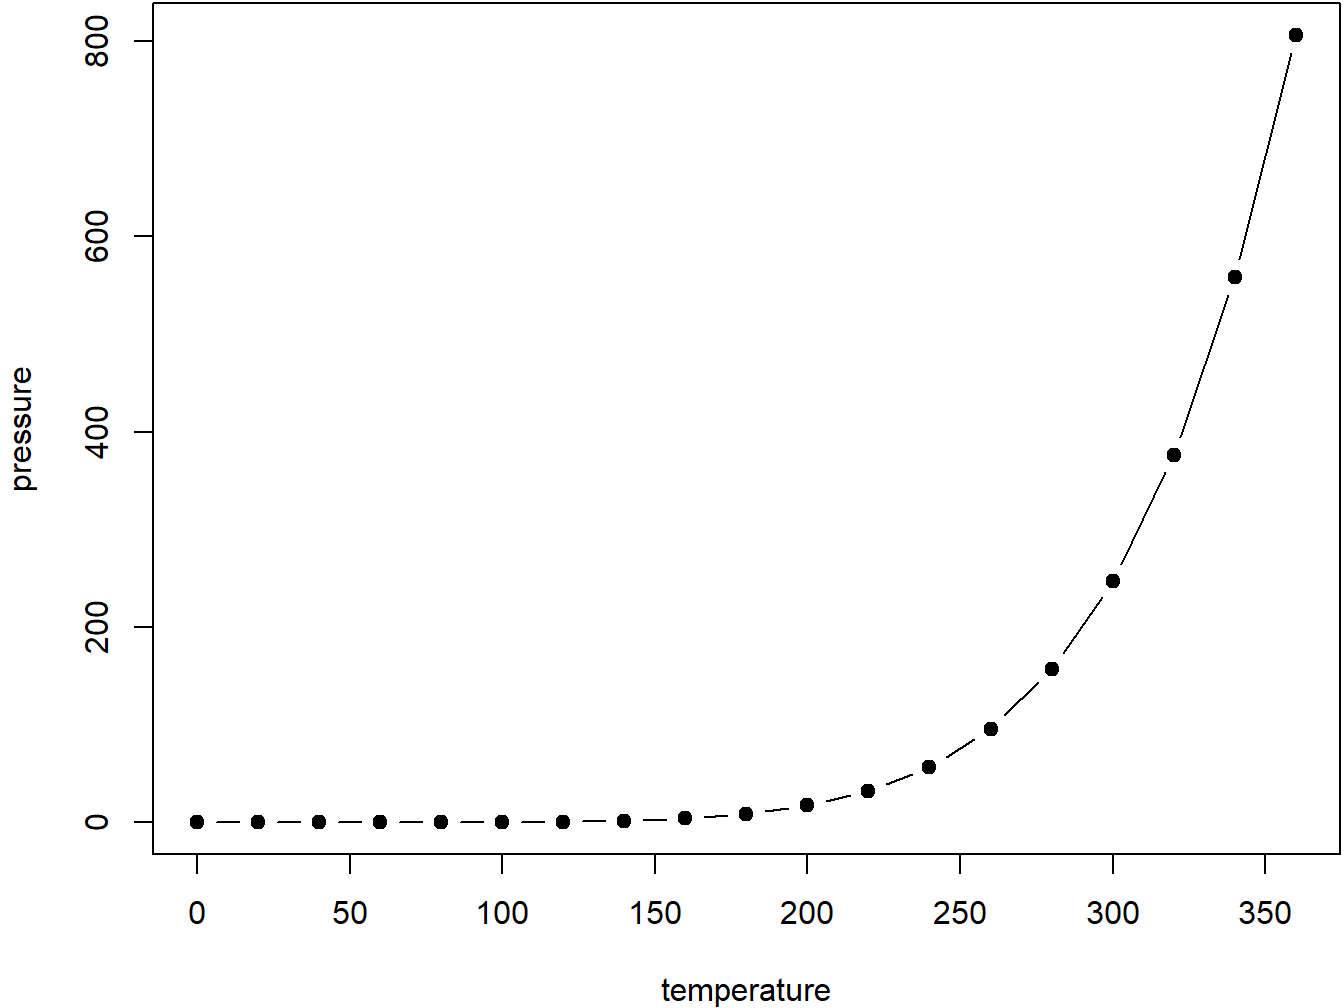
\includegraphics[width=0.8\linewidth]{irises_files/figure-latex/nice-fig-1} 

}

\caption{Here is a nice figure!}\label{fig:nice-fig}
\end{figure}

Reference a figure by its code chunk label with the \texttt{fig:} prefix, e.g., see Figure \ref{fig:nice-fig}. Similarly, you can reference tables generated from \texttt{knitr::kable()}, e.g., see Table \ref{tab:nice-tab}.

\begin{Shaded}
\begin{Highlighting}[]
\NormalTok{knitr}\SpecialCharTok{::}\FunctionTok{kable}\NormalTok{(}
  \FunctionTok{head}\NormalTok{(iris, }\DecValTok{20}\NormalTok{), }\AttributeTok{caption =} \StringTok{\textquotesingle{}Here is a nice table!\textquotesingle{}}\NormalTok{,}
  \AttributeTok{booktabs =} \ConstantTok{TRUE}
\NormalTok{)}
\end{Highlighting}
\end{Shaded}

\begin{table}

\caption{\label{tab:nice-tab}Here is a nice table!}
\centering
\begin{tabular}[t]{rrrrl}
\toprule
Sepal.Length & Sepal.Width & Petal.Length & Petal.Width & Species\\
\midrule
5.1 & 3.5 & 1.4 & 0.2 & setosa\\
4.9 & 3.0 & 1.4 & 0.2 & setosa\\
4.7 & 3.2 & 1.3 & 0.2 & setosa\\
4.6 & 3.1 & 1.5 & 0.2 & setosa\\
5.0 & 3.6 & 1.4 & 0.2 & setosa\\
\addlinespace
5.4 & 3.9 & 1.7 & 0.4 & setosa\\
4.6 & 3.4 & 1.4 & 0.3 & setosa\\
5.0 & 3.4 & 1.5 & 0.2 & setosa\\
4.4 & 2.9 & 1.4 & 0.2 & setosa\\
4.9 & 3.1 & 1.5 & 0.1 & setosa\\
\addlinespace
5.4 & 3.7 & 1.5 & 0.2 & setosa\\
4.8 & 3.4 & 1.6 & 0.2 & setosa\\
4.8 & 3.0 & 1.4 & 0.1 & setosa\\
4.3 & 3.0 & 1.1 & 0.1 & setosa\\
5.8 & 4.0 & 1.2 & 0.2 & setosa\\
\addlinespace
5.7 & 4.4 & 1.5 & 0.4 & setosa\\
5.4 & 3.9 & 1.3 & 0.4 & setosa\\
5.1 & 3.5 & 1.4 & 0.3 & setosa\\
5.7 & 3.8 & 1.7 & 0.3 & setosa\\
5.1 & 3.8 & 1.5 & 0.3 & setosa\\
\bottomrule
\end{tabular}
\end{table}

You can write citations, too. For example, we are using the \textbf{bookdown} package \citep{R-bookdown} in this sample book, which was built on top of R Markdown and \textbf{knitr} \citep{xie2015}.

\hypertarget{literature}{%
\chapter{Literature}\label{literature}}

Here is a review of existing methods.

\hypertarget{recomendaciones-internacionales-para-la-generaciuxf3n-de-estaduxedsticas-sobre-pdi-iris}{%
\section{\texorpdfstring{\textbf{Recomendaciones internacionales para la generación de estadísticas sobre PDI (IRIS)}}{Recomendaciones internacionales para la generación de estadísticas sobre PDI (IRIS)}}\label{recomendaciones-internacionales-para-la-generaciuxf3n-de-estaduxedsticas-sobre-pdi-iris}}

Borrador para revisión por parte de la Comisión de Estadística de las Naciones Unidas
(febrero de 2020)

\emph{Versión española (junio de 2021, ACNUR). La traducción oficial al español está en proceso. Consulte la versión oficial en inglés:} \url{https://ec.europa.eu/eurostat/documents/3859598/12257846/KS-GQ-20-005-EN-N.pdf/714a7ba0-7ae6-1707-fef4-984a760e0034}? t = 1610984164036

\hypertarget{section}{%
\chapter{}\label{section}}

\hypertarget{section-1}{%
\chapter{}\label{section-1}}

\hypertarget{agradecimientos}{%
\section{AGRADECIMIENTOS}\label{agradecimientos}}

Las \textbf{Recomendaciones internacionales para la generación de estadísticas sobre PDI (IRIS)} han sido desarrolladas por el subgrupo de PDI del Grupo de Expertos en Estadísticas de Personas Refugiadas y Desplazadas Internas (EGRIS), dirigido por el Servicio Conjunto de Perfiles de PDI (JIPS), con el apoyo de la División de Estadística de las Naciones Unidas (UNSD), Estadísticas de Noruega y el Centro de Monitoreo de Desplazamientos Internos (IDMC). Las recomendaciones se han elaborado en estrecha colaboración entre personas expertas de gobiernos y organizaciones regionales e internacionales, lo que garantiza una amplia gama de perspectivas.

Las personas que se listan a continuación contribuyeron a la labor en representación de países y territorios: Mowahed Hasibullah (Autoridad Nacional de Estadística e Información de Afganistán); Zabiha Asgar (Comité Estatal de Estadística de la República de Azerbaiyán); Zlatan Hadžić (Agencia de Estadística de Bosnia y Herzegovina); Oscar Iván Rico (Unidad de Víctimas del Gobierno de Colombia); Kô Fié Didier Laurent Kra (Instituto Nacional de Estadística de Costa de Marfil); Paata Shavishvili y Shorena Tsiklauri (Oficina Nacional de Estadística de Georgia); Avni Kastrati (Agencia de Estadística de Kosovo); Gohdar Mohamed y Serwan Mohamed (Oficina de Estadística de la Región del Kurdistán, Irak); Edgar Vielma Orozco (Instituto Nacional de Estadística y Geografía de México); Semiu Adeyemi Adeniran (Oficina Nacional de Estadística, Nigeria); Vebjørn Aalandslid, Helge Brunborg y Janne ThereseUtkilen (Estadística de Noruega); Lourdines Dela Cruz, Editha R. Orcilla y Henedin Palabras (Autoridad Estadística de Filipinas); Mohamed Moalim y Dahir Mohamed Noor (Ministerio de Asuntos Humanitarios y Gestión de Desastres, Somalia) y Abdirahman Mohamed Sheikh Abdi (Dirección de Estadísticas Nacionales del Ministerio de Planificación, Inversión y Desarrollo Económico, Somalia); Helen Laetitia Namirembe-Nviiri (Oficina de Estadística de Uganda); y Vadym Pishcheiko (Servicio Estatal de Estadística de Ucrania).

La labor contó también con la participación de las siguientes personas, quienes actuaron en representación de organizaciones internacionales y regionales: Léandre Foster Ngogang Wandji (Centro Africano de Estadística, Comisión Económica de las Naciones Unidas para África, UNECA); Maurice Mubila (Banco Africano de Desarrollo, AfDB); Adrián Calvo-Valderrama y Avigail Shai (IDMC); Duncan Sullivan y Eduardo Zambrano (Organización Internacional para las Migraciones, OIM); Tilman Brück (Centro Internacional de Seguridad y Desarrollo, ISDC); Natalia Krynsky Baal, Marte Claussen, Corina Demottaz, Lauren Herby (Consultora), Laura Kivela, Devora Levakova y Mihaela Darii Sposato (JIPS); Martina Caterina (Representante de la Relatoría Especial sobre los derechos humanos de los desplazados internos); Kashif Rehman, Javier Terán y Greta Zeender (Oficina de Coordinación de Asuntos Humanitarios de las Naciones Unidas, OCHA); Atle Solberg (Plataforma sobre el Desplazamiento por Desastres, PDD); Christian Baureder, Daniel MacGuire, Petra Nahmias, Kimberly Roberson, Aina Helen Sætre y Mary Strode (Consultora) (Agencia de las Naciones Unidas para los Refugiados, ACNUR); Vibeke Oestreich Nielsen (UNSD); y Xavier Devictor, Caroline Sergeant, Emi Suzuki y Paolo Verme (Grupo del Banco Mundial).

Las organizaciones antes mencionadas han hecho contribuciones sustanciales a través de su personal. Agradecemos especialmente a Natalia Krynsky Baal, Devora Levakova, Vibeke Oestreich Nielsen y Mary Strode por su contribución a la redacción de las recomendaciones, y a Corina Demottaz por el diseño visual. La Asociación Europea de Libre Comercio (AELC), Eurostat, JIPS, Estadísticas de Noruega, el ACNUR y el Banco Mundial hicieron contribuciones financieras.

\begin{enumerate}
\def\labelenumi{\arabic{enumi}.}
\item ~
  \hypertarget{tabla-de-contenido}{%
  \section{Tabla de contenido}\label{tabla-de-contenido}}
\end{enumerate}

\hypertarget{section-2}{%
\chapter{}\label{section-2}}

Y

\protect\hyperlink{_Toc71834729}{AGRADECIMIENTOS 2}

\protect\hyperlink{_Toc71834730}{A.Tabla de contenido 3}

\protect\hyperlink{_Toc71834731}{B.Listado de recuadros, figuras y tablas 5}

\protect\hyperlink{_Toc71834732}{C.Abreviaturas 6}

\textbf{\protect\hyperlink{_Toc71834733}{CAPÍTULO 1}INTRODUCCIÓN 7}

\protect\hyperlink{_Toc71834734}{A.Sobre la necesidad de contar con recomendaciones para la generación de estadísticas sobre personas desplazadas internas 7}

\protect\hyperlink{_Toc71834735}{B.Proceso de elaboración de las recomendaciones 9}

\protect\hyperlink{_Toc71834736}{C.Justificación y alcance 11}

\protect\hyperlink{_Toc71834737}{D.Vínculos con otros productos del grupo de expertos en estadísticas sobre personas refugiadas y desplazadas internas 12}

\protect\hyperlink{_Toc71834738}{E.Disposición de las recomendaciones 13}

\textbf{\protect\hyperlink{_Toc71834739}{CAPÍTULO 2. POLÍTICAS PÚBLICAS Y MARCO JURÍDICO 15}}

\protect\hyperlink{_Toc71834740}{A.Introducción 15}

\protect\hyperlink{_Toc71834741}{B.Marcos normativos para la protección de PDI 15}

\_\protect\hyperlink{_Toc71834742}{1.}\_\_Marco internacional 15\_

\_\protect\hyperlink{_Toc71834743}{2.}\_\_Instrumentos regionales 16\_

\_\protect\hyperlink{_Toc71834744}{3.}\_\_Leyes y políticas nacionales 17\_

\_\protect\hyperlink{_Toc71834745}{4.}\_\_Definición de PDI en los Principios Rectores 18\_

\protect\hyperlink{_Toc71834746}{C.Elementos de la definición de PDI en los Principios Rectores 19}

\_\protect\hyperlink{_Toc71834747}{1.}\_\_Persona forzada u obligada a huir o a marcharse 19\_

\_\protect\hyperlink{_Toc71834748}{2.}\_\_Hogares o lugares de residencia habitual 19\_

\_\protect\hyperlink{_Toc71834749}{3.}\_\_El desplazamiento como resultado o el desplazamiento como medio para evitar algo 20\_

\_\protect\hyperlink{_Toc71834750}{4.}\_\_Causas 21\_

\_\protect\hyperlink{_Toc71834751}{5.}\_\_Cruce de fronteras reconocidas internacionalmente 23\_

\_\protect\hyperlink{_Toc71834752}{6.}\_\_Otros asuntos no mencionadas explícitamente en los Principios Rectores 25\_

\protect\hyperlink{_Toc71834753}{D.Soluciones duraderas y fin de los desplazamientos internos 26}

\protect\hyperlink{_Toc71834754}{E.Conclusión 28}

\textbf{\protect\hyperlink{_Toc71834755}{CAPÍTULO 3.}DESARROLLO DE UN MARCO ESTADÍSTICO 29}

\protect\hyperlink{_Toc71834756}{A.Introducción 29}

\protect\hyperlink{_Toc71834757}{B.Marco estadístico del desplazamiento interno 29}

\_\protect\hyperlink{_Toc71834758}{1.}\_\_Categorías incluidas en el marco estadístico del desplazamiento interno 29\_

\_\protect\hyperlink{_Toc71834759}{2.}\_\_Categorías de personas desplazadas no incluidas en el marco estadístico del desplazamiento interno 34\_

\protect\hyperlink{_Toc71834760}{C.Definición de la población estadística y de flujos de PDI 37}

\_\protect\hyperlink{_Toc71834761}{1.}\_\_Población estadística 38\_

\_\protect\hyperlink{_Toc71834762}{2.}\_\_Flujos 39\_

\protect\hyperlink{_Toc71834763}{D.Cómo determinar el aumento: cuatro condiciones 41}

\_\protect\hyperlink{_Toc71834764}{1.}\_\_Han sido forzadas u obligadas a desplazarse de su lugar de residencia habitual por un acontecimiento causante 42\_

\_\protect\hyperlink{_Toc71834765}{2.}\_\_Residían en el lugar y en el momento en que se produjo el acontecimiento 43\_

\_\protect\hyperlink{_Toc71834766}{3.}\_\_Han estado viviendo físicamente fuera de la vivienda en la que vivían en el momento del acontecimiento causante 44\_

\_\protect\hyperlink{_Toc71834767}{4.}\_\_Se encuentran dentro de las fronteras internacionalmente reconocidas del país 45\_

\protect\hyperlink{_Toc71834768}{E.Resumen de recomendaciones 46}

\textbf{\protect\hyperlink{_Toc71834769}{CAPÍTULO 4. SOLUCIONES DURADERAS Y PRINCIPALES VULNERABILIDADES RELACIONADAS CON EL DESPLAZAMIENTO 47}}

\protect\hyperlink{_Toc71834770}{A.Introducción 47}

\protect\hyperlink{_Toc71834771}{B.Definición de criterios para las dos medidas 47}

\_\protect\hyperlink{_Toc71834772}{1.}\_\_Recursos relevantes 47\_

\_\protect\hyperlink{_Toc71834773}{2.}\_\_Criterios de vulnerabilidad relacionados con el desplazamiento 51\_

\protect\hyperlink{_Toc71834774}{C.Medida del progreso hacia soluciones duraderas 56}

\_\protect\hyperlink{_Toc71834775}{1.}\_\_Esquema de la medida del progreso 56\_

\_\protect\hyperlink{_Toc71834776}{1.}\_\_Usos de la medida del progreso 60\_

\protect\hyperlink{_Toc71834777}{D.Medida compuesta para superar las principales vulnerabilidades relacionadas con el desplazamiento 61}

\_\protect\hyperlink{_Toc71834778}{1.}\_\_Alcance de la medida compuesta 62\_

\_\protect\hyperlink{_Toc71834779}{2.}\_\_Esquema de la medida compuesta 63\_

\protect\hyperlink{_Toc71834780}{E.Resumen de recomendaciones 66}

\textbf{\protect\hyperlink{_Toc71834781}{CAPÍTULO 5. VARIABLES Y TABULACIONES 67}}

\protect\hyperlink{_Toc71834782}{A.Introducción 67}

\protect\hyperlink{_Toc71834783}{B.Variables clasificatorias básicas 67}

\protect\hyperlink{_Toc71834784}{C.Flujos de PDI y poblaciones relacionadas con ellas 68}

\_\protect\hyperlink{_Toc71834785}{1.}\_\_Estadísticas básicas sobre el aumento 68\_

\_\protect\hyperlink{_Toc71834786}{2.}\_\_Estadísticas básicas sobre disminución de PDI 69\_

\_\protect\hyperlink{_Toc71834787}{3.}\_\_Estadísticas básicas de los flujos entre las subcategorías de PDI 70\_

\protect\hyperlink{_Toc71834788}{D.Población estadística de PDI y poblaciones relacionadas con ellas 70}

\_\protect\hyperlink{_Toc71834789}{1.}\_\_Estadísticas básicas sobre la población estadística 70\_

\_\protect\hyperlink{_Toc71834790}{2.}\_\_Estadísticas básicas de progreso 71\_

\protect\hyperlink{_Toc71834791}{E.Indicadores clave de la población estadística de PDI y poblaciones relacionadas con ellas 72}

\protect\hyperlink{_Toc71834792}{F.Resumen de recomendaciones 72}

\textbf{\protect\hyperlink{_Toc71834793}{CAPÍTULO 6. FUENTES DE DATOS PARA LA RECOPILACIÓN DE ESTADÍSTICAS SOBRE LAS PDI 73}}

\protect\hyperlink{_Toc71834794}{A.Introducción 73}

\protect\hyperlink{_Toc71834795}{B.Panorama de las fuentes de datos sobre PDI 73}

\_\protect\hyperlink{_Toc71834796}{1.}\_\_El censo de población y vivienda 76\_

\_\protect\hyperlink{_Toc71834797}{2.}\_\_Encuestas de hogares por muestreo 81\_

\_\protect\hyperlink{_Toc71834798}{3.}\_\_Datos y registros administrativos 86\_

\_\protect\hyperlink{_Toc71834799}{4.}\_\_Fuentes de datos alternativas 89\_

\protect\hyperlink{_Toc71834800}{C.Datos operativos recogidos con fines humanitarios 91}

\_\protect\hyperlink{_Toc71834801}{1.}\_\_Diferencias entre los datos operativos y las estadísticas oficiales 91\_

\_\protect\hyperlink{_Toc71834802}{2.}\_\_Descripción de las fuentes de datos operativos cuantitativos 92\_

\_\protect\hyperlink{_Toc71834803}{3.}\_\_Descripción de las fuentes cualitativas de datos operativos 93\_

\_\protect\hyperlink{_Toc71834804}{4.}\_\_Consideraciones sobre la calidad de los datos operativos 94\_

\protect\hyperlink{_Toc71834805}{D.Integración de datos 94}

\_\protect\hyperlink{_Toc71834806}{1.}\_\_Consideraciones sobre las estadísticas de PDI 94\_

\_\protect\hyperlink{_Toc71834807}{2.}\_\_Enfoques para el cotejo de datos 95\_

\protect\hyperlink{_Toc71834808}{E.Seleccionar entre diferentes fuentes de datos 96}

\_\protect\hyperlink{_Toc71834809}{1.}\_\_Cómo evaluar las ventajas e inconvenientes de las fuentes de datos 96\_

\_\protect\hyperlink{_Toc71834810}{2.}\_\_Cómo superar las vulnerabilidades relacionadas con los desplazamientos 97\_

\protect\hyperlink{_Toc71834811}{F.Resumen de recomendaciones 100}

\textbf{\protect\hyperlink{_Toc71834812}{CAPÍTULO 7}COORDINACIÓN DE LAS ESTADÍSTICAS SOBRE PDI 102}

\protect\hyperlink{_Toc71834813}{A.Introducción 102}

\protect\hyperlink{_Toc71834814}{B.Coordinación nacional de estadísticas sobre PDI 103}

\_\protect\hyperlink{_Toc71834815}{1.}\_\_Sistema estadístico nacional 104\_

\_\protect\hyperlink{_Toc71834816}{2.}\_\_Cumplimiento de las normas de calidad estadística 105\_

\_\protect\hyperlink{_Toc71834817}{1.}\_\_Datos operativos para responder a las crisis de desplazamiento 111\_

\protect\hyperlink{_Toc71834818}{C.Coordinación internacional de estadísticas sobre PDI 117}

\_\protect\hyperlink{_Toc71834819}{1.}\_\_Organizaciones y procesos internacionales pertinentes 117\_

\_\protect\hyperlink{_Toc71834820}{2.}\_\_Principios relevantes para la elaboración de estadísticas internacionales 120\_

\_\protect\hyperlink{_Toc71834821}{3.}\_\_Recopilación de estadísticas para comparaciones internacionales 121\_

\protect\hyperlink{_Toc71834822}{D.Resumen de recomendaciones 122}

\_\protect\hyperlink{_Toc71834823}{1.}\_\_Mejorar la coordinación estadística nacional 123\_

\_\protect\hyperlink{_Toc71834824}{2.}\_\_Mejorar la coordinación estadística internacional y regional 125\_

\begin{enumerate}
\def\labelenumi{\arabic{enumi}.}
\item ~
  \hypertarget{listado-de-recuadros-figuras-y-tablas}{%
  \section{Listado de recuadros, figuras y tablas}\label{listado-de-recuadros-figuras-y-tablas}}
\end{enumerate}

\protect\hyperlink{_Toc70629913}{Recuadro 3.1 Definición de PDI (o personas que tienen necesidades de protección y vulnerabilidades relacionadas con el desplazamiento) 32}

\protect\hyperlink{_Toc70629914}{Recuadro 3.2 Definición estadística de la migración 36}

\href{/C:\%5CUsers\%5CMariana\%5CDocuments\%5C04-TRABAJO\%5CACNUR\%5CTraducciones\%5C04_Abril_2021\%5CACNUR\%2020210422-1\%5CIRIS\%202020.3486_src_EN_revised_140820_ESP_REV_mfa.docx\#_Toc70629915}{Recuadro 3.3 Residencia usual y residencia habitual 44}

\href{/C:\%5CUsers\%5CMariana\%5CDocuments\%5C04-TRABAJO\%5CACNUR\%5CTraducciones\%5C04_Abril_2021\%5CACNUR\%2020210422-1\%5CIRIS\%202020.3486_src_EN_revised_140820_ESP_REV_mfa.docx\#_Toc70629916}{Recuadro 3.4 Definición estadística del país de residencia usual 46}

\protect\hyperlink{_Toc70629917}{Figura 3.1 Categorías de población en el marco estadístico de desplazamiento interno 30}

\protect\hyperlink{_Toc70629918}{Figura 3.2 Personas desplazadas por la fuerza que cruzan una frontera internacionalmente reconocida y su relación con la población estadística de PDI 34}

\protect\hyperlink{_Toc70629919}{Figura 3.3 Aumento y disminución de flujos de la población estadística de PDI 39}

\protect\hyperlink{_Toc70629920}{Figura 4.1 Criterios del IASC para soluciones duraderas: proceso propuesto para identificar indicadores básicos específicos para cada contexto 49}

\protect\hyperlink{_Toc70629921}{Figura 4.2Ilustración de los pros y los contras de la identificación de grupos de población comparativos 55}

\href{/C:\%5CUsers\%5CMariana\%5CDocuments\%5C04-TRABAJO\%5CACNUR\%5CTraducciones\%5C04_Abril_2021\%5CACNUR\%2020210422-1\%5CIRIS\%202020.3486_src_EN_revised_140820_ESP_REV_mfa.docx\#_Toc70629922}{Figura 4.3 Demostración de los resultados analíticos de la medida del progreso hacia soluciones duraderas 58}

\protect\hyperlink{_Toc70629923}{Figura 4.4 Metodología para la medida compuesta 65}

\protect\hyperlink{_Toc70629924}{Tabla 4.1 Se recomienda desglosar los indicadores de los ODS por categoría de desplazamiento forzado según el ámbito político prioritario 50}

\protect\hyperlink{_Toc70629925}{Tabla 4.2 Criterios de soluciones duraderas del IASC y subcriterios identificados 52}

\protect\hyperlink{_Toc70629926}{Tabla 4.3 Criterios y subcriterios incluidos en la medida compuesta 63}

\protect\hyperlink{_Toc70629927}{Tabla 6.1 Consideraciones clave sobre la calidad de las estadísticas de PDI 75}

\protect\hyperlink{_Toc70629928}{Tabla 6.2 Diferencias entre los datos operativos y las estadísticas oficiales () 92}

\protect\hyperlink{_Toc70629929}{Tabla 6.3 Resumen de las principales fuentes de datos relacionados con el desplazamiento 96}

\protect\hyperlink{_Toc70629930}{Tabla 6.4Fuentes de datos y uso en el análisis de las vulnerabilidades relacionadas con el desplazamiento 100}

\begin{enumerate}
\def\labelenumi{\arabic{enumi}.}
\item ~
  \hypertarget{abreviaturas}{%
  \section{Abreviaturas}\label{abreviaturas}}
\end{enumerate}

\begin{longtable}[]{@{}
  >{\raggedright\arraybackslash}p{(\columnwidth - 2\tabcolsep) * \real{0.50}}
  >{\raggedright\arraybackslash}p{(\columnwidth - 2\tabcolsep) * \real{0.50}}@{}}
\toprule
CCSA & Comité para la Coordinación de Actividades Estadísticas \\
\midrule
\endhead
DRC & Consejo Danés para los Refugiados \\
DTM & Matriz de seguimiento del desplazamiento \\
EGRIS & Grupo de expertos en estadísticas sobre personas refugiadas y desplazadas internas \\
IASC & Comité Permanente entre Organismos \\
IDMC & Centro de Monitoreo del Desplazamiento Interno \\
PDI & Persona desplazada interna \\
DIH & Derecho internacional humanitario \\
DIDH & Derecho internacional de los derechos humanos \\
OIM & Organización Internacional para las Migraciones \\
IRIS & \emph{Recomendaciones internacionales para la generación de estadísticas sobre PDI} \\
IRRS & \emph{Recomendaciones internacionales para la generación de estadísticas sobre personas refugiadas} \\
JIPS & Servicio conjunto de perfiles de PDI \\
ONG & Organización no gubernamental \\
NRC & Consejo Noruego para las Personas Refugiadas \\
NSDS & Estrategias nacionales para el desarrollo de estadísticas \\
ONE & Oficina nacional de estadística \\
SEN & Sistema estadístico nacional \\
OCHA & Oficina de las Naciones Unidas para la Coordinación de Asuntos Humanitarios \\
OCDE & Organización para la Cooperación y el Desarrollo Económico \\
PDD & Plataforma sobre desplazamientos por desastres \\
NIP & Número de identificación personal \\
ODS & Objetivo de Desarrollo Sostenible \\
ONU & Organización de las Naciones Unidas \\
UNFPOS & \emph{Principios fundamentales de las estadísticas oficiales de las Naciones Unidas} \\
ACNUR & Agencia de las Naciones Unidas para los Refugiados \\
UNSC & Comisión de Estadística de las Naciones Unidas \\
UNSD & División de Estadística de las Naciones Unidas \\
UN-SQAF & \emph{Marco de garantía de calidad de las estadísticas de las Naciones Unidas} \\
PMA & Programa Mundial de Alimentos \\
\bottomrule
\end{longtable}

\hypertarget{capuxedtulo-1-introducciuxf3n}{%
\chapter{CAPÍTULO 1 INTRODUCCIÓN}\label{capuxedtulo-1-introducciuxf3n}}

\begin{enumerate}
\def\labelenumi{\arabic{enumi}.}
\item ~
  \hypertarget{sobre-la-necesidad-de-contar-con-recomendaciones-para-la-generaciuxf3n-de-estaduxedsticas-sobre-personas-desplazadas-internas}{%
  \section{Sobre la necesidad de contar con recomendaciones para la generación de estadísticas sobre personas desplazadas internas}\label{sobre-la-necesidad-de-contar-con-recomendaciones-para-la-generaciuxf3n-de-estaduxedsticas-sobre-personas-desplazadas-internas}}
\item
  El objetivo de este capítulo introductorio es contextualizar las recomendaciones, así como presentar la justificación y el alcance del propio informe. Por tanto, en este capítulo se presentan brevemente los antecedentes, se identifican los vínculos clave entre estas recomendaciones y otros esfuerzos, incluidas las \emph{Recomendaciones internacionales para la generación de estadísticas sobre personas refugiadas} (IRRS, por sus siglas en inglés) (
  \# 1
  ), y se resumen la estructura de las recomendaciones y el proceso a través del cual se desarrollaron.
\item
  El término `personas desplazadas internas' (en adelante, ``PDI'') se refiere a ``las personas o grupos de personas que se han visto forzadas u obligadas a escapar o huir de su hogar o de su lugar de residencia habitual ---en particular, como resultado o para evitar los efectos de un conflicto armado, de situaciones de violencia generalizada, de violaciones de los derechos humanos o de catástrofes naturales o provocadas por el ser humano---, y que no han cruzado una frontera estatal internacionalmente reconocida'' (
  \# 2
  ). Esta definición sirve de base para la recopilación de estadísticas oficiales y para las recomendaciones contenidas en este informe.
\item
  En la actualidad, las PDI representan la mayor parte de las poblaciones desplazadas en el mundo. Los datos y las estadísticas sobre las PDI se requieren para fundamentar las políticas públicas que se generan en respuesta al desplazamiento interno. Los datos sobre las PDI son especialmente útiles porque proporcionan un punto de referencia a partir del cual se puede monitorear la situación de las poblaciones de PDI, así como medir los logros de las políticas y los programas relacionados. Sin embargo, al día de hoy siguen siendo escasas las guías internacionales sobre la mejor manera de generar estadísticas oficiales de buena calidad sobre las PDI; además, en lugar de basarse en estadísticas oficiales, muchos de los datos disponibles parten de los datos operativos que recaban las agencias humanitarias como parte de sus programas de asistencia. En vista de que los datos sobre las PDI se recaban con respecto a las personas afectadas por conflictos, catástrofes o violencia, en la fase inicial del desplazamiento puede ser difícil o imposible recopilar estadísticas oficiales, y los datos operativos suelen ser la mejor opción disponible. Estas recomendaciones analizan las funciones de ambos tipos de datos.
\item
  Las normas internacionales de calidad (
  \# 3
  ) exigen que las estadísticas oficiales sean consistentes entre sí y en el transcurso del tiempo; además, deben ser comparables entre regiones y países. De igual manera, es importante que las estadísticas oficiales permitan que las organizaciones del sistema estadístico de un país utilicen conjuntamente datos relacionados que proceden de distintas fuentes. Como parte de su evaluación de las estadísticas sobre PDI, el Grupo de expertos en estadísticas sobre personas refugiadas y desplazadas internas (EGRIS, por sus gilas en inglés) presentó un informe sobre asuntos de calidad estadística. Las estadísticas sobre PDI se presentaron en el \emph{Informe técnico sobre estadísticas de personas desplazadas internas} (
  \# 4
  ), en el 49º período de sesiones de la Comisión de Estadística de las Naciones Unidas (UNSC) en 2018, donde se adoptaron formalmente.
\item
  Las estadísticas de buena calidad sobre el desplazamiento constituyen un requisito para el seguimiento y la aplicación de una serie de programas y acuerdos internacionales. Entre ellos se encuentran:
\item
  La Agenda 2030 para el Desarrollo Sostenible y el compromiso de no dejar a nadie atrás, incluidas las PDI (
  \# 5
  );
\item
  Marco de Sendai para la Reducción del Riesgo de Desastres 2015-2030 (
  \# 6
  );
\item
  Acuerdo de París de la Convención Marco de las Naciones Unidas sobre el Cambio Climático (
  \# 7
  );
\item
  Programa de protección de la Iniciativa Nansen para las personas desplazadas a través de las fronteras por catástrofes (
  \# 8
  );
\item
  Agenda para la Humanidad (
  \# 9
  );
\item
  Agenda 2063 para África (
  \# 10
  );
\item
  Plan de acción de la Cumbre de La Valeta (
  \# 11
  ); y
\item
  Nueva Agenda Urbana (
  \# 12
  ).
\item
  Aunado a lo anterior, se necesitan estadísticas confiables e integrales sobre los desplazamientos internos para monitorear los avances hacia el ambicioso llamado del Secretario General de la ONU en cuanto a la reducción de desplazamientos internos ---nuevos y prolongados--- en al menos 50\% para el año 2030 (
  \# 13
  ). De igual manera, las estadísticas serán necesarias para fundamentar acciones en el marco del \emph{Pacto Mundial para una Migración Segura, Ordenada y Regular} (
  \# 14
  ) y el \emph{Pacto Mundial sobre los Refugiados} (
  \# 15
  ), aunque ninguno aborda explícitamente el desplazamiento interno, así como otros procesos políticos en la materia (
  \# 16
  ). Si bien varias iniciativas internacionales que cuentan con el apoyo de socios de desarrollo se relacionan con la elaboración de estadísticas sobre PDI, la responsabilidad última siempre recaerá en los gobiernos nacionales.
\item
  Son variadas las prácticas nacionales e internacionales para traducir la definición internacional de PDI en un concepto estadístico medible. Esta diversidad refleja diferencias de interpretación y respuestas \emph{ad hoc} a los retos prácticos, técnicos y de política pública que surgen en contextos de desplazamiento. Aunque las estadísticas en muchos contextos se apartan de la definición global de PDI que versa en los \emph{Principios Rectores de los Desplazamientos Internos}, existen puntos importantes en común. La UNSC ha reconocido la necesidad de mejorar la práctica utilizando un marco estadístico acordado internacionalmente para esta población; además, ha solicitado recomendaciones que esclarezcan los retos conceptuales y permitan una mejor comparabilidad de los datos.
\item ~
  \hypertarget{proceso-de-elaboraciuxf3n-de-las-recomendaciones}{%
  \section{Proceso de elaboración de las recomendaciones}\label{proceso-de-elaboraciuxf3n-de-las-recomendaciones}}
\item
  A raíz de los debates que tuvieron lugar en 2015 en relación con un documento sobre estadísticas de personas refugiadas (
  \# 17
  ), el 46º periodo de sesiones de la UNSC solicitó que se organizara una conferencia de expertos para profundizar en el asunto. Sobre la base de los resultados de esta conferencia de expertos, se presentó un informe técnico a la UNSC en el que se recomendaba la elaboración de un manual de estadísticas oficiales sobre personas refugiadas (
  \# 18
  ). Además, algunas conversaciones sobre el tema durante el 47º período de sesiones de 2016 dieron lugar a otra decisión relativa a la creación de un Grupo internacional de expertos en estadísticas sobre personas refugiadas y desplazadas internas (EGRIS, por su siglas en inglés), cuya integración incluiría representantes de autoridades nacionales y de organizaciones estadísticas regionales e internacionales, así como otros expertos técnicos.
\item
  Estadísticas de Noruega, el Instituto Turco de Estadística, Eurostat, la Agencia de las Naciones Unidas para los Refugiados (ACNUR), el Servicio conjunto de perfiles de personas desplazadas internas (JIPS), el Banco Mundial y la División de Estadística de las Naciones Unidas (UNSD) copresiden el EGRIS. En particular, la UNSC solicitó que el alcance del trabajo del EGRIS incluyera tanto a las PDI como a las personas refugiadas. Aunado a ello, se creó un subgrupo del EGRIS para trabajar en la elaboración del informe técnico sobre las estadísticas de las PDI.
\item
  La UNSC comisionó al EGRIS la elaboración de dos documentos para el 49º período de sesiones de la UNSC en 2018, tras una consulta mundial (
  \# 19
  ). Estos dos documentos, las IRRS y el \emph{Informe Técnico sobre Estadísticas de Personas Desplazadas Internas}, fueron acogidos con satisfacción (
  \# 20
  ) y aprobados por la Comisión:
\item
  En el 49º período de sesiones de la UNSC en 2018 se determinó lo siguiente con respecto a estos dos documentos y con relación a los pasos propuestos en el \emph{Informe del Grupo de Expertos en Estadísticas sobre Refugiados y Desplazados Internos} (Decisiones señaladas a la atención del Consejo: 49/115 (
  \# 21
  )):
\item
  ``Apoyó la propuesta de actualizar el informe técnico relativo a las estadísticas sobre los desplazados internos mediante una serie de recomendaciones'' (es decir, las \emph{Recomendaciones internacionales para la generación de estadísticas sobre PDI, IRIS).}
\item
  ``Reconoció las dificultades en la aplicación de las recomendaciones sobre las estadísticas relativas a los refugiados y los desplazados internos, y expresó su apoyo a la elaboración de un manual de compiladores para proporcionar orientación práctica y una metodología perfeccionada en la recopilación de estadísticas sobre los refugiados y los desplazados internos''. (Esto se convertirá en el \emph{Manual para compiladores de estadísticas sobre las personas refugiadas y desplazadas internas.)}
\item
  Solicitó que las recomendaciones en materia de estadísticas sobre los desplazados internos y el manual del compilador se presentaran a la Comisión en su 51º período de sesiones, en 2020.
\item
  Además, la membresía de la UNSC:
\item
  "Reconoció la importancia de un marco de estadísticas armonizadas sobre los refugiados y los desplazados internos para la comparabilidad de los datos en el interior de un país y entre países y organismos internacionales, e hizo hincapié en que se utilizaran todas las fuentes de datos, incluidos los censos de población, las encuestas por muestreo y las fuentes administrativas;
\item
  Expresó la necesidad de establecer definiciones claras de los refugiados, los migrantes y los desplazados internos, y la necesidad de desarrollar la capacidad estadística en el plano nacional para apoyar a los Estados Miembros en el mejoramiento de la calidad y disponibilidad de estadísticas sobre los refugiados y los desplazados internos, e invitó a las organizaciones internacionales y regionales a apoyar a los Estados Miembros en este sentido, cuando estos lo solicitaran; y
\item
  Puso de relieve la necesidad de mejorar la coordinación de las diferentes necesidades de datos entre las Naciones Unidas, Eurostat y otras organizaciones internacionales pertinentes" (
  \# 22
  ).
\item
  La redacción de las IRIS es el resultado de esta decisión. Las recomendaciones fueron elaboradas por el subgrupo del EGRIS sobre estadísticas de PDI, dirigido por JIPS con el apoyo de Estadísticas de Noruega, la División de Estadística de las Naciones Unidas y el Centro de Seguimiento de los Desplazamientos Internos (IDMC). La integración del subgrupo comprendía representantes de organismos gubernamentales, incluidas las oficinas nacionales de estadística (ONE) y organismos responsables de las estadísticas sobre personas desplazadas internas (
  \# 23
  ). Estas personas participaron formalmente en dos sesiones presenciales después de que todos los países recibieron las invitaciones correspondientes durante y después del 47º período de sesiones de la UNSC en 2016. En conjunto, representan una variedad de regiones y tipos de situaciones de desplazamiento.
\item
  El subgrupo se benefició también de las aportaciones de expertos técnicos del ACNUR, de la Representación de la Relatoría Especial sobre los Derechos Humanos de los Desplazados Internos, de la Organización Internacional para las Migraciones (OIM), de la Oficina de Coordinación de Asuntos Humanitarios de las Naciones Unidas (OCHA), del Centro Africano de Estadística de la Comisión Económica de las Naciones Unidas para África (UNECA), del Banco Africano de Desarrollo, del Banco Mundial, del Centro Internacional de Seguridad y Desarrollo (ISDC) y de la Plataforma sobre Desplazamiento por Desastres (PDD).
\item
  Las IRIS son el resultado de un amplio y profundo proceso colaborativo que se ha basado en la experiencia y los conocimientos de quienes integran el subgrupo de PDI. Tras las consultas sobre el primer borrador ---el cual se elaboró a partir del \emph{Informe técnico sobre estadísticas de desplazados internos}, que fue revisado y debatido en Kampala en diciembre de 2018 y en Ankara en febrero de 2019--- se crearon dos subgrupos de trabajo para abordar temas más complejos. Entre ellos se incluyen recomendaciones en torno a la coordinación global de las estadísticas sobre PDI y recomendaciones para medir la disminución de la población estadística para completar el marco estadístico de los desplazamientos internos (
  \# 24
  ). Los resultados de estos subgrupos de trabajo se incorporaron al borrador, y fueron revisados y finalizados por el subgrupo de PDI y el grupo directivo del EGRIS. Por último, antes de su presentación a la UNSC en 2020, las recomendaciones se sometieron a una consulta mundial, facilitada por la División de Estadística de las Naciones Unidas.
\item ~
  \hypertarget{justificaciuxf3n-y-alcance}{%
  \section{Justificación y alcance}\label{justificaciuxf3n-y-alcance}}
\item
  El objetivo de este informe es ofrecer recomendaciones sobre la elaboración y difusión de estadísticas sobre desplazamientos internos. Esto contribuirá a reforzar las políticas públicas basadas en datos, así como las respuestas nacionales a largo plazo frente al desplazamiento:
\item
  aumentando la visibilidad del desplazamiento interno por medio de pruebas más sólidas;
\item
  mejorando la calidad, comparabilidad, accesibilidad y coherencia de las estadísticas sobre las PDI;
\item
  informando mejor sobre los esfuerzos de las autoridades nacionales para garantizar la protección y la asistencia que reciben las PDI, así como permitiendo que se concreten soluciones duraderas;
\item
  apoyando los análisis del impacto de los desplazamientos internos y los avances hacia soluciones duraderas para las poblaciones afectadas;
\item
  sistematizando los análisis de los datos de vulnerabilidad relativos a los desplazamientos y seleccionando mejor a las poblaciones que necesitan intervenciones humanitarias y de desarrollo como respuesta;
\item
  apoyando la inclusión del desplazamiento interno en los planes de desarrollo locales y nacionales, así como la presentación de informes sobre los Objetivos de Desarrollo Sostenible (ODS).
\item
  El enfoque principal de este informe es la preparación de estadísticas oficiales sobre las PDI; sin embargo, algunos elementos son también aplicables a los datos operativos sobre las PDI que se generan en el desarrollo de una respuesta humanitaria. Los datos operativos no suelen cumplir con los requisitos de las estadísticas oficiales; no obstante, debido a la falta de estadísticas oficiales sobre las PDI, los datos operativos podrían informar la producción de nuevas estadísticas oficiales o podrían facilitar la transición a las mismas. Estas recomendaciones también deberían contribuir a mejorar la calidad y la coherencia de los datos operativos, tanto para mejorar su accesibilidad en favor del público usuario como para facilitar su sustitución con estadísticas oficiales elaboradas por autoridades nacionales, o bien, para facilitar su transición a las estadísticas oficiales.
\item
  Por lo general, se consideran estadísticas oficiales aquellas elaboradas y publicadas por dependencias gubernamentales u otros organismos públicos, como las organizaciones internacionales. La Organización para la Cooperación y el Desarrollo Económico (OCDE) define las estadísticas oficiales como ``las estadísticas difundidas por el sistema estadístico nacional, salvo las que se declaran explícitamente no oficiales''. Eurostat tiene una definición similar, pero añade la base legal para la recopilación de datos y las normas profesionales (
  \# 25
  ). La ONU no cuenta con una definición formal, pero ofrece diez \emph{Principios fundamentales de las estadísticas oficiales}, adoptados por la Asamblea General de la ONU en 2014 (UNFPOS; ver capítulo 7 para conocer más detalles).
\item
  Con base en el \emph{Informe técnico sobre estadísticas de desplazados internos} presentado en el 49º período de sesiones de la UNSC en 2018, el presente documento ofrece recomendaciones sobre cómo mejorar la calidad y la disponibilidad de las estadísticas sobre PDI para su consideración en el 51º período de sesiones de la UNSC en 2020.
\item ~
  \hypertarget{vuxednculos-con-otros-productos-del-grupo-de-expertos-en-estaduxedsticas-sobre-personas-refugiadas-y-desplazadas-internas}{%
  \section{Vínculos con otros productos del grupo de expertos en estadísticas sobre personas refugiadas y desplazadas internas}\label{vuxednculos-con-otros-productos-del-grupo-de-expertos-en-estaduxedsticas-sobre-personas-refugiadas-y-desplazadas-internas}}
\item
  Aunque se trata de un producto independiente, el presente informe se apega a las IRRS, las cuales, en la medida de lo posible, fueron también desarrolladas por el EGRIS. El vínculo entre estos dos documentos es importante debido a las similitudes entre la generación de estadísticas sobre las poblaciones en cuestión, que a menudo son relevantes en los mismos países, y, en particular, cuando la reintegración de personas refugiadas que regresan puede darse junto con las PDI. Además, es necesario alinear las recomendaciones estadísticas para ambas poblaciones con el fin de recoger datos de forma eficiente y producir estadísticas interoperables sobre las diferentes poblaciones desplazadas para nutrir las respuestas y la elaboración de políticas. Aunque son diferentes en cuanto a objetivos y alcance, ambos documentos siguen una estructura similar y procuran armonizar los conceptos y definiciones en la medida de lo posible. De igual manera, este documento hace referencia a las \emph{Recomendaciones sobre las estadísticas de las migraciones internacionales} (
  \# 26
  ) y a otras directrices técnicas ampliamente aprobadas sobre normas y definiciones estadísticas.
\item
  Estas recomendaciones se basan en el \emph{Informe técnico sobre las estadísticas de los desplazados internos}, aprobado por la UNSC en su 49º período de sesiones en 2018. Además, en las recomendaciones se hace referencia a los vínculos entre ambos documentos; en particular, con respecto a las prácticas de los países.
\item
  Estas recomendaciones se relacionan también con el \emph{Manual para compiladores de estadísticas sobre las personas refugiadas y desplazadas internas}, que se presenta simultáneamente ante la UNSC. La orientación que ofrezca el Manual de Compiladores será aún más específica con respecto a la recopilación de estadísticas sobre personas refugiadas y desplazadas internas.
\item ~
  \hypertarget{disposiciuxf3n-de-las-recomendaciones}{%
  \section{Disposición de las recomendaciones}\label{disposiciuxf3n-de-las-recomendaciones}}
\item
  Las Recomendaciones internacionales para la generación de estadísticas sobre PDI (IRIS) abarcan todos los elementos principales de un marco estadístico y sugieren cómo mejorar los marcos. En la medida de lo posible, las recomendaciones se adhieren a las IRRS. La estructura del resto de los capítulos es la siguiente:
\item
  \textbf{El} \textbf{Capítulo 2} (\textbf{Políticas públicas y marco jurídico)} resume los marcos internacionales y regionales actuales y relevantes para la protección e identificación de las PDI. En este capítulo se revisan las leyes y políticas pertinentes; además, se abordan los retos y las desviaciones de las definiciones de PDI que se utilizan comúnmente.
\item
  \textbf{El} \textbf{Capítulo 3} (\textbf{Desarrollo de un marco estadístico)} se basa en el capítulo 2 para definir las poblaciones de interés en el ámbito de las recomendaciones, clasificaciones y medición de los suministros y flujos que son pertinentes para la elaboración de estadísticas sobre PDI.
\item
  \textbf{El} \textbf{Capítulo 4} ( \textbf{Soluciones duraderas y principales vulnerabilidades relacionadas con el desplazamiento} ) se centra en el análisis de las vulnerabilidades de las PDI y propone una medida estadística para evaluar los avances hacia las soluciones duraderas y para determinar si las PDI han superado o no las principales vulnerabilidades relacionadas con el desplazamiento.
\item
  \textbf{El} \textbf{Capítulo 5} (\textbf{Variables y tabulaciones)} describe las variables y tabulaciones recomendadas para las diferentes categorías de personas que entran en el marco estadístico de los desplazamientos internos que deberían adoptarse en el contexto nacional.
\item
  \textbf{El} \textbf{Capítulo 6} ( \textbf{Fuentes de datos para la recopilación de estadísticas sobre las PDI} ) describe los principales tipos de fuentes de datos disponibles para la generación de estadísticas sobre las PDI y detalla algunas cuestiones relacionadas con la calidad de los datos y las limitaciones inherentes a cada fuente.
\item
  \textbf{El} \textbf{Capítulo 7} (\textbf{La coordinación de las estadísticas sobre PDI)} describe cómo los distintos productores y usuarios de estadísticas sobre PDI pueden trabajar en colaboración para mejorar la calidad y accesibilidad de las estadísticas sobre PDI; además, el capítulo analiza medidas de calidad y gobernanza de estadísticas sobre PDI.
\end{enumerate}

\hypertarget{capuxedtulo-2.-poluxedticas-puxfablicas-y-marco-juruxeddico}{%
\chapter{CAPÍTULO 2. POLÍTICAS PÚBLICAS Y MARCO JURÍDICO}\label{capuxedtulo-2.-poluxedticas-puxfablicas-y-marco-juruxeddico}}

\begin{enumerate}
\def\labelenumi{\arabic{enumi}.}
\item ~
  \hypertarget{introducciuxf3n}{%
  \section{Introducción}\label{introducciuxf3n}}
\item
  Dado que los marcos normativos (leyes y políticas) para la protección de las PDI sirven de base para las estadísticas en la materia, este capítulo resume dichos marcos. En concreto, este capítulo describe las normas regionales e internacionales, así como las leyes y políticas nacionales (Parte B); esboza los elementos de las definiciones no estadísticas comúnmente utilizadas para las PDI y las desviaciones de esas definiciones (Parte B); y destaca los desafíos que supone la operacionalización de los marcos existentes en relación con el desplazamiento interno (Parte C) y la obtención de soluciones duraderas (Parte D). Los capítulos siguientes desarrollan las implicaciones de estos elementos en relación con el marco estadístico de desplazamiento interno.
\item ~
  \hypertarget{marcos-normativos-para-la-protecciuxf3n-de-pdi}{%
  \section{Marcos normativos para la protección de PDI}\label{marcos-normativos-para-la-protecciuxf3n-de-pdi}}

  \begin{enumerate}
  \def\labelenumii{\arabic{enumii}.}
  \item ~
    \hypertarget{marco-internacional}{%
    \subsection{Marco internacional}\label{marco-internacional}}
  \end{enumerate}
\item
  El desplazamiento interno describe situaciones en que las personas han sido forzadas u obligadas a dejar o abandonar sus hogares, pero no han cruzado ninguna frontera reconocida internacionalmente (
  \# 27
  ). Los \emph{Principios rectores de los desplazamientos internos}, presentados ante la Comisión de Derechos Humanos de la ONU en 1998, han sido reconocidos de manera unánime por los Jefes de Estado y de Gobierno como ``un importante marco internacional para la protección de las personas desplazadas internas''(
  \# 28
  ). Además, la Asamblea General de las Naciones Unidas ha exhortado a ``todos los actores relevantes a hacer uso de los Principios Rectores cuando se trate de situaciones para el desplazamiento interno''(
  \# 29
  ). Son treinta los Principios Rectores (
  \# 30
  ) que cubren una amplia gama de necesidades de asistencia y protección de PDI durante su desplazamiento, retorno y reasentamiento o reintegración. De igual manera, cubren la protección contra el desplazamiento arbitrario.
\item
  Aunque los Principios Rectores no se refieren explícitamente a la necesidad de recabar datos sobre PDI, las anotaciones (
  \# 31
  ) a los Principios Rectores conllevan la necesidad de que los Estados identifiquen a las personas y a los grupos que requieren asistencia debido al desplazamiento, incluidas aquellas personas que puedan tener necesidades especiales debido a su edad, género u otros factores de diversidad.
\item
  Los Principios Rectores no crean ni confieren condición legal ninguna a las PDI, sino que se basan en el principio de que las PDI tienen los mismos derechos y obligaciones que otras personas que viven en su propio Estado. Además, ayudan a identificar posibles necesidades y vulnerabilidades de personas desplazadas por la fuerza. Aunque no se trata de un documento jurídicamente vinculante, los Principios Rectores reflejan y observan el derecho internacional de los derechos humanos (DIDH), el derecho internacional humanitario (DIH) y, por analogía, el derecho de las personas refugiadas; por tanto, codifican y hacen explícitas las garantías de protección para las PDI que son inherentes a estos cuerpos legales (
  \# 32
  ). Desde que se presentaron por primera vez, los Principios Rectores han logrado un reconocimiento casi universal como punto de partida normativo para abordar el desplazamiento interno (
  \# 33
  ). Además, han servido de base para la elaboración de acuerdos regionales y leyes nacionales en relación con el desplazamiento interno.

  \begin{enumerate}
  \def\labelenumii{\arabic{enumii}.}
  \item ~
    \hypertarget{instrumentos-regionales}{%
    \subsection{Instrumentos regionales}\label{instrumentos-regionales}}
  \end{enumerate}
\item
  El avance normativo de mayor relevancia con respecto al desplazamiento interno desde los Principios Rectores es la Convención de la Unión Africana para la Protección y Asistencia de los Desplazados Internos en África, que además es jurídicamente vinculante (en adelante, la Convención de Kampala) (
  \# 34
  ). Los Principios Rectores se incorporan directamente a muchas de las disposiciones fundamentales de la Convención de Kampala, como la definición de PDI. Sin embargo, mientras que los Principios Rectores se limitan a reflejar las normas preexistentes del DIDH y el DIH, la Convención de Kampala avanza en las normas internacionales sobre el desplazamiento interno (
  \# 35
  ).Entre los avances de la Convención de Kampala se encuentra la ampliación de las responsabilidades de protección de las PDI más allá de los Estados, para incluir a la Unión Africana, organizaciones internacionales, agencias humanitarias, sociedad civil y actores no estatales (incluidos los grupos armados). La Convención de Kampala también explicita una serie de violaciones de los derechos humanos que pueden causar el desplazamiento interno, como la violencia de género, el trato inhumano y otras prácticas perjudiciales.
\item
  La Convención de Kampala fue precedida por el Pacto sobre seguridad, estabilidad y desarrollo en la Región de los Grandes Lagos de África de 2006, que incluye el Protocolo sobre la protección y la asistencia a los desplazados internos y el Protocolo sobre los derechos de propiedad de las personas que regresan. El primer protocolo sirvió de impulso para que la Unión Africana redactara la Convención de Kampala al obligar a los Estados a incorporar los Principios Rectores en sus marcos normativos (
  \# 36
  ). Es un ejemplo de cómo los organismos regionales sugirieron la incorporación de los Principios Rectores en la legislación nacional. La Organización de Estados Americanos y el Consejo de Europa también han exhortado a sus Estados miembros a emplear los Principios Rectores e incorporarlos a sus leyes y políticas nacionales (
  \# 37
  ).
\item
  La necesidad de recabar datos sobre PDI se describe explícitamente en los instrumentos de ámbito regional. El Protocolo de los Grandes Lagos sobre la protección y asistencia a las personas desplazadas internas destaca que los Estados miembro serán responsables de evaluar las necesidades de las PDI; además, prevé la creación de bases de datos en situaciones específicas para el registro de las PDI (
  \# 38
  ). La Convención de Kampala contiene una disposición similar, que impone a los Estados la obligación de evaluar o facilitar la evaluación de las necesidades y vulnerabilidades de las PDI y de las comunidades de acogida, en cooperación con agencias y organizaciones internacionales (
  \# 39
  ).La Convención de Kampala también exige a los Estados parte que, en colaboración con organizaciones internacionales, agencias humanitarias u organizaciones de la sociedad civil, creen y lleven un registro actualizado de todas las PDI (
  \# 40
  ). La recopilación de datos administrativos se describe con más detalle en el capítulo 6.

  \begin{enumerate}
  \def\labelenumii{\arabic{enumii}.}
  \item ~
    \hypertarget{leyes-y-poluxedticas-nacionales}{%
    \subsection{Leyes y políticas nacionales}\label{leyes-y-poluxedticas-nacionales}}
  \end{enumerate}
\item
  Otra señal de la aceptación internacional de los Principios Rectores ha sido el desarrollo, la adopción y la aplicación de numerosas leyes, políticas y decretos nacionales que abordan el desplazamiento interno en todas las regiones del mundo, ya sea explícitamente con base en los Principios Rectores o en congruencia con ellos (
  \# 41
  ).
\item
  La aplicación de los Principios Rectores en el contexto jurídico puede verse también en sentencias judiciales, como la Sentencia T-025 de 2004 de la Corte Constitucional de Colombia, que los incorporó formalmente en el marco jurídico del país (
  \# 42
  ). Además, para el gobierno alemán, ``los Principios Rectores ahora pueden considerarse derecho consuetudinario internacional'' (
  \# 43
  ) (esta es su postura oficial); y, en su política nacional de 2008, el gobierno iraquí declaró que los Principios Rectores habían pasado a formar parte del derecho internacional (
  \# 44
  ), lo que indica un punto de vista según el cual los Principios Rectores deberían proporcionar directrices para las normas y reglamentos adoptados a nivel nacional.

  \begin{enumerate}
  \def\labelenumii{\arabic{enumii}.}
  \item ~
    \hypertarget{definiciuxf3n-de-pdi-en-los-principios-rectores}{%
    \subsection{Definición de PDI en los Principios Rectores}\label{definiciuxf3n-de-pdi-en-los-principios-rectores}}
  \end{enumerate}
\item
  Como se ha señalado anteriormente, la definición de PDI que se encuentra en los Principios Rectores y que se refleja en los marcos regionales y nacionales no confiere un estatus legal, sino que ofrece una descripción para identificar la categoría de personas de interés (
  \# 45
  ). Su objetivo no era recomendar que los Estados asignaran a las PDI un estatus legal concreto que pudiera ser concedido (y revocado en algún momento). Hacerlo plantearía problemas de determinación del estatus, aumentaría los riesgos de exclusión de las PDI de beneficios o de no reconocer legalmente a las PDI de facto, aumentaría los riesgos de cualquier discriminación subsiguiente, y podría dificultar la determinación el fin del estatus. En cambio, la definición sirve para dar visibilidad a los posibles riesgos, necesidades y vulnerabilidades de las PDI; proporciona un marco para proteger sus derechos; y permite alcanzar soluciones duraderas. Dado que esta definición ha sido ampliamente respaldada e incorporada en muchos documentos normativos nacionales y regionales, es el punto de partida más adecuado para desarrollar un marco de estadísticas sobre el desplazamiento interno. Sin embargo, es necesario incorporarlo a las operaciones para su uso en la producción estadística.
\item
  Los Principios Rectores establecen que las PDI son aquellas ``personas o grupos de personas que se han visto forzadas u obligadas a escapar o huir de su hogar o de su lugar de residencia habitual ---en particular, como resultado o para evitar los efectos de un conflicto armado, de situaciones de violencia generalizada, de violaciones de los derechos humanos o de catástrofes naturales o provocadas por el ser humano--- y que no han cruzado una frontera estatal internacionalmente reconocida''(
  \# 46
  ).
\item
  Esta noción de PDI se basa en dos componentes: (1) que su desplazamiento sea coaccionado o involuntario (para hacer una distinción con los migrantes económicos y otros migrantes voluntarios); y (2) que permanezcan dentro de las fronteras estatales reconocidas internacionalmente (a diferencia de las personas refugiadas). Aunque existe un amplio acuerdo internacional sobre una definición que incluye estos dos componentes básicos, las interpretaciones de la definición y la operacionalización práctica varían de un Estado a otro.
\item
  Se permiten desviaciones de la definición internacionalmente aceptada cuando esta se amplía; sin embargo, pueden resultar problemáticas cuando se reduce. Una ley o política puede centrarse en una causa o fase específica del desplazamiento o en un grupo específico dentro de la población desplazada en general, pero el Estado y otras entidades siguen teniendo la responsabilidad de asistir y proteger a todas las PDI según los términos de los Principios Rectores. Por lo tanto, los instrumentos nacionales que se apliquen no deben permitir la discriminación ni el trato desigual de las demás personas. Según versa en los Principios Rectores, los instrumentos ``se aplicarán sin distinción alguna de raza, color, sexo, idioma, religión o convicciones, opinión política o de cualquier otra índole, origen nacional, étnico o social, condición jurídica o social, edad, discapacidad, posición económica, descendencia o cualquier otro criterio similar''(
  \# 47
  ). Por lo tanto, los elementos de la definición de PDI en los Principios Rectores deben entenderse como los requisitos mínimos (
  \# 48
  ).
\item ~
  \hypertarget{elementos-de-la-definiciuxf3n-de-pdi-en-los-principios-rectores}{%
  \section{Elementos de la definición de PDI en los Principios Rectores}\label{elementos-de-la-definiciuxf3n-de-pdi-en-los-principios-rectores}}

  \begin{enumerate}
  \def\labelenumii{\arabic{enumii}.}
  \item ~
    \hypertarget{persona-forzada-u-obligada-a-huir-o-a-marcharse}{%
    \subsection{Persona forzada u obligada a huir o a marcharse}\label{persona-forzada-u-obligada-a-huir-o-a-marcharse}}
  \end{enumerate}
\item
  La naturaleza de un movimiento que se da por la fuerza marca la distinción entre las personas que deben ``desplazarse por coerción o en contra de su voluntad'' y aquellas ``que se desplazan voluntariamente de un lugar a otro con el único fin de mejorar su situación económica'' (
  \# 49
  ). Por lo tanto, las Anotaciones a los Principios Rectores señalan que, aunque el nivel de acción sea distinto, tanto forzar como obligar a una persona a huir implica que no existe voluntariedad.
\item
  El derecho penal y humanitario internacional sugiere que la fuerza o la falta de voluntariedad se miden en determinadas circunstancias por la falta de consentimiento de una persona en el contexto de las circunstancias que le rodean (
  \# 50
  ). La falta de voluntariedad o de movimiento obligado, sobre todo cuando se trata de catástrofes provocadas por el ser humano o por la naturaleza, también podría medirse objetivamente. La inclusión de elementos subjetivos y objetivos como parte del análisis de lo que constituye ``forzado'' u ``obligación'' subraya por qué ambos conceptos son relevantes para evaluar las causas del desplazamiento.
\item
  Es importante señalar que el elemento de fuerza u obligación no hace referencia al carácter lícito o ilícito de un movimiento, lo que indica que tanto los movimientos lícitos como los ilícitos se incluyen en la definición. Las personas desplazadas lícitamente ---como las personas evacuadas, desahuciadas o reubicadas por cualquier otro motivo--- pueden ser contabilizadas como PDI.

  \begin{enumerate}
  \def\labelenumii{\arabic{enumii}.}
  \item ~
    \hypertarget{hogares-o-lugares-de-residencia-habitual}{%
    \subsection{Hogares o lugares de residencia habitual}\label{hogares-o-lugares-de-residencia-habitual}}
  \end{enumerate}
\item
  Este elemento de la definición es importante para aclarar que no es necesario que una PDI sea ciudadana del país en cuestión, sino que basta con que tenga residencia habitual en él. La residencia habitual se determina tanto sobre una base objetiva (presencia durante un periodo de tiempo determinado) como subjetiva (la ``intención de permanecer'' o \emph{animus manendi}), aunque la definición que se encuentra en los Principios Rectores no indica cómo debe probarse ninguna de las dos bases. Continúa el debate jurídico sobre la necesidad del elemento subjetivo para probar la residencia habitual. Por lo tanto, las personas no ciudadanas, extranjeras y apátridas que residen en el país en cuestión también pueden calificarse como PDI si cumplen con los criterios de la definición. Las personas que hayan sido refugiadas, que regresaron a su país de origen y que, sin embargo, no consiguen encontrar una solución duradera también pueden reunir los requisitos (
  \# 51
  ).
\item
  Es importante señalar que este elemento de la definición se refiere al lugar de residencia habitual de una persona cuando se suscita el acontecimiento que provoca el desplazamiento. No se refiere a la ubicación actual de las PDI que quizás no residen en el lugar (es decir, en un lugar de desplazamiento o asentamiento en otro punto geográfico) o que quizás viven parcial o completamente en su lugar de residencia habitual mientras siguen sufriendo los estragos del desplazamiento forzado y que, por lo tanto, deben seguir siendo consideradas como PDI.
\item
  Utilizar el término `residencia habitual' también plantea la cuestión de si los pastores y los nómadas entran en la definición de personas desplazada interna. El hecho de que los pastores puedan convertirse en desplazados internos se refleja en la obligación particular establecida en el noveno Principio Rector, que articula que los Estados tienen la obligación específica de proteger del desplazamiento a los pueblos indígenas, minorías, campesinos, pastores y otros grupos con especial dependencia y apego a sus tierras. Por ejemplo, el Gobierno de Colombia reconoce a las comunidades indígenas como víctimas del conflicto e incluye el derecho a la reparación de los derechos territoriales de los grupos indígenas (
  \# 52
  ). Esto también se refleja en el Protocolo de los Grandes Lagos sobre PDI (
  \# 53
  ) y en la Convención de Kampala (
  \# 54
  ). El enfoque que cuenta con el apoyo de la Relatoría Especial de las Naciones Unidas sobre los Derechos Humanos de los Desplazados Internos y del IDMC (
  \# 55
  ) describe el desplazamiento de un pastor como un proceso en el que se vuelve inaccesible un espacio vital del que depende el modo de vida pastoral (
  \# 56
  ).

  \begin{enumerate}
  \def\labelenumii{\arabic{enumii}.}
  \item ~
    \hypertarget{el-desplazamiento-como-resultado-o-el-desplazamiento-como-medio-para-evitar-algo}{%
    \subsection{El desplazamiento como resultado o el desplazamiento como medio para evitar algo}\label{el-desplazamiento-como-resultado-o-el-desplazamiento-como-medio-para-evitar-algo}}
  \end{enumerate}
\item
  Este elemento de la definición reconoce que las personas pueden convertirse en desplazadas internas no solo a causa de factores coercitivos, acontecimientos peligrosos o circunstancias que pongan en peligro su vida y que les obliguen a desplazarse (por ejemplo, el temor a que se produzca un ataque), sino también para prevenirlos. Estas circunstancias incluyen evacuaciones de emergencia y de carácter obligatorio, o bien, el reasentamiento lejos de zonas que se consideran inseguras o inhabitables. Al igual que el elemento de fuerza, este análisis de la fuga anticipada es más difícil de evaluar en la práctica porque el hecho causal aún no se ha producido. Además, cuando los movimientos preventivos están vinculados a situaciones catastróficas de lenta evolución (explicadas a detalle en el párrafo 54), el elemento de coacción puede ser aún más difícil de demostrar. A menudo, esos movimientos se caracterizan como formas de migración adaptativa (
  \# 57
  ).

  \begin{enumerate}
  \def\labelenumii{\arabic{enumii}.}
  \item ~
    \hypertarget{causas}{%
    \subsection{Causas}\label{causas}}
  \end{enumerate}
\item
  Los Principios Rectores enumeran una serie de posibles causas del desplazamiento interno. La lista, sin embargo, no es exhaustiva y, mientras que algunas leyes y políticas nacionales amplían o especifican las causas del desplazamiento en sus contextos específicos (algunas incluso especifican eventos vinculados a la causa más amplia que puede desencadenar la huida de individuos, hogares o grupos), otras han limitado su alcance o enfoque a una lista más corta de causas que las enumeradas en los Principios Rectores. Por ejemplo, la Ley de Azerbaiyán sobre el Estatuto de los Refugiados y los Desplazados Internos (
  \# 58
  ) restringe las causas de los desplazamientos internos a las agresiones militares, desastres naturales o catástrofes tecnológicas. Del mismo modo, ni la Ley peruana sobre el desplazamiento interno (
  \# 59
  ) ni la Ley colombiana sobre el desplazamiento interno (
  \# 60
  ) incluyen los desastres naturales o provocados por el ser humano como causa en sus definiciones de desplazamiento interno. Sin embargo, es necesario reconocer que, en 2018, Perú aprobó una ley sobre el cambio climático que incluye una referencia a la migración forzada como consecuencia de este (
  \# 61
  ). Además, es importante considerar que en muchas situaciones la combinación, secuencia o acumulación de causas y una multiplicidad de factores conducen al desplazamiento interno.
\item
  Las causas del desplazamiento interno que se mencionan explícitamente en los Principios Rectores se describen en las siguientes secciones.

  \begin{enumerate}
  \def\labelenumii{\arabic{enumii}.}
  \item ~
    \hypertarget{conflicto-armado}{%
    \subsubsection{Conflicto armado}\label{conflicto-armado}}
  \end{enumerate}
\item
  El conflicto armado es una condición previa para la aplicabilidad del DIH, además del DIDH. Si bien el DIH hace una distinción entre conflicto armado internacional y no internacional, cualquiera de las dos formas puede causar desplazamientos internos. En situaciones de conflicto armado, el desplazamiento forzado puede derivar de los efectos secundarios de las hostilidades (penuria general, miedo); los efectos directos de las hostilidades y las consecuencias humanitarias de las violaciones del DIH, como ataques y maltratos a civiles, destrucción de bienes, violencia sexual y restricción del acceso a la atención médica y otros servicios esenciales (
  \# 62
  ); o la orden explícita o la intención deliberada de desplazar, cuando el desplazamiento forzado se utiliza como método de guerra. Las normas del DIH que protegen a las PDI y que previenen el desplazamiento interno se encuentran, sobre todo, en la IV Convención de Ginebra y en los Protocolos Adicionales I y II, así como en el derecho internacional consuetudinario.

  \begin{enumerate}
  \def\labelenumii{\arabic{enumii}.}
  \item ~
    \hypertarget{situaciones-de-violencia-generalizada}{%
    \subsubsection{Situaciones de violencia generalizada}\label{situaciones-de-violencia-generalizada}}
  \end{enumerate}
\item
  Esta categoría abarca los disturbios que están por debajo del umbral de un conflicto armado, de manera que incluye la violencia criminal, étnica, política e intercomunitaria generalizada. Algunos ejemplos son la violencia postelectoral en Kenia en 2007 y 2008, así como la violencia generalizada relacionada con la actividad de las bandas o del crimen organizado, por ejemplo, en América Central.

  \begin{enumerate}
  \def\labelenumii{\arabic{enumii}.}
  \item ~
    \hypertarget{violaciones-de-los-derechos-humanos}{%
    \subsubsection{Violaciones de los derechos humanos}\label{violaciones-de-los-derechos-humanos}}
  \end{enumerate}
\item
  Las violaciones de los derechos humanos son causas comunes de desplazamiento. Estas violaciones pueden incluir violaciones de pactos internacionales de derechos humanos generales, tratados internacionales de derechos humanos específicos o disposiciones nacionales de derechos humanos.
\item
  Por ejemplo, la Ley de Víctimas de Colombia define a las `víctimas' como las personas que, individual o colectivamente, han sufrido daños a causa de violaciones del DIH o del DIDH como parte del conflicto armado interno (
  \# 63
  ). Estas violaciones incluyen el abandono o despojo de tierras, atentados terroristas, amenazas, delitos contra la libertad e integridad sexual, desapariciones forzadas, homicidio, uso de minas terrestres y secuestros. Según el Registro Único de Víctimas de Colombia, una de cada diez víctimas de desplazamiento interno se registra también como víctima de otras violaciones de los derechos humanos; en ese sentido, la amenaza y el homicidio de familiares son las más comunes (
  \# 64
  ).
\item
  Requieren especial atención los desplazamientos causados por la adquisición de tierras y el reasentamiento interno forzado como consecuencia de proyectos de desarrollo de gran escala y del desalojo forzoso. Aunque este asunto no se menciona específicamente en la definición de las PDI en los Principios Rectores, el desplazamiento causado por proyectos de desarrollo de gran escala que no están justificados por intereses públicos imperiosos y primordiales se describe como una forma de desplazamiento arbitrario según el sexto Principio Rector y se considera un tipo de violación de los derechos humanos. El Protocolo de los Grandes Lagos incluye el desplazamiento por proyectos de desarrollo de gran escala en una cláusula separada pero adyacente a la definición de PDI (
  \# 65
  ). Del mismo modo, la Convención de Kampala cuenta con un artículo específico sobre `Desplazamiento inducido por proyectos' (
  \# 66
  ), el cual describe las medidas que debe adoptar un Estado para evitar el desplazamiento forzado de personas durante el desarrollo del proyecto, con base en los \emph{Principios básicos y directrices sobre los desalojos y el desplazamiento basados en el desarrollo} de las Naciones Unidas (
  \# 67
  ).
\item
  Además, algunos instrumentos nacionales consideran explícitamente que las PDI incluyen a aquellas personas que fueron desalojadas por la fuerza. Un ejemplo es la política nacional de Afganistán sobre desplazamientos internos, que define a las PDI como ``personas o grupos de personas que son desplazadas debido a un proyecto de desarrollo y que no han recibido una alternativa adecuada de vivienda y/o tierra ni una compensación apropiada que les permita reestablecer sus vidas de manera sostenible'' (
  \# 68
  ).

  \begin{enumerate}
  \def\labelenumii{\arabic{enumii}.}
  \item ~
    \hypertarget{catuxe1strofes-naturales-o-provocadas-por-el-ser-humano}{%
    \subsubsection{Catástrofes naturales o provocadas por el ser humano}\label{catuxe1strofes-naturales-o-provocadas-por-el-ser-humano}}
  \end{enumerate}
\item
  Las catástrofes son una de las principales causas de los desplazamientos internos en todo el mundo. Las definiciones ampliamente aceptadas del término `catástrofe' reconocen que se trata de un acontecimiento que resulta de una combinación de vulnerabilidades preexistentes y de la exposición a una o varias amenazas, que pueden ser `naturales' (por ejemplo, terremotos, tormentas y lluvias torrenciales), `de origen humano' (por ejemplo, accidentes industriales) o `socionaturales', es decir, una combinación de ambas (por ejemplo, inundaciones en zonas urbanas mal drenadas y deslizamientos de tierra en laderas deforestadas). En todos los casos, salvo en los más extremos, lo que crea una catástrofe es principalmente la vulnerabilidad de una persona a esos peligros y su falta de capacidad para prevenirlos o afrontarlos, más que el peligro en sí (
  \# 69
  ). Por lo general, las personas que son vulnerables a los conflictos y a la violencia también lo son a otro tipo de peligros. En realidad, el desplazamiento suele tener múltiples causas.
\item
  Tal y como se define en la terminología utilizada para la reducción del riesgo de catástrofes (
  \# 70
  ), ``una catástrofe repentina es aquella desencadenada por un acontecimiento peligroso que surge de forma rápida o inesperada. Las catástrofes repentinas pueden estar asociadas, por ejemplo, con terremotos, erupciones volcánicas, inundaciones repentinas, explosiones químicas o fallos en infraestructuras críticas''. El desplazamiento resultante es relativamente más sencillo de identificar ante amenazas agudas o el impacto que deriva de ellas, lo que incluye evacuaciones de emergencia para retirar a una población de zonas inminentemente peligrosas.
\item
  Una catástrofe de aparición lenta es aquella que surge gradualmente, a lo largo del tiempo. Las catástrofes de aparición lenta pueden estar asociadas, por ejemplo, a sequías, desertización o aumento del nivel del mar. La identificación de los desplazamientos se complica aún más en estos contextos, ya que los movimientos poblacionales se dan en un continuo entre movimientos voluntarios y movimientos forzados, que evolucionan con el tiempo a medida que cambia la situación. El monitoreo de desplazamientos de aparición lenta se complica aún más porque pueden combinarse varios factores, lo que hace difícil atribuir el desplazamiento a una sola causa.

  \begin{enumerate}
  \def\labelenumii{\arabic{enumii}.}
  \item ~
    \hypertarget{cruce-de-fronteras-reconocidas-internacionalmente}{%
    \subsection{Cruce de fronteras reconocidas internacionalmente}\label{cruce-de-fronteras-reconocidas-internacionalmente}}
  \end{enumerate}
\item
  El segundo componente básico de la definición de PDI requiere que no se haya cruzado ninguna frontera estatal con reconocimiento internacional (una formulación elegida deliberadamente para orientar la definición en el caso de los territorios en disputa). Este elemento es crucial, ya que pone de manifiesto una diferencia esencial entre una PDI y una persona refugiada, lo cual tiene implicaciones críticas para la recepción de asistencia y protección.
\item
  La idea de permanecer dentro de las fronteras del Estado debe entenderse en un sentido amplio. Puede tratarse del lugar donde la persona desplazada encuentra protección o simplemente se detiene en su camino migratorio. Sin embargo, esta condición también se cumple, por ejemplo, si una persona desplazada debe transitar por un Estado vecino para acceder a una zona más segura en su propio país. Una persona se considera desplazada interna si se aventura, de manera voluntaria, a otra parte del país y, luego, le es imposible volver a casa debido a acontecimientos que obstaculizan el retorno (
  \# 71
  ). En este sentido, los marcos normativos de algunos países exigen simplemente que la persona desplazada se encuentre en el territorio del país (por ejemplo, Azerbaiyán (
  \# 72
  ) o Bosnia y Herzegovina (
  \# 73
  )) o que viva en otro punto del mismo (por ejemplo, Nepal (
  \# 74
  )).
\item
  Como se explica en el párrafo 40, si una persona busca protección en el extranjero y luego regresa (voluntaria o involuntariamente) a su país de origen, sin poder volver a su hogar o lugar de residencia habitual o sin obtener una solución duradera por las razones expuestas en el párrafo 2 de los Principios Rectores, las circunstancias de esa persona pueden seguir calificándose como desplazamiento interno según los marcos internacionales.
\item
  Por lo tanto, los conceptos de personas refugiadas y desplazadas internas que regresan no se excluyen mutuamente y, en determinadas circunstancias, una persona puede ser tanto refugiada que regresa como desplazada interna. En relación con las personas refugiadas que regresan, el artículo 1C(4) (
  \# 75
  ) de la Convención sobre el Estatuto de los Refugiados de 1951 refiere que una persona refugiada deja de serlo después de haberse restablecido voluntariamente en el extranjero, en el país donde permanece, o en el país que abandonó por temor a ser perseguida. Sin embargo, previo al `restablecimiento' (un concepto que incluye la duración de la estancia y el compromiso de permanecer, y que no está necesariamente vinculado al regreso al lugar de origen), una persona podría ser tanto refugiada como desplazada interna (
  \# 76
  ). Algunos marcos nacionales incluyen explícitamente a las personas retornadas en su definición de PDI. La política de PDI de Afganistán, por ejemplo, incluye en su marco a las ``personas retornadas (personas refugiadas que regresan y personas migrantes deportadas a Afganistán) que no pueden establecerse en sus hogares y/o lugares de origen'' (
  \# 77
  ).

  \begin{enumerate}
  \def\labelenumii{\arabic{enumii}.}
  \item ~
    \hypertarget{otros-asuntos-no-mencionadas-expluxedcitamente-en-los-principios-rectores}{%
    \subsection{Otros asuntos no mencionadas explícitamente en los Principios Rectores}\label{otros-asuntos-no-mencionadas-expluxedcitamente-en-los-principios-rectores}}

    \begin{enumerate}
    \def\labelenumiii{\arabic{enumiii}.}
    \item ~
      \hypertarget{duraciuxf3n-y-temporalidad-de-los-desplazamientos}{%
      \subsubsection{Duración y temporalidad de los desplazamientos}\label{duraciuxf3n-y-temporalidad-de-los-desplazamientos}}
    \end{enumerate}
  \end{enumerate}
\item
  Los Principios Rectores no especifican el tiempo que una persona debe estar desplazada para cumplir con los criterios de PDI. De hecho, incluso una breve evacuación voluntaria preventiva puede cumplir con tales criterios. Sin embargo, las evacuaciones breves no necesariamente generan necesidades particulares o problemas de derechos humanos si el desplazamiento es necesario, se prepara y se ejecuta de forma segura (especialmente si se presta la debida atención a las necesidades específicas de las poblaciones vulnerables, y si los hogares y los medios de vida no se ven perturbados de forma significativa). Del mismo modo, una persona no deja de ser desplazada tras un periodo de tiempo determinado. Muchas PDI siguen siéndolo durante décadas, y puede haber vulnerabilidades intergeneracionales (ver el párrafo 61 y el capítulo 3 sobre la clasificación de la descendencia de las PDI como personas relacionadas con ellas).
\item
  En algunos casos, algunas instrumentos nacionales restringen la definición de PDI a grupos específicos; de hecho, fijan un plazo dentro del cual debe producirse el desplazamiento para que las PDI sean reconocidas como tales en términos de las disposiciones legales. Por ejemplo, la Ley de Personas Refugiadas de Bosnia y Herzegovina y de Personas Desplazadas en Bosnia y Herzegovina (
  \# 78
  ) establece que ``una persona desplazada es ciudadana de Bosnia y Herzegovina, reside en el país y ha sido expulsada de su residencia habitual como consecuencia del conflicto, o abandonó su residencia habitual después del 30 de abril de 1991''.

  \begin{enumerate}
  \def\labelenumii{\arabic{enumii}.}
  \item ~
    \hypertarget{descendencia-de-las-pdi}{%
    \subsubsection{Descendencia de las PDI}\label{descendencia-de-las-pdi}}
  \end{enumerate}
\item
  La definición de PDI en los Principios Rectores no establece si entra en la categoría de PDI la niñez que nace después del propio evento de desplazamiento, y cuya su madre o padre es PDI. Una interpretación estricta sugiere que no se considera PDI a la niñez nacida después del desplazamiento de su madre o padre, ya que no se le forzó ni obligó a huir. Sin embargo, desde el punto de vista de los derechos humanos, hay argumentos de peso que defienden que la descendencia de las PDI debe gozar de los mismos derechos y asistencia que sus madres y padres, dependiendo del contexto. No obstante, esto no significa que automáticamente se les deba considerar como PDI. Aunque la práctica estatal normativa suele no especificar o no incluir a la descendencia de las PDI en la definición, hay algunas excepciones (
  \# 79
  ).

  \begin{enumerate}
  \def\labelenumii{\arabic{enumii}.}
  \item ~
    \hypertarget{distancia-del-domiciliolugar-de-residencia-habitual}{%
    \subsubsection{Distancia del domicilio/lugar de residencia habitual}\label{distancia-del-domiciliolugar-de-residencia-habitual}}
  \end{enumerate}
\item
  La definición de PDI de los Principios Rectores no especifica la distancia que debe haber recorrido una persona desplazada desde su hogar o residencia habitual para que se le reconozca como PDI. El desplazamiento puede incluir situaciones en las que las personas se quedan sin hogar, pero permanecen cerca de su vivienda original, ya sea por elección personal o por falta de medios o libertad para acceder a albergue y asistencia en otro lugar. En muchas situaciones, las personas desplazadas pueden volver temporalmente a sus hogares o visitarlos con regularidad. Las personas que se dedican al pastoreo deben recibir protección para evitar que se les desplace de sus espacios de vida habituales; esto también se aplica a pueblos originarios, minorías, comunidades campesinas o nómadas, y otros grupos con una especial dependencia y apego a sus tierras (ver párrafo 42).

  \begin{enumerate}
  \def\labelenumii{\arabic{enumii}.}
  \item ~
    \hypertarget{ubicaciuxf3n}{%
    \subsubsection{Ubicación}\label{ubicaciuxf3n}}
  \end{enumerate}
\item
  Las personas desplazadas dentro de las fronteras oficiales de su país deben ser consideradas como PDI independientemente de su ubicación, incluso si se encuentran en territorio controlado por fuerzas insurgentes, disidentes o militares. No obstante, algunos instrumentos nacionales limitan los lugares geográficos que pueden considerarse como el lugar de origen de una PDI. Por ejemplo, la Ley de Georgia sobre desplazados forzados o perseguidos de 1996, estipulaba que una persona debía proceder de alguna de las zonas ocupadas claramente definidas para ser considerada PDI. Esta cuestión se abordó cuando la ley se reformó en 2014, pero pueden encontrarse limitaciones similares en otros marcos nacionales.
\item
  Además, las PDI viven en diversas circunstancias, como campamentos, asentamientos informales y viviendas improvisadas (por ejemplo, tiendas de campaña), con familias de acogida y en alojamientos alquilados o comprados de forma independiente. Es importante que esta diversidad se tenga en cuenta para disminuir el riesgo de descuido, negligencia y discriminación hacia los diferentes grupos de PDI.
\item ~
  \hypertarget{soluciones-duraderas-y-fin-de-los-desplazamientos-internos}{%
  \section{Soluciones duraderas y fin de los desplazamientos internos}\label{soluciones-duraderas-y-fin-de-los-desplazamientos-internos}}
\item
  Aunque la definición de PDI de los Principios Rectores está bien establecida y ayuda a explicar cuándo un individuo o una comunidad se convierten en desplazados, proporciona poca información sobre cuándo se considera que termina el desplazamiento. Los principios 28 a 30 abordan las soluciones duraderas para las PDI. En consonancia con el derecho humano a la libertad de circulación, las PDI tienen derecho a elegir libremente entre regresar a su antiguo hogar o lugar de residencia habitual, integrarse a la comunidad en las zonas donde buscaron protección, o asentarse e integrarse en otro punto del país. Las autoridades competentes son responsables de crear las condiciones que permitan a las PDI reconstruir sus vidas en cualquiera de estos lugares. Ninguna opción es preferible con respecto a las otras.
\item
  El \emph{Marco de soluciones duraderas para los desplazados internos} del Comité Permanente entre Organismos (IASC) tiene por objeto aclarar el concepto de solución duradera y ofrece orientaciones generales sobre cómo se logran y apoyan las soluciones duraderas (
  \# 80
  ). No es un instrumento jurídicamente vinculante. Al igual que los Principios Rectores, el Marco IASC subraya que las PDI tienen derecho a tomar una decisión voluntaria e informada sobre la solución duradera que desean seguir con seguridad y dignidad, y a participar en la planificación y gestión de las soluciones duraderas. El Marco IASC establece que se alcanza una solución duradera cuando ``las PDI dejan de necesitar asistencia o protección específicas vinculadas con su situación de desplazamiento y pueden disfrutar de sus derechos humanos sin ser discriminadas por sus circunstancias''(
  \# 81
  ). Con base en esta definición de solución duradera, el fin del desplazamiento no depende de la ubicación de la persona desplazada, sino de su nivel de acceso al ejercicio de sus derechos humanos.
\item
  Sin embargo, el marco no establece la forma en que esta definición se operacionalizará en términos contables o estadísticos. En muchos casos, aunque físicamente parezca que el desplazamiento concluyó, las personas pueden seguir sufriendo consecuencias relacionadas con él, como discriminación y violación de sus derechos humanos. Estas consecuencias pueden incluir la falta de acceso a una vivienda adecuada, a servicios básicos, a seguridad y a medios de vida, así como la imposibilidad de recuperar bienes personales. Por esta razón, es necesario considerar la sostenibilidad de la situación y las condiciones de una PDI cuando se evalúa la consecución de soluciones duraderas. El mero regreso físico al lugar de residencia habitual, la presencia a largo plazo en un albergue o la reubicación en un nuevo lugar de asentamiento una vez que haya concluido el desplazamiento físico no indica que se hayan superado las necesidades y vulnerabilidades relacionadas con él.
\item
  En consecuencia, el Marco IASC propone ocho criterios basados en los derechos humanos fundamentales que deberían considerarse para ayudar a determinar si se han logrado soluciones duraderas para las personas desplazadas internas. Estos ocho criterios son:
\item
  seguridad personal y pública;
\item
  nivel de vida adecuado;
\item
  acceso a medios de media;
\item
  restitución de la vivienda, la tierra y la propiedad;
\item
  acceso a la documentación;
\item
  reunificación familiar;
\item
  participación en los asuntos públicos; y
\item
  acceso a recursos efectivos y a una justicia eficaz.
\item
  Sin embargo, cuando se trata de medir la consecución de soluciones duraderas en la práctica, el uso global del Marco IASC sigue siendo limitado. Esto puede deberse a su naturaleza cualitativa. De cualquier forma, algunos Estados ---como Sri Lanka (
  \# 82
  ) y Zimbabue (
  \# 83
  )--- han incluido los criterios del IASC en su marco de políticas para las PDI; otros, como Kenia (
  \# 84
  ), han incluido los criterios en su legislación sobre las PDI. Al mismo tiempo, diversos instrumentos intentan medir la consecución de soluciones duraderas, lo que pone de manifiesto las dificultades que tienen los Estados para operacionalizar dichas mediciones.
\item
  Los Principios Rectores y el Marco IASC proporcionan la base sustantiva para hacer operativas las definiciones de PDI y las soluciones duraderas para su uso en la producción estadística (
  \# 85
  ). Como las causas y las consecuencias de los desplazamientos internos varían, las condiciones que se consideran suficientes para reconocer la consecución de soluciones duraderas variarán de un contexto a otro. En el desarrollo de las estadísticas nacionales sobre desplazamiento interno, se propone una medición estadística para apoyar a los países en la medida del progreso hacia las soluciones duraderas y la superación de las vulnerabilidades clave relacionadas con el desplazamiento, a diferencia de la medición del impacto jurídico de las soluciones duraderas (
  \# 86
  ). Definir cuándo las PDI deben dejar de considerarse como tales a efectos de las estadísticas oficiales y medir los avances hacia este fin son pasos fundamentales en la generación de estadísticas sobre el desplazamiento interno y, en particular, para medir los flujos y la población estadística (ver los capítulos 3 y 4).
\item ~
  \hypertarget{conclusiuxf3n}{%
  \section{Conclusión}\label{conclusiuxf3n}}
\item
  Existe una amplia aceptación internacional de la definición de PDI que figura en el preámbulo de los Principios Rectores. Por lo tanto, esta definición puede utilizarse como punto de partida para definir quién es una PDI para fines estadísticos. En particular, para fines estadísticos son necesarios dos elementos de la definición de PDI: el desplazamiento forzado y el desplazamiento dentro de las fronteras estatales reconocidas internacionalmente. Sin embargo, a pesar del amplio consenso sobre la definición, la práctica nacional varía de un estado a otro. Hay menos consenso sobre cuándo una PDI debe dejar de considerarse como tal. Cuando existe una ley nacional que cubre a la población desplazada, la mayoría de los estados no siguen la definición cualitativa ni el marco propuesto por el IASC para efectos de medición. Las variaciones en las prácticas estatales actuales están muy extendidas, lo que imposibilita la comparabilidad internacional.
\end{enumerate}

\hypertarget{capuxedtulo-3.-desarrollo-de-un-marco-estaduxedstico}{%
\chapter{CAPÍTULO 3. DESARROLLO DE UN MARCO ESTADÍSTICO}\label{capuxedtulo-3.-desarrollo-de-un-marco-estaduxedstico}}

\begin{enumerate}
\def\labelenumi{\arabic{enumi}.}
\item ~
  \hypertarget{introducciuxf3n-1}{%
  \section{Introducción}\label{introducciuxf3n-1}}
\item
  Como se comentó en el capítulo 2, los instrumentos jurídicos nacionales y regionales tienden a seguir la definición de PDI utilizada en los \emph{Principios Rectores de los desplazamientos internos} de la ONU. Sin embargo, la aplicación práctica de la definición internacional (
  \# 87
  ) a menudo varía; en particular, para determinar soluciones duraderas. Esto tiene un impacto perjudicial en la coherencia de las estadísticas sobre desplazamiento interno. Mientras que los Principios Rectores proporcionan un marco jurídico, que es necesariamente complejo y matizado para su aplicación en cada caso, las definiciones estadísticas requieren una explicación clara y definitiva para grupos de población amplios. Es necesario que tales definiciones puedan aplicarse con facilidad y que quienes recaban los datos puedan comprenderlas en una amplia variedad de situaciones; además, deben ser inequívocas para garantizar la comparabilidad global. Esto requiere necesariamente una simplificación de las complejidades expuestas en el capítulo 2.
\item
  Este capítulo presenta el marco estadístico del desplazamiento interno. En la parte B se definen los grupos de población que entran en el ámbito de aplicación de las recomendaciones y los grupos que quedan fuera de él. En la parte C se resumen la población estadística, así como el aumento y la disminución de los flujos en el marco estadístico. La parte D desarrolla con más detalle los elementos necesarios para definir el flujo que se integra a la población de PDI, aplicables a los sistemas estadísticos nacionales e internacionales, a efectos de medición estadística. Este capítulo se basa en los elementos básicos expuestos en el capítulo 2, que a su vez se basan en la definición de desplazamiento interno de los Principios Rectores de la ONU. En el capítulo 4 se ofrece una descripción más detallada para medir estadísticamente los avances hacia las soluciones duraderas e identificar cuándo se han superado las vulnerabilidades clave relacionadas con el desplazamiento y los grupos de PDI pueden eliminarse de la población estadística.
\item ~
  \hypertarget{marco-estaduxedstico-del-desplazamiento-interno}{%
  \section{Marco estadístico del desplazamiento interno}\label{marco-estaduxedstico-del-desplazamiento-interno}}

  \begin{enumerate}
  \def\labelenumii{\arabic{enumii}.}
  \item ~
    \hypertarget{categoruxedas-incluidas-en-el-marco-estaduxedstico-del-desplazamiento-interno}{%
    \subsection{Categorías incluidas en el marco estadístico del desplazamiento interno}\label{categoruxedas-incluidas-en-el-marco-estaduxedstico-del-desplazamiento-interno}}
  \end{enumerate}
\item
  En esta sección se describen las diferentes categorías de personas que se incluyen en el marco estadístico de desplazamiento interno y que, por tanto, entran en el ámbito de aplicación de estas recomendaciones. Estas recomendaciones se centran principalmente en:
\item
  PDI (o las personas que tienen necesidades de protección y vulnerabilidades relacionadas con el desplazamiento); y
\item
  Poblaciones relacionadas con las PDI.
\end{enumerate}

Hay otras dos categorías que entran en el marco estadístico; sin embargo, debido a sus características específicas, no son el objetivo principal de estas recomendaciones:

\begin{enumerate}
\def\labelenumi{\arabic{enumi}.}
\tightlist
\item
  otros familiares no desplazados de las PDI; y
\item
  personas que han superado las principales vulnerabilidades relacionadas con el desplazamiento.
\end{enumerate}

Estas categorías y su interrelación se visualizan en la figura 3.1. En el capítulo 4 se describen las necesidades de protección y las vulnerabilidades que derivan del desplazamiento y su relación con el marco estadístico de desplazamiento interno. Otra categoría de personas, que no se incluye en el marco estadístico como tal, se menciona en estas recomendaciones (ver capítulo 4, párrafos 138 a 144) como grupo de población comparativo, ya sea a nivel nacional (población general de un país o región) o como subgrupo de este, para demostrar características opuestas a las PDI (es decir, la población no desplazada o de acogida).

\emph{Figura 0.1Categorías de población en el marco estadístico de desplazamiento interno}

\includegraphics{RackMultipart20210623-4-1m1d3f_html_f2833cb05d847c8f.png}

\begin{enumerate}
\def\labelenumi{\arabic{enumi}.}
\item ~
  \hypertarget{personas-que-tienen-necesidades-de-protecciuxf3n-y-vulnerabilidades-relacionadas-con-el-desplazamiento}{%
  \subsubsection{Personas que tienen necesidades de protección y vulnerabilidades relacionadas con el desplazamiento}\label{personas-que-tienen-necesidades-de-protecciuxf3n-y-vulnerabilidades-relacionadas-con-el-desplazamiento}}
\item
  Como se ha descrito anteriormente, una PDI se define como una persona que ha sido forzada u obligada a abandonar su lugar de residencia habitual (es decir, su residencia habitual cuando se produce el desplazamiento) y que se encuentra dentro de las fronteras internacionalmente reconocidas del país (ver recuadro 3.1 para una descripción general de la definición de PDI). Todas las causas de los desplazamientos, como se indica en los Principios Rectores (ver capítulo 2), deben incluirse y distinguirse adecuadamente entre sí (
  \# 88
  ). Una PDI seguirá siéndolo si salió al extranjero tras el desplazamiento por un periodo temporal menor a 12 meses y/o si no estableció un nuevo país de residencia habitual. La población estadística total de personas que tienen necesidades de protección y vulnerabilidades relacionadas con el desplazamiento se divide en tres subcategorías. Estas subcategorías corresponden a diferentes lugares de residencia cuando se recaban los datos y reflejan el contenido de los Principios Rectores y del Marco IASC; a pesar de su ubicación física, estas personas pueden seguir sufriendo necesidades y vulnerabilidades relacionadas con el desplazamiento (ver párrafos 65-67):
\item
  PDI que permanecen en lugares de desplazamiento (PDI en lugares de desplazamiento);
\item
  PDI que han regresado a su lugar de residencia habitual (PDI en lugares de retorno);
\item
  PDI que se han asentado en otros lugares del país (PDI en otros lugares de asentamiento).
\item
  Para medir la población estadística total de personas con necesidades de protección y vulnerabilidades relacionadas con el desplazamiento, es necesario realizar una evaluación estadística del grado en que estas poblaciones han logrado una solución duradera. Como se describirá con más detalle en el capítulo 4, se sugiere utilizar el Marco IASC como punto de partida para medir el avance hacia las soluciones duraderas y si se han superado o no las vulnerabilidades clave relacionadas con el desplazamiento, como se indica en el Marco IASC.
\end{enumerate}

\emph{Recuadro 0.1 Definición de PDI (o personas que tienen necesidades de protección y vulnerabilidades relacionadas con el desplazamiento)}

Una persona debe cumplir los siguientes criterios para ser incluida en esta categoría:

\begin{itemize}
\tightlist
\item
  solía residir en el lugar donde se produjo un acontecimiento causante, en el momento del suceso;
\item
  ha sido desplazada por la fuerza, lo que incluye movimientos preventivos, por:

  \begin{itemize}
  \tightlist
  \item
    conflicto armado;
  \item
    violencia generalizada;
  \item
    violaciones de los derechos humanos;
  \item
    catástrofes naturales o provocadas por el ser humano;
  \item
    otros desplazamientos forzados o desalojos;
  \end{itemize}
\item
  después de esto, ha estado viviendo físicamente fuera del lugar donde residía cuando se suscitó el acontecimiento causante;
\item
  se encuentra dentro de las fronteras internacionalmente reconocidas del país en el que fue desplazada (incluso si viajó al extranjero por un periodo menor a 12 meses después del acontecimiento causante); y
\item
  no se han evaluado las vulnerabilidades clave relacionadas con el desplazamiento (según el \emph{Marco de soluciones duraderas para los desplazados internos} del IASC), o bien, tras la evaluación, se establece que no se han superado.
\end{itemize}

\begin{enumerate}
\def\labelenumi{\arabic{enumi}.}
\tightlist
\item
  La población estadística total se divide en tres subcategorías que corresponden a los diferentes lugares donde pueden residir las PDI:
\end{enumerate}

\begin{itemize}
\tightlist
\item
  PDI que permanecen en lugares de desplazamiento (PDI en lugares de desplazamiento);
\item
  PDI que han regresado a su lugar de residencia habitual (PDI en lugares de retorno);
\item
  PDI que se han asentado en otros lugares del país (PDI en otros lugares de asentamiento).
\end{itemize}

\begin{enumerate}
\def\labelenumi{\arabic{enumi}.}
\item
  \includegraphics{RackMultipart20210623-4-1m1d3f_html_36f4ca739c386880.gif}
\item
  En algunos contextos, las familias no siempre se desplazan como una sola unidad. Algunos miembros de la familia pueden quedarse tras el suceso que provocó el desplazamiento, pero, posteriormente, siguen a los miembros del hogar originalmente desplazados. En casos como este, aunque puede ser difícil de capturar, estas personas deben incluirse también en la categoría estadística de personas con necesidades de protección y vulnerabilidades relacionadas con el desplazamiento, ya que se vieron afectadas por el acontecimiento causante sin importar que su movimiento físico se retrasara.
\item ~
  \hypertarget{poblaciones-relacionadas-con-las-pdi}{%
  \subsubsection{Poblaciones relacionadas con las PDI}\label{poblaciones-relacionadas-con-las-pdi}}
\item
  Si una PDI tiene descendencia después de que se haya producido el desplazamiento, su descendencia no debe incluirse en el recuento global, ya que no fue víctima directa de desplazamiento. Sin embargo, dado que la descendencia de las PDI suele verse afectada o expuesta a necesidades de protección y vulnerabilidades que se relacionan directamente con el desplazamiento de su familia, merece que se le observe y contabilice como una categoría estadística independiente pero relacionada: Poblaciones relacionadas con las PDI (ver la figura 3.1).
\item
  El grupo de población relacionado con las PDI comprende a las personas nacidas después de producirse el desplazamiento, de un padre o una madre que es o fue PDI. En la práctica puede ser difícil identificar a la niñez que ya no vive con sus progenitores. En el caso de la niñez, la edad es irrelevante para definir la población, y la descendencia puede tener más de 18 años. Aunque algunos países amplían la condición jurídica como PDI y/o proporcionan beneficios específicos a la descendencia de las PDI, para efectos de las estadísticas oficiales, la definición no se aplica a generaciones posteriores. Esta categoría independiente permite identificar a este grupo de población para fines de programación y de políticas públicas; además, es necesario distinguirlo de las PDI para fines estadísticos.
\item ~
  \hypertarget{otros-familiares-no-desplazados-de-las-pdi}{%
  \subsubsection{Otros familiares no desplazados de las PDI}\label{otros-familiares-no-desplazados-de-las-pdi}}
\item
  Otros miembros de la familia de las PDI que no hayan sufrido afectaciones directas por el acontecimiento causante no deben incluirse en la población estadística de PDI. Sin embargo, se reconoce que la disponibilidad de estadísticas oficiales sobre este grupo (especialmente sobre personas que son dependientes y que cohabitan o reciben su apoyo de una PDI) es a menudo relevante para fines de programación y de política pública; por lo tanto, se incluyen como una categoría en el marco, pero no forman parte del enfoque principal de estas recomendaciones. A menudo se recoge información sobre estas personas como parte de las encuestas que se enfocan en PDI y en otro tipo de ejercicios de recopilación de datos, ya que pueden ser difíciles de distinguir de las PDI, y esta información puede estar disponible de ser necesario. Estos datos podrían comunicarse de manera independiente, sin considerar los datos sobre las poblaciones relacionadas con PDI, como se indica en estas recomendaciones (ver la figura 3.1).
\item ~
  \hypertarget{personas-que-han-superado-las-principales-vulnerabilidades-relacionadas-con-el-desplazamiento}{%
  \subsubsection{Personas que han superado las principales vulnerabilidades relacionadas con el desplazamiento}\label{personas-que-han-superado-las-principales-vulnerabilidades-relacionadas-con-el-desplazamiento}}
\item
  A menos que fallezcan o a menos que se establezca un nuevo país de residencia, las personas desplazadas seguirán formando parte de las poblaciones de interés y de la población estadística de PDI hasta que hayan superado definitivamente las principales vulnerabilidades relacionadas con el desplazamiento. Para determinar si estas vulnerabilidades se han superado o no, es necesario evaluar las circunstancias de cada una de las tres subcategorías de PDI (ver capítulo 4). Aunque ya no forman parte de la categoría estadística de PDI por haber superado las principales vulnerabilidades relacionadas con el desplazamiento, quienes integran este grupo siguen siendo de interés, y se recomienda incluirles en los informes como una categoría independiente (ver la figura 3.1). Esto se debe a que, para el diseño de políticas públicas, sigue siendo relevante comprender cómo cambian sus circunstancias después de haber superado las principales vulnerabilidades relacionadas con el desplazamiento. De igual manera, es necesario reconocer que, a pesar de que ya no se consideran PDI para efectos estadísticos, en ciertos contextos, algunas personas seguirán autoidentificándose como tal. Además, teniendo en cuenta que el alcance de la medición recomendada de vulnerabilidades se ha reducido para centrarse únicamente en las aquellas que son \emph{clave} en relación con el desplazamiento (ver capítulo 4, párrafo 164), y considerando que puede haber imprecisiones en la aplicación de la medida, el seguimiento de aquellas personas que recientemente han superado las vulnerabilidades clave relacionadas con el desplazamiento también puede tener valor en este sentido.

  \begin{enumerate}
  \def\labelenumii{\arabic{enumii}.}
  \item ~
    \hypertarget{categoruxedas-de-personas-desplazadas-no-incluidas-en-el-marco-estaduxedstico-del-desplazamiento-interno}{%
    \subsection{Categorías de personas desplazadas no incluidas en el marco estadístico del desplazamiento interno}\label{categoruxedas-de-personas-desplazadas-no-incluidas-en-el-marco-estaduxedstico-del-desplazamiento-interno}}
  \end{enumerate}
\item
  En esta sección se describen otros grupos de población desplazada que no están incluidos en el marco estadístico del desplazamiento interno y que, por tanto, quedan fuera del alcance de las presentes recomendaciones. Entre ellas se encuentran:
\item
  personas desplazadas por la fuerza a través de una frontera internacionalmente reconocida;
\item
  personas que regresan del extranjero tras solicitar protección internacional;
\item
  otras personas desplazadas que regresan del extranjero después de un período de 12 meses.
\end{enumerate}

Se entiende que las personas de las categorías 2 y 3, por diferentes motivos, establecieron su residencia habitual en otro país antes de su regreso (ver párrafos 85-89). La figura 3.2 pretende visualizar las relaciones entre estos grupos.

\emph{Figura 0.2 Personas desplazadas por la fuerza que cruzan una frontera internacionalmente reconocida y su relación con la población estadística de PDI}

\includegraphics{RackMultipart20210623-4-1m1d3f_html_b6f3e31d15ec06fc.png}

\begin{enumerate}
\def\labelenumi{\arabic{enumi}.}
\item ~
  \hypertarget{personas-desplazadas-por-la-fuerza-a-travuxe9s-de-una-frontera-internacionalmente-reconocida}{%
  \subsubsection{Personas desplazadas por la fuerza a través de una frontera internacionalmente reconocida}\label{personas-desplazadas-por-la-fuerza-a-travuxe9s-de-una-frontera-internacionalmente-reconocida}}
\item
  Las personas desplazadas que cruzan una frontera internacionalmente reconocida están sujetas a diferentes marcos en función de la causa de su desplazamiento. Según la Convención sobre el Estatuto de los Refugiados de 1951 y el Protocolo sobre el Estatuto de los Refugiados de 1967,una persona refugiadaes alguien que, ``debido a fundados temores de ser perseguida por motivos de raza, religión, nacionalidad, pertenencia a determinado grupo social u opiniones políticas, se encuentre fuera del país de su nacionalidad y no puede o no quiere acogerse a la protección de tal país a causa de dichos temores''. Estas personas entran en el ámbito de aplicación de las IRRS, sin importar que hayan solicitado o no asilo (
  \# 89
  ).
\item
  Las personas desplazadas que cruzan una frontera internacionalmente reconocida por otros motivos, como catástrofes naturales o provocadas por el ser humano, no están cubiertas por las convenciones sobre refugiados y, por tanto, su situación jurídica es distinta (
  \# 90
  ). Esta categoría de personas desplazadas difiere de las PDI, ya que no han permanecido dentro de la frontera del país, sino que fijan su residencia fuera de él. Estadísticamente, en las \emph{Recomendaciones sobre las estadísticas de las migraciones internacionales}, este grupo se considera población migrante en la taxonomía del aumento y la disminución de las cifras internacionales, aunque sin marcar ninguna diferencia entre las personas desplazadas por la fuerza y aquellas que voluntariamente decidieron abandonar su lugar de residencia habitual (ver recuadro 3.2).
\end{enumerate}

\emph{Recuadro 0.2Definición estadística de la migración}

Según las \emph{Recomendaciones sobre estadísticas de las migraciones internacionales de las Naciones Unidas}, \emph{Revisión 1}, un migrante internacional es `toda persona que cambia de país de residencia habitual' (Naciones Unidas, 1998). Las recomendaciones distinguen entre los migrantes internacionales por corto o largo plazo en función de su `país de residencia habitual'. En concreto, se define a un migrante por largo plazo como:

"\emph{Toda persona que se traslada, por un periodo de al menos un año (12 meses), a un país distinto de aquel en que tiene su residencia habitual, de modo que el país de destino se convierte efectivamente en su nuevo país de residencia habitual. Desde la perspectiva del país de partida, la persona será emigrante por largo plazo y, desde la perspectiva del país de llegada, la persona será un inmigrante por largo plazo" (Naciones Unidas, 1998, pp.~7-10).}

Para ayudar a aclarar la definición de las Naciones Unidas, el \emph{Manual sobre la medición de la migración internacional a través de los censos de población} ofrece una definición operativa del término `migrante internacional':

"\emph{Una persona debe cumplir con las siguientes condiciones para ser considerada inmigrante de un país:}

\begin{verbatim}
- _entrar en el país cruzando la frontera,_
- _haber sido residente habitual de otro país antes de entrar o no ser residente habitual del país al entrar, y_

- _permanecer o tener la intención de permanecer en el país durante al menos un año._
\end{verbatim}

\begin{enumerate}
\def\labelenumi{\arabic{enumi}.}
\tightlist
\item
  \emph{Una persona debe cumplir con las siguientes condiciones para ser considerada emigrante de un país:}
\end{enumerate}

\begin{itemize}
\tightlist
\item
  \emph{dejar el país cruzando la frontera,}
\item
  \emph{haber sido residente habitual del país, y}
\item
  \emph{permanecer o tener la intención de permanecer en otro país o en el extranjero durante al menos un año".}
\end{itemize}

\begin{enumerate}
\def\labelenumi{\arabic{enumi}.}
\item
  No se hace referencia al motivo o la causa (forzada o voluntaria) del desplazamiento transfronterizo en esta definición o en las orientaciones de apoyo.
  \includegraphics{RackMultipart20210623-4-1m1d3f_html_4a05164711a5ce4f.gif}
\item ~
  \hypertarget{personas-que-regresan-del-extranjero-tras-solicitar-protecciuxf3n-internacional}{%
  \subsubsection{Personas que regresan del extranjero tras solicitar protección internacional}\label{personas-que-regresan-del-extranjero-tras-solicitar-protecciuxf3n-internacional}}
\item
  Las personas que, tras ser desplazadas por la fuerza debido a un temor fundado de persecución, alteración del orden público o violencia, cruzan una frontera para buscar protección internacional y establecen su residencia habitual en otro país son personas refugiadas o solicitantes de asilo (ver párrafo 83). Si posteriormente regresan al país del que fueron desplazadas, se les considera personas refugiadas retornadas o ``personas que regresan del extranjero tras haber solicitado protección internacional''\_ \_(
  \# 91
  ). ACNUR u otros actores pueden identificarlas como ``personas de interés'', y a menudo se distinguen de otras personas retornadas del extranjero por recibir ayuda de organismos humanitarios o gubernamentales.
\item
  Las personas refugiadas que regresan y las PDI pueden tener características muy similares, especialmente en contextos en los que su regreso tras buscar protección internacional no se produce en condiciones de seguridad y dignidad. A su regreso, pueden seguir enfrentando las vulnerabilidades relacionadas con el desplazamiento o la discriminación; sin embargo, no se cuentan automáticamente como PDI. Estas personas entran en el ámbito de aplicación de las IRRS, las cuales sugieren contabilizarlas como flujo cuando regresan a su país de origen y, cuando sea posible, como población estadística (
  \# 92
  ). Para evitar el doble recuento en las estadísticas oficiales, independientemente del periodo de tiempo que hayan estado en el extranjero, no se contabilizan como PDI a su regreso. En el Manual de Compiladores se incluyen otros ejemplos de recopilación de datos sobre personas refugiadas que regresan (ver la figura 3.2). Tras su regreso, si estas personas vuelven a ser desplazadas como consecuencia de un nuevo suceso, se convertirán en PDI y, por tanto, entrarán en el ámbito de aplicación de estas recomendaciones.
\item
  La reintegración de las personas refugiadas que regresan a su país de origen se denomina `restablecimiento' (ver capítulo 2, párrafo 58). Cabe señalar que la recopilación de datos sobre el restablecimiento de las personas refugiadas que regresan a la comunidad tras su desplazamiento al extranjero se analiza en el Manual de Compiladores y sigue una evaluación similar a la descrita en el capítulo 4 de las presentes recomendaciones. Quienes se encargan de la toma de decisiones se interesan por ambos grupos, y a menudo se aplicarán muchas de las mismas vulnerabilidades. Los análisis que permiten hacer comparaciones entre PDI, personas refugiadas retornadas y poblaciones locales no desplazadas aportan pruebas sólidas para las políticas y respuestas integrales al desplazamiento. Por lo tanto, en contextos en los que pueden encontrarse ambos grupos de población, se recomienda incluirlos cuando se realicen encuestas u otros ejercicios de recopilación de datos sobre el desplazamiento con especial enfoque en la vulnerabilidad (
  \# 93
  ).
\item ~
  \hypertarget{otras-personas-desplazadas-que-regresan-del-extranjero-despuuxe9s-de-un-periodo-de-12-meses}{%
  \subsubsection{Otras personas desplazadas que regresan del extranjero después de un periodo de 12 meses}\label{otras-personas-desplazadas-que-regresan-del-extranjero-despuuxe9s-de-un-periodo-de-12-meses}}
\item
  Las personas desplazadas por una catástrofe que se encuentran temporalmente en el extranjero durante menos de 12 meses y que no establecen un nuevo país de residencia habitual deben incluirse en el ámbito de las estadísticas sobre PDI (ver párrafo 117). Sin embargo, quienes se trasladan al extranjero y permanecen ahí más de 12 meses ---y, por lo tanto, se entiende que han establecido un nuevo país de residencia habitual--- pueden regresar más tarde a su país de origen, mas no pueden volver a su lugar de residencia habitual en ese país como consecuencia del acontecimiento original o de otro acontecimiento (por ejemplo, ciudad destruida por un terremoto). Dado que la migración las llevó a adoptar un nuevo país de residencia habitual, a estas personas no se les puede considerar PDI, ya que han cambiado su país de residencia habitual y no han sido desplazadas desde su regreso a su país de residencia habitual.
\item
  Al igual que las personas refugiadas, otras personas desplazadas internacionalmente que regresan del extranjero después de más de 12 meses solo pueden contarse como desplazadas internas si sufren un nuevo desplazamiento después de haber regresado a su país de residencia habitual. Sin embargo, estos grupos de población pueden sufrir vulnerabilidades similares a aquellas que enfrentan las PDI y vivir en situaciones similares, por lo que pueden ser evaluadas de forma coordinada con las comunidades de PDI y las comunidades de personas refugiadas retornadas, aunque no se incluyan estadísticamente en la población estadística de PDI.
\item ~
  \hypertarget{definiciuxf3n-de-la-poblaciuxf3n-estaduxedstica-y-de-flujos-de-pdi}{%
  \section{Definición de la población estadística y de flujos de PDI}\label{definiciuxf3n-de-la-poblaciuxf3n-estaduxedstica-y-de-flujos-de-pdi}}
\item
  Las estadísticas de población se elaboran normalmente como flujos y poblaciones estadísticas. La población estadística indica el tamaño de membresía de la población en un momento determinado; esto se conoce como fecha de referencia. Un flujo es una medida del cambio en la composición de la población durante un periodo de tiempo definido. Como señaló el EGRIS en un informe que presentó ante la UNSC en 2016: ``La generación de estadísticas sobre {[}personas desplazadas{]} requiere una clara distinción entre flujos y población estadística'' (
  \# 94
  ). La confusión entre los datos de la población estadística y los flujos es habitual y puede dar lugar a errores significativos que resulten en una evaluación inexacta de la escala de los desplazamientos dentro de un país. Por ejemplo, las poblaciones pueden ser desplazadas más de una vez y, por lo tanto, la suma de las diversas estadísticas de flujos derivadas de uno o varios eventos sucesivos no produce el número total de desplazados internos ni el flujo total. En consecuencia, es importante comprender las diferencias entre estos tipos de datos, y cómo pueden interpretarse y utilizarse.
\item ~
  \hypertarget{poblaciuxf3n-estaduxedstica}{%
  \subsection{Población estadística}\label{poblaciuxf3n-estaduxedstica}}
\item
  En el contexto de los desplazamientos internos, la población estadística de personas con necesidades de protección y vulnerabilidades relacionadas con el desplazamientose refiere al número total de PDI en un lugar específico, en un momento determinado. Una persona pertenece a esta población cuando cumple con los criterios definidos anteriormente (ver recuadro 3.1) en una fecha de referencia precisa, independientemente de cuándo haya adquirido esas características y sin importar la frecuencia con la que se haya desplazado en el marco temporal. A nivel nacional, esta población estadística total se divide en tres subcategorías que corresponden a los diferentes lugares donde pueden residir las PDI en un país:
\end{enumerate}

\begin{itemize}
\tightlist
\item
  PDI que permanecen en lugares de desplazamiento (PDI en lugares de desplazamiento);
\item
  PDI que han regresado a su lugar de residencia habitual (PDI en lugares de retorno);
\item
  PDI que se han asentado en otros lugares del país (PDI en otros lugares de asentamiento).
\end{itemize}

Esta subdivisión de la población estadística en tres partes sirve para obtener cifras de trabajo/operación con respecto al desplazamiento interno en situaciones en las que es importante distinguir, por ejemplo, entre las PDI en lugares de desplazamiento y las que se encuentran en lugares de retorno.

Esto se visualiza en la Figura 3.3, junto con el aumento y la disminución de PDI que se describen en los siguientes párrafos.

\emph{Figura 0.3Aumento y disminución de flujos de la población estadística de PDI}

\includegraphics{RackMultipart20210623-4-1m1d3f_html_8d59ae4dba69547a.png}

\begin{enumerate}
\def\labelenumi{\arabic{enumi}.}
\item ~
  \hypertarget{flujos}{%
  \subsection{Flujos}\label{flujos}}
\item
  Por el contrario, un flujo de poblaciónes una medida dinámica de cuántas personas adquirieron (o perdieron) determinadas características en un periodo de tiempo concreto. El factor importante es el periodo de tiempo que abarca: Se utiliza 1 mes o (más a menudo) 1 año. Los flujos tienen un componente direccional: pueden contabilizarse como aumento (personas que se incorporan a la población estadística de interés) y disminución (personas que dejan de formar parte de la población estadística de interés). La diferencia entre el aumento y la disminución en el número de PDI se denomina flujo neto, y puede tener un valor positivo (el número de PDI aumenta más de lo que disminuye) o negativo (el número de PDI disminuye más de lo que aumenta).
\item
  Por lo tanto, la población estadística de PDI aumentará o disminuirá a lo largo del tiempo en función del flujo neto obtenido al comparar el aumento de PDI (personas que se convierten en desplazadas) y la disminución de PDI (personas cuyo desplazamiento puede considerarse finalizado o que han abandonado la población por fallecimiento o por emigración).
\item
  \emph{Aumento de PDI}
\item
  El aumento de PDI en un periodo de tiempo determinado se refiere al número de personas que se convierten en PDI y que no lo eran anteriormente. Un flujo de nuevos desplazamientos puede darse después de un evento de desplazamiento específico, pero, como los flujos se refieren a un periodo de información específico, también pueden reflejar una serie de eventos de desplazamiento que ocurrieron en un país o región dentro del periodo de referencia establecido. Como se describe con más detalle en la parte D de este capítulo, el aumento en el número de PDI consiste en personas que se vieron forzadas u obligadas a desplazarse de su lugar de residencia habitual por un acontecimiento causante, que han residido habitualmente en el lugar donde se produjo el acontecimiento causante, que se encuentran físicamente fuera de su vivienda y que actualmente se encuentran dentro de las fronteras internacionalmente reconocidas del país.
\item
  Si las personas desplazadas tienen descendencia, no se considera un aumento en la población estadística de PDI. Como se ha explicado anteriormente (párrafo 78), la niñez cuya madre o padre es una PDI debe colocarse en la categoría de población relacionada con las PDI. No se recomienda incorporar los nacimientos a los registros de la población estadística de PDI, ya que aumenta las cifras de la población estadística aunque ya no se produzcan nuevos desplazamientos (
  \# 95
  ).
\item
  \emph{Disminución de PDI}
\item
  La disminución del número de personas que tienen necesidades de protección y vulnerabilidades relacionadas con el desplazamiento suele deberse a la migración, la muerte o el hecho de que se superaron dichas vulnerabilidades. Cabe señalar que esta definición hace que sea más complejo medir la disminución que el aumento de las cifras de desplazamiento interno, lo que podría dar lugar a sesgos en las cifras que se reporten sobre la población estadística de PDI (ver capítulo 4, párrafo 160). Aunado a lo anterior, cuando disminuyen también las subcategorías de PDI en lugares de desplazamiento, tal hecho sugiere que las PDI han regresado a su lugar de residencia habitual (PDI en lugares de retorno) o han decidido asentarse en otros lugares del país (PDI en otros lugares de asentamiento).
\end{enumerate}

\emph{Muerte:}

\begin{enumerate}
\def\labelenumi{\arabic{enumi}.}
\tightlist
\item
  La muerte de una persona con necesidades de protección y vulnerabilidades relacionadas con el desplazamiento o de una persona relacionada con las PDI llevaría a una disminución en las cifras de la población estadística en cuestión.
\end{enumerate}

\emph{Abando del país de desplazamiento:}

\begin{enumerate}
\def\labelenumi{\arabic{enumi}.}
\tightlist
\item
  La emigración de personas con necesidades de protección y vulnerabilidades relacionadas con el desplazamiento o de personas relacionadas con las PDI también conduciría a una disminución en la población estadística en cuestión. La salida del país de desplazamiento debe ajustarse a la definición estadística de migración (ver recuadro 3.2).
\item
  Esta emigración puede ocurrir con la intención de solicitar asilo en otro país; por tanto, estas personas formarán parte de la población estadística de personas refugiadas si el motivo de la migración fue escapar de un ``temor fundado de persecución'' (
  \# 96
  ). Alternativamente, las PDI pueden emigrar para establecer un lugar de residencia habitual en otro país por otros motivos, como la migración económica o la reunificación familiar; en cuyo caso, se considerará que han emigrado (ver los párrafos 83 y 84).
\end{enumerate}

\emph{Superación de las principales vulnerabilidades relacionadas con el desplazamiento:}

\begin{enumerate}
\def\labelenumi{\arabic{enumi}.}
\item
  Cuando una persona con necesidades de protección y vulnerabilidades relacionadas con el desplazamiento las ha superado, tal hecho conducirá a una disminución de la población estadística total. Es necesario realizar una evaluación para determinarlo y debe aplicarse a las personas independientemente de su lugar de residencia (es decir, a las personas en las tres subcategorías: PDI en lugares de desplazamiento, PDI en lugares de retorno y PDI en otros lugares de asentamiento). A efectos de las estadísticas oficiales, la evaluación se agrega al nivel de población/grupo sobre la base de los datos recabados a nivel persona/familia (ver capítulo 4, párrafo 162); solo quienes han superado las vulnerabilidades clave relacionadas con el desplazamiento segúnla medición no se considerarán en el conjunto de personas que tienen necesidades de protección y vulnerabilidades relacionadas con el desplazamiento (ver capítulo 4). La evaluación también debe realizarse con respecto a personas relacionadas con las PDI y, del mismo modo, conduciría a una posible disminución de la población estadística total.
\item ~
  \hypertarget{cuxf3mo-determinar-el-aumento-cuatro-condiciones}{%
  \section{Cómo determinar el aumento: cuatro condiciones}\label{cuxf3mo-determinar-el-aumento-cuatro-condiciones}}
\item
  Debe haber una clara distinción entre la población que ha sido desplazada internamente por la fuerza y otras personas que se han desplazado de manera voluntaria dentro de las fronteras de un país, para poder elaborar estadísticas inequívocas sobre ellas. Con base en la definición de los Principios Rectores y sus anotaciones, hay cuatro condiciones necesarias para que una persona se convierta en PDI (ver capítulo 2, párrafos 37-58).
\item
  La nacionalidad es irrelevante para identificar a las PDI. Las personas incluidas en las estadísticas de PDI pueden ser nacionales, apátridas o extranjeras siempre que el lugar del que huyeron en el momento del desplazamiento fuera su lugar de residencia habitual y sigan residiendo dentro de las fronteras internacionalmente reconocidas del país. Su estatus de ciudadanía legal en el país es irrelevante para su identificación como PDI a efectos de medición estadística.
\item
  La fecha en que se produjo el acontecimiento causante del desplazamiento tampoco es relevante a efectos de determinar la población estadística de PDI, aunque sí lo es para calcular los flujos medidos a lo largo de un periodo de tiempo definido y, por este motivo, suele recogerse en las estadísticas operativas (ver capítulo 2, párrafo 59).
\item
  Las condiciones para la inclusión de una persona en la población estadística de aquellas que tienen necesidades de protección y vulnerabilidades relacionadas con el desplazamiento (ver párrafo 94) se describen detalladamente a continuación. Por diferentes razones, cada una de ellas requiere una mayor elaboración aquí con fines estadísticos:
\item
  han sido forzadas u obligadas a desplazarse de su lugar de residencia habitual por un acontecimiento causante;
\item
  residían en el lugar y en el momento en que se produjo el acontecimiento causante;
\item
  han estado viviendo físicamente fuera de la vivienda en la que vivían en el momento del acontecimiento causante; y
\item
  se encuentran dentro de las fronteras internacionalmente reconocidas del país.
\item ~
  \hypertarget{han-sido-forzadas-u-obligadas-a-desplazarse-de-su-lugar-de-residencia-habitual-por-un-acontecimiento-causante}{%
  \subsection{Han sido forzadas u obligadas a desplazarse de su lugar de residencia habitual por un acontecimiento causante}\label{han-sido-forzadas-u-obligadas-a-desplazarse-de-su-lugar-de-residencia-habitual-por-un-acontecimiento-causante}}
\item
  La persona se vio forzada u obligada a abandonar su lugar de residencia habitual como consecuencia o para evitar los efectos de uno o varios acontecimientos causantes. A continuación se enumeran los principales acontecimientos causantes, cada uno de los cuales cuenta con una lista de desencadenantes específicos (esta lista no es exhaustiva y debe leerse junto con el esquema legal del capítulo 2, párrafos 45-54).
\item
  conflicto armado;
\item
  violencia generalizada;
\item
  violaciones de los derechos humanos;
\item
  catástrofes naturales o provocadas por el ser humano; u
\item
  otros desalojos o desplazamientos forzados.
\item
  Una persona puede ser considerada PDI siempre que haya estado en riesgo directo de sufrir el acontecimiento causante, independientemente de que haya experimentado o no el suceso en sí. Los desplazamientos preventivos, como las evacuaciones, también constituyen desplazamientos internos (ver capítulo 2, párrafo 43).
\item
  Algunas causas son difíciles de verificar de forma objetiva. Para capturar los desplazamientos preventivos (es decir, ``para evitar los efectos de'' un acontecimiento), o los desplazamientos por causas que son más difíciles de verificar, como ciertas violaciones de los derechos humanos, la recomendación general para identificar a las PDI a efectos de las estadísticas oficiales es utilizar la percepción subjetiva de las PDI del acontecimiento causante, basada en la autodeclaración. En la práctica, la parte de la definición de los Principios Rectores que se refiere a ``con el fin de evitar un acontecimiento que provoque un desplazamiento'' no suele ser de interés estadístico, ya que el acontecimiento pudo haber ocurrido ya en el momento en que se recogen los datos y las personas ya habrían tenido que desplazarse en ese momento.
\item
  Las personas que se desplazan voluntariamente de un lugar a otro únicamente para mejorar su situación económica o familiar no deben incluirse en las estadísticas de PDI. Sin embargo, en algunas circunstancias puede ser difícil identificar la causa principal de los desplazamientos; por ejemplo, en situaciones de catástrofes de aparición lenta, como la subida del nivel del mar y las sequías (
  \# 97
  ). Para las estadísticas oficiales sobre PDI, es necesario considerar la causa general del desplazamiento. Por ejemplo, en las zonas afectadas por catástrofes de aparición lenta, la privación económica y los movimientos de población asociados pueden ser inducidos por la catástrofe y, en estos casos, se considera que la catástrofe de aparición lenta es la causa principal del desplazamiento. En vista de que puede ser difícil identificar la causa principal del desplazamiento cuando hay múltiples factores en juego y en consideración de que se necesita más investigación en esta área, es preferible que los países se equivoquen al identificar los desplazamientos causados por desastres de aparición lenta. Para minimizar la incertidumbre en torno a la definición de las causas generales de los desplazamientos, los organismos estadísticos responsables deben identificar las zonas del país que se han visto afectadas por catástrofes de aparición lenta, como las sequías, el aumento del nivel del agua y la pérdida de medios de vida inducida por el cambio climático. Las autoridades cartográficas nacionales (con el apoyo de las autoridades estadísticas regionales si es necesario) pueden proporcionar imágenes satelitales como pruebas adicionales de las catástrofes de aparición lenta. Estas zonas afectadas deben ser claramente identificadas y declaradas como zonas afectadas por catástrofes de aparición lenta antes de recoger las estadísticas de las PDI, y deben ser actualizadas de forma rutinaria.
\item ~
  \hypertarget{residuxedan-en-el-lugar-y-en-el-momento-en-que-se-produjo-el-acontecimiento}{%
  \subsection{Residían en el lugar y en el momento en que se produjo el acontecimiento}\label{residuxedan-en-el-lugar-y-en-el-momento-en-que-se-produjo-el-acontecimiento}}
\item
  Las personas desplazadas deben haber residido en el lugar del país en el que se produjo el acontecimiento causante o la amenaza del mismo, en el momento en que se produjo tal acontecimiento. Esto se denomina, en términos jurídicos, lugar de residencia habitual (ver capítulo 2, párrafo 40). Las personas pueden convertirse en desplazadas durante un acontecimiento causante o en respuesta a él al no poder regresar o no tener acceso a su lugar de residencia habitual en el momento del desplazamiento (ver capítulo 2, párrafo 43). Esto significa que una persona puede convertirse en PDI como consecuencia de un acontecimiento causante si intenta regresar a su lugar de residencia habitual, pero no puede hacerlo, aunque no estuviera físicamente presente en el momento en que se produjo el hecho.
\item
  A efectos estadísticos, el lugar de residencia habitual se define como el lugar en el que vive la persona en el momento en que se recaban los datos, que corresponde al lugar en el que ha vivido o tiene intención de vivir durante al menos un periodo de 12 meses (ver recuadro 3.3) (
  \# 98
  ). Por lo tanto, el lugar de residencia habitual de una persona puede cambiar. En situaciones de desplazamiento interno, esto puede ser difícil de aplicar, especialmente cuando las personas se han visto forzadas u obligadas a desplazarse repetidamente y/o con frecuencia en un periodo de tiempo relativamente corto. La intención de permanecer en el lugar en el que se encuentran cuando se recaban los datos es el factor clave para determinar la residencia habitual en términos estadísticos y se basará en las respuestas subjetivas de las personas encuestadas (
  \# 99
  ). Por lo tanto, las PDI que viven en alojamientos temporales o albergues deben asignarse al lugar geográfico en el que viven en el momento de la recopilación de datos.
\item
  \includegraphics{RackMultipart20210623-4-1m1d3f_html_c21602ca07c33b43.gif}
  El `lugar de residencia usual' y el `lugar de residencia habitual' son términos distintos y deben distinguirse claramente a efectos estadísticos.En el contexto estadístico, el \textbf{lugar de residencia usual} en el país es aquel en el que la persona vive en el momento de la recogida de datos. La definición del término \textbf{lugar de residencia usual} , según los \emph{Principios y recomendaciones para los censos de población y vivienda} de la ONU, debe utilizarse para cumplir con las normas internacionales.Esta definición se utiliza generalmente para distinguir a las personas que usualmente residen en determinado lugar de quienes visitan y se alojan en él en el momento de la enumeración."\_En general, la residencia usual se define {[}\ldots{]} como el lugar en el que la persona vive {[}\ldots{]} y ha estado allí durante algún tiempo o tiene la intención de permanecer allí durante algún tiempo. Se recomienda que los países apliquen un umbral de 12 meses al considerar el lugar de residencia usual según alguno de los siguientes criterios:\_\_(a) El lugar en el que la persona ha vivido de forma continuada durante la mayor parte de los últimos 12 meses (es decir, durante al menos seis meses y un día), sin incluir las ausencias temporales por vacaciones o por motivos de trabajo, o en el que pretende vivir durante al menos seis meses;\_\_b) El lugar en el que la persona ha vivido de forma continuada durante al menos los últimos 12 meses, sin incluir las ausencias temporales por vacaciones o por motivos de trabajo, o en el que tiene intención de vivir durante al menos 12 meses".\_La definición del \textbf{lugar de residencia habitual} se trata en el capítulo 2 (párrafo 40). Según la definición internacional, el lugar de residencia habitual es aquel en el que la persona residía en el momento de su desplazamiento inicial (es decir, su lugar de residencia usual antes del desplazamiento). El lugar de residencia habitual de las PDI es, por tanto, estático, mientras que el lugar de residencia usual, al igual que para otros grupos de población, está sujeto a cambios.
\end{enumerate}

Los conceptos de lugar de residencia usual y habitual son distintos. Una PDI puede ser desplazada en múltiples ocasiones y puede haber tenido varias residencias usuales durante un periodo de tiempo determinado, pero su lugar de residencia habitual es el lugar donde residía usualmente en el momento de su desplazamiento inicial, lo que sirve como definición estadística de residencia habitual (ver recuadro 3.3). Los datos deben recabarse con fines estadísticos tanto para el lugar de residencia usual en el momento de la recopilación de datos como para el lugar de residencia habitual.

\includegraphics{RackMultipart20210623-4-1m1d3f_html_6c8ec1475841d71a.gif}

\emph{Recuadro 0.3Residencia usual y residencia habitual}

\begin{enumerate}
\def\labelenumi{\arabic{enumi}.}
\item
  Si una persona ha estado ausente de su lugar de residencia habitual durante más de un año antes del acontecimiento causante, a efectos estadísticos no se le habrá identificado como residente usual en ese lugar en el momento del acontecimiento. En consecuencia, la persona no se consideraría como PDI. Sin embargo, si una persona ha estado ausente de su lugar de residencia habitual durante menos de un año antes del acontecimiento causante, estadísticamente se entenderá que reside usualmente en ese lugar en el momento del acontecimiento y, por tanto, se contabiliza como PDI.
\item
  En el caso de los pastores o nómadas, el concepto de lugar de residencia habitual debe sustituirse por el de espacio vital habitual o zona de la que obtienen su sustento o donde pastan sus animales. En el caso del desplazamiento de una población nómada, la residencia habitual son las tierras tradicionales a las que ya no se puede acceder debido al acontecimiento/fenómeno causante. Por lo tanto, los pastores y nómadas que ya no pueden acceder a sus tierras tradicionales debido a un acontecimiento que provoca el desplazamiento deben ser considerados como PDI.
\item ~
  \hypertarget{han-estado-viviendo-fuxedsicamente-fuera-de-la-vivienda-en-la-que-vivuxedan-en-el-momento-del-acontecimiento-causante}{%
  \subsection{Han estado viviendo físicamente fuera de la vivienda en la que vivían en el momento del acontecimiento causante}\label{han-estado-viviendo-fuxedsicamente-fuera-de-la-vivienda-en-la-que-vivuxedan-en-el-momento-del-acontecimiento-causante}}
\item
  Como consecuencia o para evitar el impacto del acontecimiento causante, las personas se habrán visto forzadas u obligadas a huir físicamente o a no poder regresar a su hogar o lugar de residencia habitual. Por lo tanto, el mero hecho de sufrir daños o la pérdida de bienes no constituye un motivo para que una persona sea considerada PDI; también es necesario que huya del lugar. Sin embargo, no se especifica la distancia que debe recorrer una persona para convertirse en PDI y ser incluida en el aumento de las cifras de PDI; basta con que se vea forzada u obligada a abandonar su hogar.
\item
  Las estadísticas de migración interna suelen referirse a las personas que se han trasladado de una zona administrativa a otra, pero las personas pueden ser desplazadas por la fuerza de sus hogares y propiedades y posteriormente encontrar albergue en la misma zona local. Pueden alojarse en albergues de evacuación, en tiendas de campaña o con vecinos de la misma zona administrativa. Por lo tanto, el criterio geográfico del concepto de desplazamiento va más allá del de la migración interna para incluir a las personas desplazadas que permanecen en la misma zona administrativa e incluso a los que están muy cerca de su antiguo hogar. Una persona desplazada tendría que haberse visto forzada u obligada a abandonar la vivienda en la que vivía en el momento del desplazamiento. El rasgo distintivo importante es que la mudanza de la vivienda se debe a un desplazamiento forzado y no a una mudanza voluntaria. Las implicaciones de las diferentes fuentes de datos se describen en el capítulo 6.
\item ~
  \hypertarget{se-encuentran-dentro-de-las-fronteras-internacionalmente-reconocidas-del-pauxeds}{%
  \subsection{Se encuentran dentro de las fronteras internacionalmente reconocidas del país}\label{se-encuentran-dentro-de-las-fronteras-internacionalmente-reconocidas-del-pauxeds}}
\item
  Una PDIse encuentra dentro de las fronteras estatales internacionalmente reconocidas del país en el que se produjo el desplazamiento, es decir, el país de residencia habitual. Estadísticamente, esto significa que el país de residencia habitual (ver recuadro 3.4) de la PDI sigue siendo el país en cuestión.
\item
  En algunas circunstancias, el acontecimiento causante puede dar lugar a que las PDI crucen una frontera internacionalmente reconocida en busca de albergue, pero estos cruces de frontera pueden no dar lugar a que esas personas establezcan un nuevo país de residencia usual. En vista de la incertidumbre de sus circunstancias y en consonancia con las definiciones estadísticas existentes (ver recuadro 3.4), las PDI que cruzan una frontera internacionalmente reconocida pero que posteriormente regresan en un periodo de 12 meses sin establecer una nueva residencia usual en el extranjero deben seguir siendo consideradas como PDI; su país de residencia habitual seguirá siendo su país de residencia usual (ver capítulo 2, párrafo 56). Alternativamente, las PDI que cruzan una frontera internacionalmente reconocida, que regresan solo después de 12 meses y/o que han establecido un nuevo país de residencia usual no deben ser consideradas automáticamente como PDI.
\item
  Se considera que las poblaciones pastoras o nómadas que se desplazan a través de las fronteras internacionales no han establecido un nuevo país de residencia usual debido a la propia naturaleza de su modo de vida, por lo que se aplica la misma norma que para los nómadas y pastores dentro del país de residencia (párrafo 113), es decir, si ya no pueden acceder a sus tierras tradicionales debido a un acontecimiento causante del desplazamiento y se ven obligados a cruzar una frontera, deben seguir siendo considerados como PDI. Es significativo que para las poblaciones pastoras y nómadas el criterio clave siga siendo el acceso a sus tierras/rutas tradicionales, y no la duración del cruce de una frontera reconocida internacionalmente.
\end{enumerate}

\includegraphics{RackMultipart20210623-4-1m1d3f_html_d6633a251a656361.gif}

\_Recuadro 0.4\_\_Definición estadística del país de residencia usual\_

Según las \emph{Recomendaciones sobre las estadísticas de las migraciones internacionales de las Naciones Unidas, Revisión 1}, una persona que se traslada a otro país durante un periodo de al menos un año (12 meses) adopta un nuevo país de residencia usual, de modo que el país de destino se convierte efectivamente en su nuevo país de residencia usual.

El \emph{Manual sobre la medición de la migración internacional a través de los censos de población} de la ONU ofrece algunos ejemplos de excepciones a esta recomendación y establece los casos en los que no se ha producido ningún cambio en el país de residencia usual o en los que es necesario tener en cuenta criterios adicionales para determinar efectivamente el país de residencia usual. Estos casos incluyen:

\begin{itemize}
\tightlist
\item
  personas que han residido en varios países antes del último traslado a otro país (párrafo 25);
\item
  personas cuyo país de residencia usual no puede establecerse inequívocamente, por ejemplo, diplomáticos, fuerzas armadas, nómadas y trabajadores fronterizos (párrafo 33);
\item
  personas que mantienen dos o más residencias en diferentes países en un año determinado, por ejemplo, estudiantes y trabajadores de temporada (párrafo 34), o que pasan la misma cantidad de tiempo en dos países (párrafo 35).
\end{itemize}

\begin{enumerate}
\def\labelenumi{\arabic{enumi}.}
\item
  Según las recomendaciones aquí expuestas, las PDI que cruzan temporalmente una frontera y no establecen un nuevo país de residencia usual también entran en estas excepciones.
\item
  \includegraphics{RackMultipart20210623-4-1m1d3f_html_c415cbc1a800c797.gif}

  \begin{enumerate}
  \def\labelenumii{\arabic{enumii}.}
  \item ~
    \hypertarget{resumen-de-recomendaciones}{%
    \section{Resumen de recomendaciones}\label{resumen-de-recomendaciones}}
  \end{enumerate}
\item
  En este capítulo se ha esbozado el marco estadístico del desplazamiento interno, describiendo las diferentes categorías de personas incluidas. Además, presenta las definiciones estadísticas de la población estadística, el aumento y la disminución de las cifras de PDI, basadas en los \emph{Principios Rectores de los desplazamientos internos} y en el \emph{Marco de soluciones duraderas para los desplazados internos del IASC}; además, el capítulo detalla los diferentes elementos incluidos en la medición estadística del influjo a la población de PDI.
\item
  Un aspecto importante de estas recomendaciones es la relación entre las definiciones de las estadísticas correspondientes al aumento y la disminución de cifras, así como la población estadística en el marco. La medición estadística del aumento de PDI se ajusta estrictamente a la definición de PDI de los Principios Rectores; la población estadística de personas con necesidades de protección y vulnerabilidades relacionadas con el desplazamiento se divide en tres subcategorías basadas en la ubicación (PDI en lugares de desplazamiento, PDI en lugares de retorno y PDI en otros lugares de asentamiento); y la determinación de la disminución de PDI (con lo cual se completa la medición de la población estadística) tendría que incluir una evaluación de las vulnerabilidades clave relacionadas con el desplazamiento a las que se enfrenta la población en cuestión, junto con otras categorías de disminución más directas (muerte y emigración).
\item
  Se recomienda que los sistemas estadísticos nacionales e internacionales sigan el marco y las definiciones estadísticas proporcionadas en este capítulo para la producción de estadísticas oficiales sobre el desplazamiento interno.
\end{enumerate}

\hypertarget{capuxedtulo-4.-soluciones-duraderas-y-principales-vulnerabilidades-relacionadas-con-el-desplazamiento}{%
\chapter{CAPÍTULO 4. SOLUCIONES DURADERAS Y PRINCIPALES VULNERABILIDADES RELACIONADAS CON EL DESPLAZAMIENTO}\label{capuxedtulo-4.-soluciones-duraderas-y-principales-vulnerabilidades-relacionadas-con-el-desplazamiento}}

\begin{enumerate}
\def\labelenumi{\arabic{enumi}.}
\item ~
  \hypertarget{introducciuxf3n-2}{%
  \section{Introducción}\label{introducciuxf3n-2}}
\item
  En el capítulo 3 se especificaron las condiciones para convertirse en una PDI en términos estadísticos y en términos de flujos y población estadística. Este capítulo presenta los criterios e indicadores que deben utilizarse para medir los avances que las PDI han hecho para lograr una solución duradera y para determinar cuándo se han superado las principales vulnerabilidades relacionadas con el desplazamiento. Describe los criterios que deben cumplirse para que todas las PDI (las que se encuentran en lugares de desplazamiento, en lugares de retorno y las que se han asentado en otros lugares) sean eliminadas estadísticamente de la lista de personas que tienen necesidades de protección y vulnerabilidades relacionadas con el desplazamiento (
  \# 100
  ). En este capítulo se exponen en primer lugar los recursos pertinentes que han servido de base a las recomendaciones, se detallan los diferentes criterios (y subcriterios) de vulnerabilidad relacionados con el desplazamiento, y se evalúan las razones y las posibilidades de llevar a cabo un análisis comparativo con otros grupos de población (parte B). En la parte C se describe cómo deberían utilizarse para medir el progreso hacia soluciones duraderas en contextos de PDI, y en la parte D se describe el alcance y la metodología de una medida compuesta para identificar cuándo se han superado las vulnerabilidades clave relacionadas con el desplazamiento. Por último, la parte E presenta un resumen de las recomendaciones.
\item ~
  \hypertarget{definiciuxf3n-de-criterios-para-las-dos-medidas}{%
  \section{Definición de criterios para las dos medidas}\label{definiciuxf3n-de-criterios-para-las-dos-medidas}}

  \begin{enumerate}
  \def\labelenumii{\arabic{enumii}.}
  \item ~
    \hypertarget{recursos-relevantes}{%
    \subsection{Recursos relevantes}\label{recursos-relevantes}}
  \end{enumerate}
\item
  El Marco IASC y sus ocho criterios constituyen el documento de orientación clave que aborda los principales aspectos de las vulnerabilidades relacionadas con el desplazamiento forzado. La Biblioteca de Indicadores de Soluciones Duraderas (
  \# 101
  ), que operacionaliza estos criterios en indicadores mensurables (y la experiencia del proceso de desarrollo de la biblioteca), proporciona más orientación para dar forma a estas recomendaciones. Además, la especificación del desglose propuesto de los indicadores de los ODS también proporciona una orientación preliminar sobre el desarrollo de estas recomendaciones.
\item ~
  \hypertarget{marco-de-soluciones-duraderas-para-las-pdi-del-iasc}{%
  \subsubsection{Marco de soluciones duraderas para las PDI del IASC}\label{marco-de-soluciones-duraderas-para-las-pdi-del-iasc}}
\item
  El \emph{Marco de soluciones duraderas para las PDI del IASC} es el punto de partida para el seguimiento de los avances hacia las soluciones duraderas y, por tanto, también de los elementos clave de las vulnerabilidades relacionadas con el desplazamiento (
  \# 102
  ). Proporciona orientación sobre las características que determinan el grado de consecución de soluciones duraderas para las PDI y una definición de solución duradera (capítulo 2, párrafo 68).
\item
  Según el Marco IASC, el desplazamiento termina cuando las PDI han conseguido una solución duradera a su desplazamiento. Se alcanza una solución duradera cuando ``los desplazados internos dejan de necesitar asistencia o protección específicas vinculadas con su situación de desplazamiento y pueden disfrutar de sus derechos humanos sin ser discriminados por esa condición''. Además, esto puede lograrse mediante:
\item
  retorno a su lugar de residencia habitual y reintegración en la comunidad;
\item
  integración local en su nuevo lugar de residencia usual; o
\item
  asentamiento en otros lugares del país de manera sostenible.
\end{enumerate}

La `reintegración', la `integración' y la `sostenibilidad' implican que las PDI no sean discriminadas ni tengan necesidades específicas de protección o asistencia en relación con su desplazamiento. Se espera que puedan ejercer sus derechos de la misma manera que la población residente usual, independientemente de la opción de asentamiento (es decir, la ubicación física) elegida. Cuando esto ocurra, dejarán de ser consideradas PDI.

\begin{enumerate}
\def\labelenumi{\arabic{enumi}.}
\item
  El Marco IASC también esboza un conjunto de ocho criterios que deberían utilizarse para determinar y medir los avances hacia las soluciones duraderas (ver la figura 4.1). Los criterios proporcionan un punto de partida útil para definir estas características de forma específica para cada contexto. Sin embargo, en la práctica, son complejas la operacionalización de estos ocho criterios en términos estadísticos y la medición concreta de si se ha logrado una solución duradera y cuándo; además, la práctica ha variado significativamente.
\item ~
  \hypertarget{biblioteca-de-indicadores-de-soluciones-duraderas-y-guuxeda-de-anuxe1lisis}{%
  \subsubsection{Biblioteca de indicadores de soluciones duraderas y guía de análisis}\label{biblioteca-de-indicadores-de-soluciones-duraderas-y-guuxeda-de-anuxe1lisis}}
\item
  En 2015, se estableció un proceso interagencial para hacer operativo el Marco IASC. Bajo el liderazgo de la Representación de la Relatoría Especial sobre los Derechos Humanos de los Desplazados Internos, un grupo de agentes de desarrollo, humanitarios y de consolidación de la paz comenzó a trabajar en el desarrollo y la puesta a prueba de indicadores y guías para el análisis exhaustivo de soluciones duraderas en situaciones de desplazamiento interno y para medir el progreso en el tiempo (
  \# 103
  ). El trabajo, coordinado por JIPS, dio como resultado una biblioteca de indicadores estandarizados y una guía para la operacionalización de los ocho criterios del IASC, que pueden servir como punto de partida unificado para el análisis estadístico de varias características de las vulnerabilidades relacionadas con el desplazamiento.
\item
  Cada uno de los ocho criterios se desglosa en varios indicadores. Por ejemplo, el acceso a un nivel de vida adecuado incluye indicadores sobre seguridad alimentaria, acceso al agua, energía, atención sanitaria, saneamiento y educación. El enfoque para la selección de indicadores se ilustra en la Figura 4.1 e incluye:
\item
  Seleccionar los indicadores que están alineados con los indicadores de los ODS y que son relevantes para la población de PDI en el contexto en cuestión. Esto reduce la carga de los institutos de estadística y aumenta la probabilidad de que se puedan recabar los datos.
\item
  Garantizar que se tienen en cuenta los ocho criterios, aunque algunos elementos sean adicionales a los ODS.
\item
  Reflexionar sobre el contexto nacional/local y, en la medida de lo posible, seleccionar los indicadores junto con las comunidades desplazadas, así como con los gobiernos y otras partes interesadas que trabajan para apoyar soluciones duraderas.
\end{enumerate}

\_Figura 0.1\_\_Criterios del IASC para soluciones duraderas: proceso propuesto para identificar indicadores básicos específicos para cada contexto\_

\begin{longtable}[]{@{}
  >{\raggedright\arraybackslash}p{(\columnwidth - 14\tabcolsep) * \real{0.12}}
  >{\raggedright\arraybackslash}p{(\columnwidth - 14\tabcolsep) * \real{0.12}}
  >{\raggedright\arraybackslash}p{(\columnwidth - 14\tabcolsep) * \real{0.12}}
  >{\raggedright\arraybackslash}p{(\columnwidth - 14\tabcolsep) * \real{0.12}}
  >{\raggedright\arraybackslash}p{(\columnwidth - 14\tabcolsep) * \real{0.12}}
  >{\raggedright\arraybackslash}p{(\columnwidth - 14\tabcolsep) * \real{0.12}}
  >{\raggedright\arraybackslash}p{(\columnwidth - 14\tabcolsep) * \real{0.12}}
  >{\raggedright\arraybackslash}p{(\columnwidth - 14\tabcolsep) * \real{0.12}}@{}}
\toprule
\textbf{Ocho criterios para soluciones duraderas} & Incluye indicadores de soluciones duraderas priorizados por PDI & \textbf{+} & Incluye indicadores de soluciones duraderas priorizados por actores que apoyan las soluciones duraderas & \textbf{+} & Incluye indicadores con un ODS cuando se incluye en informes nacionales & \textbf{=} & Indicadores priorizados por ser específicos del contexto \\
\midrule
\endhead
1. seguridad personal y pública & & & & & & & \\
2. nivel de vida adecuado & & & & & & & \\
3. acceso a los medios de subsistencia & & & & & & & \\
4. restitución de vivienda, tierra y propiedad & & & & & & & \\
5. acceso a la documentación & & & & & & & \\
6. reunificación familiar & & & & & & & \\
7. participación en asuntos públicos & & & & & & & \\
8. acceso a recursos efectivos y a una justicia eficaz. & & & & & & & \\
& & & & & & & \\
& & & & & & & \\
& & & & & & & \\
& & & & & & & \\
& & & & & & & \\
& & & & & & & \\
& & & & & & & \\
& & & & & & & \\
& & & & & & & \\
& & & & & & & \\
Incluye indicadores demográficos relevantes (edad, sexo, ubicación y diversidad) & & & & & & & \\
& & & & & & & \\
& & & & & & & \\
\bottomrule
\end{longtable}

\begin{enumerate}
\def\labelenumi{\arabic{enumi}.}
\item ~
  \hypertarget{indicadores-de-los-objetivos-de-desarrollo-sostenible-ods}{%
  \subsubsection{Indicadores de los Objetivos de Desarrollo Sostenible (ODS)}\label{indicadores-de-los-objetivos-de-desarrollo-sostenible-ods}}
\item
  En los años que quedan para llegar al 2030, los ODS desempeñarán un papel importante en los debates políticos. Durante la revisión exhaustiva del marco de indicadores de los ODS en 2020, se incluyó en el marco un indicador específico sobre las personas refugiadas, pero no hay ninguna especificación para otras poblaciones desplazadas por la fuerza, incluidas las PDI. Sin embargo, el tema es transversal a muchos ODS, y se pueden desglosar múltiples indicadores por situación migratoria y, más concretamente, por situación de desplazamiento. Cuando los indicadores de los ODS se recojan como parte de las estadísticas sobre el desplazamiento forzado, se recomienda que los países utilicen el marco de los ODS y los metadatos para elaborar las estadísticas.
\item
  El Grupo Interagencial y de Expertos sobre los Indicadores de los ODS aceptó la recomendación de los miembros del EGRIS de proponer el desglose de los 12 indicadores prioritarios de los ODS por categoría de desplazamiento forzado, como se muestra en Tabla 0.1, así como de recomendar su desglose por edad y sexo siempre que sea posible (
  \# 104
  ). Para garantizar la disponibilidad de estadísticas de calidad mínima sobre las personas refugiadas y las PDI, se recomienda que los proveedores de estadísticas nacionales incluyan estadísticas sobre estos indicadores prioritarios en los planes de presentación de informes para la Agenda 2030 para el Desarrollo Sostenible. Sin embargo, los gobiernos no deben sentirse limitados a esta lista de prioridades, y se alienta la recopilación de datos sobre indicadores adicionales.
\end{enumerate}

\emph{Tabla 0.1Se recomienda desglosar los indicadores de los ODS por categoría de desplazamiento forzado según el ámbito político prioritario}

\textbf{Ámbito político 1: necesidades básicas y condiciones de vida} \textbar{}\\
--- \textbar{}\\
2.2.1 \textbar{} Prevalencia de retraso en el crecimiento (estatura para la edad ≤ 2 desviaciones estándar de la media del Patrón de Crecimiento Infantil de la Organización Mundial de la Salud) entre niñas y niños menores de 5 años \textbar{}\\
3.1.2 \textbar{} Proporción de partos atendidos por personal sanitario calificado \textbar{}\\
6.1.1 \textbar{} Proporción de la población que utiliza servicios de agua potable gestionados de forma segura \textbar{}\\
11.1.1 \textbar{} Proporción de la población urbana que vive en barrios marginales, asentamientos informales o viviendas inadecuadas \textbar{}\\
\textbf{Ámbito político 2: medios de vida y autosuficiencia económica} \textbar{}\\
1.2.1 \textbar{} Proporción de la población que vive por debajo del umbral de pobreza nacional, por sexo y edad \textbar{}\\
4.1.1 \textbar{} Proporción de niños, niñas y jóvenes (a) en los grados 2/3, (b) al final de la primaria y (c) al final del primer ciclo de secundaria que alcanzan al menos un nivel mínimo de competencia en (i) lectura y (ii) matemáticas, por sexo \textbar{}\\
7.1.1 \textbar{} Proporción de la población con acceso a la electricidad \textbar{}\\
8.3.1 \textbar{} Proporción de empleo informal en empleos no agrícolas, por sexo \textbar{}\\
8.5.2 \textbar{} Tasa de desempleo, por sexo, edad y personas con discapacidad \textbar{}\\
\textbf{Ámbito político 3: derechos civiles, políticos y jurídicos} \textbar{}\\
1.4.2 \textbar{} Proporción de la población adulta total con derechos seguros de tenencia de la tierra (a) con documentación legalmente reconocida y (b) que percibe sus derechos a la tierra como seguros, por sexo y tipo de tenencia \textbar{}\\
16.1.4 \textbar{} Proporción de la población que se siente segura caminando sola por la zona donde vive \textbar{}\\
16.9.1 \textbar{} Proporción de niños y niñas menores de 5 años cuyo nacimiento se ha registrado ante una autoridad civil, por edad \textbar{}

\begin{enumerate}
\def\labelenumi{\arabic{enumi}.}
\item
  Una segunda iniciativa, la Reunión del Grupo de Expertos sobre la Mejora de los Datos Migratorios en el Contexto de la Agenda 2030 para el Desarrollo Sostenible (
  \# 105
  ), ha recomendado que otros 12 indicadores se desglosen por situación migratoria.
\item
  Ambas listas de indicadores seleccionados de los ODS son un recurso útil para identificar indicadores que midan las características de las PDI dentro de los criterios establecidos por el Marco IASC.
\item ~
  \hypertarget{indicadores-con-respecto-a-las-recomendaciones-internacionales-para-la-generaciuxf3n-de-estaduxedsticas-sobre-personas-refugiadas-irrs}{%
  \subsubsection{Indicadores con respecto a las Recomendaciones internacionales para la generación de estadísticas sobre personas refugiadas (IRRS)}\label{indicadores-con-respecto-a-las-recomendaciones-internacionales-para-la-generaciuxf3n-de-estaduxedsticas-sobre-personas-refugiadas-irrs}}
\item
  La biblioteca de indicadores presentada en las IRRS también puede ser consultada como un recurso relevante para la medición de las necesidades de protección y las vulnerabilidades de las PDI (
  \# 106
  ). Estos indicadores reflejan la integración y el bienestar de las personas refugiadas y solicitantes de asilo en las dimensiones jurídica, económica, social y cultural. Además, se dividen en variables centrales, periféricas y adicionales, y se alinean con los ODS en la medida de lo posible.

  \begin{enumerate}
  \def\labelenumii{\arabic{enumii}.}
  \item ~
    \hypertarget{criterios-de-vulnerabilidad-relacionados-con-el-desplazamiento}{%
    \subsection{Criterios de vulnerabilidad relacionados con el desplazamiento}\label{criterios-de-vulnerabilidad-relacionados-con-el-desplazamiento}}

    \begin{enumerate}
    \def\labelenumiii{\arabic{enumiii}.}
    \item ~
      \hypertarget{criterios-y-subcriterios}{%
      \subsubsection{Criterios y subcriterios}\label{criterios-y-subcriterios}}
    \end{enumerate}
  \end{enumerate}
\item
  Para medir estadísticamente las vulnerabilidades relacionadas con el desplazamiento, se tomaron como punto de partida los ocho criterios del Marco IASC (ver párrafo 126). Para cada uno de ellos, se especificaron subcriterios, como se muestra en la tabla 4.2. Como se indica en el propio Marco IASC, los primeros cuatro criterios son pertinentes en todos los contextos y, por lo tanto, deben incluirse siempre en cualquier evaluación de soluciones duraderas, mientras que los cuatro últimos deben tenerse en cuenta y pueden incluirse si se consideran pertinentes para el contexto específico del desplazamiento (
  \# 107
  ). Sobre la base de esta orientación, los ocho criterios del IASC se incluyen en las recomendaciones para medir el progreso hacia soluciones duraderas (ver párrafo 146). Sin embargo, en lo que respecta al desarrollo de la medida compuesta para superar las vulnerabilidades \emph{clave} relacionadas con el desplazamiento, se ha seleccionado un conjunto más reducido de criterios. Esto incluye los primeros cuatro criterios (considerados siempre relevantes en cualquier contexto de desplazamiento) y un quinto criterio sobre el acceso a la documentación personal y de otro tipo. Dada la prevalencia de los problemas relacionados con la falta de documentación en muchos entornos de desplazamiento, este quinto criterio también se ha incluido en las recomendaciones de una medida estadística que puede llevar a no considerar a algunas PDI como parte de la población estadística. Por lo tanto, la medida compuesta da prioridad a cinco de los ocho criterios del IASC (ver párrafo 164).
\end{enumerate}

\_Tabla 0.2\_\_Criterios de soluciones duraderas del IASC y subcriterios identificados\_

\begin{longtable}[]{@{}
  >{\raggedright\arraybackslash}p{(\columnwidth - 2\tabcolsep) * \real{0.50}}
  >{\raggedright\arraybackslash}p{(\columnwidth - 2\tabcolsep) * \real{0.50}}@{}}
\toprule
\textbf{Criterios} & \textbf{Subcriterios} \\
\midrule
\endhead
1. Seguridad y protección & 1.1 Víctimas de violencia \\
1.2 Libertad de movimiento & \\
1.3 Mecanismos de protección & \\
1.4 Reducción del riesgo de catástrofes & \\
2. Nivel de vida adecuado & 2.1 Seguridad alimentaria \\
2.2 Albergue y vivienda & \\
2.3 Servicios médicos & \\
2.4 Educación & \\
3. Acceso a medios de vida & 3.1 Empleo y medios de vida \\
3.2 Seguridad financiera & \\
4. Restitución de la vivienda, la tierra y la propiedad & 4.1 Restitución de la propiedad e indemnización \\
5. Acceso a la documentación & 5.1 Documentación \\
6. Reunificación familiar & 6.1 Reunificación voluntaria \\
6.2 Servicios de reunificación y localización & \\
7. Participación en asuntos públicos & 7.1 Asuntos públicos \\
7.2 Derecho al voto & \\
7.3 Derecho a ejercer el servicio público & \\
8. Acceso a recursos efectivos y a la justicia & \\
\bottomrule
\end{longtable}

\begin{enumerate}
\def\labelenumi{\arabic{enumi}.}
\tightlist
\item
  Recursos y justicia
  \textbar{}
\end{enumerate}

\hypertarget{section-3}{%
\subsubsection{}\label{section-3}}

\begin{enumerate}
\def\labelenumi{\arabic{enumi}.}
\item ~
  \hypertarget{selecciuxf3n-de-indicadores}{%
  \subsubsection{Selección de indicadores}\label{selecciuxf3n-de-indicadores}}
\item
  Para cada subcriterio pueden elegirse muchos indicadores diferentes, aunque todavía no se ha acordado una lista definitiva. Los indicadores seleccionados en cada contexto nacional deberían, en la medida de lo posible, ajustarse a indicadores ya probados y estandarizados. La Biblioteca de Indicadores de Soluciones Duraderas a la que se ha hecho referencia anteriormente ofrece una visión completa de las posibles opciones (ver párrafos 127 y 128). Cuando sea pertinente, también deberían reflejar los indicadores de los ODS que se ha recomendado desglosar por diferentes categorías de desplazamiento. Los indicadores seleccionados deben ser elegidos cuidadosamente para asegurar que son relevantes para el desplazamiento interno y para las tres subcategorías de la población desplazada: PDI en lugares de desplazamiento, PDI en lugares de retorno y PDI en otros lugares de asentamiento.
\item
  A efectos de medición estadística y para garantizar que el proceso sea lo más imparcial y rentable posible, deben tenerse en cuenta los siguientes aspectos a la hora de seleccionar los indicadores:
\item
  \emph{De uso común.} Es una ventaja que el indicador en cuestión se recoja también con otros fines, para facilitar las comparaciones entre grupos de población y permitir que el análisis de los desplazamientos se incorpore a los procesos ya existentes de recogida de datos más amplios. Los indicadores de los ODS son un buen ejemplo, ya que la mayoría de las encuestas y censos cubrirán varios de ellos, al menos hasta el 2030.
\item
  \emph{Probados y evaluados}. En relación con el punto anterior, también es una ventaja seleccionar indicadores o preguntas que hayan sido probados y que satisfagan criterios de calidad. Este es el caso de la mayoría de los indicadores y las preguntas relacionadas que se hacen en las encuestas estándar de hogares; por ejemplo, sobre educación, seguridad alimentaria y empleo.
\item
  \emph{Cubren a la población en cuestión}. Hay varios indicadores potenciales que pueden ser relevantes en el contexto, pero que no cubren a toda la población en cuestión. Por ejemplo, la matrícula escolar está ampliamente reconocida como un buen indicador para medir el acceso a la educación, pero no daría ninguna información sobre los hogares de PDI que no tienen descendencia.
\item
  El subgrupo de PDI del EGRIS ha desarrollado un conjunto preliminar de indicadores para los subcriterios, teniendo en cuenta los aspectos anteriores. El objetivo de este trabajo era proporcionar una lista corta y manejable de uno o dos indicadores por subcriterio. Sin embargo, dada la limitada disponibilidad de datos, en particular para los subcriterios que los expertos determinaron como específicos para el desplazamiento, no es posible recomendar una lista final de indicadores para cada subcriterio en esta etapa. Es necesario realizar más pruebas para poder ofrecer más detalles. A medida que este trabajo avance, se añadirá información al Manual de Compiladores, incluidas las implicaciones para el establecimiento de objetivos basados en diferentes tipos de indicadores (ver párrafo 166). Cuando finalice, podría considerarse una versión actualizada de estas recomendaciones. Mientras tanto, los países y las organizaciones internacionales deberían utilizar la Biblioteca de Indicadores de Soluciones Duraderas como referencia y punto de partida para la selección de indicadores y deberían, en la medida de lo posible, seguir los principios aquí descritos (ver párrafos 135--137).
\item ~
  \hypertarget{anuxe1lisis-comparativo-con-otros-grupos-de-poblaciuxf3n}{%
  \subsubsection{Análisis comparativo con otros grupos de población}\label{anuxe1lisis-comparativo-con-otros-grupos-de-poblaciuxf3n}}
\item
  Dado que la definición de soluciones duraderas se centra en las necesidades de protección y las vulnerabilidades `relacionadas con el desplazamiento', es fundamental realizar un análisis comparativo de otras recopilaciones de datos y procesos de análisis en cada contexto de desplazamiento. En teoría, para determinar si una vulnerabilidad específica está relacionada con el desplazamiento, la situación actual de las PDI debe compararse con su situación antes de que el desplazamiento forzado afectara sus vidas. Sin embargo, en muchos casos esto será muy difícil o incluso imposible debido a la limitada disponibilidad de datos, entre otras razones. De igual manera, se consideró un enfoque de derechos, según el cual los niveles de vulnerabilidad se compararían con una norma/objetivo basado en ellos. Sin embargo, no se optó por este enfoque, ya que no toma en cuenta la situación de otros grupos de población, que es clave para la (re)integración sostenible de las PDI. Era necesario un enfoque diferente.
\item
  Una opción alternativa, recomendada aquí, es comparar la situación de las PDI con la de otros grupos de población del país para evaluar si las vulnerabilidades que sufren las PDI están o no relacionadas con su desplazamiento (a través de la discriminación, por ejemplo). Esto podría suponer un análisis comparativo que incluya a la población general/nacional (ver párrafo 140) o a un subconjunto de esta (ver los párrafos 141-143).
\item
  En la mayoría de los casos, para efectos estadísticos oficiales, el grupo de población específico en cuestión se compara con la población general/nacional del país (es decir, los datos recogidos se comparan con el promedio nacional). Suponiendo que se hagan esfuerzos para seleccionar indicadores que faciliten esto (ver párrafo 137), se puede suponer que es probable que los datos estén disponibles para la población general/nacional a través del sistema estadístico nacional (SEN). En los países más grandes, la comparación con la media regional podría considerarse más adecuada.
\item
  A menudo, en la práctica estadística oficial, el grupo en cuestión se compara no solo con el promedio nacional, sino también con un subgrupo de la población general que tiene características opuestas. Por ejemplo, se comparan las personas desempleadas con las personas empleadas, y las familias monoparentales con las biparentales. La incorporación de esta práctica en el trabajo sobre las estadísticas de las PDI sugiere que esta población debe compararse con todas las personas que no han sido desplazadas. De este modo, no se hacen suposiciones sobre la situación socioeconómica previa al desplazamiento, y el objetivo es sencillo y fácil de entender; sin embargo, podría ser difícil desglosar los datos nacionales disponibles en consecuencia.
\item
  Dadas las especificidades de los diferentes contextos de desplazamiento, también puede ser valioso comparar la situación de vulnerabilidad de las PDI con la de un subconjunto diferente de la población general, comúnmente denominada `comunidad de acogida' por los gobiernos y las organizaciones humanitarias y de desarrollo que responden al desplazamiento interno. Esto puede proporcionar un análisis valioso para la toma de decisiones a nivel local y el diseño de programas; sin embargo, para los fines de las estadísticas oficiales hay algunos desafíos asociados a este método.
\item
  El primer reto es que hasta ahora no se ha definido la población de acogida y en la práctica se adoptan diferentes enfoques. Aunque recientemente se han realizado algunos esfuerzos para elaborar una definición de la población de acogida, estos no se han orientado a fines estadísticos y, por lo tanto, siguen siendo deficientes en este sentido (
  \# 108
  ). Los enfoques más comunes incluyen la identificación de los hogares no desplazados que viven cerca de las PDI o dentro de la zona geográfica donde residen las PDI; la identificación de los hogares no desplazados dentro de estas zonas geográficas que tienen condiciones de vida similares a las de las PDI; la especificación de un significado más literal de acogida mediante la identificación de los hogares no desplazados que acogen físicamente a las PDI en sus propios hogares; o la identificación de las poblaciones que viven en los alrededores de los campos y asentamientos de PDI. La definición de población de acogida se complica aún más en las situaciones de desplazamiento fluido en las que, debido al propio movimiento de la población, la población de acogida también está sujeta a cambios. Otros retos se refieren a las consideraciones metodológicas en torno al muestreo, como el tamaño de la muestra y la selección.
\end{enumerate}

\emph{Figura 0.2 Ilustración de los pros y los contras de la identificación de grupos de población comparativos}

\includegraphics{RackMultipart20210623-4-1m1d3f_html_7ab0a96405993c63.png}

\begin{enumerate}
\def\labelenumi{\arabic{enumi}.}
\item
  En general, a efectos de las estadísticas oficiales, se recomienda a la población general/nacional como grupo de comparación al analizar las vulnerabilidades relacionadas con el desplazamiento de las PDI. Este enfoque también se recomienda para establecer objetivos y umbrales que se incorporen a la aplicación de los esfuerzos para medir el progreso hacia las soluciones duraderas, así como la medida compuesta para superar las vulnerabilidades clave relacionadas con el desplazamiento, como se indica a continuación (ver los párrafos 146-169). Las razones principales son que es más probable que se disponga de información sobre la población general, lo que simplifica la recogida y el análisis de datos. En circunstancias específicas, también puede considerarse la comparación con un subconjunto diferente de la población nacional con características opuestas (por ejemplo, la población no desplazada o `población de acogida' en una zona determinada), aunque para ello será necesario elaborar y compartir definiciones claras y coherentes, así como aclarar otras cuestiones metodológicas. Este último enfoque suele considerarse el más pertinente y viable a efectos operativos (ver capítulo 6, parte C, y el capítulo 7, párrafos 330 a 347). La figura 4.2 ilustra estas opciones.
\item ~
  \hypertarget{medida-del-progreso-hacia-soluciones-duraderas}{%
  \section{Medida del progreso hacia soluciones duraderas}\label{medida-del-progreso-hacia-soluciones-duraderas}}
\item
  Como se describe en el capítulo 2 (párrafos 65-70), las soluciones duraderas a los desplazamientos internos son complejas y, por tanto, también son difíciles de medir (
  \# 109
  ). En la actualidad no existe una metodología o práctica normalizada, pero hay un reconocimiento claro y creciente de la necesidad de establecerla. Un aspecto central de la definición de soluciones duraderas es que su consecución pasa por un proceso que requiere tiempo y la participación de una multitud de partes interesadas. Por lo tanto, es de vital importancia desarrollar un conjunto común de recomendaciones para que los países y las organizaciones internacionales midan los progresos realizados haciasoluciones duraderas.
\item ~
  \hypertarget{esquema-de-la-medida-del-progreso}{%
  \subsection{Esquema de la medida del progreso}\label{esquema-de-la-medida-del-progreso}}
\item
  La espina dorsal de la medida del progreso recomendada aquí reside en los ocho criterios y 18 subcriterios del IASC que se describen en la Tabla 4.2. Pueden utilizarse para supervisar la situación de los desplazamientos en un país a lo largo del tiempo e identificar los progresos realizados hacia soluciones duraderas. Si se considerara pertinente en contextos específicos de desplazamiento, también pueden incluirse otros elementos. Como se ha mencionado anteriormente, aún no se ha acordado una lista definitiva de indicadores; sin embargo, se recomienda que el número de indicadores por subcriterio se mantenga al mínimo, teniendo en cuenta la probable carga en los sistemas nacionales de estadística.
\item
  De acuerdo con el Marco IASC, la medida se aplica a las PDI en zonas de desplazamiento (midiendo la integración local), a las PDI en zonas de retorno (midiendo la reintegración) y a las PDI en otras zonas (midiendo la integración en otros lugares de asentamiento).
\item
  El progreso de la población con respecto a cada subcriterio (o indicadores asociados) debe medirse con respecto a un objetivo y a lo largo del tiempo. Sobre la base del análisis descrito anteriormente (ver los párrafos 138-144), se propone que el objetivo utilizado sea la situación media de la población general/nacional en relación con cada subcriterio (o indicadores asociados) en un momento dado. Cuando el contexto nacional determina que se adopte un enfoque alternativo, se puede utilizar en su lugar un subconjunto de la población general que vive en la misma zona geográfica que la población desplazada.
\item
  Después de establecer estos objetivos, que serán diferentes por país y por subcriterio, la medida puede utilizarse para evaluar la proporción de la población de PDI que ha superado la vulnerabilidad específica descrita por cada subcriterio o demostrar en qué aspectos de la vulnerabilidad están mejor o peor. Esto debería aplicarse utilizando una metodología por capas en la que los valores de los indicadores, igualmente ponderados, se combinan para calcular las puntuaciones de los subcriterios individuales, que a su vez se combinan para calcular una puntuación para cada criterio. El resultado analítico global es, por tanto, una medida del progreso de la población cubierta con respecto a cada uno de los ocho criterios a lo largo del tiempo.
\item
  Para demostrar los posibles resultados analíticos de esta medida del progreso, se presenta un ejemplo ficticio en la figura 4.3.
\end{enumerate}

\includegraphics{RackMultipart20210623-4-1m1d3f_html_d3b998c554768718.gif}

\emph{Figura 0.3 Demostración de los resultados analíticos de la medida del progreso hacia soluciones duraderas}

\includegraphics{RackMultipart20210623-4-1m1d3f_html_c63ee98270715f0f.gif}

\includegraphics{RackMultipart20210623-4-1m1d3f_html_66b1b860051c0c8a.png}

\emph{Este gráfico muestra la proporción de PDI en lugares de desplazamiento que han alcanzado el objetivo definido para cada uno de los ocho criterios de soluciones duraderas en un momento determinado.}

\includegraphics{RackMultipart20210623-4-1m1d3f_html_bf829b1d5dd0f46d.png}

\emph{Esta figura muestra una evaluación del criterio 2, nivel de vida adecuado, de la figura anterior. Representa la proporción de PDI en los lugares de desplazamiento que han alcanzado el objetivo definido para cada uno de los subcriterios del criterio 2 en un momento determinado.}

\includegraphics{RackMultipart20210623-4-1m1d3f_html_b20e185ee0988295.gif}

\includegraphics{RackMultipart20210623-4-1m1d3f_html_6dec4ba97217ccb.png}

\emph{Este gráfico muestra la proporción de PDI en lugares de retorno que han alcanzado el objetivo definido para cada uno de los ocho criterios de soluciones entre dos puntos en el tiempo.}

\includegraphics{RackMultipart20210623-4-1m1d3f_html_53949d467e0c26a6.png}

\emph{Este gráfico muestra la proporción de PDI en otros lugares de asentamiento que han alcanzado el objetivo definido para cada uno de los ocho criterios de soluciones duraderas entre dos puntos en el tiempo.}

\hypertarget{section-4}{%
\subsection{}\label{section-4}}

\begin{verbatim}
1.
\end{verbatim}

\hypertarget{usos-de-la-medida-del-progreso}{%
\subsection{Usos de la medida del progreso}\label{usos-de-la-medida-del-progreso}}

\begin{enumerate}
\def\labelenumi{\arabic{enumi}.}
\item
  Como se demuestra en la figura 4.3, la visión general que ofrecen estos resultados analíticos puede aportar importantes pruebas a los responsables de la toma de decisiones que trabajan en la elaboración y aplicación de políticas relacionadas con el desplazamiento o en los procesos de planificación del desarrollo sensibles al desplazamiento a nivel nacional o subnacional. La medida permite a los usuarios comprender, de un vistazo, en qué aspectos de la vulnerabilidad las PDI tienen dificultades en comparación con otras personas (lo que tal vez revele indicios de discriminación relacionada con el desplazamiento) y en cuáles les va relativamente bien. Si esta medida se utiliza periódicamente, con el tiempo podrá demostrar los avances y/o los puntos en los que se ha estancado. Sobre la base de cualquiera de los dos resultados (análisis instantáneo o longitudinal), se pueden realizar esfuerzos para priorizar las inversiones y orientar las intervenciones para mejorar las condiciones de las personas desplazadas, teniendo en cuenta el contexto más amplio/las comunidades en las que viven. De este modo, la medida puede convertirse en una herramienta útil para el seguimiento de los avances hacia soluciones duraderas para las PDI.
\item
  Se han hecho varios esfuerzos en diferentes contextos para aplicar enfoques similares, pero los métodos utilizados han variado y no suelen estar integrados en los SEN. Al utilizar el enfoque más estandarizado que aquí se propone, se prevé mejorar el análisis y reforzar el uso de los resultados para las políticas y prácticas.
\item
  Cuando se apliquen a nivel nacional, los resultados también ayudarán a complementar las estadísticas de población sobre las PDI para proporcionar una base de pruebas más matizada para las políticas y el diálogo internacional sobre las PDI. Al mostrar los progresos realizados en un grupo estandarizado de vulnerabilidades relacionadas con el desplazamiento a lo largo del tiempo, incluso en contextos en los que la cifra de PDI ha aumentado, los resultados de la medición del progreso serán valiosos para informar tanto los procesos políticos como de la acción.
\item
  Sin embargo, es importante subrayar que mientras la elección de los indicadores para los subcriterios siga sin estar alineada ni estandarizada, la comparación directa de los resultados entre países no es posible ni recomendable. El interés por desarrollar una lista recomendada de indicadores estandarizados para cada subcriterio sigue siendo alto entre los miembros del EGRIS; por lo tanto, como se ha mencionado anteriormente (ver párrafo 137), está previsto incorporarlo al Manual de Compiladores y a la futura revisión prevista de estas recomendaciones.
\item ~
  \hypertarget{desagregaciuxf3n-de-datos}{%
  \subsubsection{Desagregación de datos}\label{desagregaciuxf3n-de-datos}}
\item
  Como se ha mencionado anteriormente (ver párrafo 147), la medida del progreso hacia las soluciones duraderas puede aplicarse a las tres subcategorías/clasificaciones de PDI: PDI en zonas de desplazamiento (midiendo la integración local), PDI en zonas de retorno (midiendo la reintegración) y PDI en otras zonas (midiendo la integración en otros lugares de asentamiento).
\item
  Dependiendo del tipo de fuente de datos utilizada, también se recomienda un mayor desglose por características demográficas relevantes para permitir el análisis de la situación de los diferentes subgrupos, y así poder tomar decisiones más matizadas y fundamentadas. El desglose por sexo y edad, por ejemplo, puede indicar qué grupos de la población desplazada en general son más vulnerables. De ser posible, el análisis de los datos con respecto a otras características, como región geográfica, tipo de zona (urbana/rural), tipo de alojamiento (campamento/asentamiento/casa propia/alojamiento alquilado/acogido por amigos/familiares), origen étnico, religión, discapacidad, nivel educativo, causa del desplazamiento y/o duración de este, también podría proporcionar información adicional valiosa.
\item
  Cuando la disponibilidad de datos lo permita, la comparación entre subgrupos relevantes de la población desplazada y sus equivalentes en la población general también puede proporcionar información útil; por ejemplo, al considerar las diferencias entre los hombres y las mujeres de la población desplazada, y los hombres y las mujeres de la población general, respectivamente. El capítulo 5 ofrece una lista sugerida de variables y tabulaciones, que cubren algunos de los elementos de desagregación que se discuten aquí. Como se analiza más adelante en el capítulo 6 (Tabla 0.1 y párrafos 200 y 221-223), hay que tomar en cuenta la cobertura de la población y los problemas de confidencialidad, sobre todo cuando se analizan estos desgloses.
\item ~
  \hypertarget{medida-compuesta-para-superar-las-principales-vulnerabilidades-relacionadas-con-el-desplazamiento}{%
  \section{Medida compuesta para superar las principales vulnerabilidades relacionadas con el desplazamiento}\label{medida-compuesta-para-superar-las-principales-vulnerabilidades-relacionadas-con-el-desplazamiento}}
\item
  Además de la medida del progreso descrita anteriormente, el Marco IASC también proporciona una base para determinar el `logro de soluciones duraderas', es decir, cuando se han superado todas las necesidades de protección y las vulnerabilidades relacionadas con el desplazamiento (detalladas en los ocho criterios). Como se ha descrito anteriormente (párrafo 125), el desplazamiento físico por sí solo ---ya sea el retorno o el asentamiento en otro lugar---, no constituye una solución duradera; en su lugar, habría que llevar a cabo un análisis de vulnerabilidad que abarque los ocho criterios para hacer una determinación de ese tipo.
\item
  En la actualidad, no existen orientaciones definitivas para identificar el fin del desplazamiento. Debido a que no existe una definición operativa o estadística internacionalmente aceptada para que las personas que alcanzan una solución duradera dejen de formar parte de la población estadística de PDI, la práctica es variada. En algunos casos, los retornos o las salidas de los campamentos se eliminan de la población estadística; en otros casos, se publican los datos de los flujos de retorno, se utiliza un amplio análisis de vulnerabilidad o la población estadística de PDI no se reduce nunca. Las siguientes recomendaciones parten de la base de que la ausencia de una orientación sencilla y metodológicamente sólida sobre cómo medir la consecución de soluciones duraderas ha contribuido a que se desarrollen diferentes enfoques \emph{ad hoc} y a que aumente la confusión sobre el asunto.
\item
  Estas recomendaciones reconocen que desarrollar una medida estadística para un fenómeno tan complejo es complicado. La medida debe abordar los asuntos relevantes de fondo, seguir siendo globalmente relevante para una amplia gama de contextos de desplazamiento y ser realista en términos de aplicación para minimizar el posible sesgo en las cifras reportadas de la población estadística de PDI, resultante del hecho de que el aumento de tales cifras es más fácil de medir que la disminución de las mismas. A la luz de esto, en lugar de desarrollar una medida global de soluciones duraderas, estas recomendaciones proponen una medida compuesta preliminar para evaluar si se han superado o no las vulnerabilidades clave relacionadas con el desplazamiento. Esta medida debe utilizarse para todas las PDI (es decir, PDI en lugares de desplazamiento, PDI en lugares de retorno y PDI en otros lugares de asentamiento) con el fin de eliminar de la población total a aquellas cuyas necesidades de protección y vulnerabilidades clave relacionadas con el desplazamiento han sido superadas. Los siguientes párrafos contienen más información sobre esta medida, que requerirá más pruebas, análisis y perfeccionamiento en los próximos años.
\item ~
  \hypertarget{alcance-de-la-medida-compuesta}{%
  \subsection{Alcance de la medida compuesta}\label{alcance-de-la-medida-compuesta}}
\item
  La medida compuesta pretende evaluar si se han superado las principales vulnerabilidades relacionadas con el desplazamiento. Sobre la base del análisis resultante, el número total de PDI puede reducirse. La medida también puede utilizarse para a evaluar las poblaciones relacionadas con PDI
\item
  Para recomendar la medida estadística se han tenido en cuenta los siguientes aspectos:
\end{enumerate}

\begin{itemize}
\tightlist
\item
  En consonancia con la naturaleza de las medidas estadísticas para los fenómenos sociales complejos, la medida estadística pretende proporcionar una evaluación práctica que se relacione estrechamente con el fenómeno que pretende medir, incorporando características clave y aspectos estadísticamente medibles de dicho fenómeno. Por lo tanto, la medida compuesta recomendada pretende capturar el avance hacia soluciones duraderas midiendo el grado en que una población de PDI ha superado las vulnerabilidades clave relacionadas con el desplazamiento, es decir, midiendo estadísticamente una disminución importante. Para limitar el alcance y lograr una medida práctica, se seleccionaron cinco de los ocho criterios del IASC para el desarrollo de la medida.
\item
  La medida evalúa la situación general de la población de PDI y no pretende evaluar la `situación de desplazamiento' de los individuos, aunque se basa en la información proporcionada por estos y por los hogares. Esto significa que los resultados deben presentarse solo a nivel agregado o por categorías principales, como por sexo, edad o geografía, respetando todas las normas pertinentes de protección de datos y confidencialidad. Esto significa también que los resultados no deben utilizarse con fines de programación a nivel individual, sino que deben utilizarse para informar sobre la elaboración de políticas y la asignación de recursos a nivel nacional y subnacional. Aunque los resultados de la medida pueden dar lugar a cambios en la programación y el apoyo a las PDI en general, no deberían afectar directamente el apoyo a las personas que proporcionaron la información.
\item
  Dadas las limitaciones de recursos y de capacidad que afectan a muchas oficinas de estadística, la medida es sencilla y al mismo tiempo cubre las principales vulnerabilidades relacionadas con el desplazamiento.
\item
  Como medida estadística, se espera que la principal fuente de información sea la información cuantitativa recogida mediante métodos que cubran de forma representativa a la población en cuestión. Los datos cualitativos pueden considerarse en algunos casos en los que no se disponga de otras opciones o en los que la selección de esta opción suponga una ganancia sustancial. Sin embargo, hay que tener en cuenta los aspectos relacionados con la calidad de los datos.
\item
  La objetividad de la medida es fundamental, por lo que se han minimizado los elementos subjetivos en la medida de lo posible. Esto no significa que no deban tenerse en cuenta las medidas subjetivas, sino que son más adecuadas para los esfuerzos de análisis complementarios realizados por los socios operativos y los investigadores.
\end{itemize}

\begin{enumerate}
\def\labelenumi{\arabic{enumi}.}
\item
  Dada la falta de datos disponibles para su comprobación y perfeccionamiento, no se han comprobado adecuadamente todos los aspectos de la medida compuesta en su forma actual. Hasta que no se complete, no se espera que la medida sea comparable entre países. Se necesitarán más pruebas, consultas, desarrollo y análisis para completar y perfeccionar la medida; los miembros del EGRIS decidieron presentar la medida en su forma preliminar principalmente porque el desarrollo se estancó debido a la falta de datos disponibles para las pruebas. Tras la aceptación de estas recomendaciones por parte de la UNSC y el trabajo a nivel nacional para ponerlas en práctica, se espera que se disponga de datos adicionales procedentes de diversos contextos de desplazamiento, que puedan contribuir al perfeccionamiento previsto de la medida. Esto, a su vez, permitirá una mejor comparabilidad internacional de los resultados. Estas mejoras se incorporarán a las futuras revisiones de estas recomendaciones y del Manual de Compiladores asociado.
\item ~
  \hypertarget{esquema-de-la-medida-compuesta}{%
  \subsection{Esquema de la medida compuesta}\label{esquema-de-la-medida-compuesta}}
\item ~
  \hypertarget{criterios-y-subcriterios-priorizados}{%
  \subsubsection{Criterios y subcriterios priorizados}\label{criterios-y-subcriterios-priorizados}}
\item
  Mientras que la columna vertebral de la medida del progreso son los ocho criterios de soluciones duraderas (párrafo 146), la medida compuesta para evaluar las vulnerabilidades clave relacionadas con el desplazamiento tiene un alcance más estrecho y se basa en un subconjunto de cinco de estos criterios, determinados como relevantes en cada contexto de desplazamiento. Entre ellos se encuentran los cuatro criterios priorizados por el propio Marco IASC (seguridad y protección, nivel de vida adecuado, acceso a los medios de subsistencia y restablecimiento de las tierras y propiedades de las viviendas) y un criterio adicional (acceso a la documentación) (ver párrafo 134). Para estructurar la medida se desarrollaron un total de 10 subcriterios (ver la tabla 4.3).
\end{enumerate}

\_Tabla 0.3\_\_Criterios y subcriterios incluidos en la medida compuesta\_

\begin{longtable}[]{@{}ll@{}}
\toprule
\textbf{Criterios} & \textbf{Subcriterios} \\
\midrule
\endhead
1. Seguridad y protección & 1 \\
2 & 1.2 Libertad de movimiento \\
2. Nivel de vida adecuado & 3 \\
4 & 2.2 Albergue y vivienda \\
5 & 2.3 Servicios médicos \\
6 & 2.4 Educación \\
3. Acceso a medios de vida & 7 \\
8 & 3.2 Seguridad financiera \\
4. Restitución de la vivienda, la tierra y la propiedad & 9 \\
5. Acceso a la documentación & 10 \\
\bottomrule
\end{longtable}

\begin{enumerate}
\def\labelenumi{\arabic{enumi}.}
\item
  Documentación
  \textbar{}
\item
  Dependiendo de la situación (relevancia, contexto y disponibilidad de datos), los tres criterios restantes del IASC y los ocho subcriterios relacionados (
  \# 110
  ) pueden incluirse en la medida; sin embargo, se recomienda restringir el alcance para evitar complicar demasiado la medida.
\item ~
  \hypertarget{una-metodologuxeda-sencilla-y-por-capas}{%
  \subsubsection{Una metodología sencilla y por capas}\label{una-metodologuxeda-sencilla-y-por-capas}}
\item
  La metodología utilizada para el cálculo de la medida compuesta es un simple escenario de aprobado/no aprobado (o binario) a nivel de subcriterios, que luego se suma para obtener una puntuación a nivel de criterios y, en última instancia, una puntuación global para la medida. Este cálculo debe realizarse a nivel de hogar para evaluar la situación de vulnerabilidad de un hogar concreto (según los cinco criterios de vulnerabilidad). Para determinar si se ha superado o no un subcriterio, es necesario establecer un objetivo para cada hogar, lo que requiere tener en cuenta el tipo de indicador utilizado (es decir, binario, continuo o categórico). Se espera que la fijación de objetivos sea más compleja en el caso de los indicadores categóricos o binarios, dependiendo de los diferentes contextos nacionales. Si todos los subcriterios de un criterio reciben un `aprobado', entonces ese criterio (o la vulnerabilidad asociada al desplazamiento) se ha superado. Las cinco vulnerabilidades clave relacionadas con los desplazamientos (los cinco criterios) deben alcanzar una nota de `aprobado' para que se cumpla la medida compuesta.
\item
  Los resultados a nivel de hogar se agregan o extrapolan, según la fuente de datos utilizada, para obtener resultados a nivel de población. Para evaluar adecuadamente cuántas personas han cumplido con los cinco (o más) criterios, lo ideal es que los datos de los distintos criterios procedan de la misma fuente de datos o que puedan vincularse entre sí, con un identificador único que permita captar a las mismas personas u hogares en todos los criterios. Aunque existen métodos de probabilidad que pueden ayudar a analizar situaciones en las que esto no es factible, son complicados; y, en la mayoría de los casos, están fuera del alcance de los SEN. Las implicaciones asociadas a las fuentes de datos utilizadas para evaluar cuándo se han superado las vulnerabilidades clave relacionadas con el desplazamiento se analizan con más detalle en el capítulo 6 (ver los párrafos 209, 210, 232-237, 255 y 256) y en el Manual de Compiladores.
\item
  Puede haber situaciones en las que no se disponga de datos para todos los criterios o subcriterios. En este caso, la medida compuesta no puede aplicarse en su totalidad y no se puede realizar una evaluación completa sobre si la población ha superado las vulnerabilidades clave relacionadas con el desplazamiento. La parte de las personas que se encuentran en esta situación debe especificarse de manera que quede claro que existe la incertidumbre de que puedan haber superado las vulnerabilidades.
\end{enumerate}

La metodología descrita en los párrafos 166-168 se visualiza en la figura 4.4.

\emph{Figura 0.4 Metodología para la medida compuesta}

\includegraphics{RackMultipart20210623-4-1m1d3f_html_3736d6548188e055.png}

\begin{enumerate}
\def\labelenumi{\arabic{enumi}.}
\item ~
  \hypertarget{fijaciuxf3n-de-objetivos}{%
  \subsubsection{Fijación de objetivos}\label{fijaciuxf3n-de-objetivos}}
\item
  Para utilizar la medida compuesta, es necesario establecer objetivos para identificar cuándo asignar un `aprobado' o `no aprobado' a un subcriterio o indicador, como se ha descrito anteriormente (ver párrafo 166). En general, a efectos de las estadísticas oficiales, y porque es el enfoque que se suele adoptar en este contexto, se recomienda utilizar la población general/nacional como grupo de comparación a la hora de decidir los objetivos o umbrales de puntuación de cada subcriterio y utilizar como objetivo la media de la población general/nacional. Las razones principales son que la información sobre la población general está disponible con mayor frecuencia, lo que simplifica la recogida y el análisis de datos (ver los párrafos 138 y 144). En circunstancias específicas, los umbrales pueden establecerse mediante la comparación con la situación media de un subconjunto de la población general con características opuestas, ya que esto puede considerarse más pertinente y factible a efectos operativos en un contexto concreto, aunque (como en el caso de la medida del progreso) esto deberá ir acompañado de una definición clara y coherente de la metodología utilizada.
\item ~
  \hypertarget{resumen-de-recomendaciones-1}{%
  \section{Resumen de recomendaciones}\label{resumen-de-recomendaciones-1}}
\item
  Este capítulo ha esbozado un enfoque estadístico para medir los avances hacia soluciones duraderas, y si se han superado o no las vulnerabilidades clave relacionadas con el desplazamiento. Se han propuesto dos medidas:
\item
  La medida del progreso hacia soluciones duraderas está diseñada para mostrar el cambio en la proporción de PDI que han superado las vulnerabilidades a lo largo del tiempo, vinculado a los criterios del \emph{Marco de soluciones duraderas para los desplazados internos del IASC.} Por lo tanto, esta medida mostrará si se está avanzando o no en la superación de las diferentes vulnerabilidades y, de forma acumulativa, los progresos realizados hacia la consecución de soluciones duraderas.
\item
  La medida compuesta está diseñada para especificar si se han superado todas las vulnerabilidades clave relacionadas con el desplazamiento y, por lo tanto, si las personas con necesidades de protección y vulnerabilidades relacionadas con el desplazamiento pueden ser retiradas de la población estadística total de PDI.
\item
  Un elemento crítico de ambas medidas se refiere a cómo se definen los objetivos de cada subcriterio. Como se ha señalado anteriormente, se recomienda un enfoque comparativo con la población general/nacional. Si se determina que es pertinente en el contexto nacional, se puede utilizar un subconjunto de la población general/nacional para este fin.
\item
  En el futuro, se recomienda utilizar estas dos medidas para la elaboración de estadísticas oficiales sobre el desplazamiento interno. Con el tiempo, a medida que se recaben nuevos datos y se realicen más pruebas en diferentes contextos nacionales, se podrán perfeccionar las medidas de progreso y compuestas recomendadas, lo que incluye la incorporación de una lista de indicadores, metodologías y otras orientaciones pertinentes.
\end{enumerate}

\hypertarget{capuxedtulo-5.-variables-y-tabulaciones}{%
\chapter{CAPÍTULO 5. VARIABLES Y TABULACIONES}\label{capuxedtulo-5.-variables-y-tabulaciones}}

\begin{enumerate}
\def\labelenumi{\arabic{enumi}.}
\item ~
  \hypertarget{introducciuxf3n-3}{%
  \section{Introducción}\label{introducciuxf3n-3}}
\item
  Este capítulo describe las variables y tabulaciones recomendadas para las diferentes categorías de personas que entran en el marco estadístico de los desplazamientos internos que deberían adoptarse en el contexto nacional. Las listas que se presentan se basan en el contenido de los capítulos 3 y 4; son solo tabulaciones básicas y no son exhaustivas. Las variables y tabulaciones específicas que se elaboren dependerán de las prioridades del contexto nacional. Las variables y tabulaciones producidas también dependerán del tipo de información que se recabe y de las fuentes de datos disponibles, así como de la capacidad estadística del país.
\item
  En cuanto a las categorías de interés principal, se recomienda distinguir a las personas con necesidades de protección y vulnerabilidades relacionadas con el desplazamiento (incluidos los tres subgrupos de desplazados internos en lugares de desplazamiento, lugares de retorno y otros lugares de asentamiento) de las poblaciones relacionadas con las PDI (ver capítulo 3, párrafos 78 y 79). Las poblaciones relacionadas con las PDI (es decir, la descendencia de una persona desplazada, que haya nacido después del desplazamiento) son una categoría importante, pero, como la mayoría de las tabulaciones propuestas serán las mismas para este grupo que para las PDI, no se mostrarán tabulaciones independientes para esta categoría a menos que haya diferencias en las especificaciones. Por lo tanto, todas las tabulaciones recomendadas deben crearse también para este grupo.
\item
  En cuanto a las demás categorías del marco estadístico, se adoptan dos enfoques diferentes, dado que no son de interés primordial para las recomendaciones. Para otros familiares no desplazados de las PDI que residen con ellas, no se incluyen tabulaciones específicas; sin embargo, dependiendo del contexto nacional, podrían aplicarse las tabulaciones presentadas para las PDI y las poblaciones relacionadas con ellas (ver capítulo 3, párrafo 80). Para las personas que han superado las principales vulnerabilidades relacionadas con el desplazamiento, se hace una mención específica según corresponda en las diferentes secciones.
\item
  El resto de este capítulo se divide en cuatro partes: La parte B describe las variables básicas de clasificación; la parte C describe el aumento y la disminución de las cifras; la parte D describe la población estadística; y la parte E describe los indicadores clave.
\item ~
  \hypertarget{variables-clasificatorias-buxe1sicas}{%
  \section{Variables clasificatorias básicas}\label{variables-clasificatorias-buxe1sicas}}
\item
  Se recomienda utilizar las siguientes variables como base para recabar y compilar las estadísticas de PDI. En el capítulo 6 se ofrecen recomendaciones sobre la recopilación de datos.
\item
  edad o fecha de nacimiento (cabeza de familia/individuo);
\item
  sexo (cabeza de familia/individuo);
\item
  lugar de nacimiento;
\item
  tamaño del hogar;
\item
  fecha del primer desplazamiento;
\item
  fecha del último desplazamiento;
\item
  principal motivo de desplazamiento forzado inicial (
  \# 111
  ):
  1. conflicto armado;
  2. violencia generalizada;
  3. violaciones de los derechos humanos;
  4. catástrofes naturales o provocadas por el ser humano; u
  5. otros desalojos o desplazamientos forzados;
\item
  principal motivo del último desplazamiento forzado:
  1. conflicto armado;
  2. violencia generalizada;
  3. violaciones de los derechos humanos;
  4. catástrofes naturales o provocadas por el ser humano; u
  5. otros desalojos o desplazamientos forzados;
\item
  número de desplazamientos forzados;
\item
  distrito/área administrativa del lugar de residencia habitual;
\item
  distrito/área administrativa del lugar de residencia habitual actual (es decir, PDI en lugares de desplazamiento, PDI en lugares de retorno y PDI en otros lugares de asentamiento);
\item
  si uno o ambos progenitores son o fueron PDI;
\item
  tipo de alojamiento (campamento/asentamiento/casa propia/alojamiento alquilado/acogida por amigos/familiares).
\item
  Para las poblaciones relacionadas con las PDI (descendencia de personas desplazadas nacida en el desplazamiento), las variables (a)-(c) y (j)-(l) son las más relevantes.
\item ~
  \hypertarget{flujos-de-pdi-y-poblaciones-relacionadas-con-ellas}{%
  \section{Flujos de PDI y poblaciones relacionadas con ellas}\label{flujos-de-pdi-y-poblaciones-relacionadas-con-ellas}}
\item
  Las estadísticas de flujo más básicas se refieren a la disminución o aumento de la población estadística.
\item ~
  \hypertarget{estaduxedsticas-buxe1sicas-sobre-el-aumento}{%
  \subsection{Estadísticas básicas sobre el aumento}\label{estaduxedsticas-buxe1sicas-sobre-el-aumento}}
\item
  Para las estadísticas sobre el aumento de PDI es importante distinguir entre las PDI y las poblaciones relacionadas con ellas, ya que las de la segunda categoría no se habrán visto forzadas u obligadas a huir ellas mismas, sino que se sumarán a la población de PDI. Las estadísticas básicas sobre el aumento de PDI son las siguientes.

  \begin{enumerate}
  \def\labelenumii{\arabic{enumii}.}
  \item ~
    \hypertarget{estaduxedsticas-buxe1sicas-sobre-el-aumento-de-pdi}{%
    \subsubsection{Estadísticas básicas sobre el aumento de PDI}\label{estaduxedsticas-buxe1sicas-sobre-el-aumento-de-pdi}}
  \item
    Número total de personas en un país que fueron desplazadas por la fuerza por primera vez durante un periodo de tiempo determinado, por sexo y edad.
  \item
    Número total de personas en un país que fueron desplazadas por la fuerza por primera vez durante un periodo de tiempo determinado, por sexo y motivo del desplazamiento.
  \item
    Número total de personas en un país que fueron desplazadas por la fuerza por primera vez durante un periodo de tiempo determinado, por sexo y lugar de residencia usual actual (provincia/distrito).
  \item
    Número total de personas en un país que fueron desplazadas por la fuerza por primera vez durante un periodo de tiempo determinado, por sexo y lugar de residencia habitual (provincia/distrito)
  \item ~
    \hypertarget{estaduxedsticas-buxe1sicas-sobre-el-aumento-de-personas-relacionadas-con-pdi}{%
    \subsubsection{Estadísticas básicas sobre el aumento de personas relacionadas con PDI}\label{estaduxedsticas-buxe1sicas-sobre-el-aumento-de-personas-relacionadas-con-pdi}}
  \item
    Número total de niños y niñas cuya madre y/o padre es una persona desplazada interna, y que nacieron después del último desplazamiento de la madre o padre durante un periodo de tiempo determinado, por sexo y edad.
  \item
    Número total de niños y niñas cuya madre y/o padre es una persona desplazada interna, y que nacieron después del último desplazamiento de la madre o padre durante un periodo de tiempo determinado, por sexo y lugar de residencia habitual de la madre y el padre (provincia/distrito).
  \item
    Número total de niños y niñas cuya madre y/o padre es una persona desplazada interna, y que nacieron después del último desplazamiento de la madre o padre durante un periodo de tiempo determinado, por sexo y lugar de residencia usual actual (provincia/distrito).
  \end{enumerate}
\item ~
  \hypertarget{estaduxedsticas-buxe1sicas-sobre-disminuciuxf3n-de-pdi}{%
  \subsection{Estadísticas básicas sobre disminución de PDI}\label{estaduxedsticas-buxe1sicas-sobre-disminuciuxf3n-de-pdi}}
\item
  Las estadísticas básicas sobre la disminución de PDI son las siguientes:

  \begin{enumerate}
  \def\labelenumii{\arabic{enumii}.}
  \tightlist
  \item
    número total de PDI que han muerto o emigrado durante un periodo de tiempo determinado, por sexo y edad;
  \item
    número total de PDI que han superado todas las vulnerabilidades clave relacionadas con el desplazamiento durante un periodo de tiempo determinado, por sexo, edad y lugar de residencia usual actual;
  \item
    número total de PDI que han superado todas las vulnerabilidades clave relacionadas con el desplazamiento durante un periodo de tiempo determinado, por lugar de residencia habitual, lugar de residencia usual actual y motivo principal del desplazamiento inicial.
  \end{enumerate}
\item
  Se aplicarán tabulaciones similares para las personas relacionadas con los desplazados internos (es decir, niñas y niños cuya madre y/o padre sea una persona desplazadas interna, y que hayan nacido después del último desplazamiento de la madre y/o padre), entendiendo por retorno el regreso al lugar de residencia habitual de la madre y del padre.
\item ~
  \hypertarget{estaduxedsticas-buxe1sicas-de-los-flujos-entre-las-subcategoruxedas-de-pdi}{%
  \subsection{Estadísticas básicas de los flujos entre las subcategorías de PDI}\label{estaduxedsticas-buxe1sicas-de-los-flujos-entre-las-subcategoruxedas-de-pdi}}

  \begin{enumerate}
  \def\labelenumii{\arabic{enumii}.}
  \item
    Número total de PDI que se han movido de subcategoría de PDI en lugares de desplazamiento a la subcategoría de PDI en lugares de retorno y otros lugares de asentamiento durante un periodo de tiempo determinado.
  \item ~
    \hypertarget{poblaciuxf3n-estaduxedstica-de-pdi-y-poblaciones-relacionadas-con-ellas}{%
    \section{Población estadística de PDI y poblaciones relacionadas con ellas}\label{poblaciuxf3n-estaduxedstica-de-pdi-y-poblaciones-relacionadas-con-ellas}}
  \end{enumerate}
\item
  Las estadísticas más básicas que deben obtenerse son los recuentos de las PDI y de las personas relacionadas con ellas. Las estadísticas básicas correspondientes se describen en las siguientes secciones:
\item ~
  \hypertarget{estaduxedsticas-buxe1sicas-sobre-la-poblaciuxf3n-estaduxedstica}{%
  \subsection{Estadísticas básicas sobre la población estadística}\label{estaduxedsticas-buxe1sicas-sobre-la-poblaciuxf3n-estaduxedstica}}
\item ~
  \hypertarget{estaduxedsticas-buxe1sicas-sobre-la-poblaciuxf3n-estaduxedstica-de-pdi}{%
  \subsubsection{Estadísticas básicas sobre la población estadística de PDI}\label{estaduxedsticas-buxe1sicas-sobre-la-poblaciuxf3n-estaduxedstica-de-pdi}}

  \begin{enumerate}
  \def\labelenumii{\arabic{enumii}.}
  \tightlist
  \item
    Número total de PDI en un país, por sexo, edad y lugar de residencia usual actual (provincia/distrito).
  \item
    Número total de PDI en un país, por sexo, lugar de residencia habitual y lugar de residencia usual actual (provincia/distrito).
  \item
    Número total de PDI en un país por motivo de desplazamiento y lugar de residencia usual actual (provincia/distrito).
  \item
    Número total de PDI en un país por años desde el desplazamiento inicial.
  \item
    Número total de niños y niñas menores de 18 años que fueron víctimas de desplazamiento interno, que viajan sin compañía y que están lejos de su familia, por sexo y edad (
    \# 112
    ).
  \end{enumerate}
\item ~
  \hypertarget{estaduxedsticas-buxe1sicas-sobre-la-poblaciuxf3n-estaduxedstica-de-personas-relacionadas-con-pdi}{%
  \subsubsection{Estadísticas básicas sobre la población estadística de personas relacionadas con PDI}\label{estaduxedsticas-buxe1sicas-sobre-la-poblaciuxf3n-estaduxedstica-de-personas-relacionadas-con-pdi}}

  \begin{enumerate}
  \def\labelenumii{\arabic{enumii}.}
  \tightlist
  \item
    Número total de personas relacionadas con PDI en un país, por sexo y edad.
  \item
    Número total de personas relacionadas con PDI en un país, por sexo, edad y lugar de residencia usual actual (provincia/distrito).
  \item
    Número total de personas relacionadas con PDI en un país, por sexo, edad y lugar de residencia habitual actual (provincia/distrito).
  \end{enumerate}
\item ~
  \hypertarget{estaduxedsticas-buxe1sicas-de-la-poblaciuxf3n-estaduxedstica-de-personas-que-han-superado-las-principales-vulnerabilidades-relacionadas-con-el-desplazamiento-ver-capuxedtulo-4-puxe1rrafos-158-169}{%
  \subsubsection{Estadísticas básicas de la población estadística de personas que han superado las principales vulnerabilidades relacionadas con el desplazamiento (ver capítulo 4, párrafos 158-169)}\label{estaduxedsticas-buxe1sicas-de-la-poblaciuxf3n-estaduxedstica-de-personas-que-han-superado-las-principales-vulnerabilidades-relacionadas-con-el-desplazamiento-ver-capuxedtulo-4-puxe1rrafos-158-169}}

  \begin{enumerate}
  \def\labelenumii{\arabic{enumii}.}
  \tightlist
  \item
    Número total de personas que han superado las principales vulnerabilidades relacionadas con el desplazamiento en un país, por sexo y edad.
  \item
    Número total de personas que han superado las principales vulnerabilidades relacionadas con el desplazamiento en un país, por sexo, edad y lugar de residencia usual actual (provincia/distrito).
  \end{enumerate}
\item ~
  \hypertarget{estaduxedsticas-buxe1sicas-de-progreso}{%
  \subsection{Estadísticas básicas de progreso}\label{estaduxedsticas-buxe1sicas-de-progreso}}
\item ~
  \hypertarget{estaduxedsticas-buxe1sicas-de-progreso-de-pdi}{%
  \subsubsection{Estadísticas básicas de progreso de PDI}\label{estaduxedsticas-buxe1sicas-de-progreso-de-pdi}}
\item
  Las estadísticas básicas para capturar el progreso hacia soluciones duraderas para las PDI (ver capítulo 4, párrafo 145-157) son las siguientes:

\begin{verbatim}
 1. Número total de PDI que han alcanzado el objetivo definido para cada uno de los diferentes criterios de soluciones duraderas y subcriterios relacionados durante un periodo de tiempo determinado, por lugar de residencia usual actual;
 2. Número total de PDI que han alcanzado el objetivo definido para cada uno de los diferentes criterios de soluciones duraderas y subcriterios relacionados durante un periodo de tiempo determinado, por lugar de residencia habitual y lugar de residencia usual actual.
\end{verbatim}
\item ~
  \hypertarget{estaduxedsticas-buxe1sicas-de-progreso-de-las-poblaciones-relacionadas-con-las-pdi-y-las-personas-que-han-superado-las-principales-vulnerabilidades-relacionadas-con-el-desplazamiento}{%
  \subsubsection{Estadísticas básicas de progreso de las poblaciones relacionadas con las PDI y las personas que han superado las principales vulnerabilidades relacionadas con el desplazamiento}\label{estaduxedsticas-buxe1sicas-de-progreso-de-las-poblaciones-relacionadas-con-las-pdi-y-las-personas-que-han-superado-las-principales-vulnerabilidades-relacionadas-con-el-desplazamiento}}
\item
  Se aplicarán las mismas tabulaciones para las personas relacionadas con las PDI (es decir, niñez cuya madre y/o padre sea una persona desplazada interna, y que haya nacido después del último desplazamiento de la madre y/o del padre), entendiendo por retorno el regreso al lugar de residencia habitual de la madre y/o padre. Las mismas tabulaciones se aplican también a las personas que han superado las principales vulnerabilidades relacionadas con el desplazamiento, ya que sigue siendo pertinente medir su progreso en los ocho criterios de soluciones duraderas.
\item ~
  \hypertarget{indicadores-clave-de-la-poblaciuxf3n-estaduxedstica-de-pdi-y-poblaciones-relacionadas-con-ellas}{%
  \section{Indicadores clave de la población estadística de PDI y poblaciones relacionadas con ellas}\label{indicadores-clave-de-la-poblaciuxf3n-estaduxedstica-de-pdi-y-poblaciones-relacionadas-con-ellas}}
\item
  Los indicadores básicos de la población estadística de PDI son los siguientes:

  \begin{enumerate}
  \def\labelenumii{\arabic{enumii}.}
  \tightlist
  \item
    porcentaje de la población total que son PDI;
  \item
    proporción de mujeres entre todas las PDI;
  \item
    proporción de niños y niñas entre todas las PDI;
  \item
    proporción de PDI que fueron desplazadas por primera vez en los últimos 5 años;
  \item
    proporción de PDI que fueron desplazadas por primera vez en los últimos 10 años;
  \item
    proporción de PDI que fueron desplazadas por primera vez hace más de 10 años;
  \item
    proporción de PDI que fueron desplazadas más de una vez y cuyo primer desplazamiento fue durante los últimos 5 años;
  \item
    proporción de PDI que han regresado a su lugar de residencia habitual y aún no han superado las principales vulnerabilidades relacionadas con el desplazamiento (PDI en lugares de retorno);
  \item
    proporción de PDI que se han asentado en otro punto del país y que aún no han superado las principales vulnerabilidades relacionadas con el desplazamiento (PDI en otros lugares de asentamiento);
  \item
    proporción de PDI en lugares de desplazamiento que aún no han superado las principales vulnerabilidades relacionadas con el desplazamiento (PDI en lugares de desplazamiento).
  \end{enumerate}
\item
  Se aplicarán tabulaciones similares para las personas relacionadas con las PDI (es decir, la niñez cuya madre y/o padre sea una persona desplazadas interna, y que haya nacido después del último desplazamiento de la madre y/o padre), entendiendo por retorno el regreso al lugar de residencia habitual de la madre y/o padre. Se aplican las tabulaciones i y ii y viii-x. Las tabulaciones i y ii también se aplican a las personas que han superado las principales vulnerabilidades relacionadas con el desplazamiento.
\item ~
  \hypertarget{resumen-de-recomendaciones-2}{%
  \section{Resumen de recomendaciones}\label{resumen-de-recomendaciones-2}}
\item
  Este capítulo describe las variables y tabulaciones recomendadas para las diferentes categorías de personas que entran en el marco estadístico de los desplazamientos internos que deberían adoptarse en el contexto nacional. Se recomienda que los sistemas estadísticos nacionales e internacionales sigan el marco y las tabulaciones recomendadas en este capítulo para la producción de estadísticas oficiales sobre el desplazamiento interno y que integren este marco en los marcos estadísticos nacionales en la medida de lo posible.
\end{enumerate}

\hypertarget{capuxedtulo-6.-fuentes-de-datos-para-la-recopilaciuxf3n-de-estaduxedsticas-sobre-las-pdi}{%
\chapter{CAPÍTULO 6. FUENTES DE DATOS PARA LA RECOPILACIÓN DE ESTADÍSTICAS SOBRE LAS PDI}\label{capuxedtulo-6.-fuentes-de-datos-para-la-recopilaciuxf3n-de-estaduxedsticas-sobre-las-pdi}}

\begin{enumerate}
\def\labelenumi{\arabic{enumi}.}
\item ~
  \hypertarget{introducciuxf3n-4}{%
  \section{Introducción}\label{introducciuxf3n-4}}
\item
  En este capítulo se analizan las fuentes de datos de las PDI para su uso en las estadísticas oficiales. Los datos sobre las PDI se recogen a menudo en circunstancias difíciles, ya que las personas afectadas se han visto forzadas u obligadas a huir de sus hogares. Después de un acontecimiento que provoque un desplazamiento, los primeros en recopilar datos sobre el mismo pueden ser los organismos humanitarios que forman parte de la primera respuesta. A medida que la situación de los desplazamientos se estabiliza o las personas desplazadas se trasladan a lugares más tranquilos, resulta más fácil recopilar datos que cumplan con las normas que suelen aplicarse a las estadísticas oficiales. En este capítulo se analizan las distintas fuentes de datos disponibles para la recopilación de estadísticas sobre las PDI y se formulan recomendaciones para mejorar el suministro de datos sobre las mismas.
\item
  La parte B describe y discute las diversas fuentes de datos primarios que pueden estar disponibles para su uso en las estadísticas sobre PDI, mientras que la parte C describe los datos operativos recogidos como parte de las operaciones humanitarias y sus posibles usos para las estadísticas oficiales. La parte D se refiere a la integración de los datos procedentes de varias fuentes para mejorar la calidad y la cantidad de las estadísticas sobre desplazamientos internos. En la parte E se analizan las ventajas e inconvenientes de las distintas fuentes. Por último, la parte F extrae las conclusiones generales del capítulo y sus recomendaciones.
\item ~
  \hypertarget{panorama-de-las-fuentes-de-datos-sobre-pdi}{%
  \section{Panorama de las fuentes de datos sobre PDI}\label{panorama-de-las-fuentes-de-datos-sobre-pdi}}
\item
  Son diversos los organismos ---autoridades nacionales, organizaciones internacionales y organizaciones no gubernamentales (ONG)--- que recaban datos sobre PDI mediante fuentes administrativas, encuestas, censos, nuevas fuentes de datos y otros métodos operativos en el terreno. Algunos de los datos pueden servir de base para las estadísticas oficiales sobre PDI, pero cada fuente tiene sus propios retos y ventajas.
\item
  Las fuentes de datos sobre PDI pueden variar significativamente de un país o contexto a otro. A efectos de las estadísticas oficiales, las principales fuentes de datos son tradicionalmente los censos de población y vivienda, las encuestas por muestreo y las fuentes administrativas. Los sistemas de seguimiento de los movimientos de la población, los `grandes datos' y las fuentes cualitativas también son pertinentes para capturar datos sobre PDI; sin embargo, se utilizan con menos frecuencia para la elaboración de estadísticas oficiales. Estas otras fuentes pueden utilizarse en combinación con los datos cuantitativos más tradicionales y dar lugar a datos más amplios. Los datos de varias fuentes pueden integrarse para proporcionar una mejor cobertura e información más amplia sobre las PDI; esto se discute con más detalle en las IRRS.
\item
  Las IRRS describen ampliamente las principales fuentes de datos sobre las personas refugiadas, junto con las ventajas y limitaciones de cada una de ellas (
  \# 113
  ). La mayor parte de lo que se describe en las IRRS también se aplica a los datos sobre las PDI, por lo que las descripciones generales serán más breves en este informe. Cuando hay consideraciones específicas para las poblaciones de PDI, estas se analizan en este capítulo.
\item
  Los conceptos y las clasificaciones expuestos en los capítulos 3 y 4 se discuten en relación con las fuentes de datos para la identificación, la estimación numérica y el análisis de las características de las PDI y las poblaciones relacionadas. Debido a la complejidad de la definición internacional de las PDI (ver capítulo 2), es necesario simplificarla para llegar a una secuencia de preguntas viable en las encuestas y censos. Sin embargo, en la medida de lo posible, será importante captar a los grupos especialmente vulnerables, por ejemplo, la niñez no acompañada y separada de su familia, las personas con discapacidad y las personas indígenas. Esto se desarrollará y, con el tiempo, se incluirá en el Manual de Compiladores.
\item
  La calidad en todos los elementos de la producción de las estadísticas oficiales es clave para obtener cifras fiables y de confianza. En el cuadro 6.1 se presenta una visión general y breve de las principales consideraciones sobre la calidad de las estadísticas sobre PDI. En el capítulo 7 se presenta un debate más general sobre las consideraciones de calidad en las estadísticas oficiales.
\end{enumerate}

\emph{Tabla 0.1 Consideraciones clave sobre la calidad de las estadísticas de PDI}

\begin{longtable}[]{@{}
  >{\raggedright\arraybackslash}p{(\columnwidth - 2\tabcolsep) * \real{0.50}}
  >{\raggedright\arraybackslash}p{(\columnwidth - 2\tabcolsep) * \real{0.50}}@{}}
\toprule
Aspecto sobre la calidad & Retos específicos de las PDI \\
\midrule
\endhead
Confidencialidad & La información sobre las PDI puede ser especialmente delicada en los países o regiones en los que el desplazamiento está relacionado con conflictos o disturbios políticos. Si los datos de personas o grupos identificables se hacen públicos o si se tratan sin las debidas precauciones de seguridad, la información sensible puede exponer a las PDI a más vulnerabilidades o peligros. El acceso a los microdatos puede presentar problemas particulares para los grupos vulnerables. Ver también las IRRS sobre confidencialidad. \\
Cobertura & Cubrir a toda la población de PDI es importante, pero puede ser un reto, especialmente en situaciones en las que el acceso de quienes recaban los datos es limitado o nulo por razones de seguridad o de otro tipo. Es necesario cubrir a la mayor parte de la población posible (ya sea mediante un recuento completo o una muestra representativa); sin embargo, tiene prioridad la seguridad tanto de las PDI como de quienes recaban los datos. Cuando no haya sido posible recabar datos de algunas zonas, los datos publicados deben indicar claramente las limitaciones. \\
Representatividad & A menudo puede ser un reto garantizar que los datos sean representativos de la población total de PDI, con inclusión de ciertos subgrupos como las mujeres y las minorías lingüísticas, étnicas y religiosas. El acceso suele ser el principal obstáculo, pero las PDI también pueden quedar sistemáticamente excluidas debido a la dificultad de identificar a aquellas que viven entre la población general, o bien, porque sus viviendas o asentamientos temporales no están incluidos en los marcos de muestreo. \\
Puntualidad & En muchos contextos, la población de PDI cambia rápidamente por diversas razones (por ejemplo, nuevos desplazamientos, nuevos movimientos de PDI). Los datos quedan rápidamente obsoletos, por lo que es importante difundir las estadísticas con rapidez, pero sin perder la calidad. \\
Periodicidad & La utilidad de los datos sobre los flujos de población desplazada dependerá de la frecuencia con la que se recojan y publiquen los datos en comparación con la movilidad de la población; cuanto más a menudo se recojan los datos, más útiles serán para los usuarios. \\
Comparabilidad & Para que los datos sean comparables a lo largo de los contextos y del tiempo, deben utilizarse las mismas definiciones, preguntas y metodología de encuesta. Hasta hace poco no se disponía de normas internacionales, por lo que las distintas organizaciones que participan en la recopilación y el análisis de datos no han normalizado sus definiciones y conceptos. \\
Imparcialidad & Las estadísticas oficiales deben estar libres de influencias políticas. Los contextos de desplazamiento de las PDI pueden ser muy políticos. Todo el proceso estadístico debe estar bien documentado e incluir metadatos de acceso público. Los informes de garantía de calidad también deben estar a disposición de los usuarios. \\
Transparencia & Las estadísticas ganan credibilidad y confianza si se elaboran mediante un proceso bien documentado y accesible al público en general. Es necesario mejorar los metadatos y la accesibilidad de los resultados sobre las estadísticas de las PDI. \\
\bottomrule
\end{longtable}

\begin{verbatim}
1.
\end{verbatim}

\hypertarget{el-censo-de-poblaciuxf3n-y-vivienda}{%
\subsection{El censo de población y vivienda}\label{el-censo-de-poblaciuxf3n-y-vivienda}}

\begin{enumerate}
\def\labelenumi{\arabic{enumi}.}
\item ~
  \hypertarget{introducciuxf3n-5}{%
  \subsubsection{Introducción}\label{introducciuxf3n-5}}
\item
  Un censo nacional de población y vivienda (en adelante, censo) es una enumeración completa de la población de un país que suele seguir las normas y recomendaciones internacionales y regionales\_.\_ En los \_Principios y recomendaciones para los censos de población y vivienda,\_\_revisión 3\_, se afirma que ``el censo de población debe incluir a todas las personas presentes y/o residentes en su ámbito de aplicación, según el tipo de recuento de población requerido'' (
  \# 114
  ).
\item
  Los censos enumeran a toda la población, incluida la que se encuentra temporalmente en un país, aplicando una metodología de enumeración de \emph{iure} (por lo regular, población residente) o \emph{de facto} (presente en el momento del censo). Mientras que las encuestas por muestreo de hogares suelen no considerar a quienes viven en campamentos y asentamientos informales y a quienes carecen de un hogar permanente debido a la limitación de los marcos de muestreo, los censos deberían cubrir estos grupos de población. Esto hace que el censo sea la principal fuente de datos completos sobre toda la población.
\item
  Además, los censos recogen información sobre las características socioeconómicas básicas de la población, así como sus condiciones de vivienda.
\item
  Los censos suelen realizarse cada 10 años y, por tanto, solo proporcionan una imagen instantánea de la población en un momento determinado.
\item ~
  \hypertarget{posibilidades-y-dificultades-de-utilizar-el-censo-para-estimar-el-nuxfamero-de-pdi}{%
  \subsubsection{Posibilidades y dificultades de utilizar el censo para estimar el número de PDI}\label{posibilidades-y-dificultades-de-utilizar-el-censo-para-estimar-el-nuxfamero-de-pdi}}
\item
  La única ventaja de un censo, a pesar de su infrecuente realización, es que ``representa todo el universo estadístico, hasta la unidad geográfica más pequeña, de un país o región''. Por lo tanto, los censos son fuentes potencialmente valiosas de datos sobre el desplazamiento y permiten hacer comparaciones entre las PDI y la población general o un subconjunto de la población.
\item
  Además de proporcionar datos sobre la magnitud de los desplazamientos internos, así como las características socioeconómicas básicas de las poblaciones de PDI, los censos pueden proporcionar un marco de muestreo completo para estudios más profundos. Sin embargo, la utilización de los censos para estimar el número de PDI tiene también varias limitaciones importantes. Este es el caso de la medición tanto del aumento como de la disminución de las cifras de PDI, o, en otras palabras, de la identificación de aquellas personas que se considera que se han convertido en PDI y de aquellas que han superado las principales vulnerabilidades relacionadas con el desplazamiento. Estos retos (que son, en gran medida, una cuestión de coste y disponibilidad de espacio, y en los que también influyen el acceso, los problemas de seguridad y la falta de voluntad para identificarse como PDI) son lo suficientemente importantes como para que las expectativas en torno a la producción de datos sobre las PDI utilizando un censo de población y vivienda deban gestionarse con cuidado.
\item
  \emph{Cómo identificar a las personas desplazadas internas}
\item
  En el contexto de las PDI, es importante identificar a todas las personas que en algún momento se han visto forzadas u obligadas a huir, como se ha especificado en los capítulos anteriores, y a las que todavía tienen vulnerabilidades clave relacionadas con el desplazamiento. Esto también implica considerar a las personas que han regresado a su lugar de residencia habitual o se han asentado en otro lugar, pero que todavía se enfrentan a vulnerabilidades clave relacionadas con el desplazamiento, así como aquellas que han sido desplazadas por la fuerza dentro de los límites de la zona administrativa más pequeña de su lugar de residencia habitual. Estos puntos hacen que la identificación de las PDI sea más compleja que la de las personas refugiadas.
\item
  Algunos países ya han dado prioridad a la inclusión de preguntas sobre el desplazamiento interno en los censos de población para identificar a las PDI residentes en el país en el momento del censo, a pesar de que el espacio en el censo es limitado para estas preguntas. Estos ejemplos pueden servir de base para el desarrollo de un conjunto estandarizado de preguntas para identificar la afluencia de PDI en futuros censos; se ofrecen ejemplos en el \emph{Informe técnico sobre estadísticas de desplazados internos} (
  \# 115
  ). Sin embargo, estos ejemplos suelen limitarse a añadir respuestas a las preguntas sobre migración existentes, lo que ofrece una oportunidad limitada para identificar plenamente a quienes no se han trasladado de zona administrativa, sino que permanecen en las proximidades de su antiguo hogar (ver capítulo 3, párrafos 114 y 115). En muchos casos, tampoco se considera a quienes se han establecido en otros lugares o han regresado. Estas limitaciones se analizarán más adelante.
\item
  Algunas de las recomendaciones regionales de las Naciones Unidas sobre los censos ya incluyen guías para la recopilación de datos sobre las PDI; por ejemplo, las \_Recomendaciones\_\_ para el Censo de Población y Vivienda de 2020\_ de la Comisión Económica de las Naciones Unidas para Europa (UNECE) (
  \# 116
  ).Estas recomendaciones hacen hincapié en la necesidad de medir la magnitud del desplazamiento y sugieren que las preguntas incluyan la fecha de llegada y el lugar de residencia anterior. Además, la identificación de las PDI se basa en la inclusión de una pregunta sobre el motivo de la migración interna, junto con una opción de respuesta para el desplazamiento forzado. Sin embargo, la definición de la UNECE restringe a las PDI a las personas nacionales o ciudadanas y a las personas a su cargo, con inclusión de la niñez nacida después del desplazamiento. Además, para que una persona sea considerada como PDI en las recomendaciones de la UNECE, debe haber cambiado de zona administrativa (a partir de la división civil más pequeña), lo que excluirá a las personas que hayan sido desplazadas, pero que hayan permanecido dentro de los límites de la zona administrativa más pequeña de su lugar de residencia habitual. Las PDI que se han asentado en otro lugar después de su primer desplazamiento y las que han regresado a su lugar de residencia habitual también podrían no estar cubiertas según este enfoque, porque solo se identificará el traslado más reciente.
\item
  Aunque algunos países han incorporado preguntas sobre el desplazamiento interno en sus censos, en la mayoría de ellos no es posible identificar a las PDI como un grupo independiente a efectos de análisis de datos. Los \emph{Principios y recomendaciones para los censos de población y} \_vivienda de la ONU, revisión 3,\_no incluyen preguntas para identificar a las PDI entre los temas básicos recomendados.
\item
  Las recomendaciones proponen los siguientes temas centrales para identificar las características de la migración geográfica e interna:
\end{enumerate}

\begin{enumerate}
\def\labelenumi{(\arabic{enumi})}
\item
  lugar de residencia usual (párrafos 4.52-4.57);
\item
  lugar en el que la persona está presente en el momento del censo (párrafos 4.58-4.63);
\item
  lugar de nacimiento (párrafos 4.64-4.71);
\item
  tiempo de residencia (párrafos 4.72-4.74);
\item
  lugar de residencia anterior (párrafos 4.75-4.76);
\item
  lugar de residencia en una fecha determinada del pasado (párrafos 4.77-4.81).
\end{enumerate}

\begin{enumerate}
\def\labelenumi{\arabic{enumi}.}
\item
  Aunque no se especifica en las recomendaciones, las preguntas básicas anteriores sobre el lugar de residencia usual, el tiempo de residencia y el lugar de residencia anterior en una fecha determinada del pasado pueden contribuir a la identificación de las PDI dentro de la población si se combinan con una pregunta sobre el motivo del traslado, dando como opción de respuesta el desplazamiento forzado, de forma similar a lo que recomienda la UNECE. Este enfoque ayudará a identificar a las PDI que declaren haberse trasladado en el periodo especificado en el censo y que su motivo de migración sea el desplazamiento forzado. Sin embargo, la identificación de todas las PDI con este enfoque tiene sus limitaciones, ya que normalmente no capta:
\item
  el lugar de residencia habitual;
\item
  aquellas personas que dentro del periodo especificado en el censo han regresado a su lugar de residencia habitual;
\item
  aquellas personas que dentro del periodo especificado en el censo se han desplazado una o varias veces después de su desplazamiento inicial;
\item
  aquellas personas que se han desplazado dentro de la zona administrativa utilizada en las especificaciones del censo.
\item
  Estos puntos muestran que este enfoque podría dar lugar a un recuento insuficiente de las personas desplazadas. Se puede considerar un enfoque alternativo en contextos en los que es importante obtener una visión completa del número de personas que se han desplazado internamente o si se prevé que una gran parte de las PDI ha regresado a su lugar de residencia habitual, se ha establecido en otro lugar o se ha desplazado dentro de la zona administrativa más pequeña de su lugar de residencia habitual. Este enfoque puede implicar preguntar específicamente si una persona ha sido desplazada por la fuerza o no.
\item
  \emph{Cómo identificar a las personas que han superado las principales vulnerabilidades relacionadas con el desplazamiento}
\item
  Como se ha mostrado anteriormente, no es sencillo identificar a las PDI en los censos. La medición de las vulnerabilidades clave relacionadas con el desplazamiento puede ser aún más difícil, ya que requiere incluir preguntas sobre los 10 subcriterios identificados (ver capítulo 4, Tabla 0.3). Aunque algunos de estos subcriterios se incluyen en los cuestionarios del censo, otros no; y los países deben decidir si incluyen o no preguntas sobre estos temas.
\item
  En los censos suelen incluirse preguntas relacionadas con algunos aspectos de los criterios 2 (nivel de vida adecuado), 3 (acceso a los medios de vida) y 5 (acceso a la documentación) del IASC. Es menos habitual incluir preguntas sobre los criterios 1 (seguridad y protección) y 4 (restauración de viviendas, terrenos y propiedades). Sin embargo, hay ejemplos de esto último: el censo de Kosovo incluye una serie de preguntas sobre la restauración de la vivienda, la tierra y la propiedad.
\item ~
  \hypertarget{recomendaciuxf3n-sobre-el-uso-de-censos-para-medir-el-nuxfamero-de-pdi-en-el-futuro}{%
  \subsubsection{Recomendación sobre el uso de censos para medir el número de PDI en el futuro}\label{recomendaciuxf3n-sobre-el-uso-de-censos-para-medir-el-nuxfamero-de-pdi-en-el-futuro}}
\item
  La discusión anterior muestra que no es sencillo identificar todos los aspectos de las situaciones de las PDI; además, añadir una pregunta sobre el motivo del traslado a las preguntas ya existentes en el censo sobre la migración interna no capta necesariamente toda la imagen porque el último traslado de una PDI no es siempre el más relevante. Si es importante considerar a toda la población de PDI, por ejemplo, para crear un marco de muestreo completo, se recomienda formular un conjunto de preguntas específicas sobre el desplazamiento forzado (
  \# 117
  ). Este es el caso, en particular, si (a) las PDI han comenzado a regresar a sus lugares de residencia habitual y se espera que todavía tengan vulnerabilidades clave relacionadas con el desplazamiento; (b) se espera que las PDI se hayan asentado en otro lugar después de su desplazamiento inicial, pero todavía tienen vulnerabilidades clave relacionadas con el desplazamiento; (c) existe la preocupación de que se produzcan múltiples desplazamientos forzados; (d) se espera que los desplazamientos se hayan producido dentro de la zona administrativa más pequeña propuesta por el censo; o (e) el desplazamiento podría haber ocurrido por una combinación de razones. Se sugiere la siguiente serie de preguntas:
\end{enumerate}

DESPLAZAMIENTO FORZADO

¿*(NOMBRE) ha tenido que huir en algún momento? (posibilidad de añadir la razón)

\begin{itemize}
\tightlist
\item
  En caso afirmativo, ¿cuándo ocurrió?
\item
  Si la respuesta es afirmativa, ¿de dónde proviene o dónde residía antes del desplazamiento forzado?
\item
  En caso afirmativo, ¿a qué lugar se trasladó? (dentro de las fronteras del país/en el extranjero)
\end{itemize}

\begin{enumerate}
\def\labelenumi{\arabic{enumi}.}
\tightlist
\item
  En todos los censos se suele incluir una pregunta sobre la residencia actual, que puede utilizarse en combinación con las preguntas anteriores para identificar los movimientos y la situación actual.
\item
  Si no es posible utilizar este enfoque, de acuerdo con las IRRS, se recomienda incluir una pregunta sobre el `motivo de la migración' como tema básico adicional en los \emph{Principios y recomendaciones para los censos de población y vivienda} de la División de Estadística de las Naciones Unidas. La pregunta también debería adaptarse para incluir los desplazamientos internos y para incluir a las PDI dentro de la categoría de respuesta de desplazamiento forzado con el fin de identificar a las probables PDI. Se sugieren las siguientes preguntas y opciones de respuesta, pero los países deben adaptarlas según las categorías y el idioma:
\end{enumerate}

PRINCIPAL MOTIVO PARA MIGRAR

¿Cuál fue la razón principal* por la que (NOMBRE) vino a vivir a esta localidad?

\begin{itemize}
\tightlist
\item
  empleo (incluido el servicio militar);
\item
  educación o formación;
\item
  matrimonio, reunificación familiar o familia;
\item
  desplazamiento forzado (personas desplazadas internas, refugiadas, solicitantes de asilo, protección temporal, etc.);
\item
  otra razón.
\end{itemize}

\begin{enumerate}
\def\labelenumi{\arabic{enumi}.}
\item
  El tema `principal motivo para migrar' debe referirse a la razón principal que llevó a la persona encuestada a emprender el movimiento migratorio más reciente. En el contexto de las PDI, esto a menudo no captará a las personas que se han asentado en otro lugar o a las que han regresado a su lugar de residencia habitual, pero puede añadir más hogares a un marco de muestreo y ayudar a comprender mejor la situación, especialmente en lo que respecta a la migración forzada más reciente. Se recomienda registrar solo un motivo principal para migrar. Además, esta pregunta debe ser probada y revisada en consecuencia.
\item
  Todos los censos deben incluir a las personas que viven en campamentos de PDI, centros de recepción, estructuras temporales y alojamientos colectivos. Los cuestionarios utilizados tanto para las viviendas habituales como para los alojamientos colectivos en los que es probable que se alojen las PDI y las poblaciones relacionadas con ellas deben incluir todas las preguntas recomendadas anteriormente, que pueden ayudar a identificar a las PDI.
\item
  Para identificar si la totalidad o una parte de las personas que integran un hogar han sido desplazadas por la fuerza, todas ellas deberían dar respuesta a las preguntas. Con frecuencia, no todas las personas que integran una familia responden a las preguntas, sobre todo cuando se trata de niñas y niños; esto limitará la utilidad de las preguntas para estimar los flujos totales de poblaciones de PDI y la población estadística.
\item
  Si el espacio lo permite y la población de PDI constituye una parte sustancial de la población, debe considerarse si pudieran incluirse las preguntas relacionadas con todas las vulnerabilidades clave relacionadas con el desplazamiento (es decir, los cinco criterios prioritarios, como se muestra en Tabla 0.3).
\item
  Para garantizar el máximo uso de los datos censales disponibles, deben recogerse y facilitarse datos detallados con referencia geográfica, protegiendo al mismo tiempo la seguridad y la confidencialidad de las personas encuestadas (ver capítulo 7). La información geoespacial permitiría analizar la distribución espacial de las PDI e integrar los datos con otras fuentes.
\item
  Si los retos aquí expuestos pueden minimizarse adecuadamente, permitiendo que los datos del censo proporcionen una visión general relativamente buena de la población de PDI, entonces los datos del censo pueden utilizarse para actualizar los marcos de muestreo de las encuestas de hogares. Esta actualización debe incluir información sobre el número de personas desplazadas en cada localidad o zona de empadronamiento, con el fin de apoyar el diseño de muestras que mejoren la precisión y exactitud de las estimaciones basadas en la encuesta para las PDI y las poblaciones relacionadas con ellas. Sin embargo, estos marcos deben actualizarse periódicamente utilizando otras fuentes para incluir los movimientos recientes de la población.

  \begin{enumerate}
  \def\labelenumii{\arabic{enumii}.}
  \item ~
    \hypertarget{encuestas-de-hogares-por-muestreo}{%
    \subsection{Encuestas de hogares por muestreo}\label{encuestas-de-hogares-por-muestreo}}
  \end{enumerate}
\item ~
  \hypertarget{introducciuxf3n-6}{%
  \subsubsection{Introducción}\label{introducciuxf3n-6}}
\item
  Las encuestas por muestreo se realizan con mucha más frecuencia que los censos. La mayoría de los SEN utilizan las encuestas nacionales por muestreo de hogares como herramienta principal para recopilar información estadística detallada sobre personas, hogares y comunidades. Se suele realizar una gran encuesta general de hogares al menos cada 3 o 5 años utilizando una muestra probabilística de la población que vive en los hogares (
  \# 118
  ).
\item
  Las encuestas por muestreo permiten realizar estimaciones sobre la población y sobre subconjuntos de la población con una probabilidad de exactitud conocida, y pueden proporcionar amplia información sobre las condiciones socioeconómicas de las personas encuestadas.
\item ~
  \hypertarget{posibilidades-y-dificultades-de-utilizar-las-encuestas-de-hogares-por-muestreo-para-estimar-el-nuxfamero-de-pdi}{%
  \subsubsection{Posibilidades y dificultades de utilizar las encuestas de hogares por muestreo para estimar el número de PDI}\label{posibilidades-y-dificultades-de-utilizar-las-encuestas-de-hogares-por-muestreo-para-estimar-el-nuxfamero-de-pdi}}
\item
  Por lo general, en las encuestas se pueden formular preguntas más detalladas sobre los patrones de movimiento del desplazamiento y las características de las situaciones de las PDI que en los censos, lo que permite especificar con mayor precisión el aumento y la disminución de PDI, así como los flujos entre las distintas subcategorías de personas con necesidades de protección y vulnerabilidades relacionadas con el desplazamiento (es decir, quienes aún residen en su lugar de desplazamiento, quienes se han establecido en otro lugar y quienes han regresado a su lugar de residencia habitual).
\item
  Si la población general y las PDI están incluidas en el alcance de la encuesta, las características de las PDI también pueden compararse con las de la población general o los grupos de comparación. Esto puede ser especialmente importante para medir los progresos realizados para alcanzar soluciones duraderas y para evaluar si se han superado o no las principales vulnerabilidades relacionadas con el desplazamiento.
\item
  A efectos de las estadísticas oficiales, existen dos posibilidades de recopilar datos de PDI a partir de encuestas. La primera consiste en utilizar una encuesta nacional de hogares de varios temas a la que se añaden preguntas específicas sobre las PDI; de este modo, se considera a las PDI de forma representativa en el diseño de la muestra. Añadir un módulo a una encuesta nacional por muestreo de hogares ya existente tiene varias ventajas: (a) estas encuestas se realizan con regularidad en muchos países y suelen tener preguntas básicas comunes para facilitar las comparaciones internacionales; (b) a menudo son administradas o coordinadas por las ONE; (c) pueden incluir tamaños de muestra relativamente grandes, que pueden arrojar un número suficiente de PDI dependiendo de su prevalencia en la población y del enfoque de muestreo adoptado; (d) tienen cobertura y representación nacional; (e) ya recogen datos clave e incluyen preguntas contextuales; y (f) sus mecanismos de difusión y protocolos de acceso para un uso más amplio de los datos ya están establecidos.
\item
  La alternativa es diseñar una encuesta especializada para la población desplazada. Sin embargo, la utilización de encuestas por muestreo de hogares, tanto nacionales como específicas para las PDI, para medir los flujos y la población estadística de PDI plantea varios problemas, y el valor de una encuesta como fuente de estadísticas oficiales sobre las PDI depende de su diseño. Esto incluye la cobertura de la encuesta, la capacidad de desarrollar una muestra representativa a nivel nacional de las PDI, los errores de muestreo esperados en torno a las estimaciones, la facilidad de identificación de los miembros elegibles de la población, y el comportamiento y las características de la población desplazada. El diseño también debe tener en cuenta las limitaciones de recursos y las consideraciones de seguridad.
\item
  \emph{Cómo identificar a las personas desplazadas internas}
\item
  A diferencia del censo, en el que se incluye a todo el país en la cobertura, una encuesta de hogares por muestreo no garantiza, por definición, la inclusión de las PDI, y en muchos contextos debe tenerse especial cuidado en la configuración de la estrategia de muestreo a fin de incluir una muestra suficiente y representativa de la población de PDI para que los resultados sean útiles.
\item
  Para que las encuestas incluyan a las PDI en su muestra, es fundamental que los expertos en muestreo sepan dónde residen las PDI. Además, es necesario contar con un marco de muestreo actualizado cuando se extrae una muestra probabilística, lo que garantiza que cada persona de la población residente tiene una probabilidad conocida de ser seleccionada. Si las PDI se omiten del marco, estarán infrarrepresentadas en cualquier estimación del tamaño de la población basada en la encuesta. Los campamentos suelen omitirse en los marcos de muestreo y en las encuestas, ya que se tratan como `edificios institucionales', como si se tratara de hospitales e internados escolares. Deben incluirse en los marcos si se quiere que la población de PDI esté plenamente representada en las estadísticas.
\item
  Además, es importante tomar en cuenta que, con poblaciones muy móviles, como las PDI y las poblaciones relacionadas con las ellas, en algunos contextos ---especialmente en situaciones de crisis en curso---, la distribución de la población objetivo puede cambiar rápidamente. Esto repercute en la adecuación de los marcos de muestreo, ya que el número de hogares de PDI identificados en el momento del diseño y la selección de la muestra y el número en el momento de la entrevista pueden diferir considerablemente.
\item
  En un escenario ideal, existe un marco de muestreo actualizado que identifica a todos las PDI (y a las tres subcategorías). Puede obtenerse, por ejemplo, a partir de un censo (si está completo; ver párrafo sobre el censo más arriba) o de datos administrativos. Si no existe o si es necesario actualizar el marco de muestreo existente, se podrían combinar las fuentes de datos o se podría realizar un ejercicio previo al muestreo en el que se identifican las PDI. Una última opción, que puede crear un sesgo y dar lugar a una cobertura insuficiente, es identificar a las PDI a través de la propia encuesta.
\item
  Teniendo en cuenta lo anterior, el ejercicio de incluir preguntas relacionadas con las PDI en una encuesta nacional multitemática no es necesariamente una simple cuestión de añadir preguntas adicionales a una encuesta existente, porque el número de PDI en la población general puede ser bajo y porque las PDI tienden a agruparse en ciertos lugares. Esto implica que los esquemas de muestreo existentes para las encuestas nacionales de hogares pueden no seleccionar una muestra suficientemente grande o pueden omitir ciertos grupos de PDI, como los que están en campamentos o los que residen en asentamientos temporales. Por lo tanto, la metodología de muestreo debe modificarse para garantizar que represente a la población de PDI con la precisión necesaria y tenga en cuenta sus circunstancias. Sin una estrategia de muestreo sensible al desplazamiento, no será posible obtener los resultados deseados. Sin embargo, los organismos internacionales y los países están interesados en hacerlo, y hay un número creciente de ejemplos en los que se han incluido en las encuestas nacionales de hogares preguntas relacionadas con el desplazamiento y enfoques de muestreo sensibles al mismo.
\item
  Cuando no sea factible o apropiado incluir los temas relacionados con las PDI en las encuestas generales, por ejemplo, si la proporción de PDI en la población es baja, las encuestas específicas para PDI pueden ser una buena alternativa. Un diseño de encuesta dirigida consideraría más muestras de las áreas donde hay mayor número de PDI, utilizando información extraída de otras fuentes, o mediante la enumeración si los datos no son lo suficientemente buenos, para desarrollar un marco de muestreo para las PDI. Además, debe tenerse el cuidado de incluir a las PDI que viven con y entre la población de acogida y que, por tanto, pueden no ser fácilmente identificables.
\item
  \emph{Cómo identificar a las personas que han superado las principales vulnerabilidades relacionadas con el desplazamiento}
\item
  Para medir el número de personas que han superado las principales vulnerabilidades relacionadas con el desplazamiento utilizando una encuesta por muestreo de hogares, hay dos consideraciones que hay que tener en cuenta, dado que se ha asegurado un número suficiente de PDI en la muestra para proporcionar estimaciones de las PDI con la confianza necesaria (ver la discusión en los párrafos 226- --229). Estas son: (a) la posibilidad de incluir preguntas relacionadas con los cinco criterios sobre la superación de las vulnerabilidades clave relacionadas con el desplazamiento y (b) poder comparar las situaciones de las PDI con las de la población general para proporcionar un punto de referencia para cuando se pueda evaluar estadísticamente que las PDI han superado los criterios específicos (ver capítulo 4).
\item
  Añadir preguntas a las encuestas por muestreo de hogares ya existentes para identificar a las PDI que han superado las principales vulnerabilidades relacionadas con el desplazamiento podría ser rentable. Además, en teoría, una encuesta nacional tiene el potencial de cubrir otros aspectos del Marco IASC, como los descritos en el debate sobre la evaluación más amplia del progreso de las PDI hacia soluciones duraderas. Sin embargo, es probable que el número de preguntas relacionadas con las PDI se vea limitado por la longitud factible del cuestionario. El diseño detallado del módulo dependerá de las necesidades y prioridades del país y de las características de la población.
\item
  Una encuesta con cobertura nacional permitirá comparar a las PDI con la población general, lo que es necesario para medir el progreso de las PDI hacia soluciones duraderas y evaluar quién ha superado las principales vulnerabilidades relacionadas con el desplazamiento (ver capítulo 4). En algunos casos, dependiendo del enfoque de muestreo, también es posible la comparación con las comunidades de acogida de las PDI.
\item
  Una encuesta dirigida específicamente a las PDI a menudo permitirá incluir preguntas más profundas sobre su situación y condiciones de vida, aumentando la posibilidad de evaluar los cinco criterios clave sobre la superación de las vulnerabilidades relacionadas con el desplazamiento, así como la inclusión de otros criterios del IASC para medir el progreso hacia soluciones duraderas. Sin embargo, la realización de encuestas independientes suele ser bastante costosa y requiere mucho tiempo, ya que todos los preparativos, el trabajo de campo y los análisis se llevan a cabo únicamente con este fin. En los países en los que se dispone de recursos financieros y humanos limitados, puede ser más factible combinar dicha encuesta con otras.
\item
  La realización de una encuesta por muestreo específica para las PDI complica aún más la tarea de comparar su situación con aquella de la población en general para evaluar quiénes han superado las principales vulnerabilidades relacionadas con el desplazamiento, así como medir el progreso hacia soluciones duraderas. Lograr que el contenido de las preguntas sea comparable o se alinee con el utilizado en las encuestas generales nacionales puede facilitar las comparaciones con otros grupos de población. Alternativamente, podría incluirse una muestra separada de personas que no son desplazadas internas como parte del diseño con fines comparativos.
\item
  Cuando se mide el cambio en un grupo de individuos, como se recomienda para la medición del progreso hacia soluciones duraderas, se suele preferir un enfoque de panel, ya que la estimación del cambio está libre de errores de muestreo, aunque los errores ajenos al muestreo pueden aumentar debido a la complejidad de la operación, ya que hay que seguir a los miembros del hogar a lo largo del espacio y el tiempo y el desgaste del panel puede introducir un sesgo. Cuando las prioridades, la capacidad y las condiciones nacionales lo permitan, debe considerarse la posibilidad de realizar encuestas de panel para recoger información sobre la integración y la absorción de las PDI en las comunidades.
\item ~
  \hypertarget{recomendaciuxf3n-de-encuestas-por-muestreo-para-medir-el-nuxfamero-de-pdi-en-el-futuro}{%
  \subsubsection{Recomendación de encuestas por muestreo para medir el número de PDI en el futuro}\label{recomendaciuxf3n-de-encuestas-por-muestreo-para-medir-el-nuxfamero-de-pdi-en-el-futuro}}
\item
  Para mejorar la calidad de los datos de la encuesta sobre las PDI, se recomienda la participación de las ONE en el diseño de la encuesta. Las ONE tienen experiencia en la realización de encuestas de hogares, y disponen de una red nacional de oficinas locales y de personal administrativo y en el terreno con la formación adecuada. Las ONE pueden ayudar a garantizar que la encuesta cumpla con las normas de calidad nacionales e internacionales para que los resultados puedan publicarse como estadísticas oficiales y para mejorar la calidad de los datos y su protección en virtud de la legislación estadística correspondiente.
\item
  Los marcos de muestreo para las encuestas en las que se necesita información sobre las PDI deben incluir campamentos, centros de recepción, asentamientos informales y alojamientos colectivos (instituciones). La cobertura de las poblaciones de PDI en las encuestas puede mejorarse si se consideran más muestras de las zonas donde se agrupan las PDI. Se debe solicitar el asesoramiento de especialistas en muestreo, especialmente cuando se realicen encuestas a PDI por primera vez, para garantizar que la muestra resultante de PDI sea adecuada para producir resultados significativos.
\item
  Además, con poblaciones altamente móviles como las PDI y las poblaciones relacionadas con ellas en algunos contextos, especialmente en situaciones de crisis en curso, la distribución de la población objetivo puede cambiar rápidamente. Esto repercute en la adecuación de los marcos de muestreo, ya que el número de hogares de PDI identificados en el momento del diseño y la selección de la muestra y el número en el momento de la entrevista pueden diferir considerablemente. Los marcos de muestreo pueden mejorarse utilizando fuentes de datos alternativas, herramientas de seguimiento de los desplazamientos e imágenes por satélite para complementar los marcos existentes, y añadiendo preguntas a los censos nacionales de población para ayudar a identificar las zonas donde se agrupan las PDI. Se recomienda minimizar el tiempo entre la actualización de los listados y la selección de los hogares y la realización del trabajo de campo de la encuesta.
\item
  Para obtener más información general sobre las PDI e incluirlas como grupo de población en los resultados de las encuestas, podría añadirse un conjunto de preguntas de selección a las encuestas nacionales de hogares. Estas preguntas de detección pueden ser similares a las recomendadas para los censos de población y vivienda (ver los párrafos 211-219). Las IRRS sugieren temas básicos para identificar a las personas refugiadas en las encuestas de hogares y en los censos; las PDI también podrían ser identificadas utilizando una pregunta de selección similar. Esto se desarrollará más en los próximos años (uno o dos años) y, cuando esté listo, estará disponible en el Manual de Compiladores.
\item
  Para medir las condiciones de vida de las PDI a nivel global y, en particular, para evaluar si han superado o no las principales vulnerabilidades relacionadas con el desplazamiento, se desarrollará un módulo básico y se propondrá como enfoque estándar para su uso periódico en las encuestas nacionales multitemáticas de hogares existentes, como el Estudio de Medición del Nivel de Vida (LSMS), la Encuesta Demográfica y de Salud (DHS), las Encuestas de Indicadores Múltiples por Conglomerados (MICS) y otras encuestas multipropósito.
\item
  Con el fin de maximizar la calidad, la utilidad y la comparabilidad de los datos recogidos a nivel mundial, se recomienda utilizar el modelo de cuestionario para desarrollar, diseñar y probar los instrumentos de las encuestas nacionales, especialmente en lo que respecta a las preguntas sobre las principales vulnerabilidades relacionadas con el desplazamiento.
\item
  Mantener la coherencia de las preguntas a lo largo del tiempo también permite crear series temporales para las estadísticas de PDI.

  \begin{enumerate}
  \def\labelenumii{\arabic{enumii}.}
  \item ~
    \hypertarget{datos-y-registros-administrativos}{%
    \subsection{Datos y registros administrativos}\label{datos-y-registros-administrativos}}
  \end{enumerate}
\item ~
  \hypertarget{introducciuxf3n-7}{%
  \subsubsection{Introducción}\label{introducciuxf3n-7}}
\item
  Los datos producidos como subproducto del registro, conocidos como datos administrativos (
  \# 119
  ), suelen ser recogidos por las autoridades nacionales y, en algunos contextos, por los organismos que prestan ayuda directamente a las personas con derecho a ello. Las fuentes de datos administrativos pueden dividirse en (a) registros civiles, que suelen ser registros separados de los acontecimientos vitales de las personas, como nacimiento, matrimonio, divorcio y muerte; (b) registros de población, que suelen ser una combinación de diferentes registros civiles y que en algunos países también incluyen información sobre los patrones de migración; y (c) otros registros, que en este contexto se refieren a los registros específicos de las PDI.
\item ~
  \hypertarget{posibilidades-y-dificultades-en-el-uso-de-datos-y-registros-administrativos-para-estimar-el-nuxfamero-de-pdi}{%
  \subsubsection{Posibilidades y dificultades en el uso de datos y registros administrativos para estimar el número de PDI}\label{posibilidades-y-dificultades-en-el-uso-de-datos-y-registros-administrativos-para-estimar-el-nuxfamero-de-pdi}}
\item
  Los registros suelen mantenerse y actualizarse con fines administrativos, pero también pueden ser una buena fuente de datos para la elaboración de estadísticas (
  \# 120
  ). Los registros civiles y de población suelen ser llevados por los gobiernos nacionales, mientras que los registros específicos de las PDI también pueden ser llevados por organismos de la ONU u ONG. En algunos países en los que es especialmente importante determinar la incidencia de PDI, se han creado registros administrativos especiales que se enfocan solo en las PDI o bases de datos de múltiples fuentes, con el objetivo de obtener una cobertura de datos completa de las poblaciones de PDI. El registro en estos sistemas suele estar vinculado al acceso de los beneficiarios a los servicios y ayudas gubernamentales, y las personas registradas pueden optar a determinados servicios y prestaciones específicos para las PDI. No deben establecerse con el único propósito de producir estadísticas, sino que una vez establecidas deben incluir toda la información posible para que sean útiles para entender las situaciones en las que se encuentran las PDI.
\item
  El potencial para utilizar los datos administrativos como fuente de estadísticas oficiales sobre las PDI es grande; sin embargo, como se abordará a continuación, surgen varios desafíos cuando se trata de identificar a las PDI y registrar quiénes han superado las principales vulnerabilidades relacionadas con el desplazamiento.

  \begin{enumerate}
  \def\labelenumii{\arabic{enumii}.}
  \tightlist
  \item
    \emph{Cómo identificar a las personas desplazadas internas}
  \end{enumerate}
\item
  En la actualidad se están realizando esfuerzos para mejorar la cobertura y la calidad del registro civil en varios países, ya que se considera una forma más rentable de recopilar y mantener la información sobre la población; además, los registros civiles tienen importantes funciones legales. Sin embargo, las PDI no siempre están incluidas en estos registros y, si lo están, a menudo no es posible identificarlas como PDI en los datos porque normalmente no se recogen los patrones de movimiento.
\item
  En los países en los que los sistemas de registro civil funcionan bien, la mayoría de las PDI habrían registrado sus acontecimientos vitales antes del desplazamiento. Sin embargo, después de un desplazamiento puede ser difícil acceder a los registros y certificados existentes de acontecimientos vitales, así como registrar los nuevos. Si las PDI no pueden acceder al sistema de registro después del desplazamiento, esto afecta la calidad de las estadísticas.
\item
  Mientras que los registros civiles no suelen dar seguimiento a los movimientos y, por lo tanto, no pueden identificar a las PDI, los registros de población tienen el potencial de incluir los movimientos; en consecuencia, tienen más potencial para identificar a las PDI. Los registros de población bien elaborados suelen registrar los lugares de residencia y los cambios en los mismos, incluidos los registros de cuándo se produjeron los cambios, lo que puede ser útil para identificar los movimientos de las PDI después de un acontecimiento causante en un lugar y momento determinados. Sin embargo, en los casos en que sea posible relacionar los movimientos de una persona de una zona a otra, la viabilidad de evaluar los movimientos por sí solos para identificar a una persona desplazada por la fuerza dependerá del contexto, ya que las personas no desplazadas por la fuerza podrían tener patrones de movimiento similares a los de las personas desplazadas por la fuerza.
\item
  La posibilidad de identificar a las PDI a partir de sus movimientos registrados en el sistema de población también depende de que el lugar de residencia de una persona u hogar esté registrado y se actualice regularmente. Al igual que con los registros civiles, puede ser difícil acceder a los registros y registrar nuevos lugares de residencia, especialmente si no se ha establecido un nuevo lugar de residencia usual.
\item
  Además, en la actualidad, muy pocos países mantienen registros de población avanzados que también registren los lugares de residencia y los cambios en los mismos. En la mayoría de los países con poblaciones de PDI no existen este tipo de registros de población.
\item
  Una tercera fuente posible de datos administrativos sobre las PDI son los registros específicos de PDI, que se mantienen en algunos países. En los países en los que existen registros específicos de PDI, suelen ser la principal fuente de información sobre estas poblaciones, especialmente en lo que respecta al cálculo del número total de PDI. Algunos de estos registros pueden proporcionar datos sobre las características demográficas básicas, como sexo y edad, y también pueden proporcionar información sobre educación, salud, vivienda, medios de vida y otras variables, dependiendo de la finalidad del registro.
\item
  Como los registros de PDI suelen depender de que la población se presente y se registre, el sesgo de autoselección es un riesgo inherente. También existen prejuicios como consecuencia de las barreras para el registro de ciertos grupos. En algunos casos, las personas desplazadas no quieren o no pueden registrarse, lo que provoca su infrarrepresentación en el sistema. A veces hay implicaciones de protección adversas para las PDI, que pueden no estar dispuestas a presentarse ante las autoridades. Por otro lado, también puede producirse un exceso de cobertura, ya que las personas que no tienen derecho a ello pueden inscribirse para acceder más fácilmente a los servicios y prestaciones asociados a la condición de PDI. La verificación se realiza a menudo, pero no siempre, y es importante para garantizar que no se produzca un uso indebido.
\item
  \emph{Cómo identificar a las personas que han superado las principales vulnerabilidades relacionadas con el desplazamiento}
\item
  Identificar quién ha superado las principales vulnerabilidades relacionadas con el desplazamiento dependerá del registro y de lo que abarque. Los registros civiles y de población a menudo no cubren estos aspectos, pero un registro específico de PDI puede cubrir algunos de los elementos relevantes, si no todos (
  \# 121
  ).
\item
  En los registros específicos para PDI, la legislación nacional puede determinar si alguien ya no es elegible y, por lo tanto, no se le debe incluir en el registro. Puede establecerse y mantenerse una copia estadística del registro administrativo en el que las personas que declaren haber superado las vulnerabilidades clave relacionadas con el desplazamiento puedan ser registradas como tales y, por tanto, se les elimine del recuento de PDI a efectos estadísticos.
\item ~
  \hypertarget{recomendaciuxf3n-sobre-el-uso-de-datos-administrativos-para-medir-el-nuxfamero-de-pdi-en-el-futuro}{%
  \subsubsection{Recomendación sobre el uso de datos administrativos para medir el número de PDI en el futuro}\label{recomendaciuxf3n-sobre-el-uso-de-datos-administrativos-para-medir-el-nuxfamero-de-pdi-en-el-futuro}}
\item
  Los registros generales de población y, si es posible, los registros civiles deben ser diseñados o modificados para incluir e identificar a las PDI. Esto se ajusta a los \emph{Principios y recomendaciones para un sistema de estadísticas vitales, revisión 3}, que establece que, aunque las estadísticas deben referirse a la población residente habitual, es legítimo incluir en el registro de población a personas que no son residentes habituales, pero es necesario identificar a la población de referencia correcta (
  \# 122
  ). Para garantizar una buena cobertura, los centros de registro deben ser fácilmente accesibles para estas poblaciones. Los sistemas de registro en línea pueden facilitar la recopilación de documentación sobre el estatus legal y la ciudadanía de las PDI si se pueden garantizar las instalaciones de Internet y el acceso a las mismas; sin embargo, basar un sistema únicamente en el acceso en línea puede perjudicar a las PDI.
\item
  Se debe maximizar el número de bases de datos administrativas en las que se puede identificar a las PDI, ya sea incluyendo una variable específica o autorizando la vinculación entre diferentes bases de datos con una base de datos central que identifique a las PDI con fines estadísticos. Sin embargo, hay que tener en cuenta que cuantos más registros estén vinculados, mayor será la posibilidad de que el momento de su actualización sea un factor de riesgo para la calidad de la información. Es necesario sincronizar la actualización de los registros en todos los registros afectados (
  \# 123
  ).
\item
  Con muchos titulares de registros diferentes entre varios actores nacionales e internacionales, es importante el uso de terminología, definiciones, clasificaciones e incluso convenciones de denominación de variables comunes, para permitir la interoperabilidad entre quienes generan las estadísticas.
\item
  Cada PDI debe recibir un número de identificación personal (NIP), idealmente a nivel nacional, para facilitar el intercambio de información y evitar la duplicación. Estos números de identificación personal deben incluirse en todas las bases de datos que se utilicen para las estadísticas de PDI.
\item
  Las personas deben ser consideradas como la unidad de registro estándar a efectos estadísticos en las bases de datos administrativas, y los vínculos familiares deben registrarse de forma que permitan que cada familia se construya como una unidad estadística.
\item
  Las autoridades responsables deben recopilar información socioeconómica adicional sobre las poblaciones de PDI y relacionadas con ellas si su calidad puede garantizarse con los recursos disponibles.
\item
  Debería haber un intercambio de datos administrativos de PDI entre las agencias y los organismos estadísticos responsables. Los procedimientos de intercambio de datos deben respetar las limitaciones legales de cada país y ser conformes con los UNFPOS. Los acuerdos formales sobre el intercambio de datos, como los memorandos de entendimiento, deben ser refrendados por los organismos pertinentes. En el contexto de las PDI es especialmente importante garantizar la confidencialidad de los datos.
\item
  Por lo tanto, los datos derivados de los registros de PDI deben utilizarse para las estadísticas respetando la legislación relativa a la privacidad y la protección de datos. Esta protección debe ser garantizada por la autoridad estadística nacional responsable del país, que suele ser una ONE o su equivalente. Puede ser necesario revisar la legislación de algunos países para permitir este acceso. La revisión de la legislación estadística suele tardar varios años en llevarse a cabo y también es necesario tomar medidas para fomentar la confianza y la cooperación entre los organismos, con o sin legislación.

  \begin{enumerate}
  \def\labelenumii{\arabic{enumii}.}
  \item ~
    \hypertarget{fuentes-de-datos-alternativas}{%
    \subsection{Fuentes de datos alternativas}\label{fuentes-de-datos-alternativas}}
  \end{enumerate}
\item
  En la actualidad se están canalizando importantes esfuerzos metodológicos para el posible uso de fuentes alternativas de datos a gran escala (por ejemplo, macrodatos) para las estadísticas en general. En la web se puede encontrar una cantidad enorme de datos no estructurados; por ejemplo, datos de tráfico de Internet (por ejemplo, de Google, Facebook y otras redes sociales), además de los datos del Sistema de Posicionamiento Global (GPS) de los teléfonos móviles. Estos datos pueden, si se descargan y sistematizan legalmente, proporcionar una rica fuente de datos que puede utilizarse para la validación o la triangulación con otras fuentes de datos. Pueden utilizarse para inferir el desplazamiento y producir métricas de desplazamiento mediante inferencia e indicadores indirectos, utilizando datos de tarjetas SIM, datos de localización de usuarios de redes sociales, análisis de imágenes por satélite, datos modelados estadísticamente, etc. Tienen el potencial de proporcionar, en futuras aplicaciones, información o estimaciones de apoyo sobre características, hábitos, necesidades, ubicaciones y tendencias de movimiento de grupos e individuos. Además, pueden identificar tendencias y correlaciones que no son inmediatamente evidentes en las fuentes de datos tradicionales.
\item
  Muchas ONE están investigando ahora cómo se puede acceder a los macrodatos y utilizarlos como fuente de estadísticas oficiales. Tras las dificultades legales para acceder a los datos, uno de los principales retos es garantizar que aquellos que se utilicen sean representativos del grupo objetivo real. No solo las PDI tienen potencialmente menos probabilidades que la población general de tener acceso a la tecnología que genera los macrodatos, como las tarjetas de crédito o los teléfonos móviles, sino que, si un subgrupo de PDI tiene más probabilidades de tener acceso a la tecnología que otro (por ejemplo, las mujeres frente a los hombres, la juventud frente a las personas adultas mayores, o algunas minorías étnicas/religiosas), la cobertura de los datos puede estar sesgada hacia las experiencias de un determinado grupo.
\item
  Uno de los principales obstáculos es que los datos están controlados por operaciones comerciales globales, que pueden no permitir el acceso a los datos ni proporcionar metadatos que expliquen la información recogida. Además, las fuentes pueden no ser sostenibles, ya que podrían volverse inaccesibles o ser retiradas con poco tiempo de antelación por consideraciones comerciales o quiebras. Sin embargo, algunos datos electrónicos están en manos de los gobiernos; por ejemplo, si estos proporcionan tarjetas bancarias a las PDI que reciben asistencia financiera. La información sobre dónde se retira este dinero puede ser una fuente útil de datos sobre los movimientos de las PDI.
\item
  Asimismo, existen importantes preocupaciones legales sobre cómo se obtienen y comparten los macrodatos, por y entre las empresas privadas y entre las empresas y los organismos gubernamentales.
\item
  Se espera que los macrodatos puedan mejorar la rentabilidad de la producción de estadísticas, reducir la carga sobre las personas encuestadas y dar lugar al desarrollo de nuevos productos estadísticos. Los experimentos con macrodatos demuestran que los costes incurridos pueden ser mayores que los beneficios. El potencial que tiene el uso de macrodatos se está desarrollando rápidamente, y las innovaciones en este campo deben ser monitoreadas para identificar las áreas que pueden beneficiar el desarrollo de las estadísticas de PDI.
\item
  El uso de macrodatos data depende de la fuente de datos y de la información disponible, así como de la calidad de los metadatos. Cierto tipo de macrodatos proporciona buena información metodológica y tiene la calidad suficiente para su uso en estadísticas oficiales. Por ejemplo, las imágenes por satélite podrían ser útiles para medir los patrones de migración, para identificar nuevos asentamientos con fines de muestreo, mientras que los registros de los operadores telefónicos podrían utilizarse para seguir los movimientos, siempre que todos o la mayoría de los hogares tengan acceso a un teléfono personal. Como tercera forma útil, el geoetiquetado puede servir para identificar si una vivienda se encuentra en una zona de riesgo o para comprobar su acceso a los servicios públicos cuando se examina el nivel de vida.
\item
  Los sistemas de seguimiento de los movimientos de población, aunque a menudo no forman parte de las estadísticas oficiales, son pertinentes y esenciales para proporcionar cifras de afluencia en algunas circunstancias, siempre que se cumplan las condiciones de calidad. También pueden contribuir a los marcos de muestreo de las poblaciones de PDI de una región.
\item ~
  \hypertarget{datos-operativos-recogidos-con-fines-humanitarios}{%
  \section{Datos operativos recogidos con fines humanitarios}\label{datos-operativos-recogidos-con-fines-humanitarios}}
\item ~
  \hypertarget{diferencias-entre-los-datos-operativos-y-las-estaduxedsticas-oficiales}{%
  \subsection{Diferencias entre los datos operativos y las estadísticas oficiales}\label{diferencias-entre-los-datos-operativos-y-las-estaduxedsticas-oficiales}}
\item
  Las estadísticas oficiales se elaboran con métodos científicos y profesionales, basados en los UNFPOS(ver recuadro 7.2\_)\_. Las estadísticas son publicadas por las ONE o por las unidades estadísticas de los ministerios que forman parte de los SEN. Los SEN comprenden organismos regulados por las leyes nacionales de estadística, y otros reglamentos y normas estadísticos pertinentes.
\item
  Los datos operativos son recogidos por una serie de organizaciones, incluidos los ministerios gubernamentales y los agentes humanitarios y de desarrollo, principalmente para fundamentar las decisiones relativas a la programación, las respuestas y la asignación de recursos asociados a la acción humanitaria. Algunos, pero no todos, utilizan métodos profesionales y científicos. Los datos operativos suelen ser más oportunos que las estadísticas oficiales, pero pueden no estar sujetos al mismo rigor y validación. Si bien los datos operativos pueden no cumplir a veces con los más altos estándares de calidad, pueden ser el único tipo de datos sobre PDI disponibles cuando ha habido un evento de desplazamiento reciente o cuando los SEN no están funcionando o carecen de una capacidad significativa. Los datos operativos no siempre se hacen públicos y, si lo hacen, es probable que haya incoherencias respecto a las estadísticas oficiales. Sin embargo, a veces se utilizan como base para las estadísticas internacionales y las estimaciones globales cuando no existe ninguna otra alternativa.
\item
  En situaciones de violaciones de los derechos humanos, puede que no sea posible compartir los datos operativos con las autoridades gubernamentales, para proteger a las personas vulnerables o evitar la identificación de las personas ante las autoridades. Deben observarse requisitos de confidencialidad similares a los de los UNFPOS (ver recuadro 7.2). Esto puede limitar la utilidad de los datos como posibles estadísticas oficiales o entradas para proyectos de integración de datos. Actualmente también existe una tendencia a la colaboración entre los productores de estadísticas oficiales y los productores de estadísticas operativas (ver capítulo 7 para más información).
\end{enumerate}

\emph{Tabla 0.2 Diferencias entre los datos operativos y las estadísticas oficiales (
\textbf{\# 124} )}

\begin{longtable}[]{@{}
  >{\raggedright\arraybackslash}p{(\columnwidth - 4\tabcolsep) * \real{0.33}}
  >{\raggedright\arraybackslash}p{(\columnwidth - 4\tabcolsep) * \real{0.33}}
  >{\raggedright\arraybackslash}p{(\columnwidth - 4\tabcolsep) * \real{0.33}}@{}}
\toprule
Estadísticas oficiales & Estadísticas operativas & \\
\midrule
\endhead
Base & Legislación; cumplimiento forzosoReglamento, Convenio, Directrices técnicas & Acuerdo de trabajo; cumplimiento a través del valor añadido y el beneficio comúnManual, definiciones operativas, guías, práctica \\
Cualidades & Armonización mediante normas; ciclo de revisiónValidado, preciso, fiable: La verdad sobre el terrenoPeriodicidad/plazo: Variable, desfase de provisiones & Armonización mediante la cooperación y la coordinaciónActuable, granularidad basada en la necesidadPeriodicidad/coordinación: Común, frecuente, puntual \\
Práctica & Grupos de trabajo; centrarse en los puntos comunesActividades no esenciales del proveedor (NSO/NSI para la UE)Aplicado con retraso & Redes; reuniones de coordinación; intercambio en líneaEl proveedor es el principal interesado: su actividad diariaAplicación flexible; evolución sobre la marcha \\
Resultados & Reseñas estadísticas / Anuarios / Bases de datos oficialesBase empírica para la formulación y evaluación de políticas & \\
Conocimiento de la situación / Instantáneas / Portales en líneaPruebas para la alerta temprana y la preparación; información procesable entregada a los principales interesados & & \\
\bottomrule
\end{longtable}

\begin{enumerate}
\def\labelenumi{\arabic{enumi}.}
\item ~
  \hypertarget{descripciuxf3n-de-las-fuentes-de-datos-operativos-cuantitativos}{%
  \subsection{Descripción de las fuentes de datos operativos cuantitativos}\label{descripciuxf3n-de-las-fuentes-de-datos-operativos-cuantitativos}}
\item
  Los datos operativos, al igual que los datos administrativos, no se recopilan principalmente para elaborar estadísticas oficiales, sino que se recogen para orientar mejor la ayuda. No están disponibles para todos los usuarios ni se difunden en las mismas condiciones que las estadísticas oficiales. Su objetivo principal es la toma de decisiones en el ámbito humanitario; sin embargo, pueden utilizarse en la elaboración de estadísticas oficiales, en función de la metodología empleada y de otras consideraciones de calidad (ver capítulo 7); por ejemplo, para aumentar los marcos de muestreo y para la triangulación con otras fuentes. Los mecanismos de recogida de datos más utilizados son los sistemas de seguimiento de los movimientos de la población, las encuestas y los sistemas de registro/matriculación.
\item
  A falta de otras opciones, los sistemas de seguimiento de los movimientos de la población suelen ser la principal fuente de datos operativos en los contextos de PDI. Se elaboran en situaciones de emergencia, cuando las condiciones no son adecuadas para la elaboración de estadísticas oficiales. La metodología utilizada para elaborarlos variará en función de las necesidades y posibilidades, pero puede incluir los métodos tradicionales de recogida de datos descritos anteriormente. Si la metodología utilizada está disponible y se cumplen las normas de calidad de las estadísticas oficiales, pueden ser fuentes potenciales de estadísticas oficiales, siempre que los datos puedan ser compartidos. Un ejemplo clave de sistema de seguimiento es la Matriz de Seguimiento de Desplazamientos (DTM) de la OIM (
  \# 125
  ). Otros actores humanitarios, como el ACNUR, despliegan otras iniciativas de seguimiento de los movimientos de la población. La OCHA también desempeña un papel en la gestión de los sistemas de seguimiento de los movimientos con el fin de crear un consenso sobre las estimaciones de las PDI para las respuestas humanitarias. Estos sistemas están diseñados para detectar los casos de desplazamiento por movimientos físicos de la población, y especialmente cuando se trata de grandes poblaciones fácilmente identificables. Estos sistemas pueden proporcionar datos sobre la magnitud de los principales desplazamientos.
\item
  Las encuestas son otro tipo de mecanismo de recogida de datos utilizado por las agencias humanitarias como fuente de datos sobre las PDI. Las encuestas ---a menudo denominadas `evaluación de necesidades' o realizadas en el marco de un `ejercicio de elaboración de perfiles' más amplio--- son ejercicios de recopilación de datos que suelen llevarse a cabo en un único momento para conocer a la población de PDI o la situación más amplia, es decir, proporcionan una `imagen instantánea'. Pueden captar datos para identificar la magnitud del desplazamiento y las necesidades relacionadas con el mismo, las vulnerabilidades y los riesgos de protección, así como las intenciones de la población en relación con las opciones de solución. En muchos casos, las encuestas también recogen datos sobre poblaciones no desplazadas que viven en lugares similares, lo que permite comparar grupos de población. Dependiendo de su alcance, las encuestas pueden basarse en una muestra e incluir una evaluación de referencia o aspirar a una cobertura completa. Las encuestas pueden realizarse periódicamente y después de cambios sustanciales en el contexto, y se utilizan tanto en situaciones de emergencia cíclica como de crisis prolongada. Ejemplos clave de encuestas son las apoyadas por JIPS (
  \# 126
  ). Al igual que los sistemas de seguimiento de los movimientos de población, si la metodología utilizada está disponible y se cumplen las normas de calidad de las estadísticas oficiales, pueden ser fuentes potenciales de estadísticas oficiales, siempre que los datos puedan compartirse.
\item
  Los sistemas de registro/matriculación también se utilizan como fuente de datos operativos en contextos de PDI y a menudo se integran en los sistemas de prestación de ayuda. Estos sistemas registran datos básicos sobre las características y las necesidades de asistencia de las PDI para informar sobre la selección de programas y la prestación de asistencia humanitaria. Un ejemplo clave de sistema de registro es la plataforma SCOPE del Programa Mundial de Alimentos (PMA) (
  \# 127
  ), vinculada a la entrega de asistencia alimentaria.
\item ~
  \hypertarget{descripciuxf3n-de-las-fuentes-cualitativas-de-datos-operativos}{%
  \subsection{Descripción de las fuentes cualitativas de datos operativos}\label{descripciuxf3n-de-las-fuentes-cualitativas-de-datos-operativos}}
\item
  En los contextos de PDI, los datos cualitativos suelen incluir entrevistas a informantes clave y debates en grupos de discusión. A veces también se recurre a evaluaciones rápidas o a la recopilación de información comunitaria. Sin embargo, normalmente no se puede demostrar que las respuestas sean representativas de la población desplazada. Los resultados pueden ser útiles para el diseño de metodologías de recogida de datos y para la elaboración del contenido de los cuestionarios. También se utilizan a menudo con fines operativos, ya que pueden ofrecer una imagen instantánea de una situación concreta. De igual manera, son un enfoque útil en zonas a las que no se puede acceder por motivos de seguridad o por otras razones.
\item
  Los datos cualitativos no se utilizan para elaborar estadísticas oficiales por su carácter no representativo, pero pueden ser una valiosa fuente de control y verificación. Pueden aportar mayor respaldo a los resultados obtenidos de otras fuentes oficiales. En contextos de PDI, pueden poner a prueba las respuestas a cuestiones delicadas y complementar la información cuantitativa sobre problemas de seguridad, condiciones de vida e integración. Estos conocimientos pueden utilizarse en el diseño y la comprobación de futuros cuestionarios. Los datos cualitativos también pueden explicar los resultados estadísticos y añadir valor al análisis de los datos.
\item ~
  \hypertarget{consideraciones-sobre-la-calidad-de-los-datos-operativos}{%
  \subsection{Consideraciones sobre la calidad de los datos operativos}\label{consideraciones-sobre-la-calidad-de-los-datos-operativos}}
\item
  Muchas fuentes de datos operativos pueden utilizarse potencialmente como insumos adicionales para las estadísticas oficiales. Por ejemplo, los datos cuantitativos pueden complementar o mejorar la información de las encuestas. Sin embargo, es posible que los datos no sean accesibles para las autoridades estadísticas ni se tengan en cuenta para la elaboración de las estadísticas oficiales nacionales, ya que no se producen a través de un organismo encargado por los SEN para este fin.
\item
  Para que los datos operativos sean útiles para las estadísticas oficiales, es necesario compartirlos con el organismo nacional encargado de elaborar las estadísticas oficiales. Para que puedan publicarse como estadísticas oficiales, deben ser aprobadas tras una evaluación de calidad por parte de las autoridades estadísticas competentes. La ONE suele ser el organismo gubernamental que lo avala. Para que estos datos puedan ser evaluados deben ir acompañados, entre otras cosas, de buenos metadatos que muestren cómo se llevó a cabo la recopilación, las metodologías utilizadas, las clasificaciones empleadas y cómo se procesaron los resultados.
\item ~
  \hypertarget{integraciuxf3n-de-datos}{%
  \section{Integración de datos}\label{integraciuxf3n-de-datos}}
\item ~
  \hypertarget{consideraciones-sobre-las-estaduxedsticas-de-pdi}{%
  \subsection{Consideraciones sobre las estadísticas de PDI}\label{consideraciones-sobre-las-estaduxedsticas-de-pdi}}
\item
  Los datos recogidos de diferentes maneras tienden a presentar distintas partes de la historia de las PDI. Cuando es posible combinar datos de diferentes fuentes, los datos integrados pueden ofrecer una imagen más completa. Por lo regular, los datos administrativos pueden combinarse con datos de encuestas, o bien, pueden combinarse dos fuentes administrativas (
  \# 128
  ).
\item
  El método de integración aplicado depende del entorno de datos específico que prevalece en un país determinado. En algunos países, las PDI pueden ser identificadas y cotejadas de forma determinista en las bases de datos a través de NIP únicos para obtener una imagen detallada de sus características socioeconómicas. A falta de una infraestructura integrada de datos administrativos, la vinculación probabilística y el cotejo estadístico ofrecen soluciones alternativas.
\item
  El emparejamiento probabilístico puede considerarse bajo tres condiciones. En primer lugar, las series de datos que se van a integrar deben contener registros sobre los mismos individuos. En segundo lugar, que el emparejamiento probabilístico produzca o no emparejamientos fiables a nivel individual depende del poder discriminatorio de las variables disponibles y utilizadas con fines estadísticos. En tercer lugar, es necesario resolver la base legal y cualquier problema de privacidad.
\item
  En el caso de las estadísticas sobre PDI, quizás sea posible integrar los datos administrativos sobre la situación de residencia con los datos de las encuestas sobre las características socioeconómicas, incluso cuando las series de datos solo comparten una pequeña fracción de las observaciones. Se espera que el emparejamiento estadístico proporcione una solución práctica en un futuro próximo. Esto es menos problemático con respecto a los problemas de confidencialidad, ya que solo se transfiere la información distributiva, sin que se intente identificar unidades idénticas utilizando información sensible.
\item
  Sin embargo, con base en el supuesto de independencia condicional, el poder explicativo con respecto a la variable objetivo es crucial y requiere una evaluación cuidadosa en cada caso.
\item ~
  \hypertarget{enfoques-para-el-cotejo-de-datos}{%
  \subsection{Enfoques para el cotejo de datos}\label{enfoques-para-el-cotejo-de-datos}}
\item
  Existen varios enfoques para el cotejo de datos según el nivel de acceso y el tipo de variables involucradas. El método más avanzado y preciso es la vinculación directa entre individuos u hogares contenidos en dos o más series de datos. Utilizando una o varias variables de identificación comunes, las personas o los hogares pueden relacionarse uno por uno. Se utiliza sobre todo en los registros administrativos, ya que las encuestas y los censos rara vez contienen variables de identificación. Este tipo de vinculación se puede realizar en los países en los que existe un NIP único para la población y se utiliza el mismo número en muchos registros.
\item
  Los números de identificación se incluyen a veces en las encuestas (
  \# 129
  ). Sin embargo, es necesario actuar con cautela, ya que esto puede repercutir en la disposición de las personas a responder y puede socavar las garantías de confidencialidad.
\item
  Alternativamente, cuando se disponga de ellos, se pueden utilizar los nombres de los individuos y otras características para vincularlos entre sí. Este tipo de vinculación suele llevar mucho tiempo y suponer un reto, ya que los nombres no siempre están bien registrados o escritos de forma unificada. Se pueden utilizar métodos probabilísticos para mejorar el porcentaje de vinculación con éxito, pero esto es técnicamente exigente. Este enfoque debe considerarse solo si la vinculación a nivel individual es realmente necesaria. Un ejemplo podría ser cuando dos registros deben estar vinculados permanentemente. Los acuerdos de confidencialidad también deben ser respetados cuando se utiliza este enfoque.
\item
  Un enfoque menos exigente, que no se lleva a cabo a nivel individual, consiste en comparar los resúmenes de los resultados de los análisis de las diferentes fuentes de datos disponibles. En este método hay que tener en cuenta los tipos de interrogatorio utilizados para obtener datos de los encuestados. Cuando se comparan encuestas, por ejemplo, si se ha utilizado una redacción diferente de las preguntas, es probable que las personas encuestadas hayan entendido las preguntas de forma diferente, lo que influirá en los resultados.
\item
  A la hora de planificar una encuesta específica para las PDI, para poder realizar comparaciones, resulta útil emplear formatos de preguntas idénticos a los utilizados en una encuesta realizada recientemente. Del mismo modo, si se pretende dar seguimiento a los cambios a lo largo del tiempo en la misma población, es necesario que los formatos de las preguntas sean idénticos (al menos parte del contenido).
\item ~
  \hypertarget{seleccionar-entre-diferentes-fuentes-de-datos}{%
  \section{Seleccionar entre diferentes fuentes de datos}\label{seleccionar-entre-diferentes-fuentes-de-datos}}
\item ~
  \hypertarget{cuxf3mo-evaluar-las-ventajas-e-inconvenientes-de-las-fuentes-de-datos}{%
  \subsection{Cómo evaluar las ventajas e inconvenientes de las fuentes de datos}\label{cuxf3mo-evaluar-las-ventajas-e-inconvenientes-de-las-fuentes-de-datos}}
\item
  En la tabla 6.3 se presentan las principales fuentes de datos relacionadas con los desplazamientos que pueden utilizarse para la elaboración y difusión de estadísticas oficiales, así como el sistema de seguimiento de movimientos. Para cada una de las fuentes, la tabla indica si pueden o no proporcionar estimaciones de la población estadística o de los flujos de poblaciones de PDI y en qué circunstancias. Otras fuentes de datos operativos, `macrodatos' y datos cualitativos no se incluyen en la tabla, ya sea porque su contenido es demasiado diverso para evaluarlo adecuadamente en su conjunto o porque rara vez se utilizan para la elaboración de estadísticas oficiales.
\item
  De ser necesario, se debe recurrir a la triangulación y a las comparaciones entre las fuentes al evaluar la idoneidad de su uso; al seleccionar las fuentes de datos se debe tener en cuenta la cobertura probable de los mismos, el momento de la recopilación y los errores estimados de muestreo y ajenos a este.
\end{enumerate}

\emph{Tabla 0.3 Resumen de las principales fuentes de datos relacionados con el desplazamiento}

\begin{longtable}[]{@{}
  >{\raggedright\arraybackslash}p{(\columnwidth - 8\tabcolsep) * \real{0.20}}
  >{\raggedright\arraybackslash}p{(\columnwidth - 8\tabcolsep) * \real{0.20}}
  >{\raggedright\arraybackslash}p{(\columnwidth - 8\tabcolsep) * \real{0.20}}
  >{\raggedright\arraybackslash}p{(\columnwidth - 8\tabcolsep) * \real{0.20}}
  >{\raggedright\arraybackslash}p{(\columnwidth - 8\tabcolsep) * \real{0.20}}@{}}
\toprule
\textbf{Fuente} & \textbf{Cobertura} & \textbf{Proporciona cifras del aumento de PDI} & \textbf{Proporciona cifras de la disminución de PDI} & \textbf{Proporciona cifras la población estadística} \\
\midrule
\endhead
Censo & Completo (toda la población); solo cada 10 años & Sí, si se incluyen las preguntas especificadas (es necesario indicar el periodo en que se dio el aumento) & No es el único; se cubrirán algunos de los criterios clave de vulnerabilidad relacionados con el desplazamiento, pero normalmente no todos & No, a menos que esté vinculado con otras fuentes \\
--- & --- & --- & --- & --- \\
Encuesta general de hogares a nivel nacional & Proporciona estimaciones para la población nacional y para las regiones y subregiones en función del tamaño de la muestra. Los campamentos pueden quedar excluidos de la cobertura & Sí, con un marco muestral representativo y preguntas de identificación en la encuesta & Sí, si se incluyen todas las vulnerabilidades clave relacionadas con el desplazamiento & Sí, es posible si el diseño y el tamaño de la muestra son adecuados para captar a las PDI con suficiente precisión \\
Encuesta específica para PDI & Suele ser por zonas. Solo es posible cubrir toda la población de PDI si el tamaño de la muestra y el marco utilizado son adecuados & Sí, con un marco muestral representativo y preguntas de identificación en la encuesta & Sí, si se incluyen todas las vulnerabilidades clave relacionadas con el desplazamiento y si hay una población de referencia con la cual comparar & Sí, es posible si el diseño y el tamaño de la muestra son adecuados para captar a las PDI con suficiente precisión y si las preguntas sobre las PDI pueden compararse con las de la población en general o de acogida \\
Registro de población & Completo para la población nacional elegible en cuestión & Parcialmente si las PDI son identificables y si la migración interna se incluye de forma fiable con fechas & No, normalmente no cubrirá la disminución de las cifras & Solo si se combina con otras fuentes que proporcionen la información faltante \\
Registro específico para PDI & Completo si todas las personas se presentan a registrarse & Sí, si se actualiza regularmente y se completa & Potencialmente sí, si se incluyen todas las vulnerabilidades clave relacionadas con el desplazamiento & Sí, si se completa y si se indica quiénes han superado las vulnerabilidades clave relacionadas con el desplazamiento \\
Sistema de seguimiento de los movimientos de la población ( & & & & \\
\bottomrule
\end{longtable}

\hypertarget{section-5}{%
\chapter{130}\label{section-5}}

) \textbar{} Basado en la zona; posibilidad de buena cobertura para la zona monitoreada \textbar{} Parcialmente, ya que cubre los movimientos, pero puede ser inexacto en cuanto a las cifras y los motivos de la migración \textbar{} Por lo general, no, ya que las preguntas clave sobre la vulnerabilidad relacionada con el desplazamiento no se plantearán a una muestra representativa \textbar{} Generalmente, no, pero en algunas situaciones difíciles puede utilizarse para estimar la población estadística \textbar{}

\begin{enumerate}
\def\labelenumi{\arabic{enumi}.}
\item
  Como se muestra en la tabla 6.3, varias de las fuentes tienen el potencial de proporcionar información sobre los flujos y la población estadística de PDI. La fuente de datos más flexible es la encuesta de hogares, que, si se puede establecer un marco de muestreo suficientemente bueno y se incluyen los aspectos necesarios del desplazamiento, puede proporcionar una buena visión general de la población de PDI por subcategorías y vulnerabilidades clave relacionadas con el desplazamiento.
\item
  Los censos y los registros específicos de las PDI tienen un potencial similar, pero es más costoso y requiere más tiempo incluir todos los aspectos del desplazamiento en estas fuentes. Un reto adicional en los registros específicos de las PDI es mantener actualizada toda la información sobre ellas. El sistema de seguimiento de los movimientos de la población y otras fuentes de datos más operativas y nuevas también tienen potencial, dependiendo de la metodología y el enfoque utilizados, sobre todo si se integran con otras fuentes de datos.
\item ~
  \hypertarget{cuxf3mo-superar-las-vulnerabilidades-relacionadas-con-los-desplazamientos}{%
  \subsection{Cómo superar las vulnerabilidades relacionadas con los desplazamientos}\label{cuxf3mo-superar-las-vulnerabilidades-relacionadas-con-los-desplazamientos}}
\end{enumerate}

La tabla 6.4 ofrece una visión más detallada de las diferentes fuentes de datos clave y su cobertura de los diferentes elementos de las vulnerabilidades clave relacionadas con el desplazamiento. También incluye las tres vulnerabilidades relacionadas con el desplazamiento para medir el progreso hacia soluciones duraderas. Actualmente, la mayoría de las fuentes de datos no cubren todos estos aspectos. De cara al futuro, existe la posibilidad de recopilar esta información como parte de las encuestas generales y específicas para las PDI. Para que esto ocurra de forma coordinada, es necesario desarrollar un conjunto de indicadores y preguntas relacionadas con ellos, basados en los 10 subcriterios identificados para superar las vulnerabilidades clave relacionadas con el desplazamiento, así como subcriterios relacionados con los tres restantes para medir el progreso hacia soluciones duraderas (ver

\begin{enumerate}
\def\labelenumi{\arabic{enumi}.}
\tightlist
\item
  Tabla 0.2).
\item
  Como se ha especificado anteriormente, los censos y los registros de PDI pueden abarcar muchos aspectos del desplazamiento, pero puede ser más importante recopilar datos sobre otros elementos del censo, los costes pueden ser demasiado elevados para incluir preguntas sobre el desplazamiento o el mantenimiento puede ser difícil en el caso de los registros específicos de PDI. Un registro no debe establecerse con fines estadísticos, pero, si se establece con fines administrativos, la información también puede utilizarse para evaluaciones estadísticas.
\item
  Las fuentes también pueden combinarse, por ejemplo, para garantizar que el marco de muestreo esté actualizado y sea de suficiente calidad o para evaluar si se han superado o no las principales vulnerabilidades relacionadas con el desplazamiento.
\end{enumerate}

\emph{Tabla 0.4 Fuentes de datos y uso en el análisis de las vulnerabilidades relacionadas con el desplazamiento}

\includegraphics{RackMultipart20210623-4-1m1d3f_html_382811ffbf607edf.jpg}

\begin{enumerate}
\def\labelenumi{\arabic{enumi}.}
\item ~
  \hypertarget{resumen-de-recomendaciones-3}{%
  \section{Resumen de recomendaciones}\label{resumen-de-recomendaciones-3}}
\item
  Este capítulo ha mostrado que varias fuentes de datos tienen el potencial de ser utilizadas en la generación de estadísticas oficiales sobre PDI. Cada una de las fuentes tiene sus propias ventajas y limitaciones a la hora de identificar a las PDI en los datos y a la hora de identificar quiénes han superado las principales vulnerabilidades relacionadas con el desplazamiento y, por tanto, ya no forman parte de la población estadística.
\item
  En este capítulo se han formulado varias recomendaciones sobre cómo pueden mejorarse los métodos actuales de recogida de datos en los SEN para medir los flujos y la población estadística de PDI en cada una de las fuentes presentadas. Partiendo de los debates que figuran en la parte B, la parte E destaca que la fuente de datos más flexible en este contexto es la encuesta por muestreo de los hogares. Esto puede mejorarse si se incluyen con mayor frecuencia preguntas relacionadas con las PDI en las encuestas generales de hogares.
\item
  También deben tomarse medidas para incluir las variables relacionadas con las PDI en los censos y las fuentes de datos administrativos. Aunque las fuentes de datos censales y administrativos podrían no ser adecuadas o capaces de medir el aumento de PDI en todos los contextos o de captar el final del desplazamiento, estas fuentes tienen el potencial de servir como marcos de muestreo completos para las encuestas de hogares por muestreo sobre el tema.
\item
  Además, se estudió el papel que pueden jugar los datos operativos como fuente de estadísticas oficiales. En las primeras etapas del desplazamiento, los datos operativos pueden ser los únicos disponibles debido a los entornos rápidamente cambiantes y desafiantes que suelen prevalecer en los contextos donde se suscita el fenómeno. En algunos contextos, la falta de un sistema estadístico que funcione o la presencia de un sistema estadístico con grandes limitaciones de recursos y capacidad también puede ser un motivo por el cual los datos operativos sean la única fuente posible para las estadísticas sobre PDI. Para que los datos operativos se consideren una fuente para las estadísticas oficiales, la calidad en todos los procesos y la transparencia en la producción de los datos son clave; además, las ONE u otras unidades estadísticas relevantes dentro de los SEN deberían evaluar la calidad de los datos.
\item
  Aunado a lo anterior, este capítulo ha subrayado la necesidad y el potencial de integrar diferentes fuentes de datos para ofrecer una imagen completa de los flujos y de la población estadística de PDI. Deben tomarse medidas para facilitar la integración, como la introducción de un sistema nacional de NIP como parte de la recogida de datos de las personas, la racionalización de las preguntas en todas las herramientas de recogida de datos y la garantía de que se toman medidas para respetar la confidencialidad de los datos.
\end{enumerate}

\hypertarget{capuxedtulo-7-coordinaciuxf3n-de-las-estaduxedsticas-sobre-pdi}{%
\chapter{CAPÍTULO 7 COORDINACIÓN DE LAS ESTADÍSTICAS SOBRE PDI}\label{capuxedtulo-7-coordinaciuxf3n-de-las-estaduxedsticas-sobre-pdi}}

\begin{enumerate}
\def\labelenumi{\arabic{enumi}.}
\item ~
  \hypertarget{introducciuxf3n-8}{%
  \section{Introducción}\label{introducciuxf3n-8}}
\item
  La producción de estadísticas oficiales de buena calidad requiere coordinación eficaz entre actores nacionales, subnacionales e internacionales para garantizar que las estimaciones sean coherentes y comparables de una fuente a otra, así como para mantener la confianza en los datos por parte de los usuarios y proveedores, incluido el público. Sin coordinación, es probable que la recopilación de estadísticas sobre PDI carezca de planificación, sea ad hoc, y tenga menos exhaustividad y eficiencia, lo que creará lagunas en la cobertura y generará resultados que tendrán menos probabilidades de cumplir con los estándares de calidad necesarios. Una recopilación estadística bien coordinada a nivel nacional e internacional tiene importantes beneficios (ver el recuadro 7.1).
\item
  Este capítulo se centrará en los diferentes principios y mecanismos de coordinación de estadísticas sobre PDI; al hacerlo, analizará las normas de calidad y el papel de que juega la coordinación con respecto a los datos operativos, los cuales se relacionan con las estadísticas oficiales. La Parte B esboza los enfoques de coordinación nacional; en ese sentido, se abarcarán tanto los sistemas nacionales como los internacionales/humanitarios, tal y como funcionan a nivel de país. De igual manera, la Parte B detalla cómo pueden establecerse vínculos adecuados entre las estadísticas oficiales y los datos operativos. La Parte C ofrece una visión general de los actores y procesos de coordinación internacional pertinentes, así como de los principios que sustentan una coordinación estadística internacional eficaz. Por último, la Parte D consolida las recomendaciones sobre coordinación para facilitar la recopilación de mejores estadísticas oficiales sobre PDI.
\end{enumerate}

\emph{Recuadro 0.1 Coordinación estadística y principios de calidad}

La coordinación de las estadísticas de PDI abarca distintos aspectos, que se corresponden con los conceptos de calidad. Los más significativos son los siguientes:

\textbf{Satisfacer las necesidades de datos y generar confianza en ellos.} La ciudadanía, la sociedad civil, los gobiernos y los socios necesitan evidencia. El apoyo que las PDI reciben de los gobiernos y de agencias con las que se tienen alianzas depende de la existencia de buenos datos para la planificación y aplicación de políticas y programas. Sin embargo, quienes generan los datos tienen necesidades de datos distintas en función de sus mandatos y responsabilidades; asimismo, utilizan diferentes metodologías para la recopilación. Esto hace que los datos sean menos interoperables y más difíciles de utilizar para fines oficiales. Una coordinación eficaz puede ayudar a identificar sinergias, mejorar la coherencia de las fuentes de datos, colmar las lagunas de información, facilitar el consenso sobre cuestiones fácticas e impulsar el desarrollo de políticas basadas en evidencia.

\textbf{Tiempo/Temporalidad.} El valor de las estadísticas depende del momento en el que se pongan a disposición. Durante y después de una crisis de desplazamiento, es necesario recopilar datos rápidamente para ayudar a los gobiernos y a los socios humanitarios a responder de manera oportuna. En una situación prolongada, las necesidades son diferentes. Los gobiernos necesitan datos y estadísticas para formular políticas basadas en evidencia con la intención de apoyar soluciones duraderas. La información y la evidencia deben ser oportunas para apoyar los ciclos de planificación y presupuestación de los gobiernos y otros actores.

\textbf{Rentabilidad.} La coordinación mejora la eficiencia al permitir que los gobiernos y los socios agrupen recursos para la recopilación, tratamiento, análisis y difusión de los datos.

\textbf{Comparación.} La coordinación también permite identificar los grupos pertinentes para compararlos con las PDI, como el conjunto de la población nacional, la comunidad de acogida, la población urbana o las personas en situación de pobreza, a fin de crear políticas coherentes y prestar servicios a los distintos segmentos de la sociedad.

\textbf{Legislación e intercambio de datos.} El intercambio de datos es un elemento importante de la coordinación estadística. Debe llevarse a cabo de forma legal y de acuerdo con la ética estadística para evitar socavar la confianza del público. Además, cuando el intercambio de datos se lleva a cabo de forma legal, confidencial y dentro del espíritu de los principios estadísticos, la cobertura puede ser más completa y el análisis más sólido; además, se reduce la carga sobre las poblaciones encuestadas y las personas que recopilan los datos. Los procedimientos de anonimización de datos deben garantizar la confidencialidad y la protección de quienes los proporcionan.

\textbf{Calidad.} Para mantener la confianza en las estadísticas, es necesario que las autoridades que las generen garanticen la calidad de todas ellas. La garantía de calidad identifica los ámbitos de mejora e impulsa las normas (ver la parte B para más detalles sobre las normas de calidad estadística).

\includegraphics{RackMultipart20210623-4-1m1d3f_html_dfd97abf2848a6c4.gif}

\begin{enumerate}
\def\labelenumi{\arabic{enumi}.}
\item ~
  \hypertarget{coordinaciuxf3n-nacional-de-estaduxedsticas-sobre-pdi}{%
  \section{Coordinación nacional de estadísticas sobre PDI}\label{coordinaciuxf3n-nacional-de-estaduxedsticas-sobre-pdi}}
\item
  La coordinación nacional puede facilitar la elaboración de políticas más coherentes, orientar la inversión de recursos y la aplicación de respuestas, y reforzar la evaluación de las políticas existentes. Al garantizar una adhesión coherente a las definiciones, normas y metodologías en consonancia con los requisitos de las estadísticas oficiales, los beneficios de un sistema bien coordinado de recopilación de estadísticas se verán reflejados en las políticas y las respuestas al desplazamiento a lo largo del tiempo.
\item
  A nivel nacional, se requieren diferentes procesos para elaborar y difundir estadísticas oficiales sobre PDI. Esta parte comienza por exponer el papel de los SEN, cuyos miembros son responsables de la recopilación, tratamiento y difusión de las estadísticas oficiales. A continuación, se analizan los datos operativos recopilados por agencias humanitarias en el marco de sus actividades habituales y las circunstancias en las que estos datos podrían ser útiles como aportaciones a las estadísticas oficiales sobre PDI. Se reconoce que no todos los datos operativos deben considerarse como posibles estadísticas oficiales, y que son muchos los usos que se puede dar a estos datos, como la planificación de operaciones humanitarias y la priorización y diseño de intervenciones.
\item
  La producción de estadísticas y datos oficiales sobre las PDI no siempre está bien coordinada, sobre todo porque las estadísticas oficiales sobre las PDI no se producen de manera habitual. Además, las estadísticas oficiales pueden tardar en producirse y, a menudo, no siempre son capaces de satisfacer las necesidades inmediatas de planificación y respuesta de los gobiernos y socios al inicio de una crisis de desplazamiento. Cuando no existen estadísticas oficiales sobre las PDI, los datos operativos producidos por las agencias humanitarias pueden ser un complemento útil. Sin embargo, aunque pueden aportar datos a nuevas series, no deben considerarse como un sustituto a largo plazo de las estadísticas oficiales.

  \begin{enumerate}
  \def\labelenumii{\arabic{enumii}.}
  \item ~
    \hypertarget{sistema-estaduxedstico-nacional}{%
    \subsection{Sistema estadístico nacional}\label{sistema-estaduxedstico-nacional}}
  \end{enumerate}
\item
  Las estadísticas oficiales son elaboradas por diversos organismos gubernamentales, ministerios, departamentos y agencias. El conjunto de estos organismos constituye el SEN. El SEN suele contar, aunque no siempre, con una ONE que, en términos generales, tiene a su cargo las normas de estadísticas oficiales. Cuando no existe un organismo de este tipo, la responsabilidad de las normas estadísticas suele recaer en otra autoridad nacional designada. La ONE puede establecerse como una agencia independiente (
  \# 131
  ) o formar parte de las estructuras gubernamentales regulares. Aunque la ONE puede ser parte integral de la fuerza y el funcionamiento del SEN, esto depende de la capacidad de la ONE para mantener las normas y su independencia profesional, y depende también de la existencia de leyes y reglamentos sobre estadísticas que puedan aplicarse y que se hagan cumplir (
  \# 132
  ).
\item
  La OCDE describe un SEN como ``el conjunto de organizaciones y unidades estadísticas de un país que recogen, procesan y difunden conjuntamente las estadísticas oficiales en nombre del gobierno nacional'' (
  \# 133
  ). Este conjunto puede incluir un gran número de ministerios, departamentos y organismos gubernamentales que participan en la producción de estadísticas oficiales, incluidos los custodios de conjuntos de datos administrativos que contribuyen a las estadísticas oficiales.En la práctica, y sobre todo en los contextos en los que las estadísticas sobre PDI son más necesarias, muchas ONE no disponen de recursos ni de un estatus suficiente, lo que socava su capacidad para hacer cumplir las recomendaciones de los UNFPOS y las leyes de estadística fuera de sus propias organizaciones; además, les imposibilita cumplir con su función de coordinación con otros miembros del SEN.
\item
  En muchos países, las Estrategias Nacionales para el Desarrollo de Estadísticas (ENDE) u otros planes plurianuales para el desarrollo del sistema estadístico desempeñan un papel importante en la coordinación estadística. Suelen alinearse con los planes nacionales de desarrollo, que forman parte del ciclo de elaboración de políticas a nivel nacional. A través de una ENDE o de un plan similar, todas las organizaciones del SEN recopilan, procesan y difunden estadísticas oficiales en nombre del gobierno nacional. La ENDE o los planes similares también establecen los objetivos con respecto al lugar donde debe estar el SEN en 5 o 10 años, así como las prioridades y procesos para llegar a ese punto. Se desarrolla entre las partes interesadas mediante un proceso de colaboración, centrado en la evaluación de las necesidades de los usuarios y en la búsqueda de formas para satisfacerlas (
  \# 134
  ).
\item
  En contextos donde se da el desplazamiento, la inclusión de estadísticas sobre PDI en la ENDE o en un plan similar (como el programa estadístico anual) puede ayudar a integrar la producción de estadísticas oficiales sobre PDI, así como mejorar su calidad y disponibilidad mediante la dotación de recursos y el desarrollo de capacidades, incluso cuando el punto focal principal para la producción de datos aún no forma parte del SEN. La ENDE también puede utilizarse para desarrollar una política estadística para el desarrollo de nuevas series, con inclusión de comités técnicos para supervisar el desarrollo de las estadísticas sobre PDI (aunque, cuando sea posible, deben utilizarse los mecanismos de coordinación estadística existentes para facilitar la integración de los temas de las PDI; ver el párrafo 344).

  \begin{enumerate}
  \def\labelenumii{\arabic{enumii}.}
  \item ~
    \hypertarget{cumplimiento-de-las-normas-de-calidad-estaduxedstica}{%
    \subsection{Cumplimiento de las normas de calidad estadística}\label{cumplimiento-de-las-normas-de-calidad-estaduxedstica}}
  \end{enumerate}
\item
  Para que las estadísticas sean útiles, las estimaciones sobre PDI deben satisfacer las necesidades de sus usuarios, así como normas mínimas de calidad. De igual manera, deben basarse en definiciones aplicadas sistemáticamente, normas internacionales y metodologías sólidas; asimismo, deben respetarse las normas internacionales pertinentes. Los resultados deben ser accesibles e interpretables por todos los usuarios y potenciales usuarios.
\item
  Todos los Estados miembros de la ONU han adoptado los UNFPOS (recuadro 7.2) (
  \# 135
  ). Además de cumplir con estos requisitos, las estadísticas oficiales sobre PDI requerirán una evaluación de calidad estadística para garantizar que son adecuadas y que cumplen con las normas establecidas por las autoridades estadísticas nacionales.
\end{enumerate}

\emph{Recuadro 0.2 Los UNFPOS}

\emph{Principio 1.} Las estadísticas oficiales constituyen un elemento indispensable en el sistema de información de una sociedad democrática, ya que sirven al Gobierno, a la economía y al público con datos sobre la situación económica, demográfica, social y medioambiental. Para ello, los organismos estadísticos oficiales deben elaborar y poner a disposición de la ciudadanía, de forma imparcial, estadísticas oficiales que cumplan con la prueba de la utilidad práctica, con el fin de respetar el derecho de la ciudadanía a la información pública.

\emph{Principio 2.} Para mantener la confianza en las estadísticas oficiales, los organismos estadísticos deben decidir ---según consideraciones estrictamente profesionales, incluidos los principios científicos y la ética profesional--- los métodos y procedimientos de recopilación, tratamiento, almacenamiento y presentación de los datos estadísticos.

\emph{Principio 3.} Para facilitar una correcta interpretación de los datos, los organismos estadísticos deben presentar la información según las normas científicas sobre las fuentes, los métodos y los procedimientos de las estadísticas.

\emph{Principio 4.} Los organismos estadísticos tienen derecho a comentar la interpretación errónea y el mal uso de las estadísticas.

\emph{Principio 5.} Los datos con fines estadísticos pueden proceder de todo tipo de fuentes, ya sean encuestas estadísticas o registros administrativos. Los organismos estadísticos deben elegir la fuente en función de la calidad, puntualidad, costes y carga para las personas encuestadas.

\emph{Principio 6.} Los datos individuales recogidos por los organismos estadísticos para la elaboración de estadísticas, tanto si se refieren a personas físicas como jurídicas, deben ser estrictamente confidenciales y utilizarse exclusivamente con fines estadísticos.

\emph{Principio 7.} Las leyes, reglamentos y medidas con las que funcionan los sistemas estadísticos deben hacerse de conocimiento público.

\emph{Principio 8.} La coordinación entre los organismos estadísticos de los países es esencial para lograr la coherencia y la eficacia del sistema estadístico.

\emph{Principio 9.} El hecho de que los organismos estadísticos de cada país utilicen conceptos, clasificaciones y métodos internacionales favorece la coherencia y la eficacia de los sistemas estadísticos en todos los niveles oficiales.

\emph{Principio 10.} La cooperación bilateral y multilateral en materia de estadísticas contribuye a la mejora de los sistemas de estadísticas oficiales en todos los países.

\includegraphics{RackMultipart20210623-4-1m1d3f_html_621cc9909814403e.gif}

\begin{enumerate}
\def\labelenumi{\arabic{enumi}.}
\item
  Varias agrupaciones de naciones, como la OCDE, la Unión Africana, América Latina y el Caribe, y la Unión Europea han adoptado marcos regionales de calidad que responden a sus necesidades específicas con base en los UNFPOS (
  \# 136
  ). Muchos países ya cuentan con marcos de evaluación de la calidad estadística y procedimientos de garantía de la calidad en su SEN, que podrían utilizarse o ampliarse para las estadísticas sobre PDI. Cuando los países tienen la intención de integrar las estadísticas sobre PDI, estas deberían ser candidatas a evaluación en el marco nacional de calidad; además, deben tenerse en cuenta las IRIS (
  \# 137
  ).
\item
  Además de establecer normas a través de marcos de calidad, la generación de estadísticas oficiales requiere también leyes, reglamentos y códigos de práctica. La legislación nacional, los reglamentos y los códigos de prácticas cubren los derechos y las obligaciones de los organismos que componen el SEN. Estos deben abarcar todos los organismos que en conjunto producen estadísticas oficiales nacionales como parte del SEN, así como las fuentes de datos involucradas (lo que incluye encuestas, censos y datos administrativos).

  \begin{enumerate}
  \def\labelenumii{\arabic{enumii}.}
  \item ~
    \hypertarget{legislaciuxf3n-y-normativa-en-materia-de-estaduxedsticas-para-proteger-las-estaduxedsticas-oficiales}{%
    \subsubsection{Legislación y normativa en materia de estadísticas para proteger las estadísticas oficiales}\label{legislaciuxf3n-y-normativa-en-materia-de-estaduxedsticas-para-proteger-las-estaduxedsticas-oficiales}}
  \end{enumerate}
\item
  Los países adoptan leyes de estadística para proteger tanto las estadísticas oficiales como a quienes proporcionan los datos. Estas pueden combinarse en una ley general de estadística e incluir leyes específicas para regular el censo nacional y los sistemas de datos administrativos. Algunos países ---incluidos los que superan algún conflicto--- aún no cuentan con leyes de estadística para proteger los datos; a pesar de ello, grandes poblaciones desplazadas pueden estar en esos países. Las leyes de estadística pueden regular el SEN al:
\item
  proteger la confidencialidad de los datos individuales;
\item
  definir los derechos y las responsabilidades de quienes generan estadísticas oficiales;
\item
  proteger la independencia profesional de los organismos estadísticos (ONE);
\item
  establecer una ética profesional para la producción y organización de estadísticas oficiales basada en los UNFPOS;
\item
  establecer mecanismos de representación del usuario;
\item
  aclarar el mandato para la recopilación de datos;
\item
  solicitar que la ONE (o a la autoridad competente) coordine el sistema estadístico;
\item
  normalizar la programación y la coordinación de las estadísticas (incluidas la producción, publicación y difusión); y
\item
  aclarar las relaciones con la comunidad estadística internacional.
\item
  Las leyes que apoyan la recopilación de datos sobre las personas desplazadas y la divulgación de información sobre ellas deben estar en vigor para (a) promover la confianza del público en los mecanismos, así como dar a conocer que existen limitaciones jurídicas que determinan lo que se puede y no se puede hacer; (b) garantizar la comprensión entre las ONE, los ministerios y quienes se dedican a la investigación; (c) proporcionar coherencia en la forma en que se tratan los datos y las propuestas de investigación; y (d) establecer una base para hacer frente a las infracciones de la ley y evitar que se produzcan (
  \# 138
  ).Mientras que estas leyes protegen las estadísticas oficiales, la recopilación de datos operativos no está protegida de la misma manera; sin embargo, la protegen las políticas éticas de las agencias humanitarias implicadas. Quizás valga la pena sugerir que los datos operativos que puedan llegar a formar parte de las estadísticas oficiales se recopilen con arreglo a las disposiciones de la legislación estadística del país en cuestión, con el consentimiento y la protección de las autoridades estadísticas.

  \begin{enumerate}
  \def\labelenumii{\arabic{enumii}.}
  \item ~
    \hypertarget{protecciuxf3n-de-la-privacidad-y-confidencialidad-de-los-datos}{%
    \subsubsection{Protección de la privacidad y confidencialidad de los datos}\label{protecciuxf3n-de-la-privacidad-y-confidencialidad-de-los-datos}}
  \end{enumerate}
\item
  El intercambio de datos es esencial para la elaboración de estadísticas sobre PDI, especialmente cuando los datos administrativos u operativos son la fuente. Sin embargo, uno de los principales obstáculos para compartir los datos de las PDI es su extrema sensibilidad, sobre todo en el caso de los grupos en especial situación de vulnerabilidad. El intercambio o la divulgación de datos sobre personas desplazadas no debe poner en peligro su seguridad ni dar lugar a violaciones de sus derechos humanos. Por lo tanto, deben aplicarse métodos adecuados para reducir el riesgo de identificación de los titulares de los datos, así como disponer de mecanismos que permitan compartir y consultar los datos de forma segura. Encontrar el equilibrio entre la apertura y la privacidad debería estar en el centro de las consideraciones a la hora de decidir si se publican o no las estadísticas sobre las PDI como datos abiertos. Esto implica, por ejemplo, elegir niveles adecuados de desagregación geográfica. En este sentido, los SEN, las leyes nacionales de estadística y los marcos de protección de la privacidad desempeñan un papel crucial a la hora de equilibrar los derechos de acceso a la información y la protección de la privacidad y confidencialidad de los datos, puesto que garantizan la coordinación entre entidades con diferentes mandatos, así como las responsabilidades en cuanto a la gestión de los mismos. Los acuerdos regionales y otras instituciones también pueden ayudar a supervisar y defender tanto los datos abiertos como la protección de la privacidad, mediante lecciones sobre los sistemas de datos abiertos y la supervisión del estado de dicho datos, así como la salvaguarda de la privacidad en el contexto específico de las estadísticas sobre PDI (
  \# 139
  ).
\item
  En el caso de los datos recabados por las ONE y los miembros de los SEN, las leyes de estadística protegen la privacidad y confidencialidad tanto de quienes proporcionan los datos como de los datos en sí mismos; sin embargo, las protegen también los marcos jurídicos regionales y las leyes que se aplican a determinados ministerios, departamentos y organismos gubernamentales (
  \# 140
  ). La ``privacidad'' puede describirse como el derecho del titular de los datos a decidir qué información se divulga, cuándo y a quién. La ``confidencialidad'' de los datos, en cambio, es una propiedad de los datos, que por lo general nace de medidas legislativas para impedir la divulgación no autorizada. Estos dos términos se complementan, ya que una violación de la confidencialidad de los datos puede suponer una intrusión en el derecho a la privacidad del titular de los datos.
\item
  La confidencialidad de los datos debe preservarse garantizando que el riesgo de identificación directa o indirecta de las personas o su divulgación se gestione mediante normas acordadas, como la desidentificación (modificar los datos eliminando cualquier identificador) o la \href{https://en.wikipedia.org/wiki/Data_anonymization}{anonimización} (eliminar o alterar la información, o colapsar los detalles para garantizar que ninguna persona u organización pueda ser identificada por medio de los datos). Sin embargo, la aplicabilidad de estas normas de confidencialidad puede diferir de una fuente a otra, y son particulares a cada fuente individual u organizacional. Además de las normas, las partes relacionadas también pueden beneficiarse de otros métodos que preservan la confidencialidad, como la reducción de datos (mantener la confidencialidad seleccionando agregaciones adecuadas o la forma de presentar los datos) y la modificación de datos (mantener la confidencialidad alterando ligeramente los datos identificables sin afectar significativamente los resultados agregados).
\item
  La divulgación de microdatos sobre las personas desplazadas debe ser coherente con las disposiciones legales y administrativas para proteger su confidencialidad (
  \# 141
  ). Antes de divulgar microdatos, deben establecerse disposiciones legales para proteger la confidencialidad. Estas disposiciones deben complementarse con medidas administrativas para regular el acceso a los microdatos y garantizar que el riesgo de reidentificación de las personas sea lo más bajo posible, sin obstaculizar la consulta y extracción de información ni el uso de los datos a nivel individual. En las situaciones donde no existe una ley adecuada para proteger los datos, estos no deben divulgarse sin contar con un amplio asesoramiento jurídico. En casos de extrema sensibilidad, se recomiendan los enclaves de datos (
  \# 142
  ). En ausencia de legislación, es esencial contar con alguna otra forma de autorización que proteja legalmente la privacidad y confidencialidad de quien proporciona los datos, sea mediante un acuerdo de intercambio de datos o un memorando de entendimiento entre las partes interesadas. La legislación o autorización debe indicar qué puede o no hacerse con los datos, y para qué fines se les puede utilizar; el consentimiento informado de quienes los proporcionan; las condiciones de divulgación; y las consecuencias en caso de incumplimiento. Para compartir microdatos, las agencias internacionales y humanitarias deben contar con una política de protección de datos que se apegue a los UNFPOS y que no revele los datos de ninguna persona (
  \# 143
  ). Para las agencias de las Naciones Unidas, el \emph{Marco de Garantía de Calidad de las Estadísticas} (UN-SQAF) pone de manifiesto las obligaciones de confidencialidad que deben respetarse en todo momento y esboza una guía de buenas prácticas (
  \# 144
  ). En general, existe un riesgo para la reputación de todas las agencias y organizaciones que comparten datos si no existe ningún tipo de autoridad y control en relación con la publicación de microdatos.

  \begin{enumerate}
  \def\labelenumii{\arabic{enumii}.}
  \item ~
    \hypertarget{independencia}{%
    \subsubsection{Independencia}\label{independencia}}
  \end{enumerate}
\item
  Es necesario que los organismos estadísticos sean independiente para que las estadísticas oficiales tengan credibilidad. Para garantizar su independencia, los organismos estadísticos ---sea un ministerio competente u organismo nacional de estadística--- no deben formar parte del aparato gubernamental que se encarga de la formulación de políticas ni de actividades administrativas, reguladoras y de ejecución. Deben gozar de facultades para tomar decisiones sobre el contenido, los métodos de producción y la difusión de las estadísticas. Deben ser imparciales y evitar cualquier indicio que sugiera que sus procesos de recopilación, análisis e información pueden ser manipulados con fines políticos o para beneficiar intereses especiales. Deben gozar del derecho a comentar la interpretación errónea o el mal uso de las estadísticas por parte de los gobiernos y otros. Dadas las sensibilidades que suelen rodear las estadísticas sobre desplazamientos forzados, la independencia de las ONE es aún más crítica.

  \begin{enumerate}
  \def\labelenumii{\arabic{enumii}.}
  \item ~
    \hypertarget{publicaciuxf3n-y-difusiuxf3n-de-estaduxedsticas-oficiales}{%
    \subsubsection{Publicación y difusión de estadísticas oficiales}\label{publicaciuxf3n-y-difusiuxf3n-de-estaduxedsticas-oficiales}}
  \end{enumerate}
\item
  La difusión es el momento en que el producto estadístico se pone a disposición de los usuarios y se satisfacen la totalidad o una parte de sus necesidades. Representa una de las actividades más importantes de los SEN. La difusión debe considerarse como el vínculo entre la disponibilidad de los datos y el uso de las estadísticas para la elaboración de políticas públicas. Quienes producen los datos estadísticos deben haber consultado ampliamente, en las fases de planificación, las necesidades de los usuarios de las estadísticas sobre desplazamientos.
\item
  La difusión debe guiarse por una serie de principios; entre ellos, los establecidos en los UNFPOS, como la objetividad, imparcialidad, confidencialidad, privacidad, oportunidad y accesibilidad. Con respecto a las estadísticas sobre PDI, tienen particular relevancia las inquietudes sobre la protección de los datos; y, en las situaciones de conflicto, se hace mucho hincapié en ello.
\item
  Quien se encargue de publicar las estadísticas oficiales dentro del SEN dependerá de los acuerdos de gobernanza estadística del país y, por tanto, variará de un país a otro. Los SEN deben contar con una política de difusión disponible para el público que incluya las estadísticas sobre PDI. La política de difusión debe incluir información sobre las condiciones de acceso a los datos, la gama de publicaciones y datos disponibles, el apoyo que pueden esperar los usuarios y la disponibilidad de los metadatos. Los metadatos deben estar disponibles mediante programas informáticos no patentados; además, es necesario identificar e indicar quién será la persona de contacto que apoyará a los usuarios. Los metadatos relacionados con las PDI ---como definiciones, clasificaciones y cuestiones similares--- deben incluirse en el sistema general de metadatos para que los usuarios puedan interpretar los datos sobre PDI. Una vez que se haya evaluado la calidad, las declaraciones al respecto deben hacerse de conocimiento público como parte de la publicación y divulgación de los datos.
\item
  Las publicaciones y las bases de datos estadísticos sobre PDI deberían colocarse en los sitios web de las estadísticas nacionales y habría que desarrollar los conocimientos estadísticos de los usuarios de las estadísticas sobre PDI. Como las estadísticas sobre PDI no están ampliamente disponibles en todos los países, los nuevos usuarios y los medios de comunicación quizás requieran formación sobre los conceptos y definiciones utilizados. Para aprovechar al máximo las estadísticas sobre PDI, las estadísticas oficiales deberían estar vinculadas a otras fuentes de datos dentro de los sistemas de estadísticas nacionales (ver capítulo 6, párrafos 288-292, sobre enfoques de cotejo de datos).
\item
  Todos los usuarios deben tener el mismo acceso a las publicaciones estadísticas al mismo tiempo. El acceso privilegiado a las estadísticas antes de su publicación debe ser limitado y controlado. En caso de que no se cumpla el principio de igualdad de acceso, deberá darse publicidad a la información sobre el acceso anticipado a las estadísticas (
  \# 145
  ). El tiempo que transcurre entre la recopilación de datos y su publicación debe ser mínimo.
\item ~
  \hypertarget{datos-operativos-para-responder-a-las-crisis-de-desplazamiento}{%
  \subsection{Datos operativos para responder a las crisis de desplazamiento}\label{datos-operativos-para-responder-a-las-crisis-de-desplazamiento}}
\item ~
  \hypertarget{coordinaciuxf3n-de-datos-operativos-sobre-pdi}{%
  \subsubsection{Coordinación de datos operativos sobre PDI}\label{coordinaciuxf3n-de-datos-operativos-sobre-pdi}}
\item
  Los \emph{Principios Rectores de los Desplazamientos Internos} establecen que las autoridades nacionales son las principales responsables de proporcionar protección y asistencia humanitaria a las PDI dentro de su jurisdicción. Sin embargo, en muchos casos no está claro qué instituciones tienen el mandato de ocuparse de los desplazamientos internos y cómo deben responder de manera integral.
\item
  \emph{Cómo abordar los desplazamientos internos: un marco de responsabilidad nacional} especifica que se debe designar una institución nacional como punto focal para responder al desplazamiento. El punto focal es responsable de ``garantizar que el problema reciba atención continua, así como facilitar la coordinación dentro del gobierno y con los socios locales e internacionales'' en todas las fases de la respuesta al desplazamiento, desde la prevención hasta las soluciones duraderas (
  \# 146
  ). Los países que no han adoptado una ley o política nacional sobre el desplazamiento interno tienen menos probabilidades de haber designado una institución de este tipo. Además de la coordinación a nivel nacional, las autoridades subnacionales, regionales y locales pueden desempeñar un papel esencial en la respuesta al desplazamiento interno. Estas autoridades suelen ser el primer punto de contacto para las PDI y, a menudo, son a quienes las PDI acuden en primer término en busca de ayuda.
\item
  Además, las organizaciones nacionales e internacionales son socios esenciales de los gobiernos a la hora de responder a las situaciones de desplazamiento, incluida la elaboración de estadísticas. En las respuestas internacionales a las crisis humanitarias, a menudo se utiliza el ``enfoque por grupos'' (
  \# 147
  ). Cada grupo está presidido por una agencia internacional o de la ONU a nivel mundial, y puede estar copresidido a nivel nacional/local por las ONG. Su objetivo es garantizar que todas las organizaciones pertinentes que trabajan en un ámbito específico (como protección, salud o albergue) coordinen entre sí la asistencia que se brinda. Los grupos son designados por el IASC, que es el principal mecanismo de coordinación interagencial de la ayuda humanitaria e incluye a los organismos de la ONU y a las redes de ONG que generalmente participan en las respuestas humanitarias. Los grupos suelen generar cantidades importantes de datos operativos que sirven para impulsar las respuestas humanitarias y que pueden ser relevantes para el desarrollo de las estadísticas oficiales.
\item
  A nivel país, la coordinación humanitaria tiene la responsabilidad de establecer los sectores y grupos sectoriales adecuados; de nombrar a los líderes de los grupos; y de garantizar que los actores humanitarios aprovechen las capacidades locales y desarrollen y mantengan los vínculos adecuados con las autoridades, instituciones, sociedad civil y otras partes interesadas. Cuando las autoridades nacionales están en una posición fuerte para liderar la respuesta humanitaria, el papel de la coordinación humanitaria puede consistir en organizar las respuestas humanitarias internacionales en apoyo de los esfuerzos del gobierno, como suele ser el caso de las catástrofes. Sin embargo, en situaciones de conflicto, la coordinación y las relaciones entre las autoridades y los agentes humanitarios internacionales pueden ser diferentes.
\item
  Los gobiernos y las organizaciones que participan en la respuesta al desplazamiento generan datos utilizando diferentes herramientas, como encuestas, entrevistas a informantes clave, registros, seguimiento de flujos y herramientas cartográficas especializadas. Dado que las condiciones operativas pueden ser difíciles, con entornos que cambian rápidamente, acceso limitado a las personas desplazadas y movimientos continuos de la población, no siempre es posible o pertinente seguir las normas establecidas para las estadísticas oficiales, ni siempre es factible involucrar a los miembros de los SEN.La recopilación y el establecimiento de datos de población intergrupal o intersectorial suelen coordinarse a través de la OCHA mediante un ``perfil humanitario'' (
  \# 148
  ). El perfil proporciona cifras de población humanitaria intersectorial. Entre ellos se encuentran las estimaciones del número de personas afectadas por una determinada emergencia, así como el número que necesita, al que se dirige y al que llega la ayuda humanitaria. Dentro del perfil humanitario se identifican diferentes grupos afectados por una crisis humanitaria, como las personas desplazadas, no desplazadas, heridas, desaparecidas y fallecidas. Las PDI son un subconjunto del grupo de personas desplazadas y se clasifican, además, en función del contexto en el que viven (por ejemplo, en campamentos o entornos similares a estos y en alojamientos privados o individuales). Tanto el gobierno como las organizaciones humanitarias contribuyen al perfil humanitario, y la responsabilidad de supervisar estos esfuerzos suele pasar al gobierno con el tiempo.
\item
  Debido a la naturaleza de los desplazamientos internos, puede que no sea posible involucrar a los miembros del SEN inmediatamente en las actividades de recopilación de datos. En algunos casos, ni siquiera el gobierno se involucra ampliamente. Justo después de una crisis importante, suelen ser los grupos u OCHA quienes asumen la responsabilidad de coordinar las actividades relacionadas con los datos. En la mayoría de las catástrofes, y sobre todo en las de menor o mediano tamaño, los gobiernos suelen encargarse de la recopilación de datos y de la coordinación (ver la sección anterior para más detalles).
\item ~
  \hypertarget{retos-en-la-recopilaciuxf3n-de-datos-operativos-sobre-pdi}{%
  \subsubsection{Retos en la recopilación de datos operativos sobre PDI (}\label{retos-en-la-recopilaciuxf3n-de-datos-operativos-sobre-pdi}}

  \hypertarget{section-6}{%
  \chapter{149}\label{section-6}}

  )
\item
  La fase de una crisis y la forma de responder a una situación de desplazamiento tienen implicaciones para la coordinación de los datos operativos. En las situaciones de desplazamiento asociadas a un conflicto y en las que puede ser difícil acceder a la totalidad o una parte del territorio de un país, la recopilación de datos puede ser un reto. Algunas agencias de ayuda internacionales o nacionales pueden tener acceso a diferentes partes de un territorio, de manera que hacen estimaciones con respecto a las zonas que cubren. La recopilación de cifras parciales de varios grupos puede ayudar a elaborar estimaciones nacionales o regionales. Sin embargo, es necesario reconocer que habrá algunos contextos en los que esto no sea posible u oportuno.
\item
  Los retos a los que se enfrenta la coordinación de la producción de datos operativos sobre PDI son numerosos e requieren considerar los mandatos de diferentes organizaciones, que, a menudo, tienen definiciones divergentes, distintas áreas geográficas de enfoque y diferentes usos previstos de los datos recabados, lo que dificulta la comparabilidad de los datos en la práctica. La adecuación de la cobertura de la población desplazada es una preocupación de calidad particular con respecto a los datos sobre PDI; por ejemplo, cómo los gobiernos determinan si las PDI deben ser registradas o no y por qué.
\item
  La utilidad de los datos operativos para las estadísticas puede determinarse evaluando su calidad mediante un marco de evaluación de la calidad utilizado por las autoridades estadísticas nacionales u otra herramienta regional o internacional reconocida; por ejemplo, el UN-SQAF (
  \# 150
  ) (ver los párrafos 316 y 317).
\item ~
  \hypertarget{coordinaciuxf3n-de-estaduxedsticas-oficiales-y-de-datos-operativos}{%
  \subsubsection{Coordinación de estadísticas oficiales y de datos operativos}\label{coordinaciuxf3n-de-estaduxedsticas-oficiales-y-de-datos-operativos}}
\item
  A pesar de los desafíos, en teoría, una vez que la respuesta a una crisis está siendo dirigida por el gobierno, algunos datos operativos recabados por socios humanitarios podrían complementar el desarrollo de las estadísticas oficiales. A menudo, estos datos proceden de actividades operativas y pueden no cumplir los criterios de calidad o pueden ser inadecuados o innecesarios para las estadísticas oficiales. Aunque solo algunos datos operativos son relevantes como posibles aportaciones a las estadísticas oficiales, el establecimiento de un proceso de coordinación para facilitar el consenso sobre las fuentes y las metodologías puede apoyar un enfoque más coherente para la producción de dichos datos, en línea con las recomendaciones actuales. Si quienes producen datos sobre PDI participan en la elaboración de datos operativos que podrían utilizarse para las estadísticas oficiales, estas personas deberían esforzarse por seguir estas recomendaciones para ser coherentes en las definiciones, conceptos y métodos utilizados.
\item
  Quizás sea conveniente iniciar una nueva serie de estadísticas oficiales independientemente de las fuentes de datos operativos anteriores, aunque algunos datos operativos pueden ser adecuados como insumos para las estadísticas oficiales; esta decisión debe ser tomada por las autoridades estadísticas.
\item
  En la actualidad, diferentes organismos realizan encuestas y otras actividades de recopilación de datos que se traslapan. La puesta en común de los recursos y la realización de evaluaciones conjuntas siempre que sea posible pueden mejorar los datos y son menos gravosos para las PDI. Ya existen ejemplos de amplia participación y buena cooperación en Azerbaiyán, Bosnia y Herzegovina, Colombia, Costa de Marfil, la región del Kurdistán de Irak y Somalia. Cuando los datos de la encuesta se recopilan en un contexto de emergencia, el acuerdo de coordinación nacional o local sobre PDI puede determinar los temas que deben incluirse. Muchos mecanismos nacionales sobre desplazamientos, como las comisiones nacionales sobre desplazamientos o los grupos de trabajo, describen cómo deben recopilarse y utilizarse los datos sobre las PDI, aunque la producción de datos en sí misma no suele ser una competencia fundamental de estos actores. Cuando se creen estos organismos, deben ser dirigidos o codirigidos por un socio gubernamental que trabaje con organismos humanitarios o de desarrollo. Cuando se realice una encuesta para informar sobre una situación y la respuesta a ella, estos organismos deben supervisar la encuesta en consulta con las autoridades estadísticas.
\item
  En la mayoría de los países, la ONE tiene la función legal de coordinar la producción de estadísticas oficiales en todas las áreas de responsabilidad de los diferentes ministerios y dependencias. Tiene la responsabilidad de los estándares estadísticos generales, y los estándares para las estadísticas sobre PDI deberían incluirse en esta responsabilidad. Otros órganos gubernamentales que desempeñan un papel en la planificación y aplicación de políticas públicas relativas a las PDI podrían conocer mejor la situación y estar en condiciones de recopilar y elaborar estadísticas en la materia, pero esto variará en función de la situación y la gobernanza estadística de cada país. Lo ideal sería que estos órganos formaran parte del SEN.
\item
  Muchos países cuentan con un sistema de gobernanza estadística que ya incluye comités de coordinación, que pueden especializarse en una materia o estar relacionados de forma más general con una gama más amplia de estadísticas oficiales. Pueden desempeñar un papel en la garantía de calidad o en la armonización de las clasificaciones y normas en todo el sistema; también pueden tener un papel en la planificación y en la realización de mejoras de capacidad. La mayoría de los países cuentan también con un compendio o base de datos de definiciones, clasificaciones y conceptos estándar para garantizar la armonización de las estadísticas oficiales. Donde existan estos comités y compendios, deberían ampliarse o incrementarse para cubrir las estadísticas sobre PDI como parte de la integración y armonización de las estadísticas en la materia.
\item
  Se recomienda que, para la elaboración de las estadísticas sobre PDI, se utilicen, siempre que sea posible, los mecanismos de coordinación estadística existentes. No obstante, en algunos contextos podría ser pertinente establecer mecanismos de coordinación específicos para las PDI, dirigidos por el actor pertinente dentro del SEN. Estos mecanismos de coordinación pueden encargarse de establecer series de estadísticas oficiales completamente nuevas y pueden considerar la posibilidad de supervisar los avances en el desarrollo de estas nuevas series. En la medida de lo posible, todos los productores de datos sobre PDI deben ser incluidos en el desarrollo de nuevas series, con inclusión de las agencias humanitarias y otras partes interesadas. En los casos en los que se lleve a cabo un proceso de transición de los datos operativos a la publicación de estadísticas oficiales, estos mecanismos de coordinación también deberían supervisar el proceso de transición hasta el establecimiento de la producción regular de estadísticas oficiales.
\item
  Los mecanismos de coordinación para la elaboración de estadísticas sobre PDI podrían centrarse en:

  \begin{enumerate}
  \def\labelenumii{\arabic{enumii}.}
  \tightlist
  \item
    iniciar la evaluación de las necesidades de las estadísticas sobre PDI entre usuarios y posibles usuarios;
  \item
    incluir las estadísticas sobre PDI en la ENDE o en planes estadísticos anuales o plurianuales similares;
  \item
    desarrollar metodologías para recopilar y tratar los datos;
  \item
    establecer clasificaciones y definiciones de PDI en cualquier compendio estadístico u otros materiales de referencia básicos para los SEN de acuerdo con estas recomendaciones;
  \item
    desarrollar planes de trabajo conjuntos para mejorar las estadísticas sobre PDI;
  \item
    especificar las necesidades de desarrollo de la capacidad estadística y tomar medidas para obtenerlas de los gobiernos y socios de desarrollo;
  \item
    informar sobre los avances en el establecimiento de las estadísticas sobre PDI;
  \item
    llevar a cabo actividades conjuntas de recopilación de datos;
  \item
    acordar resultados estadísticos, incluidos los indicadores y las publicaciones; y
  \item
    evaluar de manera conjunta la calidad de los datos, incluida la elaboración de listas de comprobación de la calidad específicas para PDI, además de utilizar las directrices nacionales sobre la calidad de los datos.
  \end{enumerate}
\item
  Cuando se prevea que los datos operativos sobre PDI se convertirán en estadísticas oficiales, deberán ser objeto de un plan de garantía de calidad. Este plan debe prever revisiones periódicas, sobre todo después de cualquier modificación o cambio importante en los procesos de producción estadística. En el caso de los países que están adaptando sus procedimientos para cumplir con estas recomendaciones sobre las estadísticas sobre PDI, sería ideal llevar a cabo una revisión de la calidad tanto antes como después de la adopción de las recomendaciones. Los resultados de las evaluaciones de calidad deben ponerse a disposición de los usuarios para facilitar la interpretación de los resultados. Las medidas correctivas deben planificarse junto con las autoridades estadísticas correspondientes.
\item
  La herramienta UN-SQAF se describe brevemente en el recuadro 7.3. Las autoridades estadísticas pueden utilizarla para evaluar la idoneidad de las estadísticas sobre PDI si no existen herramientas nacionales de calidad.
\end{enumerate}

\emph{Recuadro 0.3 Dimensiones de la calidad de la producción de UN-SQAF}

\includegraphics{RackMultipart20210623-4-1m1d3f_html_afb798426350aa4f.png}

\_Relevancia:\_Grado en que los resultados satisfacen las necesidades de los usuarios tanto internos como externos.

\_Precisión:\_Grado en que los datos estiman o describen correctamente las características que pretenden medir.

\emph{Fiabilidad:} Cercanía de la estimación inicial a las publicaciones posteriores para el mismo periodo de tiempo.

\emph{Coherencia:} Coherencia entre las estimaciones de las mismas y diferentes fuentes de datos.

\emph{Temporalidad:} Periodo de tiempo entre la disponibilidad de los resultados y el evento descrito en los resultados.

\emph{Puntualidad:} Cumplimiento del calendario de producción publicado.

\emph{Accesibilidad:} Facilidad con la que los resultados y metadatos se pueden descubrir, localizar o acceder, y si los medios utilizados se adaptan a las necesidades de los usuarios.

\_Interpretabilidad:\_Facilidad depara entender y utilizar los resultados, incluida la adecuación de los metadatos; por ejemplo, las definiciones de los conceptos, las poblaciones objetivo, los indicadores y otra terminología.

\includegraphics{RackMultipart20210623-4-1m1d3f_html_b06dfa4bac16a47c.gif}

\begin{enumerate}
\def\labelenumi{\arabic{enumi}.}
\item ~
  \hypertarget{coordinaciuxf3n-internacional-de-estaduxedsticas-sobre-pdi}{%
  \section{Coordinación internacional de estadísticas sobre PDI}\label{coordinaciuxf3n-internacional-de-estaduxedsticas-sobre-pdi}}
\item
  La coordinación de las estadísticas sobre PDI a nivel internacional y nacional se alimenta mutuamente. La coordinación a nivel internacional requiere una coordinación eficaz a nivel nacional, ya que es allí donde se elaboran las estadísticas. Uno de los objetivos de la coordinación estadística internacional y regional es ayudar a los países a producir estadísticas oficiales de calidad que sean comparables entre países y a lo largo del tiempo. Una mejor coordinación de las estadísticas sobre PDI a nivel internacional contribuirá a alinear la forma en que la comunidad internacional define y mide el desplazamiento interno y a facilitar la identificación de tendencias globales o regionales más amplias que puedan informar el discurso público, sustentar la formulación de políticas, la planificación y las respuestas eficaces, y apoyar la movilización de recursos. A su vez, la coordinación internacional puede apoyar una coordinación nacional más fuerte, alineando los esfuerzos para mejorar las estadísticas sobre PDI a través de la cooperación técnica, los intercambios entre pares, el desarrollo de capacidades y la creación de acuerdos sobre normas, clasificaciones y metodologías comunes.

  \begin{enumerate}
  \def\labelenumii{\arabic{enumii}.}
  \item ~
    \hypertarget{organizaciones-y-procesos-internacionales-pertinentes}{%
    \subsection{Organizaciones y procesos internacionales pertinentes}\label{organizaciones-y-procesos-internacionales-pertinentes}}
  \end{enumerate}
\item
  La Comisión de Estadística de la ONU es el máximo órgano del sistema estadístico mundial y, por ello, encabeza la coordinación estadística. Supervisa el trabajo de la División de Estadística de la ONU, que a su vez supervisa el Comité de Coordinación de Actividades Estadísticas (CCSA), que en 2005 adoptó los \emph{Principios que rigen las actividades estadísticas internacionales}. El Comité, que cuenta con más de 40 miembros, tiene como objetivo fomentar la coordinación internacional en materia de estadísticas, centrándose en seis actividades principales (
  \# 151
  ):
\item
  funcionamiento eficiente del sistema estadístico;
\item
  normas y plataformas comunes;
\item
  desarrollo de metodologías;
\item
  apoyo interinstitucional;
\item
  alcance;
\item
  defensa de las estadísticas.
\item
  Con respecto a las estadísticas internacionales sobre desplazamientos internos, hay pocos datos estadísticos oficiales nacionales disponibles en los que basar las estimaciones globales. Además, actualmente no existe ningún organismo que custodie las estadísticas internacionales sobre las PDI.
\item
  El ACNUR recoge principalmente datos sobre personas refugiadas, ya sea por su cuenta o en colaboración con gobiernos y otros socios; de igual manera, recopila datos sobre las PDI asistidas o protegidas por la organización. En sus datos sobre PDI, ACNUR solo incluye a las PDI generadas por el conflicto a las que la agencia brinda protección y asistencia (
  \# 152
  ). Recientemente, en colaboración con el Banco Mundial, el ACNUR creó un Centro Conjunto de Datos sobre Desplazamientos Forzados, que incluye a las PDI en el ámbito de su labor (
  \# 153
  ).
\item
  La OIM también recopila datos sobre PDI en varios países; a veces, en colaboración con socios y gobiernos, principalmente a través de su DTM. Este enfoque suele incluir a las personas desplazadas tanto por conflictos como por catástrofes; y, en algunos países, el DTM tiene una amplia cobertura geográfica. Al igual que el ACNUR, el DTM utiliza un sistema modular que consiste en diferentes herramientas y métodos que pueden aplicarse en diversas combinaciones según los requisitos prácticos de un contexto determinado, en lugar de una metodología estandarizada. Por ello, el MDT utiliza metodologías y especificaciones ligeramente distintas en los diversos contextos de los países, aunque en su mayoría se basa en entrevistas con informantes clave a nivel comunitario para el seguimiento de los flujos.
\item
  Otros organismos de las Naciones Unidas recogen datos sobre las PDI en el contexto de su planificación operativa general y de la información sobre la programación. Por ejemplo, tanto el Fondo de las Naciones Unidas para la Infancia (UNICEF) como, sobre todo, el PMA, recopilan datos que abarcan a las poblaciones de PDI en el curso de la ejecución de sus programas para la niñez y para la distribución de alimentos, respectivamente. Los equipos de las Naciones Unidas en los países, que se centran en la programación y planificación del desarrollo, también pueden recopilar datos que abarquen a las PDI, especialmente en los países donde la crisis de desplazamiento es prolongada. Varias ONG internacionales ---como Impact Initiatives, el Consejo Danés para los Refugiados (DRC) y el Consejo Noruego para los Refugiados (NRC)--- recopilan específicamente datos sobre las PDI a nivel nacional (a menudo en nombre de los organismos de las Naciones Unidas), sobre todo a través de evaluaciones de necesidades y sistemas de seguimiento de la protección, mientras que otras recopilan datos sobre las PDI como parte de sus esfuerzos más amplios de recopilación de datos para comprender las necesidades de la población resultantes de las crisis y para fundamentar las intervenciones programáticas.
\item
  JIPS fue creado por un grupo de socios de la ONU y de ONG en 2009 para apoyar a los gobiernos y a los agentes humanitarios y de desarrollo en la producción de datos de buena calidad y en el análisis del desplazamiento interno a nivel país (
  \# 154
  ). Al invertir en la elaboración de orientaciones, en el apoyo técnico directo y en la formación, gran parte del trabajo de JIPS se centra en apoyar el desarrollo/coordinación de procesos nacionales de producción de datos, con el objetivo de fortalecer el consenso y mejorar la coordinación de las respuestas nacionales basadas en evidencia. El trabajo de JIPS ha sido reconocido y respaldado por varias resoluciones de la Asamblea General y del Consejo de Derechos Humanos de las Naciones Unidas, que animan a los gobiernos y a los socios humanitarios y de desarrollo a solicitar sus servicios de apoyo según sea necesario (
  \# 155
  ). JIPS no tiene un papel de coordinación global, sino que se centra únicamente en brindar apoyo neutral a los socios del país mediante la formación y compartiendo experiencias.
\item
  El IDMC, creado en 1998, coteja y analiza datos sobre desplazamientos procedentes de múltiples fuentes para elaborar estimaciones globales sobre desplazamientos (
  \# 156
  ). El IDMC tiene como objetivo supervisar la situación de las PDI en todo tipo de situaciones de desplazamiento de acuerdo con los Principios Rectores y las definiciones de la Convención de Kampala. Algunos países proporcionan cifras nacionales sobre desplazamiento interno al IDMC, pero las estimaciones globales producidas se basan en otras fuentes de datos a nivel nacional e internacional. Los datos no comparables e incompletos de muchos países siguen siendo un reto para proporcionar estimaciones de calidad y para analizar los desplazamientos internos (
  \# 157
  ). El mandato del IDMC ---en cuanto a proporcionar estimaciones y análisis globales, así como crear y actualizar una base de datos mundial--- ha sido reconocido y respaldado por varias resoluciones de la Asamblea General y del Consejo de Derechos Humanos de la ONU, que animan a los gobiernos y a los actores humanitarios y de desarrollo a compartir datos con ellos (
  \# 158
  ).
\item
  Los requisitos de información en el marco de los procesos internacionales en curso también tienen el potencial de generar estadísticas útiles sobre PDI. Estos procesos incluyen la Agenda 2030 para el Desarrollo Sostenible, el Marco de Sendai para la Reducción del Riesgo de Desastres y la Convención Marco de las Naciones Unidas sobre el Cambio Climático. La labor de aplicación de los Pactos Mundiales sobre Refugiados y Migración también puede generar datos útiles sobre PDI. Las organizaciones que trabajan en la coordinación internacional de las estadísticas sobre PDI deben conocer los datos producidos en el marco de estos procesos y, en su caso, garantizar su vinculación con los mecanismos de coordinación asociados a los mismos.
\item
  A nivel regional también hay organizaciones y procesos que podrían participar en el fortalecimiento de la coordinación de la recopilación de datos estadísticos. De ellas, la Convención de Kampala de la Unión Africana, descrita en el capítulo 2, es quizás la más avanzada en el desarrollo de políticas y respuestas en favor de las PDI. En abril de 2017, una Conferencia de Estados Parte en África adoptó un plan de acción para su aplicación. Uno de los elementos del plan se refiere al establecimiento de mecanismos de seguimiento e información sobre situaciones de desplazamiento interno (
  \# 159
  ). El plan aún está en desarrollo, pero una mayor coordinación y estandarización de los requisitos de información por parte de los Estados que ratificaron la Convención ayudaría a producir mejores estadísticas oficiales sobre el desplazamiento interno en el continente.
\item
  Otras organizaciones regionales de Estados, como la OCDE, la Unión Europea, la Comunidad del Pacífico y la Asociación de Naciones del Sudeste Asiático (ASEAN), así como organismos intergubernamentales como las Comisiones Regionales de la ONU, también tienen el potencial de reforzar la coordinación a nivel regional de la recopilación de datos estadísticos, incluidos los relativos a las PDI.
\item
  Esto no pretende ser una lista exhaustiva de todos los actores y procesos a nivel internacional y regional que pueden cruzarse o afectar la coordinación de las estadísticas sobre PDI. Sin embargo, al presentar un panorama general de las principales partes interesadas, queda claro que los distintos niveles de coordinación entre los diferentes actores internacionales que recopilan datos sobre las PDI a nivel nacional, así como la coordinación ad hoc a nivel internacional, pueden dar lugar a fuentes de datos sobre PDI que compiten entre sí y, por lo tanto, el cotejo y análisis se tornan difíciles. A continuación, se exponen las recomendaciones para mejorar esta situación.

  \begin{enumerate}
  \def\labelenumii{\arabic{enumii}.}
  \item ~
    \hypertarget{principios-relevantes-para-la-elaboraciuxf3n-de-estaduxedsticas-internacionales}{%
    \subsection{Principios relevantes para la elaboración de estadísticas internacionales}\label{principios-relevantes-para-la-elaboraciuxf3n-de-estaduxedsticas-internacionales}}
  \end{enumerate}
\item
  Con tantos organismos internacionales implicados en la recopilación, cotejo y difusión de estadísticas y datos sobre PDI, es importante tener en cuenta los \emph{Principios Rectores de las Actividades Estadísticas Internacionales} de la ONU. Es especialmente relevante el cuarto principio, que establece que ``los conceptos, definiciones, clasificaciones, fuentes, métodos y procedimientos empleados en la producción de estadísticas internacionales se eligen de forma que cumplan con las normas científicas profesionales y se hacen transparentes para los usuarios''. Esto incluye hacer accesibles los metadatos y documentar cómo se recopilaron los datos. Las buenas prácticas publicadas en estos principios incluyen:
\item
  adoptar un marco de garantía de calidad para la organización;
\item
  esforzarse continuamente por mejorar la calidad y la transparencia de las estadísticas introduciendo innovaciones metodológicas y sistémicas;
\item
  mejorar la competencia profesional del personal animándolo a asistir a cursos de formación, publicar artículos científicos, y participar en seminarios y conferencias;
\item
  documentar y publicar los conceptos, definiciones, clasificaciones y metadatos utilizados por la organización;
\item
  documentar el modo en que la organización recopila, trata y difunde los datos (incluida la información sobre los mecanismos de edición aplicados a los datos de los países y los métodos de agrupación para calcular las estimaciones regionales y mundiales);
\item
  dar crédito a la fuente original en la difusión de las estadísticas internacionales y utilizar las normas de citación acordadas cuando se reutilicen estadísticas recopiladas originalmente por otros.
\item
  Muchos datos de las PDI proceden necesariamente de datos no oficiales. La CCSA ha formulado recomendaciones sobre el uso de fuentes no oficiales en las estadísticas internacionales (
  \# 160
  ). Las recomendaciones reconocen que las estadísticas oficiales son las mejores, pero reconocen que ``hay casos en los que las organizaciones internacionales necesitan utilizar fuentes no oficiales para cubrir lagunas o mejorar la calidad y comparabilidad de los datos''. Esto es especialmente importante en el caso de las estadísticas sobre PDI, donde suelen no existir datos oficiales o se están introduciendo nuevas series. Las siguientes prácticas son los usos recomendados de los datos no oficiales a nivel internacional:
\item
  proporcionar antecedentes o contextualizar los datos de fuentes oficiales;
\item
  evaluar la plausibilidad de los datos recibidos de fuentes oficiales;
\item
  aplicar transformaciones a los datos oficiales nacionales en aras de la comparabilidad internacional o con el fin de elaborar nuevos indicadores;
\item
  construir series de datos internacionales en campos que no están cubiertos por las fuentes oficiales existentes;
\item
  imputar datos nacionales cuando no existan datos oficiales nacionales o cuando sean de mala calidad;
\item
  imputar los valores faltantes en una serie temporal nacional oficial.
\item
  Las \emph{Prácticas recomendadas sobre el uso de fuentes no oficiales en las estadísticas internacionales} (
  \# 161
  )también hacen hincapié en las siguientes buenas prácticas:
\item
  documentar cómo se recopilan, tratan y difunden los datos, incluida la información sobre los mecanismos de edición aplicados a los datos de los países;
\item
  dar crédito a la fuente original en la difusión de las estadísticas internacionales y utilizar las normas de citación acordadas cuando se reutilicen estadísticas recopiladas originalmente por otros.

  \begin{enumerate}
  \def\labelenumii{\arabic{enumii}.}
  \item ~
    \hypertarget{recopilaciuxf3n-de-estaduxedsticas-para-comparaciones-internacionales}{%
    \subsection{Recopilación de estadísticas para comparaciones internacionales}\label{recopilaciuxf3n-de-estaduxedsticas-para-comparaciones-internacionales}}
  \end{enumerate}
\item
  Las estadísticas oficiales a nivel internacional son estadísticas elaboradas por una agencia de la ONU u otra organización internacional que se han puesto a disposición de las organizaciones nacionales pertinentes para su verificación y que son consideradas aceptables por dichas organizaciones (nacionales) (
  \# 162
  ). Utilizan las estadísticas oficiales a nivel nacional que han sido proporcionadas por una ONE u otras organizaciones del SEN, pero las modificarán para armonizar los datos entre países o para corregir valores evidentemente erróneos (
  \# 163
  ). Además, en ausencia de una fuente nacional, la agencia de la ONU u otra organización internacional puede estimar los datos utilizando un modelo. Por lo tanto, las estadísticas oficiales internacionales no son simplemente una reproducción de las estadísticas oficiales a nivel nacional.
\item
  Cuando estén disponibles, los organismos internacionales deberían utilizar las estadísticas oficiales a nivel nacional como base para la elaboración de estadísticas oficiales a nivel internacional. De existir lagunas en las estadísticas oficiales, se pueden utilizar otras fuentes. En el caso de las estadísticas sobre PDI, las lagunas son muchas y, a menudo, se utilizan resultados basados en datos operativos. Quienes producen datos operativos deberían esforzarse por aplicar las recomendaciones pertinentes contenidas en este informe para mejorar la coherencia y la calidad de sus datos, según proceda.
\end{enumerate}

El UN-SQAF ofrece recomendaciones sobre las estimaciones que compiten entre sí y que han sido elaboradas por organizaciones internacionales: ``En las organizaciones internacionales ---o al menos en las agencias de la ONU--- debería haber una y solo una fuente de datos definitiva para cualquier indicador o estadística. Esto no excluye la posibilidad de que otra agencia realice una estimación anterior, siempre que se reconozca que la estimación es preliminar y no definitiva. Tampoco prejuzga la posibilidad de que una agencia vuelva a publicar datos que haya adquirido de otra organización o que reconfigure los datos para clasificaciones específicas de la agencia, siempre que no modifique los datos y siempre que reconozca la fuente definitiva original''.

\begin{enumerate}
\def\labelenumi{\arabic{enumi}.}
\item
  En algunos casos, los organismos internacionales han sido designados como custodios oficiales de las estadísticas internacionales sobre un tema determinado. Al momento de elaborar estas recomendaciones, no existe ningún organismo que custodie las estadísticas internacionales sobre PDI. Dada la naturaleza de las estadísticas sobre PDI, esta función requeriría conocimientos, capacidades y recursos importantes y pertinentes.A continuación, se formula una recomendación al respecto (ver los párrafos 383 y 384).
\item ~
  \hypertarget{resumen-de-recomendaciones-4}{%
  \section{Resumen de recomendaciones}\label{resumen-de-recomendaciones-4}}
\item
  En este capítulo se han descrito los mecanismos de coordinación para la recopilación de estadísticas y datos operativos de las PDI a nivel nacional, así como los mecanismos más limitados de coordinación internacional y regional. Los mecanismos de coordinación deben tener como objetivo ayudar a los diferentes actores que recopilan datos a cumplir las normas estadísticas internacionales y nacionales, y mejorar la calidad de las estadísticas oficiales. El proceso debe ser transparente para generar confianza entre las partes implicadas. Las recomendaciones que se exponen a continuación ---y, de hecho, todo el proceso del EGRIS--- tienen como objetivo reforzar la coordinación en esta materia, para elaborar estadísticas sobre PDI que sean lo más precisas y completas posible.

  \begin{enumerate}
  \def\labelenumii{\arabic{enumii}.}
  \item ~
    \hypertarget{mejorar-la-coordinaciuxf3n-estaduxedstica-nacional}{%
    \subsection{Mejorar la coordinación estadística nacional}\label{mejorar-la-coordinaciuxf3n-estaduxedstica-nacional}}
  \end{enumerate}
\item
  El SEN debería recibir el mandato de elaborar estadísticas sobre IDP con arreglo a la legislación, los reglamentos y las normas de calidad pertinentes en la materia. Deben identificarse entidades u organismos dentro del SEN para coordinar el desarrollo, la producción y la difusión de las estadísticas oficiales sobre PDI a nivel nacional y local, y para servir de enlace con las organizaciones internacionales. Diferentes organismos pueden ser responsables de varias partes del proceso de producción; por ejemplo, los productores y los editores de los resultados pueden ser organismos diferentes.
\item
  Las estadísticas sobre PDI deberían incluirse en la ENDE o en otros planes estadísticos plurianuales para contribuir a la producción de estadísticas oficiales sobre PDI y para mejorar su calidad y disponibilidad. La inclusión de las estadísticas sobre PDI en los planes estadísticos nacionales reforzará los vínculos con los gobiernos nacionales y su uso en la elaboración de políticas nacionales.
\item
  Las estadísticas sobre desplazamientos internos deben integrarse en las publicaciones estadísticas periódicas y en las estadísticas de otros sectores, como las de salud, educación, empleo, seguridad social, protección y género. Esto permitirá agrupar recursos para la recopilación de datos e incluir la recopilación de estadísticas sobre desplazamientos en los sistemas de recopilación de datos existentes, como los sistemas de información de gestión sanitaria y educativa, las encuestas periódicas de hogares y los registros de población.
\item
  Las estadísticas sobre PDI deben incluirse en los mecanismos de coordinación de las estadísticas nacionales existentes o, de ser necesario y pertinente, podrían establecerse mecanismos de coordinación específicos para las PDI con el fin de mejorar la calidad de los datos, fortalecer las estadísticas sobre PDI y cumplir tanto con los UNFPOS como con las normas de calidad nacionales y/o internacionales sobre estadísticas oficiales. Estos mecanismos de coordinación deberían tratar de incluir a los productores tanto de estadísticas oficiales como de datos operativos relevantes que puedan contribuir a las estadísticas oficiales.
\item
  La coordinación de las estadísticas sobre PDI puede requerir un memorando de entendimiento u otro acuerdo entre las autoridades estadísticas y los puntos focales humanitarios pertinentes (por ejemplo, los grupos de trabajo de gestión de la información en el marco de los grupos de trabajo o \emph{clústeres}, los equipos de las Naciones Unidas en los países o los equipos humanitarios en los países) para facilitar los procesos en torno al intercambio de datos, cuando esto sea posible y deseable. Esto debería abarcar la confidencialidad, armonización y producción conjunta de datos, así como la puesta en común de capacidades y recursos.
\item
  Quizás sea necesario mejorar los recursos humanos, los procesos comerciales y la capacidad tecnológica de las unidades estadísticas encargadas de elaborar las estadísticas sobre PDI tanto en los ministerios como en las ONE. Los donantes que apoyan la formación de las autoridades nacionales deberían considerar la posibilidad de añadir las estadísticas sobre PDI como una prioridad para su modernización.
\item
  Durante un conflicto o una gran catástrofe, es posible que la ONE o un miembro del SEN no pueda coordinar la recopilación y elaboración de estadísticas. De ser el caso, las agencias humanitarias pueden encargarse de recopilar o coordinar los datos y de poner a disposición los resultados, hasta que el gobierno nacional tenga la capacidad de hacerlo.
\item
  Al recopilar y procesar cualquier dato operativo que deba difundirse o publicarse, las agencias deben adherirse, en la medida de lo posible, a los UNFPOS y a las recomendaciones que se ofrecen en este documento, especialmente en relación con la apertura de la recopilación y el procesamiento de datos, y la interoperabilidad a través del tiempo y la geografía. Sin embargo, los agentes que participan en la recopilación de estadísticas y datos sobre PDI deben reconocer que las estadísticas operativas y las oficiales desempeñan funciones complementarias, aunque diferentes, y, por tanto, no siempre deben aspirar a la convergencia, sobre todo cuando los datos se destinan a fines internos o no estadísticos.
\item
  Todos los organismos que participan en la elaboración de estadísticas oficiales deben seguir los UNFPOS y las normas y la legislación nacionales pertinentes en materia de estadísticas y protección de datos. Los organismos de las Naciones Unidas deben conocer las normas de calidad estadística pertinentes que les son aplicables en el Marco Común de las Naciones Unidas para las Estadísticas (UN-SQAF). La legislación estadística nacional debe cumplir las recomendaciones estadísticas internacionales. Al hacerlo, debe resolver las barreras legales que impiden el intercambio de datos entre las agencias y la autoridad estadística nacional, protegiendo al mismo tiempo a los proveedores de datos y la confidencialidad y privacidad de la información sobre las personas. Las leyes deben incluir disposiciones para que los organismos estadísticos puedan acceder a los datos de los registros administrativos cuando no existan tales disposiciones. Cabe señalar que dichas leyes no deben prever que las autoridades estadísticas compartan los datos de los registros individuales con otras autoridades.
\item
  Las estadísticas oficiales sobre PDI deben publicarse, difundirse y ser accesibles a todos los usuarios en igualdad de condiciones. Los sitios web de las ONE deben incluir estadísticas sobre PDI. Las publicaciones sobre PDI y las bases de datos estadísticos deben colocarse en los sitios web de estadísticas nacionales. Las bases de datos nacionales deben contener siempre la última versión de las estadísticas más recientes disponibles. Las organizaciones responsables de la difusión de las estadísticas sobre PDI deben publicar un calendario de difusión que establezca las fechas de publicación de los datos y las publicaciones.
\item
  Se debe proporcionar apoyo a los usuarios y se debe utilizar una variedad de formatos en la plataforma de difusión. Es necesario hacer esfuerzos por aumentar la accesibilidad de los resultados fomentando técnicas innovadoras de visualización para presentar la información estadística de forma sencilla. Esto es especialmente importante cuando se introducen nuevas series estadísticas por primera vez, como las relativas a las PDI. En los párrafos 333-342 figuran otras recomendaciones relativas a la política de difusión.
\item
  La confidencialidad de los datos proporcionados por las PDI debe tener una prioridad muy alta y los datos individuales no deben ser entregados a ningún usuario sin haber sido sometidos a una anonimización muy exhaustiva y a otras formas de protección de datos, teniendo en cuenta la protección de los grupos vulnerables en situaciones de conflicto. Los usuarios podrán descargar conjuntos de datos individuales extrayéndolos directamente de las bases de datos, pero esto debe equilibrarse con la necesidad de respetar la legislación y la ética relativas a la protección de la privacidad y la confidencialidad de quienes proporcionan los datos. En algunas situaciones, pueden ser necesarias medidas especiales de protección de datos y puede considerarse la posibilidad de crear enclaves de datos. En la política de difusión de microdatos de las ONE/de los SEN se suelen incluir disposiciones específicas para la protección y el intercambio de datos.

  \begin{enumerate}
  \def\labelenumii{\arabic{enumii}.}
  \item ~
    \hypertarget{mejorar-la-coordinaciuxf3n-estaduxedstica-internacional-y-regional}{%
    \subsection{Mejorar la coordinación estadística internacional y regional}\label{mejorar-la-coordinaciuxf3n-estaduxedstica-internacional-y-regional}}
  \end{enumerate}
\item
  Las autoridades estadísticas regionales e internacionales deberían dar prioridad a las estadísticas sobre PDI en los SEN, con el fin de apoyar la integración de tales estadísticas en los programas de trabajo nacionales y en las estrategias nacionales de desarrollo estadístico. Hay que esforzarse por involucrar a los ministros y altos funcionarios a nivel internacional y regional para que ayuden a elevar las estadísticas sobre PDI como una prioridad.
\item
  Las agencias internacionales que recopilan datos operativos sobre PDI deben trabajar para coordinar mejor sus actividades (con el gobierno cuando sea pertinente, con otros actores locales y entre ellas mismas) en el terreno, incluso para evitar la duplicación y la sobrecarga de las personas encuestadas. En la coordinación a nivel internacional, los actores deberían aspirar a una mejor interoperabilidad de los datos, a la alineación de las metodologías y al intercambio de información (incluidos los metadatos), así como trabajar para aplicar las normas acordadas, según se indica en estas recomendaciones. La coherencia de las estimaciones internacionales relativas a las PDI publicadas por los organismos internacionales podría mejorarse mediante la publicación de metadatos claros junto con las estimaciones, y la adhesión a las recomendaciones pertinentes de las IRIS. La producción de estadísticas sobre PDI a nivel internacional debería basarse en los \emph{Principios que rigen las actividades estadísticas internacionales} de las Naciones Unidas.
\item
  Como parte de la difusión pública de las estadísticas sobre PDI, los gobiernos deben poner las estadísticas sobre PDI, incluidos los metadatos, a disposición de los socios internacionales pertinentes, pero también deben garantizar que los datos individuales recopilados sobre personas y entidades jurídicas que están sujetos a las normas nacionales de confidencialidad se utilicen exclusivamente para fines estadísticos o para los fines exigidos por la legislación (ver los párrafos 320a323).
\item
  Tanto a nivel nacional como internacional, los actores internacionales deberían tratar de coordinar el apoyo técnico y las actividades de formación. Esto debería incluir asistir a los SEN en la gestión y satisfacción de solicitudes públicas de datos, por ejemplo, mediante la creación de bases de datos en línea o sitios web accesibles. De igual manera, debería incluir capacitación sobre formas eficaces de presentar los análisis técnicos de las estadísticas para facilitar el compromiso y la demanda de este tipo de datos.
\item
  Debe identificarse un custodio de las estadísticas internacionales sobre PDI a medida que más países apliquen estas recomendaciones en la producción de estadísticas sobre PDI. La asignación de esta responsabilidad debe llevarse a cabo mediante un proceso oportuno, consultivo y transparente.
\item
  Cuando se nombra un custodio de las estadísticas internacionales sobre PDI, este debe comprometerse con las siguientes funciones y responsabilidades:
\end{enumerate}

\begin{itemize}
\tightlist
\item
  Ser el guardián de las normas que se exponen en estas recomendaciones y que se detallan en el Manual de Compiladores asociado. Esto incluye la adhesión a las recomendaciones vinculadas a la función de custodio, así como la defensa y el apoyo a otros para que se adhieran a las normas, y la promoción de desarrollos metodológicos que satisfagan las necesidades emergentes y tengan en cuenta las mejoras generales en los métodos de recopilación y tratamiento de datos pertinentes.
\item
  Recopilar y publicar las estadísticas oficiales nacionales sobre PDI (indicadores acordados con metadatos detallados de acompañamiento) en una plataforma en línea en intervalos regulares.
\item
  Siempre sea posible, poner a disposición los microdatos no confidenciales, incluso mediante su publicación global en una plataforma en línea en intervalos regulares.
\item
  Proporcionar oportunidades de formación según se requiera y custodiar los materiales de formación relacionados con la aplicación de estas recomendaciones.
\end{itemize}

\begin{enumerate}
\def\labelenumi{\arabic{enumi}.}
\tightlist
\item
  Dada la naturaleza de las estadísticas sobre PDI y en vista de la exigencia inherente en las funciones descritas anteriormente, podría establecerse un grupo de apoyo formalizado de agencias u organizaciones para compartir la experiencia y proporcionar apoyo a la agencia de custodia principal.
\item
  En alcance a la adopción y publicación de estas recomendaciones, los miembros del EGRIS deberían informar a las partes interesadas pertinentes para dar a conocer las IRIS y fomentar la creación de demandas de un mayor número de estadísticas oficiales sobre PDI y de mejor calidad. Esto debería incluir al funcionariado gubernamental de mayor rango, la CCSA, los organismos regionales, las agencias de la ONU y las ONG internacionales que recopilan datos operativos pero que no se centran directamente en la recopilación de estadísticas sobre PDI. De igual manera, debería incluir a los actores que participan en la aplicación de otros procesos internacionales, como la Agenda para el Desarrollo Sostenible, el Marco de Sendai para la Reducción del Riesgo de Desastres, la Convención Marco de las Naciones Unidas sobre el Cambio Climático y los Pactos Mundiales sobre Refugiados y Migración.
\end{enumerate}

\protect\hyperlink{sdfootnote1anc}{1}() Grupo de expertos en estadísticas sobre personas refugiadas y desplazadas internas, Recomendaciones internacionales para la generación de estadísticas sobre personas refugiadas, Oficina de publicaciones de la Unión Europea, Luxemburgo, 2018 (ver en inglés en \url{https://ec.europa.eu/eurostat/documents/3859598/9315869/KS-GQ-18-004-EN-N.pdf/d331c9cc-1091-43c2-b589-2c250bccc281}).

\protect\hyperlink{sdfootnote2anc}{2}() Oficina de Coordinación de Asuntos Humanitarios de las Naciones Unidas (OCHA), \emph{Principios rectores de los desplazamientos internos}, E/CN.4/1998/53/Add.2, 2004 (disponible en \url{https://www.acnur.org/prot/prot_despl/5bff2c864/principios-rectores-de-los-desplazamientos-internos.html}).

\protect\hyperlink{sdfootnote3anc}{3}() Por ejemplo, ver en inglés \url{https://ec.europa.eu/eurostat/web/quality/principle14} y \url{https://ec.europa.eu/eurostat/statistics-explained/index.php/Beginners:Statistical_concept_-_What_are_official_statistics?}. Las estadísticas oficiales son las producidas dentro de un sistema estadístico nacional. Los sistemas estadísticos nacionales incluyen organismos y unidades estadísticas dentro de un país que recaban, procesan y difunden las estadísticas oficiales de manera conjunta, en representación del gobierno nacional. Las estadísticas oficiales suelen recopilarse dentro del marco jurídico y de acuerdo con principios básicos que garantizan el cumplimiento de estándares profesionales mínimos, como la independencia y la objetividad.

\protect\hyperlink{sdfootnote4anc}{4}() Unión Europea y Naciones Unidas, Informe técnico sobre estadísticas de personas desplazadas internas:prácticas actuales y recomendaciones de mejora, Oficina de Publicaciones de la Unión Europea, Luxemburgo, 2018 (ver en inglés en \url{https://unstats.un.org/unsd/demographic-social/Standards-and-Methods/files/Technical-Report/national-reporting/Technical-report-on-statistics-of-IDPs-E.pdf}).

\protect\hyperlink{sdfootnote5anc}{5}() Asamblea General de la ONU, Transformar nuestro mundo: la Agenda 2030 para el Desarrollo Sostenible, A/RES/70/1 (ver en: \url{https://undocs.org/sp/A/RES/70/1}).

\protect\hyperlink{sdfootnote6anc}{6}() Oficina de las Naciones Unidas para la Reducción del Riesgo de Desastres, Marco de Sendai para la Reducción del Riesgo de Desastres 2015-2030, Ginebra, 2015 (ver en inglés en \url{http://www.unisdr.org/files/43291_sendaiframeworkfordrren.pdf})

\protect\hyperlink{sdfootnote7anc}{7}() Naciones Unidas, Acuerdo de París, París, 2015 (ver en \url{https://unfccc.int/sites/default/files/spanish_paris_agreement.pdf})

\protect\hyperlink{sdfootnote8anc}{8}() Iniciativa Nansen, Agenda para la protección de las personas desplazadas a través de fronteras en el contexto de desastres y cambio climático - Borrador final, 2015 (ver en \url{https://www.refworld.org.es/docid/60201b814.html})

\protect\hyperlink{sdfootnote9anc}{9}() Oficina de Coordinación de Asuntos Humanitarios de las Naciones Unidas, Agenda para la Humanidad (ver en:\url{http://www.agendaforhumanity.org/})

\protect\hyperlink{sdfootnote10anc}{10}() Comisión de la Unión Africana, Agenda 2063: El África que queremos (ver en inglés en: \url{https://au.int/en/agenda2063/overview})

\protect\hyperlink{sdfootnote11anc}{11}() Consejo Europeo, Cumbre de La Valeta sobre migración: 11-12 de noviembre de 2015, 2019 (ver en inglés en:\url{http://www.consilium.europa.eu/en/meetings/international-summit/2015/11/11-12/})

\protect\hyperlink{sdfootnote12anc}{12}() Naciones Unidas, Nueva Agenda Urbana, París, 2016 (ver en \href{https://uploads.habitat3.org/hb3/NUA-Spanish.pdf}{https://uploads.habitat3.org/hb3/NUA-Spanish.pdf)}

\protect\hyperlink{sdfootnote13anc}{13}() Asamblea General de la ONU, Una humanidad:nuestra responsabilidad compartida, A/70/709, 2016, párrafos 81-84 (ver en \url{https://undocs.org/es/A/70/709}).

\protect\hyperlink{sdfootnote14anc}{14}() Estados miembro de la ONU, Pacto Mundial para una Migración Segura, Ordenada y Regular, 2018 (ver en inglés en \url{https://refugeesmigrants.un.org/sites/default/files/180713_agreed_outcome_global_compact_for_migration.pdf} )

\protect\hyperlink{sdfootnote15anc}{15}() Naciones Unidas, Informe del Alto Comisionado de las Naciones Unidas para los Refugiados. Parte II: Pacto mundial sobre refugiados, 2018 (ver en \href{https://www.acnur.org/excom/ag_inf/5c6c3eed4/informe-del-alto-comisionado-de-las-naciones-unidas-para-los-refugiados.html}{https://www.unhcr.org/5b3633267.pdf}).

\protect\hyperlink{sdfootnote16anc}{16}() Como ejemplo de procesos importantes de política público sobre estadísticas de migración, el primer Foro Internacional sobre Estadísticas de Migración tuvo lugar en París los días 15 y 16 de enero de 2018.

\protect\hyperlink{sdfootnote17anc}{17}() Consejo Económico y Social de las Naciones Unidas, \emph{Informe de Estadísticas de Noruega y de la Oficina del Alto Comisionado de las Naciones Unidas para los Refugiados sobre las estadísticas de personas refugiadas y desplazadas internas}, E/CN.3/2015/9, 2015 (ver en inglés en \url{https://digitallibrary.un.org/record/786341?ln=en}).

\protect\hyperlink{sdfootnote18anc}{18}() Ver\url{http://ec.europa.eu/eurostat/web/expert-group-on-refugee-statistics/home} para más información y documentación.

\protect\hyperlink{sdfootnote19anc}{19}() Consejo Económico y Social de las Naciones Unidas, Comisión de Estadística, \emph{Informe del grupo de expertos en estadísticas sobre refugiados y desplazados internos}, E/CN.3/2018/16, 2017 (ver en \url{https://undocs.org/es/E/CN.3/2018/16}).

\protect\hyperlink{sdfootnote20anc}{20}() Consejo Económico y Social de las Naciones Unidas, Comisión de Estadística, \emph{Informe sobre el 49º período de sesiones (6-9 de marzo de 2018)}, E/2018/24-E/CN.3/2018/37, 2018 (ver en \url{https://unstats.un.org/unsd/statcom/49th-session/documents/Report-on-the-49th-session-S.pdf}).

\protect\hyperlink{sdfootnote21anc}{21}() Consejo Económico y Social de las Naciones Unidas, Comisión de Estadística, \emph{Informe sobre el 49 período de sesiones (6-9 de marzo de 2018)}, E/2018/24-E/CN.3/2018/ 37, 37, 21 2018, pp.21 y 22 (ver en \url{https://unstats.un.org/unsd/statcom/49th-session/documents/Report-on-the-49th-session-S.pdf}).

\protect\hyperlink{sdfootnote22anc}{22}() Consejo Económico y Social de las Naciones Unidas, Comisión de Estadística, \emph{Informe sobre el 49º período de sesiones (6-9 de marzo de 2018)}, E/2018/24-E/CN.3/2018/ 37, 37, 2018. p.~22 (ver en \url{https://unstats.un.org/unsd/statcom/49th-session/documents/Report-on-the-49th-session-S.pdf}).

\protect\hyperlink{sdfootnote23anc}{23}() Participaron representantes de las oficinas nacionales/regionales de estadística de los siguientes países: Afganistán, Azerbaiyán, Bosnia y Herzegovina, Colombia, Costa de Marfil, Filipinas, Georgia, Kosovo, México, Nigeria, Región del Kurdistán de Irak, Somalia, Uganda y Ucrania.

\protect\hyperlink{sdfootnote24anc}{24}() Subgrupo de PDI del EGRIS, Términos de referencia del grupo de trabajo técnico para concluir la medición estadística de soluciones para las \emph{Recomendaciones internacionales para las estadísticas sobre PDI}, enero de 2019.

\protect\hyperlink{sdfootnote25anc}{25}() Organización para la Cooperación y el Desarrollo Económico, ``Glosario de términos estadísticos'', 2004 (ver en inglés en \href{https://stats.oecd.org/glossary/detail.asp?ID=4350}{https://stats.oecd.org/glossary/}).

\protect\hyperlink{sdfootnote26anc}{26}() División de Estadística de las Naciones Unidas, Departamento de Asuntos Económicos y Sociales, \emph{Recomendaciones sobre estadísticas de las migraciones internacionales}, Naciones Unidas, Nueva York, 1998 (ver en \url{https://unstats.un.org/unsd/demographic-social/Standards-and-Methods/files/Principles/_and/_Recommendations/International-Migration/SeriesM/_58rev1-S.pdf}). \url{https://unstats.un.org/unsd/demographic-social/Standards-and-Methods/files/Principles/_and/_Recommendations/International-Migration/SeriesM/_58rev1-S.pdf}

\protect\hyperlink{sdfootnote27anc}{27}() Comisión de Derechos Humanos de las Naciones Unidas, \emph{Cuadragésimo noveno período de sesiones}, E/CN.4/1993/35, 21 de enero de 1993, párrafo 33 (ver en \url{https://goo.gl/uBDWXL}).Esto se adapta en el capítulo 3 de este informe para efectos estadísticos, de manera que se consideren los cruces temporales de las fronteras (ver párrafo 122).

\protect\hyperlink{sdfootnote28anc}{28}() Asamblea General de la ONU, \emph{Resolución adoptada por la Asamblea General el 16 de septiembre de 2005}, A/Res/60/L.1, 2005, párrafo 132 (ver en \url{https://www2.ohchr.org/spanish/bodies/hrcouncil/docs/gaA.RES.60.1/_Sp.pdf}). \url{https://www2.ohchr.org/spanish/bodies/hrcouncil/docs/gaA.RES.60.1/_Sp.pdf}).

\protect\hyperlink{sdfootnote29anc}{29}() Asamblea General de la ONU, \emph{Protección y asistencia para los desplazados internos}, A/C.3/72/L.46/REV.1, 14 de noviembre de 2017 (ver en \url{https://digitallibrary.un.org/record/1318990?ln=en}), así como resoluciones anteriores.

\protect\hyperlink{sdfootnote30anc}{30}() Comisión de Derechos Humanos de las Naciones Unidas (CDH), \emph{Informe del Representante del Secretario General, Sr.~Francis M. Deng, presentado con arreglo a la resolución 1997/39 de la Comisión de Derechos Humanos.} \emph{Adición:} \emph{Principios rectores de los desplazamientos internos}, E/CN.4/1998/53/Add.2, ACNUR, Ginebra, 11 de febrero de 1998 (ver en \url{https://www.refworld.org/cgi-bin/texis/vtx/rwmain/opendocpdf.pdf?reldoc=y\&docid=472840db2}).

\protect\hyperlink{sdfootnote31anc}{31}() Kälin, W., \_Principios rectores de los desplazamientos internos:\_\_Anotaciones\_, 2a ed., Studies in Transnational Legal Policy, No 38, American Society of International Law, Washington, D.C., 2008, pp.~3-4 (ver en inglés en \href{https://goo.gl/UUSD4g}{https://goo.gl/UUSD 4g}).

\protect\hyperlink{sdfootnote32anc}{32}() Comité Permanente entre Organismos (IASC), \emph{Protection of Internally Displaced Persons}, IASC Policy Paper, IASC, Nueva York, diciembre de 1999 (ver en inglés en \href{https://interagencystandingcommittee.org/focal-points/documents-public/iasc-policy-paper-protection-internally-displaced-persons-1999}{https://goo.gl/iHcwzj}).

\protect\hyperlink{sdfootnote33anc}{33}() Asamblea General de la ONU, \emph{Resolución adoptada por la Asamblea General el 16 de septiembre de 2005.} \emph{60/1.} \emph{Documento Final de la Cumbre Mundial 2005}, A/RES/60/1, 2005, párrafo 132 (ver en \url{https://undocs.org/es/A/RES/60/1}) así como, por ejemplo, Asamblea General de la ONU, \emph{Resolución adoptada por la Asamblea General el 18 de diciembre de 2007.} \emph{62/153.} \emph{Protección y asistencia para los desplazados internos}, A/RES/62/153, 2008, párrafo 10 (ver en \url{https://undocs.org/es/A/RES/62/153}) y Consejo de Derechos Humanos, \_Resolución 6/32.\_\_Mandato del Representante del Secretario General sobre los derechos humanos de los\_ desplazados \emph{internos}, A/HRC/RES/6/32, 2007, párrafo 5 (ver en inglés en \url{https://goo.gl/dXtAWh}).

\protect\hyperlink{sdfootnote34anc}{34}() Adoptada por la Cumbre Extraordinaria de Jefes de Estado de la Unión Africana en Kampala (Uganda) el 23 de octubre de 2009; entró en vigor el 6 de diciembre de 2012; y fue firmada por 40 países y ratificada por 27 países el 15 de junio de 2017 (ver en inglés en \url{https://www.unhcr.org/en-au/50f9551f9.pdf}).

\protect\hyperlink{sdfootnote35anc}{35}() Asplet, M. y Bradley, M., ``Strengthened protection for internally displaced persons in Africa: the Kampala Convention comes into force'', \emph{Insights}, 6 de diciembre de 2012 (ver en inglés en \url{https://goo.gl/FTY6kD}).

\protect\hyperlink{sdfootnote36anc}{36}() Conferencia Internacional de la Región de los Grandes Lagos, \emph{Protocolo sobre la protección y asistencia a los desplazados internos}, 30 de noviembre de 2006, artículo 6.3 (ver en inglés en \url{https://goo.gl/FQUvP3}).

\protect\hyperlink{sdfootnote37anc}{37}() Asamblea General de la Organización de Estados Americanos, \emph{Declaraciones y resoluciones adoptadas por la Asamblea General}, OEA/Ser.P/AG/doc.5232/11, junio de 2011, Resolución 2667 (ver en inglés en\url{http://goo.gl/eQzC1q}) y Consejo de Europa, \emph{Recomendación Rec (2006)6 del Comité de Ministros a los Estados miembros sobre los desplazados internos} (ver en inglés en \url{https://goo.gl/W29Xxn}).

\protect\hyperlink{sdfootnote38anc}{38}() Conferencia Internacional de la Región de los Grandes Lagos, \emph{Protocolo sobre la protección y asistencia a los desplazados internos}, 30 de noviembre de 2006, artículo 6.3 (ver en inglés en \url{https://goo.gl/FQUvP3}).

\protect\hyperlink{sdfootnote39anc}{39}() Convención de Kampala, artículo 5(5) (ver en inglés en \url{https://www.unhcr.org/en-au/50f9551f9.pdf}).

\protect\hyperlink{sdfootnote40anc}{40}() Convención de Kampala, artículo 13(1) (ver en inglés en \href{https://goo.gl/BrdqYX}{https://www.unhcr.org/en-au/50f9551f9.pdf).}.)

\protect\hyperlink{sdfootnote41anc}{41}() Ver la base de datos mundial sobre leyes y políticas relativas a las PDI en inglés en \href{http://www.globalprotectioncluster.org/global-database-on-idp-laws-and-policies/}{http://www.globalprotectioncluster.org/global-database-on-idp-laws-and-policies/.} Algunos ejemplos son: La política nacional de Uganda para las PDI (2004); la Ley de Prevención, Protección y Asistencia a los Desplazados Internos y Comunidades Afectadas de Kenia (2012); \href{http://www.internal-displacement.org/law-and-policy}{y la}\href{http://www.internal-displacement.org/law-and-policy}{Política nacional para abordar el desplazamiento interno de Yemen (2013).}

\protect\hyperlink{sdfootnote42anc}{42}() Duque, F. G., ``Los principios rectores del desplazamiento interno: incorporación judicial y posterior aplicación en Colombia'', en \_Protección judicial de los desplazados internos:\_\_La experiencia colombiana\_, ed.~Rivadeneira, R. A., Brookings Institution Press, Washington, D.C., 2009 (ver en inglés en \url{https://goo.gl/sh8CiM}).

\protect\hyperlink{sdfootnote43anc}{43}() Asamblea General de la ONU, \emph{Informe del Relator Especial sobre los derechos humanos de los desplazados internos, Walter Kälin}, A/HRC/13/21, enero de 2010, p.~5 (ver en \url{https://www.acnur.org/fileadmin/Documentos/BDL/2011/7470.pdf}).

\protect\hyperlink{sdfootnote44anc}{44}() Autoridades nacionales, \emph{Irak:} \emph{Política nacional sobre el desplazamiento}, julio de 2008 (ver en inglés en \url{https://www.refworld.org/docid/5a26b2264.html}).

\protect\hyperlink{sdfootnote45anc}{45}() Comisión de Derechos Humanos de las Naciones Unidas, \emph{Cuadragésimo noveno período de sesiones}, E/CN.4/1993/35, 21 de enero de 1993, párrafo 33 (ver en \href{https://goo.gl/uBDWXL}{https://undocs.org/es/E/CN.4/1993/35}).

\protect\hyperlink{sdfootnote46anc}{46}() Comisión de Derechos Humanos de las Naciones Unidas, \emph{Informe del Representante del Secretario General, Sr.~Francis M. Deng, presentado con arreglo a la resolución 1997/39.} \emph{Adición:} \emph{Principios rectores de los desplazamientos internos}, E/CN.4/1998/53/Add.2, 11 de febrero de 1998 (ver en \url{https://www.refworld.org/cgi-bin/texis/vtx/rwmain/opendocpdf.pdf?reldoc=y\&docid=472840db2}).

\protect\hyperlink{sdfootnote47anc}{47}() Principio Rector 4(1) (ver en \url{https://www.refworld.org/cgi-bin/texis/vtx/rwmain/opendocpdf.pdf?reldoc=y\&docid=472840db2}).

\protect\hyperlink{sdfootnote48anc}{48}() El cuatro párrafo de los Principios Rectores señala que `Estos Principios Rectores deberán difundirse y \emph{aplicarse} en la mayor medida posible'. (ver en inglés en \url{https://www.unhcr.org/en-us/protection/idps/43ce1cff2/guiding-principles-internal-displacement.html} ); ver también la p.~12 de Brookings Institution Press, \emph{Protecting Internally Displaced Persons:} \emph{A manual for law and policymakers}, Brookings Institution Press, Washington, D.C., octubre de 2008 (ver en inglés en \url{https://goo.gl/3xy7w5}).

\protect\hyperlink{sdfootnote49anc}{49}() Kälin, W., \_Principios rectores de los desplazamientos internos:\_\_Anotaciones\_, 2a ed., Studies in Transnational Legal Policy No 38, American Society of International Law, Washington, D.C., 2008, pp.~3-4 (ver en inglés en \href{https://goo.gl/UUSD4g}{https://goo.gl/UUSD 4g}).Ver la nota al pie 44 para profundizar en la ``falta de voluntariedad'' en la decisión de huir.

\protect\hyperlink{sdfootnote50anc}{50}() Para consultar un resumen de la jurisprudencia del Tribunal Penal Internacional para la antigua Yugoslavia (ICTY) sobre el elemento `forzado' del desplazamiento forzado del artículo 17 del Protocolo II de los Convenios de Ginebra, ver el resumen de Vincent Chetail en el capítulo sobre ``El traslado y la deportación de civiles'' en \_Las Convenciones de Ginebra:\_\_Un comentario\_, ed.~Clapham, A., Gaeta P. y Sassoli, M., Oxford University Press, Oxford, 2015, pp.~1190-1191 (ver en inglés en \url{https://goo.gl/nVVd91}).

\protect\hyperlink{sdfootnote51anc}{51}() Brookings Institution, \emph{Protecting Internally Displaced Persons:} \emph{A manual for law and policymakers}, Brookings Institution Press, Washington, D.C., octubre de 2008, pp.~12-13 (ver en inglés en \url{https://goo.gl/3xy7w5}).

\protect\hyperlink{sdfootnote52anc}{52}() Decreto presidencial 4633 de 2011, artículo 8.

\protect\hyperlink{sdfootnote53anc}{53}() Conferencia Internacional de la Región de los Grandes Lagos, \emph{Protocolo sobre la protección y asistencia a los desplazados internos}, 30 de noviembre de 2006, artículo 4(1)c (ver en inglés en \url{https://goo.gl/FQUvP3}).

\protect\hyperlink{sdfootnote54anc}{54}() Convención de Kampala, artículos 5(5) y 11(5) (ver en inglés en \href{https://goo.gl/BrdqYX}{https://www.unhcr.org/en-au/50f9551f9.pdf).}.\%20)

\protect\hyperlink{sdfootnote55anc}{55}() Centro de Monitoreo de los Desplazamientos Internos (IDMC), Consejo Noruego para los Refugiados e Iniciativa Nansen, \_On the Margin:\_\_Kenya's pastoralists - from displacement to solutions, a conceptual study on the internal displacement of pastoralists\_, IDMC, Ginebra, marzo de 2014 (ver en inglés en \href{https://goo.gl/k3k47Z}{https://goo.gl/k3k47Z).}.)Ver las páginas 20 a 31 para conocer la definición de pastores desplazados internos y su análisis.

\protect\hyperlink{sdfootnote56anc}{56}() La noción adaptada de un desplazado interno sustituye el término ``lugar'' por ``espacio vital'' para abarcar el entorno socioeconómico de los pastores que, dada su movilidad, no tienen necesariamente un hogar o un lugar de residencia habitual en el sentido jurídico que versa en los Principios Rectores. La comunidad académica que estudia la geografía humana sugiere que ``el lugar es una herramienta de la sociabilidad'' y, por lo tanto, también se aplica a las personas nómadas; ``de hecho, lo contrario o lo que perturba el lugar ---es decir, la movilidad--- es una parte inherente de cómo se definen y funcionan algunos lugares''. Ver en inglés Agnew, J., ``Space and place'', ed.~Agnew, J. y Livingstone, D., \emph{The SAGE Handbook of Geographical Knowledge}, Sage, Londres, 2011, p.~25.

\protect\hyperlink{sdfootnote57anc}{57}() Departamento de Bienestar Social y Desarrollo de Filipinas (DSWD), Organización Internacional para las Migraciones (OIM), Centro de Vigilancia de los Desplazamientos Internos (IDMC) y SAS, \_The evolving picture of displacement in the wake of Typhoon Haiyan:\_\_An evidence-based overview\_, DSWD, OIM, IDMC y SAS, mayo de 2014 (ver en inglés en \url{https://goo.gl/rGMqYB}).

\protect\hyperlink{sdfootnote58anc}{58}() Ley núm. 668-1Q, mayo de 1999.

\protect\hyperlink{sdfootnote59anc}{59}() Ley núm. 28223, abril de 2004.

\protect\hyperlink{sdfootnote60anc}{60}() Ley núm. 287, 1997.

\protect\hyperlink{sdfootnote61anc}{61}() Ley núm. 30754, abril de 2018 (ver en \url{https://busquedas.elperuano.pe/normaslegales/ley-marco-sobre-cambio-climatico-ley-n-30754-1638161-1/}).

\protect\hyperlink{sdfootnote62anc}{62}() Servicio de Asesoramiento en Derecho Internacional Humanitario del CICR, ``Personas desplazadas internas y el derecho internacional humanitario (hoja informativa)'', diciembre de 2017 (ver en inglés en \href{https://www.icrc.org/en/document/internally-displaced-persons-and-international-humanitarian-law-factsheet}{https://goo.gl/euTnGC}).

\protect\hyperlink{sdfootnote63anc}{63}() Decreto presidencial 1448 de 2011, artículo 3.

\protect\hyperlink{sdfootnote64anc}{64}() Cifras de la Unidad de víctimas, 1 de julio de 2017 (para conocer más datos, ver \url{https://www.unidadvictimas.gov.co/es}).

\protect\hyperlink{sdfootnote65anc}{65}() Conferencia Internacional de la Región de los Grandes Lagos, \emph{Protocolo sobre la protección y asistencia a los desplazados internos}, 30 de noviembre de 2006, artículo 1(5) (ver en inglés en \url{https://goo.gl/FQUvP3}).``Las PDI son también personas o grupos de personas que se han visto forzadas u obligadas a huir o a abandonar sus hogares o lugares de residencia habitual, en particular como consecuencia o para evitar los efectos de proyectos de desarrollo de gran escala\ldots{}''.

\protect\hyperlink{sdfootnote66anc}{66}() Convención de Kampala, artículo 10, 2009 (ver en inglés en\url{https://www.unhcr.org/en-au/50f9551f9.pdf}).

\protect\hyperlink{sdfootnote67anc}{67}() Naciones Unidas, \emph{Principios básicos y directrices sobre los desalojos y el desplazamiento generados por el desarrollo}, 2007, A/HRC/4/18 (ver en \url{https://www.ohchr.org/Documents/Issues/Housing/Guidelines_sp.pdf}).

\protect\hyperlink{sdfootnote68anc}{68}() \emph{Política nacional de la República Islámica de Afganistán sobre el desplazamiento} interno, 2013, artículo 3(1)b (ver en inglés en \url{https://www.humanitarianresponse.info/en/operations/afghanistan/document/afghanistan-national-policy-internally-displaced-persons}).

\protect\hyperlink{sdfootnote69anc}{69}() Ver \url{https://www.undrr.org/terminology} para conocer una descripción en inglés de la terminología del UNDRR.

\protect\hyperlink{sdfootnote70anc}{70}() Ver \url{https://www.undrr.org/terminology} para una descripción en inglés de la terminología del UNDRR.

\protect\hyperlink{sdfootnote71anc}{71}() Kälin, W., \_Principios rectores de los desplazamientos internos:\_\_Anotaciones\_, 2a ed., Studies in Transnational Legal Policy No 38, American Society of International Law, Washington, D.C., 2008, pp.~3-4 (ver en inglés en \href{https://goo.gl/UUSD4g}{https://goo.gl/UUSD 4g}).

\protect\hyperlink{sdfootnote72anc}{72}() Ley de la República de Azerbaiyán sobre el estatuto de personas refugiadas y desplazamiento forzado (personas desplazadas dentro del país), 1999, artículo 1.

\protect\hyperlink{sdfootnote73anc}{73}() Ley sobre los refugiados de Bosnia y Herzegovina y los desplazados en Bosnia y Herzegovina, 1999, artículo 4 (ver en inglés en \url{https://goo.gl/rPiJpe}).

\protect\hyperlink{sdfootnote74anc}{74}() Órganos legislativos nacionales/autoridades nacionales, \_Nepal:\_\_Políticas nacionales sobre desplazados internos, 2063 (2007)\_, Órganos legislativos nacionales/Autoridades nacionales, 2007, artículo 3(a) (ver en inglés en \url{https://www.refworld.org/docid/5a7adfda4.html}\href{https://goo.gl/i68FU2}{)}.\%20)

\protect\hyperlink{sdfootnote75anc}{75}() Asamblea General de las Naciones Unidas, \emph{Convención y Protocolo sobre el Estatuto de los Refugiados}, 1951 (ver en \url{https://www.refworld.org.es/docid/47160e532.html}).

\protect\hyperlink{sdfootnote76anc}{76}() Agencia de las Naciones Unidas para los Refugiados (ACNUR), \_Las cláusulas de cesación:\_\_Directrices para su aplicación\_, ACNUR, Ginebra, 26 de abril de 1999, párrafo 21 (ver en \url{https://www.acnur.org/fileadmin/Documentos/BDL/2004/2550.pdf}).

\protect\hyperlink{sdfootnote77anc}{77}() \emph{Política nacional de la República Islámica de Afganistán sobre el desplazamiento interno}, 2013, artículo 3(1)b (ver en inglés en \url{https://www.humanitarianresponse.info/en/operations/afghanistan/document/afghanistan-national-policy-internally-displaced-persons}).

\protect\hyperlink{sdfootnote78anc}{78}() Ley sobre los refugiados de Bosnia y Herzegovina y los desplazados en Bosnia y Herzegovina, 1999, artículo 4 (ver en inglés en \url{https://goo.gl/rPiJpe}).

\protect\hyperlink{sdfootnote79anc}{79}() Ley de Georgia sobre las personas desplazadas internas que son perseguidas en los territorios ocupados de Georgia, 2014, artículo 6(2) (ver en inglés en \url{http://mra.gov.ge/res/docs/201406171444442634.pdf}).``Una persona menor de edad tiene derecho al reconocimiento de la condición de PDI si su madre y/o padre tienen y/o tuvieron tal condición, siempre y cuando la madre, el padre o cualquier otro representante legal haya emitido su consentimiento al respecto''.

\protect\hyperlink{sdfootnote80anc}{80}() Comité Permanente entre Organismos, \emph{Marco de soluciones duraderas para los desplazados internos}, Brookings Institution Press, Washington, D.C., abril de 2010 (ver en inglés en \url{https://goo.gl/BydBcF}).

\protect\hyperlink{sdfootnote81anc}{81}() Comité Permanente entre Organismos, \emph{Marco de soluciones duraderas para los desplazados internos}, Brookings Institution Press, Washington, D.C., abril de 2010, p.~5 (ver en \url{https://goo.gl/BydBcF}).

\protect\hyperlink{sdfootnote82anc}{82}() Gobierno de Sri Lanka, \emph{Política nacional sobre soluciones duraderas para los desplazamientos afectados por el conflicto} (ver en inglés en \url{https://reliefweb.int/report/sri-lanka/national-policy-durable-solutions-conflict-affected-displacement} ).

\protect\hyperlink{sdfootnote83anc}{83}() El \emph{Marco para el reasentamiento de personas desplazadas internas} del Gobierno de Zimbabue, por ejemplo, se basa en el \emph{Marco de soluciones duraderas del IASC}, además de incorporar los tres Principios Rectores del desplazamiento interno relacionados con las soluciones (ver en inglés en \url{https://www.refworld.org/pdfid/5aabe1cd4.pdf}).

\protect\hyperlink{sdfootnote84anc}{84}() Ley de prevención, protección y asistencia a los desplazados internos y a las comunidades afectadas de Kenia, 2012 (ver en inglés en \url{http://www.parliament.go.ke/sites/default/files/2017-05/PreventionProtectionandAssistancetoInternallyDisplacedPersonsandAffectedCommunities_No56of2012_.pdf}).

\protect\hyperlink{sdfootnote85anc}{85}() Un grupo diverso de socios humanitarios y de desarrollo se ha esforzado por crear indicadores para medir los avances hacia las soluciones duraderas.Ver (en inglés) \url{http://www.jips.org/en/profiling/durable-solutions}para conocer más detalles sobre este proceso y \url{http://inform-durablesolutions-idp.org/}(en inglés) para conocer los resultados de este trabajo.

\protect\hyperlink{sdfootnote86anc}{86}() \emph{Medición estadística de la superación de vulnerabilidades relacionadas con el desplazamiento interno}, informe en inglés preparado por Lauren Herby para el Grupo de Trabajo de Soluciones del subgrupo de PDI del EGRIS, 21 de agosto de 2019.

\protect\hyperlink{sdfootnote87anc}{87}() Al hacer mención de `la definición internacional' de desplazamiento interno, este informe se refiere a la definición de desplazamiento interno de los Principios Rectores de la ONU como la definición más amplia y utilizada.

\protect\hyperlink{sdfootnote88anc}{88}() Utilizando las variables básicas de clasificación que se recomiendan con respecto al `Motivo principal del desplazamiento' (ver capítulo 5), permitiendo el desglose por causa de desplazamiento según la clasificación de los Principios Rectores, los países y los profesionales pueden decidir clasificar a las PDI por motivo de desplazamiento de forma diferente, agrupando las distintas categorías en función de las necesidades analíticas y contextuales.

\protect\hyperlink{sdfootnote89anc}{89}() Ver los párrafos 73-79 de las IRRS.

\protect\hyperlink{sdfootnote90anc}{90}() Ver PDD (en inglés) para más información sobre esta población (\href{http://www.disasterdisplacement.org/}{www.disasterdisplacement.org/}).La PDD es una iniciativa dirigida por el Estado para abordar las necesidades de protección de las personas desplazadas a través de las fronteras en el contexto de catástrofes y cambio climático.

\protect\hyperlink{sdfootnote91anc}{91}() Ver párrafo 75 de las IRRS.

\protect\hyperlink{sdfootnote92anc}{92}() Ver párrafos 109 y 121 a 125 de las IRRS.

\protect\hyperlink{sdfootnote93anc}{93}() Ver ejemplo de Hargeisa, Somalia: Alto Comisionado de las Naciones Unidas para los Refugiados, \emph{Perfil de los desplazados internos en Hargeisa}, 2015 (ver en inglés en \url{https://www.jips.org/uploads/2018/10/Profiling-Report-Somalia-Hargeisa-2015.pdf}).

\protect\hyperlink{sdfootnote94anc}{94}() Consejo Económico y Social de las Naciones Unidas, \emph{Informe del Instituto Nacional de Estadística de Noruega, el Instituto de Estadística de Turquía, Eurostat y la Oficina del Alto Comisionado de las Naciones Unidas para los Refugiados sobre los avance realizados en la compilación de estadísticas relativas a los refugiados y los desplazados internos}, E/CN.3/2016/14, 2016 (ver en inglés en: \url{https://digitallibrary.un.org/record/816864}).

\protect\hyperlink{sdfootnote95anc}{95}() Colombia mitigó este problema recientemente contabilizando la población estadística acumulada de PDI y desglosando las cifras por año para que, cuando se difundan, sea posible ver cómo han disminuido los recuentos de los flujos a lo largo del tiempo.

\protect\hyperlink{sdfootnote96anc}{96}() Ver párrafo 28 de las IRRS.

\protect\hyperlink{sdfootnote97anc}{97}() Ver informe de la Asamblea General de las Naciones Unidas en el que se reconoce que las catástrofes de aparición lenta, al igual que las repentinas, son una causa de desplazamiento que afecta a millones de personas: Asamblea General de la ONU, \emph{Promoción y protección de los derechos humanos: Asuntos de derechos humanos, incluidos los enfoques alternativos para mejorar el disfrute efectivo de los derechos humanos y las libertades fundamentales}, A/74/399/Add.2, noviembre de 2019. Esto se basa en decisiones anteriores de la Conferencia de las Naciones Unidas sobre el Cambio Climático celebrada en Cancún, México, en 2010 (ver en inglés \url{http://unfccc.int/resource/docs/2010/cop16/eng/07a01.pdf}) y las guías elaboradas por el ACNUR y sus socios, \emph{Reubicación planificada, catástrofes y cambio climático: Consolidación de buenas prácticas y preparación para el futuro}, 2014 (ver en inglés en \url{https://www.unhcr.org/54082cc69.pdf}).

\protect\hyperlink{sdfootnote98anc}{98}() Ver División de Estadística de las Naciones Unidas, Departamento de Asuntos Económicos y Sociales, \emph{Recomendaciones sobre estadísticas de las migraciones internacionales}, Naciones Unidas, Nueva York, 1998 (ver en inglés en \url{https://unstats.un.org/unsd/demographic-social/Standards-and-Methods/files/Principles/_and/_Recommendations/International-Migration/SeriesM/_58rev1-S.pdf} ).

\protect\hyperlink{sdfootnote99anc}{99}() Esto es análogo a las personas sin hogar en un censo de población: suelen asignarse al lugar donde se encuentran en el momento de la recogida de datos.

\protect\hyperlink{sdfootnote100anc}{100}() Estas recomendaciones se basan en el trabajo de un subgrupo especializado, incluidos los resultados de un consultor experto que probó el proyecto de medida en tres conjuntos de datos disponibles para proporcionar orientación para estas recomendaciones y las secciones pertinentes del Manual de Compiladores. Sin embargo, debido a la falta de datos disponibles, la medida propuesta no debe considerarse definitiva por el momento. Es necesario realizar más pruebas en los futuros conjuntos de datos producidos mediante la aplicación de estas recomendaciones para informar sobre el futuro perfeccionamiento de la medida.

\protect\hyperlink{sdfootnote101anc}{101}() Biblioteca interagencial de soluciones duraderas (ver en \href{http://inform-durablesolutions-idp.org/indicators/}{https://inform-durablesolutions-idp.org/es/biblioteca-de-indicadores/})

\protect\hyperlink{sdfootnote102anc}{102}( Comité Permanente entre Organismos, \emph{Marco de soluciones duraderas para los desplazados internos}, Brookings Institution Press, Washington, D.C., abril de 2010 (ver en inglés en \url{https://goo.gl/BydBcF}).

\protect\hyperlink{sdfootnote103anc}{103} Ver (en inglés) \href{https://www.jips.org/tools-and-guidance/durable-solutions-indicators-guide/}{http://www.jips.org/en/profiling/durable-solutions} para más detalles sobre este proceso y (en inglés) \url{http://inform-durablesolutions-idp.org/} para los resultados de este trabajo.

\protect\hyperlink{sdfootnote104anc}{104}() \url{https://unstats.un.org/sdgs/iaeg-sdgs/disaggregation/}

\protect\hyperlink{sdfootnote105anc}{105}() Ver en inglés \href{https://unstats.un.org/unsd/demographic-social/meetings/2017/new-york--egm-migration-data}{https://unstats.un.org/unsd/demographic-social/meetings/2017/new-york--egm-migration-data} para más información.

\protect\hyperlink{sdfootnote106anc}{106}() Ver Capítulo 5 y los párrafos 320 a 445 de las IRRS.

\protect\hyperlink{sdfootnote107anc}{107}() Comité Permanente entre Organismos, \emph{Marco de soluciones duraderas para los desplazados internos}, Brookings Institution Press, Washington, D.C., abril de 2010, p.38 (ver en inglés en \url{https://goo.gl/BydBcF}).

\protect\hyperlink{sdfootnote108anc}{108}() Alto Comisionado de las Naciones Unidas para los Refugiados, Pacto Global sobre los Refugiados: Definiendo los límites de una comunidad de acogida a efectos de la evaluación de necesidades, la selección de objetivos y el seguimiento de programas, 2019.

\protect\hyperlink{sdfootnote109anc}{109}() Se han desarrollado debates similares en torno a la medición de la integración de las personas inmigrantes y refugiadas. Ver Consejo de Europa (CoE), \emph{Medición e indicadores de integración}, CoE, París, 1997 (ver en inglés en \url{https://www.coe.int/t/dg3/migration/archives/documentation/Series_Community_Relations/Measurement_indicators_integration_en.pdf}).

\protect\hyperlink{sdfootnote110anc}{110}() Observe que dos de los subcriterios adicionales forman parte del criterio básico `Seguridad y protección', como se ilustra en la Tabla 4.2.

\protect\hyperlink{sdfootnote111anc}{111}() Clasificación según los principios rectores (ver capítulo 2). Sobre la base de este desglose recomendado, los países y los profesionales pueden decidir clasificar a las PDI por motivo de desplazamiento de forma diferente, agrupando las distintas categorías en función de las necesidades analíticas y contextuales.

\protect\hyperlink{sdfootnote112anc}{112}() Para obtener más información y orientación sobre los niños y niñas no acompañados y separados, véase Comité Internacional de la Cruz Roja (CICR), \emph{Principios rectores interinstitucionales sobre los niños no acompañados y separados}, CICR, Ginebra, enero de 2004 (ver en inglés en \url{https://www.unicef.org/protection/IAG_UASCs.pdf}) y Grupo de trabajo interinstitucional sobre niños no acompañados y separados, \emph{Manual de campo sobre niños no acompañados y separados}, mayo de 2017 (ver en inglés \href{https://reliefweb.int/sites/reliefweb.int/files/resources/handbook-web-2017-0322.pdf}{enhttps://reliefweb.int/sites/reliefweb.int/files/resources/handbook-web-2017-0322.pdf}).Sin embargo, muchos Estados cuentan con guías específicas sobre la niñez no acompañada y separada de su familia; por lo tanto, en determinados contextos podrían ser aplicables las guías y definiciones nacionales pertinentes.

\protect\hyperlink{sdfootnote113anc}{113}() Ver capítulo 4 de las IRRS.

\protect\hyperlink{sdfootnote114anc}{114}() Naciones Unidas, \emph{Principios y recomendaciones para los censos de población y vivienda, revisión 3}, Naciones Unidas, Nueva York, 2015, p.~3, párrafo 1.10 (ver en inglés en \url{https://unstats.un.org/unsd/publication/seriesM/Series_M67Rev3en.pdf}).

\protect\hyperlink{sdfootnote115anc}{115}() Ver Unión Europea y Naciones Unidas, \_Informe técnico sobre estadísticas de personas desplazadas internas:\_\_Práctica actual y recomendaciones de mejora\_, Oficina de Publicaciones de la Unión Europea, Luxemburgo, 2018, p.38, tabla 4.2 (ver en inglés en \href{https://unstats.un.org/unsd/demographic-social/Standards-and-Methods/files/Technical-Report/national-reporting/Technical-report-on-statistics-of-IDPs-E.pdf}{https://unstats.un.org/unsd/demographic-social/Standards-and-Methods/files/Technical-Report/national-reporting/Technical-report-on-statistics-of-IDPs-E.pdf).}

\protect\hyperlink{sdfootnote116anc}{116}() Comisión Económica de las Naciones Unidas para Europa, \_Conferencia de Estadísticos Europeos.\_\_Recomendaciones para los censos de población y vivienda de 2020\_, Naciones Unidas, Nueva York, 2015 (ver en inglés en \url{https://www.unece.org/fileadmin/DAM/stats/publications/2015/ECECES41_EN.pdf}).

\protect\hyperlink{sdfootnote117anc}{117}() Quienes revisaron este texto en los países señalaron la oportunidad que ofrece la ronda de censos de 2020 para orientar y proporcionar modelos de preguntas, así como mejorar la cooperación entre las oficinas de estadística en esta materia. Se recibieron comentarios similares en relación con las encuestas.

\protect\hyperlink{sdfootnote118anc}{118}() Ver Capítulo 4, sección C.2 de las IRRS.

\protect\hyperlink{sdfootnote119anc}{119}() Ver también el capítulo 4, sección C.3, párrafos 196-216, y las secciones D.1-D.3. párrafos 217-260, de las IRRS.

\protect\hyperlink{sdfootnote120anc}{120}() Un registro ha sido definido en la Referencia y gestión de nomenclaturas (RAMON) como una ``base de datos que se actualiza continuamente (a menudo con fines administrativos, como los registros de población o los registros de edificios) y de la que se pueden extraer/agregar/calcular estadísticas'' (ver en inglés en \url{http://ec.europa.eu/eurostat/ramon/nomenclatures/index.cfm?TargetUrl=DSP/_GLOSSARY/_NOM/_DTL/_VIEW\&StrNom=CODED2\&StrLanguageCode=EN\&IntKey=16702785\&RdoSearch=BEGIN\&TxtSearch=register\&CboTheme=\&IsTer=\&IntCurrentPage=1\&ter/_valid=0}).

\protect\hyperlink{sdfootnote121anc}{121}() En varios países, el gobierno mantiene registros específicos para PDI con el fin de proporcionar servicios, etc.; entre ellos se encuentran Bosnia y Herzegovina, Colombia y Ucrania. Colombia es probablemente el país que ha utilizado más activamente estos registros con fines estadísticos, y en particular para evaluar si se han superado o no las vulnerabilidades relacionadas con el desplazamiento. Para obtener más información, consultar: Unión Europea y Naciones Unidas, \emph{Informe técnico sobre estadísticas de personas desplazadas internas:} \emph{Práctica actual y recomendaciones de mejora,} Oficina de Publicaciones de la Unión Europea, Luxemburgo, 2018 (ver en inglés en \url{https://unstats.un.org/unsd/demographic-social/Standards-and-Methods/files/Technical-Report/national-reporting/Technical-report-on-statistics-of-IDPs-E.pdf}).

\protect\hyperlink{sdfootnote122anc}{122}() Naciones Unidas, \emph{Principios y recomendaciones para un sistema de estadísticas vitales, revisión 3}, 2014 (ver en inglés en \url{https://unstats.un.org/unsd/demographic-social/Standards-and-Methods/files/Principles_and_Recommendations/CRVS/M19Rev3-E.pdf}).

\protect\hyperlink{sdfootnote123anc}{123}() Naciones Unidas, \emph{Principios y recomendaciones para un sistema de estadísticas vitales, revisión 3}, 2014 (ver en inglés en\url{https://unstats.un.org/unsd/demographic-social/Standards-and-Methods/files/Principles_and_Recommendations/CRVS/M19Rev3-E.pdf}).

\protect\hyperlink{sdfootnote124anc}{124}() Oficina Europea de Apoyo al Asilo, \emph{Justificación del Grupo para la Provisión de Estadísticas} (GPS), Conferencia Internacional de Refugiados, 7 a 9 de octubre de 2015 (ver en inglés en \url{https://www.efta.int/sites/default/files/documents/statistics/training/EASO/_RationaleForGPS.pdf}).

\protect\hyperlink{sdfootnote125anc}{125}() \url{https://displacement.iom.int/}

\protect\hyperlink{sdfootnote126anc}{126}() \url{https://www.jips.org/profiling/about-profiling/}

\protect\hyperlink{sdfootnote127anc}{127}() \url{https://docs.wfp.org/api/documents/7e86e5a6a70447aba713e3cd4e759d8d/download/}

\protect\hyperlink{sdfootnote128anc}{128}() Esto se discute en las IRRS con más detalle (párrafo 229 en adelante) y muestra cómo los datos interoperables sobre las PDI y las personas refugiadas pueden utilizarse para añadirse a las estadísticas sobre personas desplazadas, tanto a nivel nacional como internacional.

\protect\hyperlink{sdfootnote129anc}{129}() Un ejemplo de esto puede verse en la región del Kurdistán de Irak, donde el número de identificación del Sistema de Distribución Pública puede utilizarse para vincular los datos sobre los hogares de las PDI procedentes de diferentes fuentes de datos, como registros y encuestas.

\protect\hyperlink{sdfootnote130anc}{130}() Consultar también el DTM (\url{https://displacement.iom.int/}) para obtener información específica sobre esta herramienta.

\protect\hyperlink{sdfootnote131anc}{131}() Las agencias independientes se crean para garantizar independencia profesional de los gobiernos. Suelen tener un consejo de administración independiente y acuerdos de información, que difieren de los de los departamentos gubernamentales. La financiación la aportan los gobiernos y, en algunos casos, aumenta con aportaciones de los socios de desarrollo.

\protect\hyperlink{sdfootnote132anc}{132}() La ONU ha elaborado una norma genérica para las estadísticas oficiales como referencia (ver en inglés en\url{https://www.unece.org/fileadmin/DAM/stats/publications/2016/ECECESSTAT20163_E.pdf}

).

\protect\hyperlink{sdfootnote133anc}{133}() Organización para la Cooperación y el Desarrollo Económico, \emph{Recomendación del Consejo sobre buenas prácticas estadísticas}, 2015 (ver en inglés en \url{https://legalinstruments.oecd.org/en/instruments/OECD-LEGAL-0417}).

\protect\hyperlink{sdfootnote134anc}{134}() París 21, \emph{Informe de progreso de la ENDE para el año 2019}, 2019 (ver en inglés en \url{https://paris21.org/sites/default/files/2019-05/NSDS\%20Status\%20Report\%20May\%202019.pdf})

\protect\hyperlink{sdfootnote135anc}{135}() Los UNFPOS fueron refrendados por última vez en 2014. Ver también la resolución adoptada por el Consejo Económico y Social sobre la recomendación de la Comisión de Estadística en la 46ª sesión plenaria del 24 de julio de 2013 (ver en inglés en \url{https://unstats.un.org/unsd/dnss/gp/fundprinciples.aspx}).

\protect\hyperlink{sdfootnote136anc}{136}() Por ejemplo, ver el \emph{Código de buenas prácticas de las estadísticas europeas}, adoptado en 2011 (ver en inglés enhttp://ec.europa.eu/eurostat/web/quality/european-statistics-code-of-practice); la \emph{Carta Africana de Estadísticas}, adoptada en 2009 (ver en inglés en \url{https://www.au.int/web/en/treaties/african-charter-statistics}); el \emph{Código de buenas prácticas estadísticas para América Latina y el Caribe}, adoptado en 2011 (ver en inglés en \url{http://repositorio.cepal.org/handle/11362/16423}); y el \emph{Código de Prácticas del Sistema Estadístico de la Comunidad de la ASEAN}, adoptado en 2012 (ver en inglés en \url{http://www.asean.org/wp-content/uploads/images/resources/Statistics/2014/Code} of Practice-ADOPTED-CLEAN.pdf).

\protect\hyperlink{sdfootnote137anc}{137}() Ver el debate detallado sobre los marcos de calidad alternativos para las estadísticas sobre personas refugiadas en el capítulo 6, párrafos 592-608, de las IRRS.

\protect\hyperlink{sdfootnote138anc}{138}() Ver el análisis que figura en el capítulo 6, párrafos 527-534, de las IRRS.

\protect\hyperlink{sdfootnote139anc}{139}() Ver Naciones Unidas, \emph{Informe del Grupo de Trabajo sobre Datos Abiertos} , E/CN.3/2020/26, 2020 (ver en inglés en \url{https://unstats.un.org/unsd/statcom/51st-session/documents/2020-26-OpenData-E.pdf}).

\protect\hyperlink{sdfootnote140anc}{140}() Ver en inglés Instituto Internacional de Estadística, \emph{Declaración de Ética Profesional}, 2010(\url{https://www.isi-web.org/images/about/Declaration-EN2010.pdf} ) y Eurostat, \emph{European Statistics Code of Practice}, 2011, para ejemplos de principios rectores clave.

\protect\hyperlink{sdfootnote141anc}{141}() Ver en inglés el principio 3 en Comisión Económica de las Naciones Unidas para Europa, \emph{Gestión del secreto estadístico y del acceso a los microdatos: principios y directrices de buenas prácticas}, Naciones Unidas, Nueva York, 2007\_.\_

\protect\hyperlink{sdfootnote142anc}{142}() Ver la discusión en los párrafos 584 y 585 de las IRRS.

\protect\hyperlink{sdfootnote143anc}{143}() Por ejemplo, ver la \emph{Política sobre protección de los datos personales de las personas de interés para ACNUR} (ver en inglés en \url{https://data2.unhcr.org/en/documents/download/44570}).

\protect\hyperlink{sdfootnote144anc}{144}() Comité de Jefaturas de Estadística del Sistema de las Naciones Unidas (CCS-UNS), \emph{Marco de garantía de la calidad estadística de las Naciones Unidas: con inclusión de un marco genérico de garantía de calidad estadística para agencias de la ONU}, 2016 (ver en inglés en \url{https://unstats.un.org/unsd/unsystem/Documents-March2017/UNSystem-2017-3-QAF.pdf}).

\protect\hyperlink{sdfootnote145anc}{145}() Ver los párrafos 544-563 de las IRRS para más información.

\protect\hyperlink{sdfootnote146anc}{146}() Brookings Institution, \emph{Abordaje de los desplazamientos internos: un marco para la responsabilidad nacional}, Brookings Institution Press, Washington, D.C., 2005, Benchmark 7, p.~18. La designación de una institución como punto focal nacional para coordinar y facilitar que las IDP reciban protección y asistencia es una obligación legal para los Estados que han ratificado el Protocolo de los Grandes Lagos sobre PDI y la Convención de Kampala.

\protect\hyperlink{sdfootnote147anc}{147}() Ver la nota de orientación del IASC sobre el uso del enfoque de grupos temáticos (ver en inglés en: \url{https://www.humanitarianresponse.info/system/files/documents/files/IASC\%20Guidance\%20Note\%20on\%20using\%20the\%20Cluster\%20Approach\%20to\%20Strengthen\%20Humanitarian\%20Response\%20(November\%202006).pdf}).

\protect\hyperlink{sdfootnote148anc}{148}() \url{https://www.humanitarianresponse.info/en/programme-cycle/space/document/humanitarian-profile-support-guidance}

\protect\hyperlink{sdfootnote149anc}{149}() Se pueden consultar un resumen general sobre los retos que platea la obtención de datos representativos sobre PDI en Baal, N. y Ronkainen, L., ``Obtención de datos representativos sobre PDI: retos y oportunidades'', Serie técnica de estadísticas del ACNUR: 2017/1 (ver en inglés en \url{https://www.unhcr.org/statistics/unhcrstats/598088104/obtaining-representative-data-idps-challenges-recommendations.html}).

\protect\hyperlink{sdfootnote150anc}{150}() Comité de Jefaturas de Estadística del Sistema de las Naciones Unidas (CCS-UNS), \emph{Marco de garantía de la calidad estadística de las Naciones Unidas: con inclusión de un marco genérico de garantía de calidad estadística para agencias de la ONU}, 2016 (ver en inglés en \url{https://unstats.un.org/unsd/unsystem/Documents-March2017/UNSystem-2017-3-QAF.pdf}).

\protect\hyperlink{sdfootnote151anc}{151}() \url{https://unstats.un.org/unsd/accsub-public/workpartner/_ccsa.htm}

\protect\hyperlink{sdfootnote152anc}{152}() Esto incluye a las personas en ``situaciones similares a las de las PDI'', un término descriptivo para los grupos que permanecen en su país de nacionalidad o residencia habitual y que se enfrentan a riesgos de protección similares a los de las PDI, pero que por razones prácticas o de otro tipo no pueden recibir esa denominación.

\protect\hyperlink{sdfootnote153anc}{153}() \url{https://www.worldbank.org/en/programs/forceddisplacement/brief/unhcr-world-bank-group-joint-data-center-on-forced-displacement-fact-sheet}

\protect\hyperlink{sdfootnote154anc}{154}() Ver en inglés \href{http://www.jips.org/}{www.jips.org}para más información. El JIPS está dirigido por un Comité Ejecutivo en el que participan el ACNUR, OCHA, PNUD, RDC, NRC, IDMC y la Relatoría Especial de la ONU sobre los derechos humanos de las PDI.

\protect\hyperlink{sdfootnote155anc}{155}() Resoluciones de la Asamblea General de la ONU A/C.3/68/L.63/Rev.1 de noviembre de 2013, A/RES/70/165 de diciembre de 2015 y A/C.3/72/L.46/REV.1 de noviembre de 2017 sobre la protección y asistencia a las PDI, así como las Resoluciones del Consejo de Derechos Humanos de la ONU A/HRC/2-/L.14 de junio de 2012 y A/HRC/RES/32/11 de julio de 2016 sobre los derechos humanos de las PDI.

\protect\hyperlink{sdfootnote156anc}{156}() Ver en inglés \url{http://www.internal-displacement.org/} para más información.

\protect\hyperlink{sdfootnote157anc}{157}() Ver, por ejemplo, el \emph{Informe mundial sobre desplazamientos internos} de 2018. \emph{Parte 3: Dentro de la GRID} para una explicación de las principales lagunas de datos y desafíos (ver en inglés en \url{http://www.internal-displacement.org/global-report}).

\protect\hyperlink{sdfootnote158anc}{158}() Asamblea General de la ONU, Resolución adoptada por la Asamblea General el 19 de diciembre de 2017, A/RES/72/182 (ver en \url{https://www.un.org/en/ga/search/view_doc.asp?symbol=A/RES/72/182},)),y Asamblea General de la ONU, Consejo de Derechos Humanos, \emph{Resolución adoptada por el Consejo de Derechos Humanos el \textbf{1 de julio de 2016}. 32/11. Mandato de la Relatoría Especial sobre los derechos de las personas desplazadas internas}, A/HRC/RES/32/11, 2016 (ver enhttp://ap.ohchr.org/documents/dpage\_e.aspx?si=A/HRC/RES/32/11). Cuando se presenten las IRIS, también habrá una nueva resolución de la Asamblea General de la ONU; por lo que esta nota se actualizará en noviembre de 2020.

\protect\hyperlink{sdfootnote159anc}{159}() Primera sesión de la conferencia de los estados parte para la Convención de la Unión Africana para la protección y asistencia de las personas desplazadas internas en África (Convención de Kampala), 3-5 de abril de 2017 (ver en inglés enhttps://www.au.int/web/sites/default/files/newsevents/conceptnotes/32304-cn-concept\_note\_-\_cosp\_meeting\_2017.pdf).

\protect\hyperlink{sdfootnote160anc}{160}() Comité de Coordinación de Actividades Estadísticas, \emph{Prácticas recomendadas sobre el uso de fuentes no oficiales en las estadísticas internacionales}, 2013 (ver en inglés en \url{https://unstats.un.org/unsd/ccsa/documents/practices.pdf}).

\protect\hyperlink{sdfootnote161anc}{161}() Comité de Coordinación de Actividades Estadísticas, \emph{Prácticas recomendadas sobre el uso de fuentes no oficiales en las estadísticas internacionales}, 2013 (ver en inglés en \url{https://unstats.un.org/unsd/ccsa/documents/practices.pdf}).

\protect\hyperlink{sdfootnote162anc}{162}() ``La ausencia de un comentario por parte de la organización nacional pertinente cuando se le ha dado amplia oportunidad de emitirlo se interpreta como que las estadísticas son aceptables para dicha organización. Si una organización nacional cuestiona el valor de los datos, este no se considerará oficial, pero puede difundirse junto con los valores oficiales siempre que vaya acompañado de los metadatos adecuados para informar a los usuarios de la controversia''. Si ``los datos fueron obtenidos de otras fuentes o fueron calculados por el organismo internacional, deberá solicitarse la aprobación de la estimación al organismo nacional a cuyas actividades se refieran las estadísticas''. (Marco de garantía de calidad de las estadísticas de la ONU, 2018, ver en inglés en: \url{https://unstats.un.org/unsd/unsystem/documents/UNSQAF-2018.pdf})

\protect\hyperlink{sdfootnote163anc}{163}() Comité de Jefaturas de Estadística del Sistema de las Naciones Unidas (CCS-UNS), \emph{Marco de garantía de la calidad estadística de las Naciones Unidas: con inclusión de un marco genérico de garantía de calidad estadística para agencias de la ONU}, p.~2016, p.~8 (ver en inglés en \url{https://unstats.un.org/unsd/unsystem/Documents-March2017/UNSystem-2017-3-QAF.pdf}).

69

\hypertarget{methods}{%
\chapter{Methods}\label{methods}}

We describe our methods in this chapter.

\hypertarget{applications}{%
\chapter{Applications}\label{applications}}

Some \emph{significant} applications are demonstrated in this chapter.

\hypertarget{example-one}{%
\section{Example one}\label{example-one}}

\hypertarget{example-two}{%
\section{Example two}\label{example-two}}

\hypertarget{final-words}{%
\chapter{Final Words}\label{final-words}}

We have finished a nice book.

  \bibliography{book.bib,packages.bib}

\end{document}
